\documentclass{book}
\usepackage[a4paper,top=2.5cm,bottom=2.5cm,left=2.5cm,right=2.5cm]{geometry}
\usepackage{makeidx}
\usepackage{natbib}
\usepackage{graphicx}
\usepackage{multicol}
\usepackage{float}
\usepackage{listings}
\usepackage{color}
\usepackage{ifthen}
\usepackage[table]{xcolor}
\usepackage{textcomp}
\usepackage{alltt}
\usepackage{ifpdf}
\ifpdf
\usepackage[pdftex,
            pagebackref=true,
            colorlinks=true,
            linkcolor=blue,
            unicode
           ]{hyperref}
\else
\usepackage[ps2pdf,
            pagebackref=true,
            colorlinks=true,
            linkcolor=blue,
            unicode
           ]{hyperref}
\usepackage{pspicture}
\fi
\usepackage[utf8]{inputenc}
\usepackage{mathptmx}
\usepackage[scaled=.90]{helvet}
\usepackage{courier}
\usepackage{sectsty}
\usepackage[titles]{tocloft}
\usepackage{doxygen}
\lstset{language=C++,inputencoding=utf8,basicstyle=\footnotesize,breaklines=true,breakatwhitespace=true,tabsize=8,numbers=left }
\makeindex
\setcounter{tocdepth}{3}
\renewcommand{\footrulewidth}{0.4pt}
\renewcommand{\familydefault}{\sfdefault}
\hfuzz=15pt
\setlength{\emergencystretch}{15pt}
\hbadness=750
\tolerance=750
\begin{document}
\hypersetup{pageanchor=false,citecolor=blue}
\begin{titlepage}
\vspace*{7cm}
\begin{center}
{\Large Limit\-Sky \\[1ex]\large v0.\-20 }\\
\vspace*{1cm}
{\large Generated by Doxygen 1.8.0}\\
\vspace*{0.5cm}
{\small Sun Mar 25 2012 21:49:39}\\
\end{center}
\end{titlepage}
\clearemptydoublepage
\pagenumbering{roman}
\tableofcontents
\clearemptydoublepage
\pagenumbering{arabic}
\hypersetup{pageanchor=true,citecolor=blue}
\chapter{Class Index}
\section{Class Hierarchy}
This inheritance list is sorted roughly, but not completely, alphabetically\-:\begin{DoxyCompactList}
\item \contentsline{section}{Bitmap$<$ T $>$}{\pageref{class_bitmap}}{}
\item \contentsline{section}{Block}{\pageref{struct_block}}{}
\item \contentsline{section}{G\-B\-A\-Sprite}{\pageref{class_g_b_a_sprite}}{}
\item \contentsline{section}{G\-B\-A\-Tilemap}{\pageref{class_g_b_a_tilemap}}{}
\item \contentsline{section}{Obj\-Affine}{\pageref{struct_obj_affine}}{}
\item \contentsline{section}{Obj\-Attr}{\pageref{struct_obj_attr}}{}
\item \contentsline{section}{Platform}{\pageref{class_platform}}{}
\begin{DoxyCompactList}
\item \contentsline{section}{G\-B\-A\-Platform}{\pageref{class_g_b_a_platform}}{}
\item \contentsline{section}{Test\-Platform}{\pageref{class_test_platform}}{}
\end{DoxyCompactList}
\item \contentsline{section}{Player}{\pageref{class_player}}{}
\item \contentsline{section}{Sprite}{\pageref{class_sprite}}{}
\item \contentsline{section}{Tile}{\pageref{class_tile}}{}
\item \contentsline{section}{Tilemap}{\pageref{class_tilemap}}{}
\end{DoxyCompactList}

\chapter{Class Index}
\section{Class List}
Here are the classes, structs, unions and interfaces with brief descriptions\-:\begin{DoxyCompactList}
\item\contentsline{section}{\hyperlink{class_bitmap_3_01_t_01_4}{Bitmap$<$ T $>$} \\*Bitmap Resource, comprising of non-\/platform specific bitmap\-Data, and size data. On the G\-B\-A, the sizes are specifically limited to 8x8 amounts, as this is tile data }{\pageref{class_bitmap_3_01_t_01_4}}{}
\item\contentsline{section}{\hyperlink{struct_block}{Block} }{\pageref{struct_block}}{}
\item\contentsline{section}{\hyperlink{class_g_b_a_platform}{G\-B\-A\-Platform} }{\pageref{class_g_b_a_platform}}{}
\item\contentsline{section}{\hyperlink{class_g_b_a_sprite}{G\-B\-A\-Sprite} }{\pageref{class_g_b_a_sprite}}{}
\item\contentsline{section}{\hyperlink{class_g_b_a_tilemap}{G\-B\-A\-Tilemap} \\*Represents an entire background register for the display with simple functions for easy access to contained information }{\pageref{class_g_b_a_tilemap}}{}
\item\contentsline{section}{\hyperlink{struct_obj_affine}{Obj\-Affine} }{\pageref{struct_obj_affine}}{}
\item\contentsline{section}{\hyperlink{struct_obj_attr}{Obj\-Attr} }{\pageref{struct_obj_attr}}{}
\item\contentsline{section}{\hyperlink{class_platform}{Platform} }{\pageref{class_platform}}{}
\item\contentsline{section}{\hyperlink{class_player}{Player} }{\pageref{class_player}}{}
\item\contentsline{section}{\hyperlink{class_sprite}{Sprite} \\*A 2\-D sprite graphic that can be moved, rotated and scaled Is non specific to any platform; making calls to the engine once a platform has been created }{\pageref{class_sprite}}{}
\item\contentsline{section}{\hyperlink{class_test_platform}{Test\-Platform} }{\pageref{class_test_platform}}{}
\item\contentsline{section}{\hyperlink{class_tile}{Tile} }{\pageref{class_tile}}{}
\item\contentsline{section}{\hyperlink{class_tilemap}{Tilemap} }{\pageref{class_tilemap}}{}
\end{DoxyCompactList}

\chapter{File Index}
\section{File List}
Here is a list of all files with brief descriptions\-:\begin{DoxyCompactList}
\item\contentsline{section}{Codebase/include/\hyperlink{player_8h}{player.\-h} }{\pageref{player_8h}}{}
\item\contentsline{section}{Codebase/include/\hyperlink{world_8h}{world.\-h} }{\pageref{world_8h}}{}
\item\contentsline{section}{Codebase/include/engine/\hyperlink{animation_8h}{animation.\-h} }{\pageref{animation_8h}}{}
\item\contentsline{section}{Codebase/include/engine/\hyperlink{bitmap_8h}{bitmap.\-h} }{\pageref{bitmap_8h}}{}
\item\contentsline{section}{Codebase/include/engine/\hyperlink{displaylist_8h}{displaylist.\-h} }{\pageref{displaylist_8h}}{}
\item\contentsline{section}{Codebase/include/engine/\hyperlink{engine_8h}{engine.\-h} }{\pageref{engine_8h}}{}
\item\contentsline{section}{Codebase/include/engine/\hyperlink{game_8h}{game.\-h} }{\pageref{game_8h}}{}
\item\contentsline{section}{Codebase/include/engine/\hyperlink{_codebase_2include_2engine_2platform_8h}{platform.\-h} }{\pageref{_codebase_2include_2engine_2platform_8h}}{}
\item\contentsline{section}{Codebase/include/engine/\hyperlink{sound_8h}{sound.\-h} }{\pageref{sound_8h}}{}
\item\contentsline{section}{Codebase/include/engine/\hyperlink{_codebase_2include_2engine_2sprite_8h}{sprite.\-h} }{\pageref{_codebase_2include_2engine_2sprite_8h}}{}
\item\contentsline{section}{Codebase/include/engine/\hyperlink{stage_8h}{stage.\-h} }{\pageref{stage_8h}}{}
\item\contentsline{section}{Codebase/include/engine/\hyperlink{_codebase_2include_2engine_2tile_8h}{tile.\-h} }{\pageref{_codebase_2include_2engine_2tile_8h}}{}
\item\contentsline{section}{Codebase/include/engine/\hyperlink{_codebase_2include_2engine_2tilemap_8h}{tilemap.\-h} }{\pageref{_codebase_2include_2engine_2tilemap_8h}}{}
\item\contentsline{section}{Codebase/src/engine/\hyperlink{engine_8cpp}{engine.\-cpp} }{\pageref{engine_8cpp}}{}
\item\contentsline{section}{Codebase/src/engine/game/\hyperlink{game_8cpp}{game.\-cpp} }{\pageref{game_8cpp}}{}
\item\contentsline{section}{Codebase/src/engine/graphics/\hyperlink{displaylist_8cpp}{displaylist.\-cpp} }{\pageref{displaylist_8cpp}}{}
\item\contentsline{section}{Codebase/src/engine/graphics/\hyperlink{sprite_8cpp}{sprite.\-cpp} }{\pageref{sprite_8cpp}}{}
\item\contentsline{section}{Codebase/src/engine/graphics/\hyperlink{tile_8cpp}{tile.\-cpp} }{\pageref{tile_8cpp}}{}
\item\contentsline{section}{Codebase/src/engine/graphics/\hyperlink{tilemap_8cpp}{tilemap.\-cpp} }{\pageref{tilemap_8cpp}}{}
\item\contentsline{section}{Codebase/src/engine/resources/\hyperlink{bitmap_8cpp}{bitmap.\-cpp} }{\pageref{bitmap_8cpp}}{}
\item\contentsline{section}{Codebase/src/engine/resources/\hyperlink{sound_8cpp}{sound.\-cpp} }{\pageref{sound_8cpp}}{}
\item\contentsline{section}{Codebase/src/entity/\hyperlink{player_8cpp}{player.\-cpp} }{\pageref{player_8cpp}}{}
\item\contentsline{section}{Codebase/src/world/\hyperlink{world_8cpp}{world.\-cpp} }{\pageref{world_8cpp}}{}
\item\contentsline{section}{G\-B\-A/build/\hyperlink{font_8d}{font.\-d} }{\pageref{font_8d}}{}
\item\contentsline{section}{G\-B\-A/build/\hyperlink{gba_8d}{gba.\-d} }{\pageref{gba_8d}}{}
\item\contentsline{section}{G\-B\-A/build/\hyperlink{main_8d}{main.\-d} }{\pageref{main_8d}}{}
\item\contentsline{section}{G\-B\-A/build/\hyperlink{tiles_8d}{tiles.\-d} }{\pageref{tiles_8d}}{}
\item\contentsline{section}{G\-B\-A/include/platform/gba/\hyperlink{controls_8h}{controls.\-h} }{\pageref{controls_8h}}{}
\item\contentsline{section}{G\-B\-A/include/platform/gba/\hyperlink{_g_b_a_2include_2platform_2gba_2platform_8h}{platform.\-h} }{\pageref{_g_b_a_2include_2platform_2gba_2platform_8h}}{}
\item\contentsline{section}{G\-B\-A/include/platform/gba/\hyperlink{_g_b_a_2include_2platform_2gba_2sprite_8h}{sprite.\-h} }{\pageref{_g_b_a_2include_2platform_2gba_2sprite_8h}}{}
\item\contentsline{section}{G\-B\-A/include/platform/gba/\hyperlink{_g_b_a_2include_2platform_2gba_2tile_8h}{tile.\-h} }{\pageref{_g_b_a_2include_2platform_2gba_2tile_8h}}{}
\item\contentsline{section}{G\-B\-A/include/platform/gba/\hyperlink{_g_b_a_2include_2platform_2gba_2tilemap_8h}{tilemap.\-h} }{\pageref{_g_b_a_2include_2platform_2gba_2tilemap_8h}}{}
\item\contentsline{section}{G\-B\-A/include/platform/gba/\hyperlink{timing_8h}{timing.\-h} }{\pageref{timing_8h}}{}
\item\contentsline{section}{G\-B\-A/lib/\hyperlink{font_8cpp}{font.\-cpp} }{\pageref{font_8cpp}}{}
\item\contentsline{section}{G\-B\-A/lib/\hyperlink{font_8h}{font.\-h} }{\pageref{font_8h}}{}
\item\contentsline{section}{G\-B\-A/lib/\hyperlink{gba_8cpp}{gba.\-cpp} }{\pageref{gba_8cpp}}{}
\item\contentsline{section}{G\-B\-A/lib/\hyperlink{gba_8h}{gba.\-h} }{\pageref{gba_8h}}{}
\item\contentsline{section}{G\-B\-A/resources/tiles/\hyperlink{tiles_8cpp}{tiles.\-cpp} }{\pageref{tiles_8cpp}}{}
\item\contentsline{section}{G\-B\-A/resources/tiles/\hyperlink{tiles_8h}{tiles.\-h} }{\pageref{tiles_8h}}{}
\item\contentsline{section}{G\-B\-A/src/\hyperlink{_g_b_a_2src_2main_8cpp}{main.\-cpp} }{\pageref{_g_b_a_2src_2main_8cpp}}{}
\item\contentsline{section}{G\-B\-A/src/platform/gba/\hyperlink{platform_8cpp}{platform.\-cpp} }{\pageref{platform_8cpp}}{}
\item\contentsline{section}{Unit\-Tests/include/platform/test/\hyperlink{_unit_tests_2include_2platform_2test_2platform_8h}{platform.\-h} }{\pageref{_unit_tests_2include_2platform_2test_2platform_8h}}{}
\item\contentsline{section}{Unit\-Tests/src/\hyperlink{_unit_tests_2src_2main_8cpp}{main.\-cpp} }{\pageref{_unit_tests_2src_2main_8cpp}}{}
\item\contentsline{section}{Unit\-Tests/src/testcases/engine/\hyperlink{bitmaptest_8h}{bitmaptest.\-h} }{\pageref{bitmaptest_8h}}{}
\item\contentsline{section}{Unit\-Tests/src/testcases/engine/\hyperlink{enginetest_8h}{enginetest.\-h} }{\pageref{enginetest_8h}}{}
\item\contentsline{section}{Unit\-Tests/src/testcases/engine/\hyperlink{spritetest_8h}{spritetest.\-h} }{\pageref{spritetest_8h}}{}
\end{DoxyCompactList}

\chapter{Class Documentation}
\hypertarget{class_bitmap}{\section{Bitmap$<$ T $>$ Class Template Reference}
\label{class_bitmap}\index{Bitmap$<$ T $>$@{Bitmap$<$ T $>$}}
}


\hyperlink{class_bitmap}{Bitmap} Resource, comprising of non-\/platform specific bitmap\-Data, and size data. On the G\-B\-A, the sizes are specifically limited to 8x8 amounts, as this is tile data.  




{\ttfamily \#include $<$bitmap.\-h$>$}

\subsection*{Public Member Functions}
\begin{DoxyCompactItemize}
\item 
\hyperlink{class_bitmap_a639b3eb5055babcb2a24c1fc84539cb4}{Bitmap} ()
\begin{DoxyCompactList}\small\item\em Default Constructor for array initialisation. \end{DoxyCompactList}\item 
\hyperlink{class_bitmap_a87c905c83a3d6241363d10f32c97b5ac}{Bitmap} (T $\ast$\hyperlink{class_bitmap_afe7336697101154d5e19cc1953760f5d}{bitmap\-Data}, int \hyperlink{class_bitmap_aa9d9619b37ce2339ee1db4c4a3068fcb}{width}, int \hyperlink{class_bitmap_a08ed36c28aedf05e2cb37cc73fe77022}{height})
\begin{DoxyCompactList}\small\item\em Usable constructor for majority of cases. \end{DoxyCompactList}\item 
int \hyperlink{class_bitmap_aa9d9619b37ce2339ee1db4c4a3068fcb}{width} ()
\begin{DoxyCompactList}\small\item\em Getter\-: Gets the width of this bitmap. \end{DoxyCompactList}\item 
int \hyperlink{class_bitmap_a08ed36c28aedf05e2cb37cc73fe77022}{height} ()
\begin{DoxyCompactList}\small\item\em Getter\-: Gets the height of this bitmap. \end{DoxyCompactList}\item 
void \hyperlink{class_bitmap_a1b469bd5c8f4ecc1ada64e67a4892ed1}{width} (int w)
\begin{DoxyCompactList}\small\item\em Setter\-: Sets the width of this bitmap. \end{DoxyCompactList}\item 
void \hyperlink{class_bitmap_ad848451ebb0a8ed1386012e98b6b5374}{height} (int h)
\begin{DoxyCompactList}\small\item\em Setter\-: Sets the height of this bitmap. \end{DoxyCompactList}\item 
T $\ast$ \hyperlink{class_bitmap_afe7336697101154d5e19cc1953760f5d}{bitmap\-Data} ()
\begin{DoxyCompactList}\small\item\em Getter\-: Gets the bitmap\-Data pointer. \end{DoxyCompactList}\item 
void \hyperlink{class_bitmap_a0b930d95addaa750b52efb8cc308de81}{bitmap\-Data} (T $\ast$data)
\begin{DoxyCompactList}\small\item\em Setter\-: Sets the pointer to the bitmap\-Data On the G\-B\-A, this is the pointer to a const uint8\-\_\-t array of indexed colours. \end{DoxyCompactList}\end{DoxyCompactItemize}
\subsection*{Private Attributes}
\begin{DoxyCompactItemize}
\item 
int \hyperlink{class_bitmap_a6f70d201f71c812dac30ac163281fd72}{width\-\_\-}
\item 
int \hyperlink{class_bitmap_a33d3c580113e2bf4a8b4767db2b936e2}{height\-\_\-}
\begin{DoxyCompactList}\small\item\em The width and height of this resource in pixels. \end{DoxyCompactList}\item 
T $\ast$ \hyperlink{class_bitmap_a063f3b42510eef125294a08767147574}{bitmap\-Data\-\_\-}
\begin{DoxyCompactList}\small\item\em A pointer to the bitmap data for this bitmap resource. \end{DoxyCompactList}\end{DoxyCompactItemize}


\subsection{Detailed Description}
\subsubsection*{template$<$class T$>$class Bitmap$<$ T $>$}

\hyperlink{class_bitmap}{Bitmap} Resource, comprising of non-\/platform specific bitmap\-Data, and size data. On the G\-B\-A, the sizes are specifically limited to 8x8 amounts, as this is tile data. 


\begin{DoxyParams}{Parameters}
{\em T} & The type of bitmap\-Data to be used. On the G\-B\-A this is uint8\-\_\-t (unsigned char), due to indexed pixels \\
\hline
\end{DoxyParams}


\subsection{Constructor \& Destructor Documentation}
\hypertarget{class_bitmap_a639b3eb5055babcb2a24c1fc84539cb4}{\index{Bitmap@{Bitmap}!Bitmap@{Bitmap}}
\index{Bitmap@{Bitmap}!Bitmap@{Bitmap}}
\subsubsection[{Bitmap}]{\setlength{\rightskip}{0pt plus 5cm}template$<$class T $>$ {\bf Bitmap}$<$ T $>$\-::{\bf Bitmap} (
\begin{DoxyParamCaption}
{}
\end{DoxyParamCaption}
)}}\label{class_bitmap_a639b3eb5055babcb2a24c1fc84539cb4}


Default Constructor for array initialisation. 

\hypertarget{class_bitmap_a87c905c83a3d6241363d10f32c97b5ac}{\index{Bitmap@{Bitmap}!Bitmap@{Bitmap}}
\index{Bitmap@{Bitmap}!Bitmap@{Bitmap}}
\subsubsection[{Bitmap}]{\setlength{\rightskip}{0pt plus 5cm}template$<$class T $>$ {\bf Bitmap}$<$ T $>$\-::{\bf Bitmap} (
\begin{DoxyParamCaption}
\item[{T $\ast$}]{bitmap\-Data, }
\item[{int}]{width, }
\item[{int}]{height}
\end{DoxyParamCaption}
)}}\label{class_bitmap_a87c905c83a3d6241363d10f32c97b5ac}


Usable constructor for majority of cases. 


\begin{DoxyParams}{Parameters}
{\em bitmap\-Data} & Initialises the pointer to the bitmap data to be used \\
\hline
{\em width} & Initialises the width of this bitmap in pixels \\
\hline
{\em height} & Initialises the height of this bitmap in pixels \\
\hline
\end{DoxyParams}


\subsection{Member Function Documentation}
\hypertarget{class_bitmap_afe7336697101154d5e19cc1953760f5d}{\index{Bitmap@{Bitmap}!bitmap\-Data@{bitmap\-Data}}
\index{bitmap\-Data@{bitmap\-Data}!Bitmap@{Bitmap}}
\subsubsection[{bitmap\-Data}]{\setlength{\rightskip}{0pt plus 5cm}template$<$class T $>$ T $\ast$ {\bf Bitmap}$<$ T $>$\-::{\bf bitmap\-Data} (
\begin{DoxyParamCaption}
{}
\end{DoxyParamCaption}
)}}\label{class_bitmap_afe7336697101154d5e19cc1953760f5d}


Getter\-: Gets the bitmap\-Data pointer. 

\begin{DoxyReturn}{Returns}
A pointer to the bitmap data 
\end{DoxyReturn}
\hypertarget{class_bitmap_a0b930d95addaa750b52efb8cc308de81}{\index{Bitmap@{Bitmap}!bitmap\-Data@{bitmap\-Data}}
\index{bitmap\-Data@{bitmap\-Data}!Bitmap@{Bitmap}}
\subsubsection[{bitmap\-Data}]{\setlength{\rightskip}{0pt plus 5cm}template$<$class T $>$ void {\bf Bitmap}$<$ T $>$\-::{\bf bitmap\-Data} (
\begin{DoxyParamCaption}
\item[{T $\ast$}]{data}
\end{DoxyParamCaption}
)}}\label{class_bitmap_a0b930d95addaa750b52efb8cc308de81}


Setter\-: Sets the pointer to the bitmap\-Data On the G\-B\-A, this is the pointer to a const uint8\-\_\-t array of indexed colours. 


\begin{DoxyParams}{Parameters}
{\em T$\ast$} & Sets the bitmapdata of this bitmap \\
\hline
\end{DoxyParams}
\hypertarget{class_bitmap_a08ed36c28aedf05e2cb37cc73fe77022}{\index{Bitmap@{Bitmap}!height@{height}}
\index{height@{height}!Bitmap@{Bitmap}}
\subsubsection[{height}]{\setlength{\rightskip}{0pt plus 5cm}template$<$class T $>$ int {\bf Bitmap}$<$ T $>$\-::{\bf height} (
\begin{DoxyParamCaption}
{}
\end{DoxyParamCaption}
)}}\label{class_bitmap_a08ed36c28aedf05e2cb37cc73fe77022}


Getter\-: Gets the height of this bitmap. 

\begin{DoxyReturn}{Returns}
The height of this bitmap in pixels 
\end{DoxyReturn}
\hypertarget{class_bitmap_ad848451ebb0a8ed1386012e98b6b5374}{\index{Bitmap@{Bitmap}!height@{height}}
\index{height@{height}!Bitmap@{Bitmap}}
\subsubsection[{height}]{\setlength{\rightskip}{0pt plus 5cm}template$<$class T $>$ void {\bf Bitmap}$<$ T $>$\-::{\bf height} (
\begin{DoxyParamCaption}
\item[{int}]{h}
\end{DoxyParamCaption}
)}}\label{class_bitmap_ad848451ebb0a8ed1386012e98b6b5374}


Setter\-: Sets the height of this bitmap. 


\begin{DoxyParams}{Parameters}
{\em h} & The new height of this bitmap in pixels \\
\hline
\end{DoxyParams}
\hypertarget{class_bitmap_aa9d9619b37ce2339ee1db4c4a3068fcb}{\index{Bitmap@{Bitmap}!width@{width}}
\index{width@{width}!Bitmap@{Bitmap}}
\subsubsection[{width}]{\setlength{\rightskip}{0pt plus 5cm}template$<$class T $>$ int {\bf Bitmap}$<$ T $>$\-::{\bf width} (
\begin{DoxyParamCaption}
{}
\end{DoxyParamCaption}
)}}\label{class_bitmap_aa9d9619b37ce2339ee1db4c4a3068fcb}


Getter\-: Gets the width of this bitmap. 

\begin{DoxyReturn}{Returns}
The width of this bitmap in pixels 
\end{DoxyReturn}
\hypertarget{class_bitmap_a1b469bd5c8f4ecc1ada64e67a4892ed1}{\index{Bitmap@{Bitmap}!width@{width}}
\index{width@{width}!Bitmap@{Bitmap}}
\subsubsection[{width}]{\setlength{\rightskip}{0pt plus 5cm}template$<$class T $>$ void {\bf Bitmap}$<$ T $>$\-::{\bf width} (
\begin{DoxyParamCaption}
\item[{int}]{w}
\end{DoxyParamCaption}
)}}\label{class_bitmap_a1b469bd5c8f4ecc1ada64e67a4892ed1}


Setter\-: Sets the width of this bitmap. 


\begin{DoxyParams}{Parameters}
{\em w} & The new width of this bitmap in pixels \\
\hline
\end{DoxyParams}


\subsection{Member Data Documentation}
\hypertarget{class_bitmap_a063f3b42510eef125294a08767147574}{\index{Bitmap@{Bitmap}!bitmap\-Data\-\_\-@{bitmap\-Data\-\_\-}}
\index{bitmap\-Data\-\_\-@{bitmap\-Data\-\_\-}!Bitmap@{Bitmap}}
\subsubsection[{bitmap\-Data\-\_\-}]{\setlength{\rightskip}{0pt plus 5cm}template$<$class T$>$ T$\ast$ {\bf Bitmap}$<$ T $>$\-::{\bf bitmap\-Data\-\_\-}\hspace{0.3cm}{\ttfamily  \mbox{[}private\mbox{]}}}}\label{class_bitmap_a063f3b42510eef125294a08767147574}


A pointer to the bitmap data for this bitmap resource. 

\hypertarget{class_bitmap_a33d3c580113e2bf4a8b4767db2b936e2}{\index{Bitmap@{Bitmap}!height\-\_\-@{height\-\_\-}}
\index{height\-\_\-@{height\-\_\-}!Bitmap@{Bitmap}}
\subsubsection[{height\-\_\-}]{\setlength{\rightskip}{0pt plus 5cm}template$<$class T$>$ int {\bf Bitmap}$<$ T $>$\-::{\bf height\-\_\-}\hspace{0.3cm}{\ttfamily  \mbox{[}private\mbox{]}}}}\label{class_bitmap_a33d3c580113e2bf4a8b4767db2b936e2}


The width and height of this resource in pixels. 

\hypertarget{class_bitmap_a6f70d201f71c812dac30ac163281fd72}{\index{Bitmap@{Bitmap}!width\-\_\-@{width\-\_\-}}
\index{width\-\_\-@{width\-\_\-}!Bitmap@{Bitmap}}
\subsubsection[{width\-\_\-}]{\setlength{\rightskip}{0pt plus 5cm}template$<$class T$>$ int {\bf Bitmap}$<$ T $>$\-::{\bf width\-\_\-}\hspace{0.3cm}{\ttfamily  \mbox{[}private\mbox{]}}}}\label{class_bitmap_a6f70d201f71c812dac30ac163281fd72}


The documentation for this class was generated from the following files\-:\begin{DoxyCompactItemize}
\item 
Codebase/include/engine/\hyperlink{bitmap_8h}{bitmap.\-h}\item 
Codebase/src/engine/resources/\hyperlink{bitmap_8cpp}{bitmap.\-cpp}\end{DoxyCompactItemize}

\hypertarget{struct_block}{\section{Block Struct Reference}
\label{struct_block}\index{Block@{Block}}
}
\subsection*{Public Member Functions}
\begin{DoxyCompactItemize}
\item 
\hypertarget{struct_block_a148c2816eb1e9eae9e956512eb3e7025}{{\bfseries Block} (int x\-\_\-, int y\-\_\-, int ground\-Tile\-\_\-, bool is\-Walkable\-\_\-=true, bool is\-Farmable\-\_\-=true)}\label{struct_block_a148c2816eb1e9eae9e956512eb3e7025}

\item 
\hypertarget{struct_block_a5538b540df19626cdc7b218311af6b7c}{bool {\bfseries is\-Walkable} ()}\label{struct_block_a5538b540df19626cdc7b218311af6b7c}

\item 
\hypertarget{struct_block_a761d37f4e22b28282e5b73796221a8c5}{bool {\bfseries is\-Farmable} ()}\label{struct_block_a761d37f4e22b28282e5b73796221a8c5}

\item 
\hypertarget{struct_block_a89e330e315f0f352f164618ca661ea49}{bool {\bfseries is\-Planted} ()}\label{struct_block_a89e330e315f0f352f164618ca661ea49}

\item 
\hypertarget{struct_block_a72df9b60b3b8437046ff11532db590b0}{bool {\bfseries is\-Tilled} ()}\label{struct_block_a72df9b60b3b8437046ff11532db590b0}

\item 
\hypertarget{struct_block_a495e5a9b45f4208e8cee275fe2678748}{void {\bfseries set\-Walkable} (bool b)}\label{struct_block_a495e5a9b45f4208e8cee275fe2678748}

\item 
\hypertarget{struct_block_a76ff73a12407b56484089d13cbf16c57}{void {\bfseries set\-Farmable} (bool b)}\label{struct_block_a76ff73a12407b56484089d13cbf16c57}

\item 
\hypertarget{struct_block_a2f89a54fa20a792694de988f86d47e19}{void {\bfseries set\-Planted} (bool b)}\label{struct_block_a2f89a54fa20a792694de988f86d47e19}

\item 
\hypertarget{struct_block_a11a7aff3576e1a56480a4eeca5092a5f}{void {\bfseries set\-Tilled} (bool b)}\label{struct_block_a11a7aff3576e1a56480a4eeca5092a5f}

\end{DoxyCompactItemize}
\subsection*{Public Attributes}
\begin{DoxyCompactItemize}
\item 
\hypertarget{struct_block_a7373a8e929823422dfcd4985a154d445}{unsigned short {\bfseries x}}\label{struct_block_a7373a8e929823422dfcd4985a154d445}

\item 
\hypertarget{struct_block_af3d51fac75e91ac5ebf82acba62b5c1d}{unsigned short {\bfseries y}}\label{struct_block_af3d51fac75e91ac5ebf82acba62b5c1d}

\item 
\hypertarget{struct_block_a11fd4d71b43ede889013402709fbc1d0}{unsigned char {\bfseries ground\-Tile}}\label{struct_block_a11fd4d71b43ede889013402709fbc1d0}

\item 
\hypertarget{struct_block_a7b78a9d429e2cc849e2c48e0bd99206e}{unsigned char {\bfseries crop\-Tile}}\label{struct_block_a7b78a9d429e2cc849e2c48e0bd99206e}

\item 
\hypertarget{struct_block_a24f37e79d1ed8f7fa0e695ebfb098386}{unsigned char {\bfseries growth}}\label{struct_block_a24f37e79d1ed8f7fa0e695ebfb098386}

\item 
\hypertarget{struct_block_abe93c385392d2a1c5476b27377aa2e65}{unsigned char {\bfseries flags}}\label{struct_block_abe93c385392d2a1c5476b27377aa2e65}

\end{DoxyCompactItemize}


The documentation for this struct was generated from the following file\-:\begin{DoxyCompactItemize}
\item 
Codebase/include/world.\-h\end{DoxyCompactItemize}

\hypertarget{class_display_list}{\section{Display\-List Class Reference}
\label{class_display_list}\index{Display\-List@{Display\-List}}
}


{\ttfamily \#include $<$displaylist.\-h$>$}

\subsection*{Public Member Functions}
\begin{DoxyCompactItemize}
\item 
void \hyperlink{class_display_list_ae80fef809c309ea0312ff8550f1d74b0}{add\-Sprite} (\hyperlink{class_sprite}{Sprite} $\ast$s)
\begin{DoxyCompactList}\small\item\em Adds the given sprite to the list of sprites. \end{DoxyCompactList}\item 
void \hyperlink{class_display_list_a528dc0aa9eae97d42c2730062b3ebd68}{remove\-Sprite} (\hyperlink{class_sprite}{Sprite} $\ast$s)
\begin{DoxyCompactList}\small\item\em Removes the given sprite from the list of sprites. \end{DoxyCompactList}\item 
void \hyperlink{class_display_list_a13bf50321873a728c91937c65d6f4064}{remove\-Sprite} (int index)
\begin{DoxyCompactList}\small\item\em Removes the sprite at the specified index from the list of sprites. \end{DoxyCompactList}\end{DoxyCompactItemize}
\subsection*{Public Attributes}
\begin{DoxyCompactItemize}
\item 
std\-::list$<$ \hyperlink{class_sprite}{Sprite} $\ast$ $>$ \hyperlink{class_display_list_acc1fb4e8ee4685b37c6497d2331ff24e}{sprite\-List}
\end{DoxyCompactItemize}


\subsection{Member Function Documentation}
\hypertarget{class_display_list_ae80fef809c309ea0312ff8550f1d74b0}{\index{Display\-List@{Display\-List}!add\-Sprite@{add\-Sprite}}
\index{add\-Sprite@{add\-Sprite}!DisplayList@{Display\-List}}
\subsubsection[{add\-Sprite}]{\setlength{\rightskip}{0pt plus 5cm}void {\bf Display\-List\-::add\-Sprite} (
\begin{DoxyParamCaption}
\item[{{\bf Sprite} $\ast$}]{s}
\end{DoxyParamCaption}
)}}\label{class_display_list_ae80fef809c309ea0312ff8550f1d74b0}


Adds the given sprite to the list of sprites. 


\begin{DoxyParams}{Parameters}
{\em s} & A pointer to a sprite that should be added to the display list \\
\hline
\end{DoxyParams}
\begin{DoxyWarning}{Warning}
Alters the displaylist index in the sprite object without consideration. 

It is essential to remove the sprite from this list when it is deconstructed. 
\end{DoxyWarning}
\hypertarget{class_display_list_a528dc0aa9eae97d42c2730062b3ebd68}{\index{Display\-List@{Display\-List}!remove\-Sprite@{remove\-Sprite}}
\index{remove\-Sprite@{remove\-Sprite}!DisplayList@{Display\-List}}
\subsubsection[{remove\-Sprite}]{\setlength{\rightskip}{0pt plus 5cm}void {\bf Display\-List\-::remove\-Sprite} (
\begin{DoxyParamCaption}
\item[{{\bf Sprite} $\ast$}]{s}
\end{DoxyParamCaption}
)}}\label{class_display_list_a528dc0aa9eae97d42c2730062b3ebd68}


Removes the given sprite from the list of sprites. 


\begin{DoxyParams}{Parameters}
{\em s} & A pointer to the sprite that will be removed. \\
\hline
\end{DoxyParams}
\begin{DoxyWarning}{Warning}
Will remove whichever sprite is specified by this sprite's index, regardless of equality. 

Does not delete the sprite, only removes it from the display list 
\end{DoxyWarning}
\hypertarget{class_display_list_a13bf50321873a728c91937c65d6f4064}{\index{Display\-List@{Display\-List}!remove\-Sprite@{remove\-Sprite}}
\index{remove\-Sprite@{remove\-Sprite}!DisplayList@{Display\-List}}
\subsubsection[{remove\-Sprite}]{\setlength{\rightskip}{0pt plus 5cm}void {\bf Display\-List\-::remove\-Sprite} (
\begin{DoxyParamCaption}
\item[{int}]{index}
\end{DoxyParamCaption}
)}}\label{class_display_list_a13bf50321873a728c91937c65d6f4064}


Removes the sprite at the specified index from the list of sprites. 


\begin{DoxyParams}{Parameters}
{\em index} & The index of the sprite to be removed \\
\hline
\end{DoxyParams}
\begin{DoxyWarning}{Warning}
Does not delete the sprite, only removes it from the display list 
\end{DoxyWarning}


\subsection{Member Data Documentation}
\hypertarget{class_display_list_acc1fb4e8ee4685b37c6497d2331ff24e}{\index{Display\-List@{Display\-List}!sprite\-List@{sprite\-List}}
\index{sprite\-List@{sprite\-List}!DisplayList@{Display\-List}}
\subsubsection[{sprite\-List}]{\setlength{\rightskip}{0pt plus 5cm}std\-::list$<${\bf Sprite}$\ast$$>$ {\bf Display\-List\-::sprite\-List}}}\label{class_display_list_acc1fb4e8ee4685b37c6497d2331ff24e}


The documentation for this class was generated from the following files\-:\begin{DoxyCompactItemize}
\item 
Codebase/include/engine/\hyperlink{displaylist_8h}{displaylist.\-h}\item 
Codebase/src/engine/graphics/\hyperlink{displaylist_8cpp}{displaylist.\-cpp}\end{DoxyCompactItemize}

\hypertarget{class_g_b_a_platform}{\section{G\-B\-A\-Platform Class Reference}
\label{class_g_b_a_platform}\index{G\-B\-A\-Platform@{G\-B\-A\-Platform}}
}
Inheritance diagram for G\-B\-A\-Platform\-:\begin{figure}[H]
\begin{center}
\leavevmode
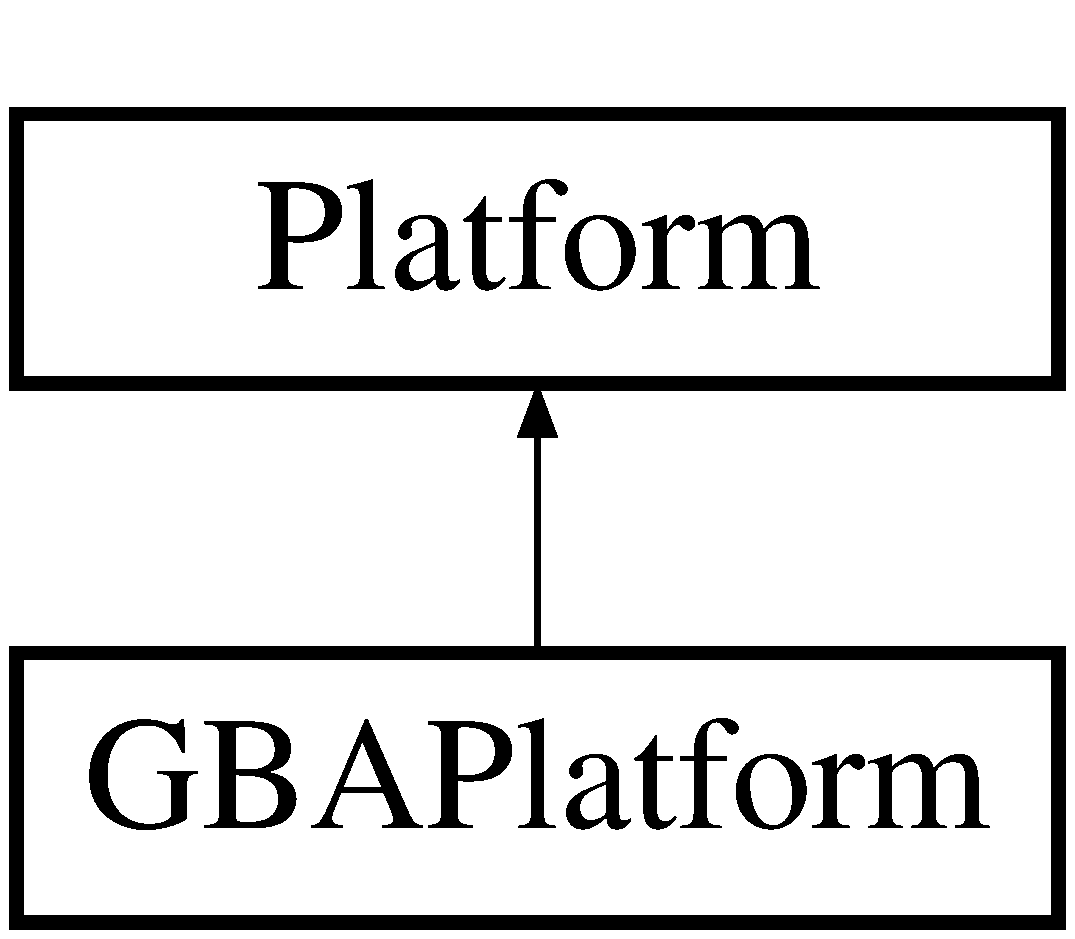
\includegraphics[height=2.000000cm]{class_g_b_a_platform}
\end{center}
\end{figure}


The documentation for this class was generated from the following files\-:\begin{DoxyCompactItemize}
\item 
G\-B\-A/include/platform/gba/platform.\-h\item 
G\-B\-A/src/platform/gba/platform.\-cpp\end{DoxyCompactItemize}

\hypertarget{class_g_b_a_sprite}{\section{G\-B\-A\-Sprite Class Reference}
\label{class_g_b_a_sprite}\index{G\-B\-A\-Sprite@{G\-B\-A\-Sprite}}
}
\subsection*{Public Attributes}
\begin{DoxyCompactItemize}
\item 
\hypertarget{class_g_b_a_sprite_a7ec5124ff20f8f8adbd90665bd63fd14}{int {\bfseries sprite\-Index}}\label{class_g_b_a_sprite_a7ec5124ff20f8f8adbd90665bd63fd14}

\end{DoxyCompactItemize}


The documentation for this class was generated from the following file\-:\begin{DoxyCompactItemize}
\item 
G\-B\-A/include/platform/gba/sprite.\-h\end{DoxyCompactItemize}

\hypertarget{class_g_b_a_tilemap}{\section{G\-B\-A\-Tilemap Class Reference}
\label{class_g_b_a_tilemap}\index{G\-B\-A\-Tilemap@{G\-B\-A\-Tilemap}}
}


Represents an entire background register for the display with simple functions for easy access to contained information.  




{\ttfamily \#include $<$tilemap.\-h$>$}

\subsection*{Public Member Functions}
\begin{DoxyCompactItemize}
\item 
\hyperlink{class_g_b_a_tilemap_af97e2847378557845a9677a22f54b3c8}{G\-B\-A\-Tilemap} (int bg\-Number, int x\-Off=0, int y\-Off=0)
\begin{DoxyCompactList}\small\item\em Initialises this B\-G, using standard charblock and screenblock numbering. \end{DoxyCompactList}\item 
\hyperlink{class_g_b_a_tilemap_a478fb5b5fe0274b6eba638b2643dd7a7}{G\-B\-A\-Tilemap} (int bg\-Number, int x\-Off, int y\-Off, int charblock, int screenblock)
\begin{DoxyCompactList}\small\item\em Initialises this B\-G, with specified charblock and screenblock numbering. \end{DoxyCompactList}\item 
void \hyperlink{class_g_b_a_tilemap_aa965c5ff1b0738466d2336ee02a329f4}{set\-Offset} (int x\-Off, int y\-Off)
\begin{DoxyCompactList}\small\item\em Sets the offset of this B\-G in absolute terms. \end{DoxyCompactList}\item 
void \hyperlink{class_g_b_a_tilemap_a153737902839590c84c81fc84415a39b}{offset} (int dx, int dy)
\begin{DoxyCompactList}\small\item\em Offsets this B\-G, relative to where it is. \end{DoxyCompactList}\item 
int \hyperlink{class_g_b_a_tilemap_a682ab6f960941dfde2bfc9c2f0e05796}{X} ()
\begin{DoxyCompactList}\small\item\em Getter for the current x value. \end{DoxyCompactList}\item 
int \hyperlink{class_g_b_a_tilemap_a6107b365da9ce64dec7eba818e889046}{Y} ()
\begin{DoxyCompactList}\small\item\em Getter for the current y value. \end{DoxyCompactList}\end{DoxyCompactItemize}
\subsection*{Private Member Functions}
\begin{DoxyCompactItemize}
\item 
void \hyperlink{class_g_b_a_tilemap_afc7eca23b7e262ac23465e68c9a9d23d}{init} (int bg\-Number, int x\-Off, int y\-Off, int charblock, int screenblock)
\begin{DoxyCompactList}\small\item\em Initialises the registers Params are all from constructor, check there for definition. \end{DoxyCompactList}\item 
void \hyperlink{class_g_b_a_tilemap_a0af625c6abcfb8e709f9719812ad0f46}{update\-Offset} ()
\begin{DoxyCompactList}\small\item\em Updates the offset registers to the current x and y values To be called straight after any changes to x or y are made. \end{DoxyCompactList}\end{DoxyCompactItemize}
\subsection*{Private Attributes}
\begin{DoxyCompactItemize}
\item 
volatile unsigned short $\ast$ \hyperlink{class_g_b_a_tilemap_a6582976ee722879c1f1c8424fedfa6dc}{control}
\begin{DoxyCompactList}\small\item\em Pointer to the control Register that specifies the charblock used etc. \end{DoxyCompactList}\item 
volatile unsigned short $\ast$ \hyperlink{class_g_b_a_tilemap_a4e59c0ad01395ffaa5b3e6ce978c41cf}{h\-Offset}
\begin{DoxyCompactList}\small\item\em Pointer to the Horizontal Offset register for this background. \end{DoxyCompactList}\item 
volatile unsigned short $\ast$ \hyperlink{class_g_b_a_tilemap_a1adc8cd141d27745c504a0f04ad107a1}{v\-Offset}
\begin{DoxyCompactList}\small\item\em Pointer to the Vertical Offset register for this background. \end{DoxyCompactList}\item 
int \hyperlink{class_g_b_a_tilemap_ae83d6511d021d12d55c9fa4613113998}{x}
\item 
int \hyperlink{class_g_b_a_tilemap_aa18154630ab0e96309fab9e7226a02a0}{y}
\begin{DoxyCompactList}\small\item\em Current x and y offsets. \end{DoxyCompactList}\end{DoxyCompactItemize}


\subsection{Detailed Description}
Represents an entire background register for the display with simple functions for easy access to contained information. 

\subsection{Constructor \& Destructor Documentation}
\hypertarget{class_g_b_a_tilemap_af97e2847378557845a9677a22f54b3c8}{\index{G\-B\-A\-Tilemap@{G\-B\-A\-Tilemap}!G\-B\-A\-Tilemap@{G\-B\-A\-Tilemap}}
\index{G\-B\-A\-Tilemap@{G\-B\-A\-Tilemap}!GBATilemap@{G\-B\-A\-Tilemap}}
\subsubsection[{G\-B\-A\-Tilemap}]{\setlength{\rightskip}{0pt plus 5cm}{\bf G\-B\-A\-Tilemap\-::\-G\-B\-A\-Tilemap} (
\begin{DoxyParamCaption}
\item[{int}]{bg\-Number, }
\item[{int}]{x\-Off = {\ttfamily 0}, }
\item[{int}]{y\-Off = {\ttfamily 0}}
\end{DoxyParamCaption}
)\hspace{0.3cm}{\ttfamily  \mbox{[}inline\mbox{]}}}}\label{class_g_b_a_tilemap_af97e2847378557845a9677a22f54b3c8}


Initialises this B\-G, using standard charblock and screenblock numbering. 


\begin{DoxyParams}{Parameters}
{\em bg\-Number} & A number between 0 and 3, for which background layer this is \\
\hline
{\em x\-Off} & The starting horizontal offset to the left \\
\hline
{\em y\-Off} & The starting vertical offset, downwards \\
\hline
\end{DoxyParams}
\begin{DoxyWarning}{Warning}
bg\-Numbers out of the 0-\/$>$3 range are placed at the ends of this range to avoid running off memory 
\end{DoxyWarning}
\hypertarget{class_g_b_a_tilemap_a478fb5b5fe0274b6eba638b2643dd7a7}{\index{G\-B\-A\-Tilemap@{G\-B\-A\-Tilemap}!G\-B\-A\-Tilemap@{G\-B\-A\-Tilemap}}
\index{G\-B\-A\-Tilemap@{G\-B\-A\-Tilemap}!GBATilemap@{G\-B\-A\-Tilemap}}
\subsubsection[{G\-B\-A\-Tilemap}]{\setlength{\rightskip}{0pt plus 5cm}{\bf G\-B\-A\-Tilemap\-::\-G\-B\-A\-Tilemap} (
\begin{DoxyParamCaption}
\item[{int}]{bg\-Number, }
\item[{int}]{x\-Off, }
\item[{int}]{y\-Off, }
\item[{int}]{charblock, }
\item[{int}]{screenblock}
\end{DoxyParamCaption}
)\hspace{0.3cm}{\ttfamily  \mbox{[}inline\mbox{]}}}}\label{class_g_b_a_tilemap_a478fb5b5fe0274b6eba638b2643dd7a7}


Initialises this B\-G, with specified charblock and screenblock numbering. 


\begin{DoxyParams}{Parameters}
{\em bg\-Number} & A number between 0 and 3, for which background layer this is \\
\hline
{\em x\-Off} & The starting horizontal offset to the left \\
\hline
{\em y\-Off} & The starting vertical offset, downwards \\
\hline
{\em charblock} & the charblock to be used for this background \\
\hline
{\em screenblock} & the screenblock to be used for this background \\
\hline
\end{DoxyParams}
\begin{DoxyWarning}{Warning}
bg\-Numbers and charblocks are forced into the range 0-\/$>$3, use charblock 0 first and ascend. 

screenblocks are forced into the range 30-\/$>$0; use screenblock 30 first and then descend. 
\end{DoxyWarning}


\subsection{Member Function Documentation}
\hypertarget{class_g_b_a_tilemap_afc7eca23b7e262ac23465e68c9a9d23d}{\index{G\-B\-A\-Tilemap@{G\-B\-A\-Tilemap}!init@{init}}
\index{init@{init}!GBATilemap@{G\-B\-A\-Tilemap}}
\subsubsection[{init}]{\setlength{\rightskip}{0pt plus 5cm}void {\bf G\-B\-A\-Tilemap\-::init} (
\begin{DoxyParamCaption}
\item[{int}]{bg\-Number, }
\item[{int}]{x\-Off, }
\item[{int}]{y\-Off, }
\item[{int}]{charblock, }
\item[{int}]{screenblock}
\end{DoxyParamCaption}
)\hspace{0.3cm}{\ttfamily  \mbox{[}inline, private\mbox{]}}}}\label{class_g_b_a_tilemap_afc7eca23b7e262ac23465e68c9a9d23d}


Initialises the registers Params are all from constructor, check there for definition. 

\hypertarget{class_g_b_a_tilemap_a153737902839590c84c81fc84415a39b}{\index{G\-B\-A\-Tilemap@{G\-B\-A\-Tilemap}!offset@{offset}}
\index{offset@{offset}!GBATilemap@{G\-B\-A\-Tilemap}}
\subsubsection[{offset}]{\setlength{\rightskip}{0pt plus 5cm}void {\bf G\-B\-A\-Tilemap\-::offset} (
\begin{DoxyParamCaption}
\item[{int}]{dx, }
\item[{int}]{dy}
\end{DoxyParamCaption}
)\hspace{0.3cm}{\ttfamily  \mbox{[}inline\mbox{]}}}}\label{class_g_b_a_tilemap_a153737902839590c84c81fc84415a39b}


Offsets this B\-G, relative to where it is. 


\begin{DoxyParams}{Parameters}
{\em dx} & the offset to be added to the left \\
\hline
{\em dy} & the offset to be added downwards \\
\hline
\end{DoxyParams}
\hypertarget{class_g_b_a_tilemap_aa965c5ff1b0738466d2336ee02a329f4}{\index{G\-B\-A\-Tilemap@{G\-B\-A\-Tilemap}!set\-Offset@{set\-Offset}}
\index{set\-Offset@{set\-Offset}!GBATilemap@{G\-B\-A\-Tilemap}}
\subsubsection[{set\-Offset}]{\setlength{\rightskip}{0pt plus 5cm}void {\bf G\-B\-A\-Tilemap\-::set\-Offset} (
\begin{DoxyParamCaption}
\item[{int}]{x\-Off, }
\item[{int}]{y\-Off}
\end{DoxyParamCaption}
)\hspace{0.3cm}{\ttfamily  \mbox{[}inline\mbox{]}}}}\label{class_g_b_a_tilemap_aa965c5ff1b0738466d2336ee02a329f4}


Sets the offset of this B\-G in absolute terms. 


\begin{DoxyParams}{Parameters}
{\em x\-Off} & the x offset of this B\-G, to the left \\
\hline
{\em y\-Off} & the y offset of this B\-G, downwards \\
\hline
\end{DoxyParams}
\hypertarget{class_g_b_a_tilemap_a0af625c6abcfb8e709f9719812ad0f46}{\index{G\-B\-A\-Tilemap@{G\-B\-A\-Tilemap}!update\-Offset@{update\-Offset}}
\index{update\-Offset@{update\-Offset}!GBATilemap@{G\-B\-A\-Tilemap}}
\subsubsection[{update\-Offset}]{\setlength{\rightskip}{0pt plus 5cm}void {\bf G\-B\-A\-Tilemap\-::update\-Offset} (
\begin{DoxyParamCaption}
{}
\end{DoxyParamCaption}
)\hspace{0.3cm}{\ttfamily  \mbox{[}inline, private\mbox{]}}}}\label{class_g_b_a_tilemap_a0af625c6abcfb8e709f9719812ad0f46}


Updates the offset registers to the current x and y values To be called straight after any changes to x or y are made. 

\hypertarget{class_g_b_a_tilemap_a682ab6f960941dfde2bfc9c2f0e05796}{\index{G\-B\-A\-Tilemap@{G\-B\-A\-Tilemap}!X@{X}}
\index{X@{X}!GBATilemap@{G\-B\-A\-Tilemap}}
\subsubsection[{X}]{\setlength{\rightskip}{0pt plus 5cm}int {\bf G\-B\-A\-Tilemap\-::\-X} (
\begin{DoxyParamCaption}
{}
\end{DoxyParamCaption}
)\hspace{0.3cm}{\ttfamily  \mbox{[}inline\mbox{]}}}}\label{class_g_b_a_tilemap_a682ab6f960941dfde2bfc9c2f0e05796}


Getter for the current x value. 

\hypertarget{class_g_b_a_tilemap_a6107b365da9ce64dec7eba818e889046}{\index{G\-B\-A\-Tilemap@{G\-B\-A\-Tilemap}!Y@{Y}}
\index{Y@{Y}!GBATilemap@{G\-B\-A\-Tilemap}}
\subsubsection[{Y}]{\setlength{\rightskip}{0pt plus 5cm}int {\bf G\-B\-A\-Tilemap\-::\-Y} (
\begin{DoxyParamCaption}
{}
\end{DoxyParamCaption}
)\hspace{0.3cm}{\ttfamily  \mbox{[}inline\mbox{]}}}}\label{class_g_b_a_tilemap_a6107b365da9ce64dec7eba818e889046}


Getter for the current y value. 



\subsection{Member Data Documentation}
\hypertarget{class_g_b_a_tilemap_a6582976ee722879c1f1c8424fedfa6dc}{\index{G\-B\-A\-Tilemap@{G\-B\-A\-Tilemap}!control@{control}}
\index{control@{control}!GBATilemap@{G\-B\-A\-Tilemap}}
\subsubsection[{control}]{\setlength{\rightskip}{0pt plus 5cm}volatile unsigned short$\ast$ {\bf G\-B\-A\-Tilemap\-::control}\hspace{0.3cm}{\ttfamily  \mbox{[}private\mbox{]}}}}\label{class_g_b_a_tilemap_a6582976ee722879c1f1c8424fedfa6dc}


Pointer to the control Register that specifies the charblock used etc. 

\hypertarget{class_g_b_a_tilemap_a4e59c0ad01395ffaa5b3e6ce978c41cf}{\index{G\-B\-A\-Tilemap@{G\-B\-A\-Tilemap}!h\-Offset@{h\-Offset}}
\index{h\-Offset@{h\-Offset}!GBATilemap@{G\-B\-A\-Tilemap}}
\subsubsection[{h\-Offset}]{\setlength{\rightskip}{0pt plus 5cm}volatile unsigned short$\ast$ {\bf G\-B\-A\-Tilemap\-::h\-Offset}\hspace{0.3cm}{\ttfamily  \mbox{[}private\mbox{]}}}}\label{class_g_b_a_tilemap_a4e59c0ad01395ffaa5b3e6ce978c41cf}


Pointer to the Horizontal Offset register for this background. 

\hypertarget{class_g_b_a_tilemap_a1adc8cd141d27745c504a0f04ad107a1}{\index{G\-B\-A\-Tilemap@{G\-B\-A\-Tilemap}!v\-Offset@{v\-Offset}}
\index{v\-Offset@{v\-Offset}!GBATilemap@{G\-B\-A\-Tilemap}}
\subsubsection[{v\-Offset}]{\setlength{\rightskip}{0pt plus 5cm}volatile unsigned short$\ast$ {\bf G\-B\-A\-Tilemap\-::v\-Offset}\hspace{0.3cm}{\ttfamily  \mbox{[}private\mbox{]}}}}\label{class_g_b_a_tilemap_a1adc8cd141d27745c504a0f04ad107a1}


Pointer to the Vertical Offset register for this background. 

\hypertarget{class_g_b_a_tilemap_ae83d6511d021d12d55c9fa4613113998}{\index{G\-B\-A\-Tilemap@{G\-B\-A\-Tilemap}!x@{x}}
\index{x@{x}!GBATilemap@{G\-B\-A\-Tilemap}}
\subsubsection[{x}]{\setlength{\rightskip}{0pt plus 5cm}int {\bf G\-B\-A\-Tilemap\-::x}\hspace{0.3cm}{\ttfamily  \mbox{[}private\mbox{]}}}}\label{class_g_b_a_tilemap_ae83d6511d021d12d55c9fa4613113998}
\hypertarget{class_g_b_a_tilemap_aa18154630ab0e96309fab9e7226a02a0}{\index{G\-B\-A\-Tilemap@{G\-B\-A\-Tilemap}!y@{y}}
\index{y@{y}!GBATilemap@{G\-B\-A\-Tilemap}}
\subsubsection[{y}]{\setlength{\rightskip}{0pt plus 5cm}int {\bf G\-B\-A\-Tilemap\-::y}\hspace{0.3cm}{\ttfamily  \mbox{[}private\mbox{]}}}}\label{class_g_b_a_tilemap_aa18154630ab0e96309fab9e7226a02a0}


Current x and y offsets. 



The documentation for this class was generated from the following file\-:\begin{DoxyCompactItemize}
\item 
G\-B\-A/include/platform/gba/\hyperlink{_g_b_a_2include_2platform_2gba_2tilemap_8h}{tilemap.\-h}\end{DoxyCompactItemize}

\hypertarget{struct_obj_affine}{\section{Obj\-Affine Struct Reference}
\label{struct_obj_affine}\index{Obj\-Affine@{Obj\-Affine}}
}


{\ttfamily \#include $<$gba.\-h$>$}

\subsection*{Public Attributes}
\begin{DoxyCompactItemize}
\item 
uint16\-\_\-t \hyperlink{struct_obj_affine_a5fdab3616d01dfd6d8440bc61f02a0e4}{pad0} \mbox{[}3\mbox{]}
\item 
int16\-\_\-t \hyperlink{struct_obj_affine_ae972edc100334aa968f79bb844763564}{pa}
\item 
uint16\-\_\-t \hyperlink{struct_obj_affine_a88ec2e52a1bdabd87a59c8246e30a2ec}{pad1} \mbox{[}3\mbox{]}
\item 
int16\-\_\-t \hyperlink{struct_obj_affine_a1f9024df291f5a7c32ce2444c8446144}{pb}
\item 
uint16\-\_\-t \hyperlink{struct_obj_affine_af6e35040fbfc316b1fa138e11752fa46}{pad2} \mbox{[}3\mbox{]}
\item 
int16\-\_\-t \hyperlink{struct_obj_affine_a2fd9f343a9c4a1dd3911f94db706e7ff}{pc}
\item 
uint16\-\_\-t \hyperlink{struct_obj_affine_af0a9dcf2ed70d86454ed49f44a894021}{pad3} \mbox{[}3\mbox{]}
\item 
int16\-\_\-t \hyperlink{struct_obj_affine_a1ae4cd5cf780b89479e4fe39d2377798}{pd}
\end{DoxyCompactItemize}


\subsection{Member Data Documentation}
\hypertarget{struct_obj_affine_ae972edc100334aa968f79bb844763564}{\index{Obj\-Affine@{Obj\-Affine}!pa@{pa}}
\index{pa@{pa}!ObjAffine@{Obj\-Affine}}
\subsubsection[{pa}]{\setlength{\rightskip}{0pt plus 5cm}int16\-\_\-t {\bf Obj\-Affine\-::pa}}}\label{struct_obj_affine_ae972edc100334aa968f79bb844763564}
\hypertarget{struct_obj_affine_a5fdab3616d01dfd6d8440bc61f02a0e4}{\index{Obj\-Affine@{Obj\-Affine}!pad0@{pad0}}
\index{pad0@{pad0}!ObjAffine@{Obj\-Affine}}
\subsubsection[{pad0}]{\setlength{\rightskip}{0pt plus 5cm}uint16\-\_\-t {\bf Obj\-Affine\-::pad0}\mbox{[}3\mbox{]}}}\label{struct_obj_affine_a5fdab3616d01dfd6d8440bc61f02a0e4}
\hypertarget{struct_obj_affine_a88ec2e52a1bdabd87a59c8246e30a2ec}{\index{Obj\-Affine@{Obj\-Affine}!pad1@{pad1}}
\index{pad1@{pad1}!ObjAffine@{Obj\-Affine}}
\subsubsection[{pad1}]{\setlength{\rightskip}{0pt plus 5cm}uint16\-\_\-t {\bf Obj\-Affine\-::pad1}\mbox{[}3\mbox{]}}}\label{struct_obj_affine_a88ec2e52a1bdabd87a59c8246e30a2ec}
\hypertarget{struct_obj_affine_af6e35040fbfc316b1fa138e11752fa46}{\index{Obj\-Affine@{Obj\-Affine}!pad2@{pad2}}
\index{pad2@{pad2}!ObjAffine@{Obj\-Affine}}
\subsubsection[{pad2}]{\setlength{\rightskip}{0pt plus 5cm}uint16\-\_\-t {\bf Obj\-Affine\-::pad2}\mbox{[}3\mbox{]}}}\label{struct_obj_affine_af6e35040fbfc316b1fa138e11752fa46}
\hypertarget{struct_obj_affine_af0a9dcf2ed70d86454ed49f44a894021}{\index{Obj\-Affine@{Obj\-Affine}!pad3@{pad3}}
\index{pad3@{pad3}!ObjAffine@{Obj\-Affine}}
\subsubsection[{pad3}]{\setlength{\rightskip}{0pt plus 5cm}uint16\-\_\-t {\bf Obj\-Affine\-::pad3}\mbox{[}3\mbox{]}}}\label{struct_obj_affine_af0a9dcf2ed70d86454ed49f44a894021}
\hypertarget{struct_obj_affine_a1f9024df291f5a7c32ce2444c8446144}{\index{Obj\-Affine@{Obj\-Affine}!pb@{pb}}
\index{pb@{pb}!ObjAffine@{Obj\-Affine}}
\subsubsection[{pb}]{\setlength{\rightskip}{0pt plus 5cm}int16\-\_\-t {\bf Obj\-Affine\-::pb}}}\label{struct_obj_affine_a1f9024df291f5a7c32ce2444c8446144}
\hypertarget{struct_obj_affine_a2fd9f343a9c4a1dd3911f94db706e7ff}{\index{Obj\-Affine@{Obj\-Affine}!pc@{pc}}
\index{pc@{pc}!ObjAffine@{Obj\-Affine}}
\subsubsection[{pc}]{\setlength{\rightskip}{0pt plus 5cm}int16\-\_\-t {\bf Obj\-Affine\-::pc}}}\label{struct_obj_affine_a2fd9f343a9c4a1dd3911f94db706e7ff}
\hypertarget{struct_obj_affine_a1ae4cd5cf780b89479e4fe39d2377798}{\index{Obj\-Affine@{Obj\-Affine}!pd@{pd}}
\index{pd@{pd}!ObjAffine@{Obj\-Affine}}
\subsubsection[{pd}]{\setlength{\rightskip}{0pt plus 5cm}int16\-\_\-t {\bf Obj\-Affine\-::pd}}}\label{struct_obj_affine_a1ae4cd5cf780b89479e4fe39d2377798}


The documentation for this struct was generated from the following file\-:\begin{DoxyCompactItemize}
\item 
G\-B\-A/lib/\hyperlink{gba_8h}{gba.\-h}\end{DoxyCompactItemize}

\hypertarget{struct_obj_attr}{\section{Obj\-Attr Struct Reference}
\label{struct_obj_attr}\index{Obj\-Attr@{Obj\-Attr}}
}


{\ttfamily \#include $<$gba.\-h$>$}

\subsection*{Public Attributes}
\begin{DoxyCompactItemize}
\item 
uint16\-\_\-t \hyperlink{struct_obj_attr_ab358a507b0ad6429e717941068d64f76}{attr0}
\item 
uint16\-\_\-t \hyperlink{struct_obj_attr_a86d659f745500f46f239d21a24b6ff3c}{attr1}
\item 
uint16\-\_\-t \hyperlink{struct_obj_attr_a43d6d720a9f684dbb0c23318ea9ce2ea}{attr2}
\item 
uint16\-\_\-t \hyperlink{struct_obj_attr_a4ce5fb46cf75eea5d97d939afe090802}{pad}
\end{DoxyCompactItemize}


\subsection{Member Data Documentation}
\hypertarget{struct_obj_attr_ab358a507b0ad6429e717941068d64f76}{\index{Obj\-Attr@{Obj\-Attr}!attr0@{attr0}}
\index{attr0@{attr0}!ObjAttr@{Obj\-Attr}}
\subsubsection[{attr0}]{\setlength{\rightskip}{0pt plus 5cm}uint16\-\_\-t {\bf Obj\-Attr\-::attr0}}}\label{struct_obj_attr_ab358a507b0ad6429e717941068d64f76}
\hypertarget{struct_obj_attr_a86d659f745500f46f239d21a24b6ff3c}{\index{Obj\-Attr@{Obj\-Attr}!attr1@{attr1}}
\index{attr1@{attr1}!ObjAttr@{Obj\-Attr}}
\subsubsection[{attr1}]{\setlength{\rightskip}{0pt plus 5cm}uint16\-\_\-t {\bf Obj\-Attr\-::attr1}}}\label{struct_obj_attr_a86d659f745500f46f239d21a24b6ff3c}
\hypertarget{struct_obj_attr_a43d6d720a9f684dbb0c23318ea9ce2ea}{\index{Obj\-Attr@{Obj\-Attr}!attr2@{attr2}}
\index{attr2@{attr2}!ObjAttr@{Obj\-Attr}}
\subsubsection[{attr2}]{\setlength{\rightskip}{0pt plus 5cm}uint16\-\_\-t {\bf Obj\-Attr\-::attr2}}}\label{struct_obj_attr_a43d6d720a9f684dbb0c23318ea9ce2ea}
\hypertarget{struct_obj_attr_a4ce5fb46cf75eea5d97d939afe090802}{\index{Obj\-Attr@{Obj\-Attr}!pad@{pad}}
\index{pad@{pad}!ObjAttr@{Obj\-Attr}}
\subsubsection[{pad}]{\setlength{\rightskip}{0pt plus 5cm}uint16\-\_\-t {\bf Obj\-Attr\-::pad}}}\label{struct_obj_attr_a4ce5fb46cf75eea5d97d939afe090802}


The documentation for this struct was generated from the following file\-:\begin{DoxyCompactItemize}
\item 
G\-B\-A/lib/\hyperlink{gba_8h}{gba.\-h}\end{DoxyCompactItemize}

\hypertarget{class_platform}{\section{Platform Class Reference}
\label{class_platform}\index{Platform@{Platform}}
}
Inheritance diagram for Platform\-:\begin{figure}[H]
\begin{center}
\leavevmode
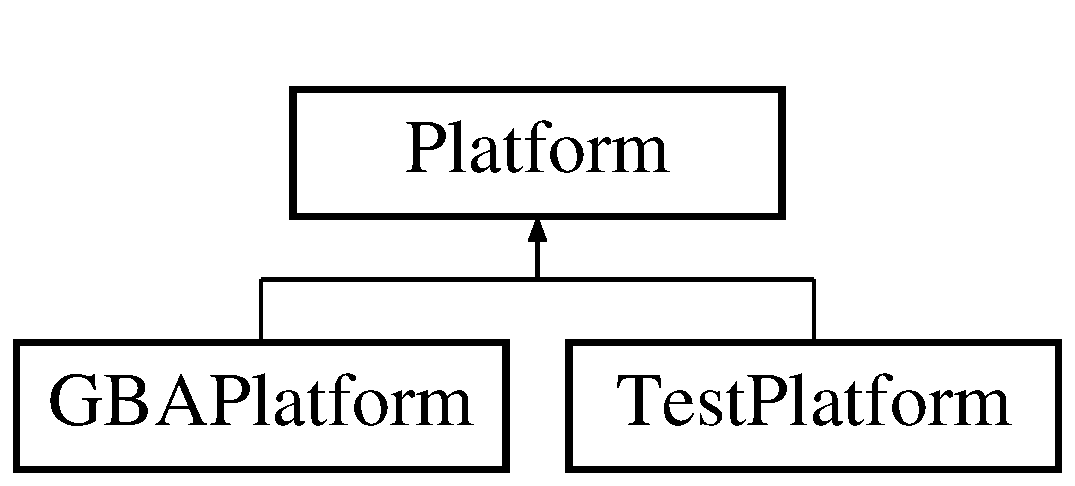
\includegraphics[height=2.000000cm]{class_platform}
\end{center}
\end{figure}
\subsection*{Public Member Functions}
\begin{DoxyCompactItemize}
\item 
\hypertarget{class_platform_ae1ce123f017fbf5949220a295320e11c}{void {\bfseries register\-Sprite} (\hyperlink{class_sprite}{Sprite} s)}\label{class_platform_ae1ce123f017fbf5949220a295320e11c}

\end{DoxyCompactItemize}


The documentation for this class was generated from the following file\-:\begin{DoxyCompactItemize}
\item 
Codebase/include/engine/platform.\-h\end{DoxyCompactItemize}

\hypertarget{class_player}{\section{Player Class Reference}
\label{class_player}\index{Player@{Player}}
}
\subsection*{Public Member Functions}
\begin{DoxyCompactItemize}
\item 
\hypertarget{class_player_a23d14d23255d0c0b291d750f6e9982b1}{{\bfseries Player} (int x\-Pos=0, int y\-Pos=0)}\label{class_player_a23d14d23255d0c0b291d750f6e9982b1}

\item 
\hypertarget{class_player_aa6a9d06e481e62626da52db9a6c79023}{void {\bfseries on\-Tick} ()}\label{class_player_aa6a9d06e481e62626da52db9a6c79023}

\item 
\hypertarget{class_player_abe2b38c7cda8362dcf1063eb1546d778}{void {\bfseries till\-Soil} ()}\label{class_player_abe2b38c7cda8362dcf1063eb1546d778}

\item 
\hypertarget{class_player_a552c0385003f06eae35485994b64b990}{void {\bfseries plant\-Seeds} ()}\label{class_player_a552c0385003f06eae35485994b64b990}

\item 
\hypertarget{class_player_a210c9c1c4ae5a84ceb467ed39d9117c3}{void {\bfseries water\-Soil} ()}\label{class_player_a210c9c1c4ae5a84ceb467ed39d9117c3}

\item 
\hypertarget{class_player_a5a013cb0ff7607a6968048780f25505b}{void {\bfseries harvest\-Crops} ()}\label{class_player_a5a013cb0ff7607a6968048780f25505b}

\item 
\hypertarget{class_player_a1cb7ff18fe3b07cc1dcd27519bde8329}{void {\bfseries update\-Position} ()}\label{class_player_a1cb7ff18fe3b07cc1dcd27519bde8329}

\item 
\hypertarget{class_player_a6818aa1ce188127d3e9d0209cdcbcdb4}{void {\bfseries get\-Inputs} ()}\label{class_player_a6818aa1ce188127d3e9d0209cdcbcdb4}

\end{DoxyCompactItemize}
\subsection*{Public Attributes}
\begin{DoxyCompactItemize}
\item 
\hypertarget{class_player_ad285b3cb25e4a46ca944b9a416c1b13f}{int {\bfseries x}}\label{class_player_ad285b3cb25e4a46ca944b9a416c1b13f}

\item 
\hypertarget{class_player_a6da29d6e3783c6028c92647bbde478f5}{int {\bfseries y}}\label{class_player_a6da29d6e3783c6028c92647bbde478f5}

\item 
\hypertarget{class_player_aac9bac60b3b27c77a1970f7e7999f5d5}{int {\bfseries sprite}}\label{class_player_aac9bac60b3b27c77a1970f7e7999f5d5}

\item 
\hypertarget{class_player_aa4536c3254fa3b774cd5b04483a3255b}{int {\bfseries anim\-Counter}}\label{class_player_aa4536c3254fa3b774cd5b04483a3255b}

\item 
\hypertarget{class_player_a6bcb0c797b73c3ea5e3d8ef797656c92}{int {\bfseries items} \mbox{[}10\mbox{]}}\label{class_player_a6bcb0c797b73c3ea5e3d8ef797656c92}

\item 
\hypertarget{class_player_aee04f54f61b45e5912b48fb9203cad38}{int {\bfseries tools} \mbox{[}10\mbox{]}}\label{class_player_aee04f54f61b45e5912b48fb9203cad38}

\item 
\hypertarget{class_player_aec48acba12d8b9245b4ba09146e0113c}{int {\bfseries current\-Tool}}\label{class_player_aec48acba12d8b9245b4ba09146e0113c}

\item 
\hypertarget{class_player_ab3f59417c9a2ee2d8a39a7a20f18dd51}{int {\bfseries current\-Item}}\label{class_player_ab3f59417c9a2ee2d8a39a7a20f18dd51}

\item 
\hypertarget{class_player_afb60fdad921bce05783ef2709e849c27}{Player\-State {\bfseries state}}\label{class_player_afb60fdad921bce05783ef2709e849c27}

\end{DoxyCompactItemize}
\subsection*{Static Public Attributes}
\begin{DoxyCompactItemize}
\item 
\hypertarget{class_player_af6cb41cc776191c988c8fa835fd12bc4}{static const int {\bfseries anim\-Counter\-Start} = 30}\label{class_player_af6cb41cc776191c988c8fa835fd12bc4}

\end{DoxyCompactItemize}


The documentation for this class was generated from the following files\-:\begin{DoxyCompactItemize}
\item 
Codebase/include/player.\-h\item 
Codebase/src/entity/player.\-cpp\end{DoxyCompactItemize}

\hypertarget{class_sprite}{\section{Sprite Class Reference}
\label{class_sprite}\index{Sprite@{Sprite}}
}


A 2\-D sprite graphic that can be moved, rotated and scaled Is non specific to any platform; making calls to the engine once a platform has been created.  




{\ttfamily \#include $<$sprite.\-h$>$}

\subsection*{Public Member Functions}
\begin{DoxyCompactItemize}
\item 
\hypertarget{class_sprite_a95a52b9a6911e359de3064fa6d3a5617}{{\bfseries Sprite} (int x\-Pos=0, int y\-Pos=0, int angle=0, float x\-Scale=1, float y\-Scale=1)}\label{class_sprite_a95a52b9a6911e359de3064fa6d3a5617}

\item 
\hypertarget{class_sprite_a94fe4c517497ba88a93b73cde72b29e8}{int {\bfseries x} ()}\label{class_sprite_a94fe4c517497ba88a93b73cde72b29e8}

\item 
\hypertarget{class_sprite_a2c5cebdd000b4c406432da3ce3a71cd6}{int {\bfseries y} ()}\label{class_sprite_a2c5cebdd000b4c406432da3ce3a71cd6}

\item 
\hypertarget{class_sprite_ad8d8da2bddcc3819ad6c1c43384b0349}{void {\bfseries x} (int x\-Position)}\label{class_sprite_ad8d8da2bddcc3819ad6c1c43384b0349}

\item 
\hypertarget{class_sprite_a3cc9eb64901a1b5a109a3fd1c7f548b5}{void {\bfseries y} (int y\-Position)}\label{class_sprite_a3cc9eb64901a1b5a109a3fd1c7f548b5}

\item 
\hypertarget{class_sprite_a2b89a3db5c84c3ae082cf71ec292f18b}{void {\bfseries move} (int dx, int dy)}\label{class_sprite_a2b89a3db5c84c3ae082cf71ec292f18b}

\item 
\hypertarget{class_sprite_a751b76bd42d5f922cee4f6890003b849}{void {\bfseries move\-To} (int x, int y)}\label{class_sprite_a751b76bd42d5f922cee4f6890003b849}

\item 
\hypertarget{class_sprite_a6e4553db94d974d88543b5a658f6c0c7}{int {\bfseries rotation} ()}\label{class_sprite_a6e4553db94d974d88543b5a658f6c0c7}

\item 
\hypertarget{class_sprite_a52ff92ae9e183b44153f1832b0fe8d9c}{void {\bfseries rotate} (int dw)}\label{class_sprite_a52ff92ae9e183b44153f1832b0fe8d9c}

\item 
\hypertarget{class_sprite_aceb65d178240d6abf04cd9c27ed0e095}{void {\bfseries rotation} (int angle)}\label{class_sprite_aceb65d178240d6abf04cd9c27ed0e095}

\item 
\hypertarget{class_sprite_a2163af37f17518f7c2a294f8ecc12b1d}{float {\bfseries scale\-X} ()}\label{class_sprite_a2163af37f17518f7c2a294f8ecc12b1d}

\item 
\hypertarget{class_sprite_a683509398c5d1098b0503eb223dd21f5}{float {\bfseries scale\-Y} ()}\label{class_sprite_a683509398c5d1098b0503eb223dd21f5}

\item 
\hypertarget{class_sprite_ae03819f524c4b85cc2b735a677ff6c25}{void {\bfseries scale\-X} (float)}\label{class_sprite_ae03819f524c4b85cc2b735a677ff6c25}

\item 
\hypertarget{class_sprite_a874153ccccd9304af8d7c19c51dedd74}{void {\bfseries scale\-Y} (float)}\label{class_sprite_a874153ccccd9304af8d7c19c51dedd74}

\item 
\hypertarget{class_sprite_a09ad4f5df5c625c44e31f02e625a40d0}{void {\bfseries scale} (float dx, float dy)}\label{class_sprite_a09ad4f5df5c625c44e31f02e625a40d0}

\item 
\hypertarget{class_sprite_a625a3ba4a2e647cf1a4d88afe9237bb3}{void {\bfseries scale\-To} (float x\-Scale, float y\-Scale)}\label{class_sprite_a625a3ba4a2e647cf1a4d88afe9237bb3}

\end{DoxyCompactItemize}


\subsection{Detailed Description}
A 2\-D sprite graphic that can be moved, rotated and scaled Is non specific to any platform; making calls to the engine once a platform has been created. 

The documentation for this class was generated from the following files\-:\begin{DoxyCompactItemize}
\item 
Codebase/include/engine/sprite.\-h\item 
Codebase/src/engine/graphics/sprite.\-cpp\end{DoxyCompactItemize}

\hypertarget{class_test_platform}{\section{Test\-Platform Class Reference}
\label{class_test_platform}\index{Test\-Platform@{Test\-Platform}}
}
Inheritance diagram for Test\-Platform\-:\begin{figure}[H]
\begin{center}
\leavevmode
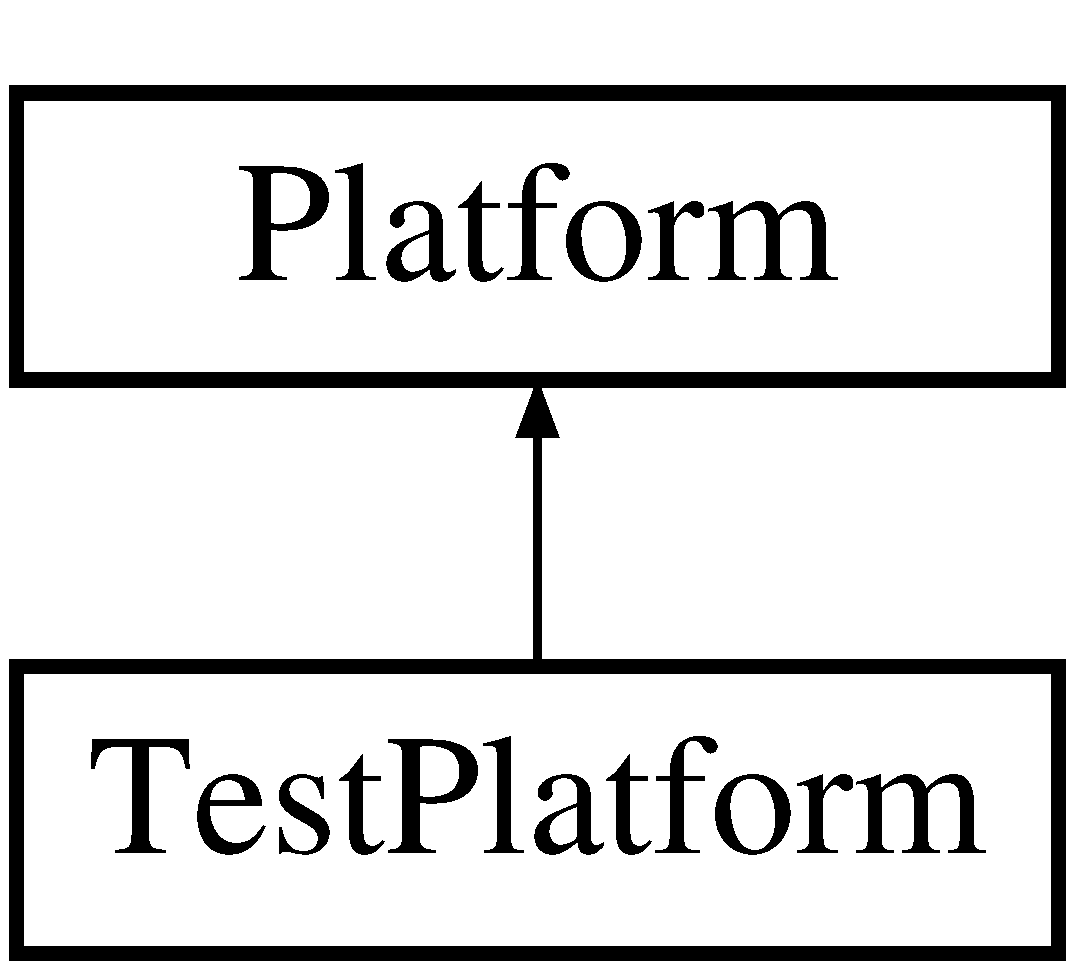
\includegraphics[height=2.000000cm]{class_test_platform}
\end{center}
\end{figure}
\subsection*{Public Member Functions}
\begin{DoxyCompactItemize}
\item 
\hypertarget{class_test_platform_ad20f3c7467d6bee028cfc55bf437fd11}{void {\bfseries register\-Sprite} (\hyperlink{class_sprite}{Sprite} s)}\label{class_test_platform_ad20f3c7467d6bee028cfc55bf437fd11}

\end{DoxyCompactItemize}


The documentation for this class was generated from the following file\-:\begin{DoxyCompactItemize}
\item 
Unit\-Tests/include/platform/test/platform.\-h\end{DoxyCompactItemize}

\hypertarget{class_tile}{\section{Tile Class Reference}
\label{class_tile}\index{Tile@{Tile}}
}


{\ttfamily \#include $<$tile.\-h$>$}



The documentation for this class was generated from the following file\-:\begin{DoxyCompactItemize}
\item 
Codebase/include/engine/\hyperlink{_codebase_2include_2engine_2tile_8h}{tile.\-h}\end{DoxyCompactItemize}

\hypertarget{class_tilemap}{\section{Tilemap Class Reference}
\label{class_tilemap}\index{Tilemap@{Tilemap}}
}


The documentation for this class was generated from the following file\-:\begin{DoxyCompactItemize}
\item 
Codebase/include/engine/tilemap.\-h\end{DoxyCompactItemize}

\chapter{File Documentation}
\hypertarget{animation_8h}{\section{Codebase/include/engine/animation.h File Reference}
\label{animation_8h}\index{Codebase/include/engine/animation.\-h@{Codebase/include/engine/animation.\-h}}
}

\hypertarget{bitmap_8h}{\section{Codebase/include/engine/bitmap.h File Reference}
\label{bitmap_8h}\index{Codebase/include/engine/bitmap.\-h@{Codebase/include/engine/bitmap.\-h}}
}
\subsection*{Classes}
\begin{DoxyCompactItemize}
\item 
class \hyperlink{class_bitmap}{Bitmap$<$ T $>$}
\begin{DoxyCompactList}\small\item\em \hyperlink{class_bitmap}{Bitmap} Resource, comprising of non-\/platform specific bitmap\-Data, and size data. On the G\-B\-A, the sizes are specifically limited to 8x8 amounts, as this is tile data. \end{DoxyCompactList}\end{DoxyCompactItemize}
\subsection*{Defines}
\begin{DoxyCompactItemize}
\item 
\#define \hyperlink{bitmap_8h_a4c7323b061431336257226a2c1e535e5}{E\-N\-A\-B\-L\-E\-I\-N\-T\-E\-L\-L\-I\-S\-E\-N\-S\-E}
\item 
\#define \hyperlink{bitmap_8h_a807ab484214b735ddabe3210ff935f3d}{L\-S\-\_\-\-B\-I\-T\-M\-A\-P}
\end{DoxyCompactItemize}


\subsection{Define Documentation}
\hypertarget{bitmap_8h_a4c7323b061431336257226a2c1e535e5}{\index{bitmap.\-h@{bitmap.\-h}!E\-N\-A\-B\-L\-E\-I\-N\-T\-E\-L\-L\-I\-S\-E\-N\-S\-E@{E\-N\-A\-B\-L\-E\-I\-N\-T\-E\-L\-L\-I\-S\-E\-N\-S\-E}}
\index{E\-N\-A\-B\-L\-E\-I\-N\-T\-E\-L\-L\-I\-S\-E\-N\-S\-E@{E\-N\-A\-B\-L\-E\-I\-N\-T\-E\-L\-L\-I\-S\-E\-N\-S\-E}!bitmap.h@{bitmap.\-h}}
\subsubsection[{E\-N\-A\-B\-L\-E\-I\-N\-T\-E\-L\-L\-I\-S\-E\-N\-S\-E}]{\setlength{\rightskip}{0pt plus 5cm}\#define {\bf E\-N\-A\-B\-L\-E\-I\-N\-T\-E\-L\-L\-I\-S\-E\-N\-S\-E}}}\label{bitmap_8h_a4c7323b061431336257226a2c1e535e5}
\hypertarget{bitmap_8h_a807ab484214b735ddabe3210ff935f3d}{\index{bitmap.\-h@{bitmap.\-h}!L\-S\-\_\-\-B\-I\-T\-M\-A\-P@{L\-S\-\_\-\-B\-I\-T\-M\-A\-P}}
\index{L\-S\-\_\-\-B\-I\-T\-M\-A\-P@{L\-S\-\_\-\-B\-I\-T\-M\-A\-P}!bitmap.h@{bitmap.\-h}}
\subsubsection[{L\-S\-\_\-\-B\-I\-T\-M\-A\-P}]{\setlength{\rightskip}{0pt plus 5cm}\#define {\bf L\-S\-\_\-\-B\-I\-T\-M\-A\-P}}}\label{bitmap_8h_a807ab484214b735ddabe3210ff935f3d}

\hypertarget{displaylist_8h}{\section{Codebase/include/engine/displaylist.h File Reference}
\label{displaylist_8h}\index{Codebase/include/engine/displaylist.\-h@{Codebase/include/engine/displaylist.\-h}}
}
{\ttfamily \#include \char`\"{}sprite.\-h\char`\"{}}\\*
{\ttfamily \#include $<$list$>$}\\*
\subsection*{Classes}
\begin{DoxyCompactItemize}
\item 
class \hyperlink{class_display_list}{Display\-List}
\end{DoxyCompactItemize}

\hypertarget{engine_8h}{\section{Codebase/include/engine/engine.h File Reference}
\label{engine_8h}\index{Codebase/include/engine/engine.\-h@{Codebase/include/engine/engine.\-h}}
}
{\ttfamily \#include \char`\"{}platform.\-h\char`\"{}}\\*
{\ttfamily \#include \char`\"{}displaylist.\-h\char`\"{}}\\*
{\ttfamily \#include \char`\"{}sprite.\-h\char`\"{}}\\*
{\ttfamily \#include \char`\"{}tile.\-h\char`\"{}}\\*
\subsection*{Functions}
\begin{DoxyCompactItemize}
\item 
void \hyperlink{engine_8h_a39d06d2ee579dcc720534747915d0590}{Set\-Tile} (int a, int b, int c, int d)
\item 
void \hyperlink{engine_8h_ac00b5b9b9b6ba79fcad74baec6adeab5}{set\-Platform} (\hyperlink{class_platform}{Platform} p)
\begin{DoxyCompactList}\small\item\em Sets the platform for development. \end{DoxyCompactList}\item 
void \hyperlink{engine_8h_a0195fe1e10473eb39f75c0d35e81000f}{new\-Sprite} (\hyperlink{class_sprite}{Sprite} s)
\begin{DoxyCompactList}\small\item\em Adds this sprite to the displaylist of sprites. \end{DoxyCompactList}\item 
void \hyperlink{engine_8h_af3f66c5984ad269df8f9412d24fde154}{new\-Tile} (\hyperlink{class_tile}{Tile} t)
\begin{DoxyCompactList}\small\item\em Adds a new tile into the game. \end{DoxyCompactList}\end{DoxyCompactItemize}
\subsection*{Variables}
\begin{DoxyCompactItemize}
\item 
\hyperlink{class_platform}{Platform} \hyperlink{engine_8h_a06826d0f95d583ccbc0a9a310ef202f5}{platform}
\item 
\hyperlink{class_display_list}{Display\-List} \hyperlink{engine_8h_a8cf8440bbe6bf3eb7aab8fb14f53c7ef}{display\-List}
\begin{DoxyCompactList}\small\item\em The display list that all drawn objects are sent to. \end{DoxyCompactList}\end{DoxyCompactItemize}


\subsection{Function Documentation}
\hypertarget{engine_8h_a0195fe1e10473eb39f75c0d35e81000f}{\index{engine.\-h@{engine.\-h}!new\-Sprite@{new\-Sprite}}
\index{new\-Sprite@{new\-Sprite}!engine.h@{engine.\-h}}
\subsubsection[{new\-Sprite}]{\setlength{\rightskip}{0pt plus 5cm}void {\bf new\-Sprite} (
\begin{DoxyParamCaption}
\item[{{\bf Sprite}}]{s}
\end{DoxyParamCaption}
)}}\label{engine_8h_a0195fe1e10473eb39f75c0d35e81000f}


Adds this sprite to the displaylist of sprites. 


\begin{DoxyParams}{Parameters}
{\em s} & The sprite to be added into the display list \\
\hline
\end{DoxyParams}
\hypertarget{engine_8h_af3f66c5984ad269df8f9412d24fde154}{\index{engine.\-h@{engine.\-h}!new\-Tile@{new\-Tile}}
\index{new\-Tile@{new\-Tile}!engine.h@{engine.\-h}}
\subsubsection[{new\-Tile}]{\setlength{\rightskip}{0pt plus 5cm}void {\bf new\-Tile} (
\begin{DoxyParamCaption}
\item[{{\bf Tile}}]{t}
\end{DoxyParamCaption}
)}}\label{engine_8h_af3f66c5984ad269df8f9412d24fde154}


Adds a new tile into the game. 


\begin{DoxyParams}{Parameters}
{\em t} & The tile to be added \\
\hline
\end{DoxyParams}
\hypertarget{engine_8h_ac00b5b9b9b6ba79fcad74baec6adeab5}{\index{engine.\-h@{engine.\-h}!set\-Platform@{set\-Platform}}
\index{set\-Platform@{set\-Platform}!engine.h@{engine.\-h}}
\subsubsection[{set\-Platform}]{\setlength{\rightskip}{0pt plus 5cm}void {\bf set\-Platform} (
\begin{DoxyParamCaption}
\item[{{\bf Platform}}]{p}
\end{DoxyParamCaption}
)}}\label{engine_8h_ac00b5b9b9b6ba79fcad74baec6adeab5}


Sets the platform for development. 


\begin{DoxyParams}{Parameters}
{\em p} & The platform to set up the engine for. \\
\hline
\end{DoxyParams}
\hypertarget{engine_8h_a39d06d2ee579dcc720534747915d0590}{\index{engine.\-h@{engine.\-h}!Set\-Tile@{Set\-Tile}}
\index{Set\-Tile@{Set\-Tile}!engine.h@{engine.\-h}}
\subsubsection[{Set\-Tile}]{\setlength{\rightskip}{0pt plus 5cm}void {\bf Set\-Tile} (
\begin{DoxyParamCaption}
\item[{int}]{a, }
\item[{int}]{b, }
\item[{int}]{c, }
\item[{int}]{d}
\end{DoxyParamCaption}
)}}\label{engine_8h_a39d06d2ee579dcc720534747915d0590}


\subsection{Variable Documentation}
\hypertarget{engine_8h_a8cf8440bbe6bf3eb7aab8fb14f53c7ef}{\index{engine.\-h@{engine.\-h}!display\-List@{display\-List}}
\index{display\-List@{display\-List}!engine.h@{engine.\-h}}
\subsubsection[{display\-List}]{\setlength{\rightskip}{0pt plus 5cm}{\bf Display\-List} {\bf display\-List}}}\label{engine_8h_a8cf8440bbe6bf3eb7aab8fb14f53c7ef}


The display list that all drawn objects are sent to. 

\hypertarget{engine_8h_a06826d0f95d583ccbc0a9a310ef202f5}{\index{engine.\-h@{engine.\-h}!platform@{platform}}
\index{platform@{platform}!engine.h@{engine.\-h}}
\subsubsection[{platform}]{\setlength{\rightskip}{0pt plus 5cm}{\bf Platform} {\bf platform}}}\label{engine_8h_a06826d0f95d583ccbc0a9a310ef202f5}
brief The platform being linked into the engine for development Takes calls from the engine and processes them for the specific platform hardware 
\hypertarget{game_8h}{\section{Codebase/include/engine/game.h File Reference}
\label{game_8h}\index{Codebase/include/engine/game.\-h@{Codebase/include/engine/game.\-h}}
}

\hypertarget{_codebase_2include_2engine_2platform_8h}{\section{Codebase/include/engine/platform.h File Reference}
\label{_codebase_2include_2engine_2platform_8h}\index{Codebase/include/engine/platform.\-h@{Codebase/include/engine/platform.\-h}}
}
{\ttfamily \#include \char`\"{}sprite.\-h\char`\"{}}\\*
\subsection*{Classes}
\begin{DoxyCompactItemize}
\item 
class \hyperlink{class_platform}{Platform}
\end{DoxyCompactItemize}

\hypertarget{_g_b_a_2include_2platform_2gba_2platform_8h}{\section{G\-B\-A/include/platform/gba/platform.h File Reference}
\label{_g_b_a_2include_2platform_2gba_2platform_8h}\index{G\-B\-A/include/platform/gba/platform.\-h@{G\-B\-A/include/platform/gba/platform.\-h}}
}
{\ttfamily \#include \char`\"{}engine$\backslash$platform.\-h\char`\"{}}\\*
\subsection*{Classes}
\begin{DoxyCompactItemize}
\item 
class \hyperlink{class_g_b_a_platform}{G\-B\-A\-Platform}
\end{DoxyCompactItemize}

\hypertarget{_unit_tests_2include_2platform_2test_2platform_8h}{\section{Unit\-Tests/include/platform/test/platform.h File Reference}
\label{_unit_tests_2include_2platform_2test_2platform_8h}\index{Unit\-Tests/include/platform/test/platform.\-h@{Unit\-Tests/include/platform/test/platform.\-h}}
}
{\ttfamily \#include \char`\"{}engine$\backslash$platform.\-h\char`\"{}}\\*
\subsection*{Classes}
\begin{DoxyCompactItemize}
\item 
class \hyperlink{class_test_platform}{Test\-Platform}
\end{DoxyCompactItemize}

\hypertarget{sound_8h}{\section{Codebase/include/engine/sound.h File Reference}
\label{sound_8h}\index{Codebase/include/engine/sound.\-h@{Codebase/include/engine/sound.\-h}}
}
{\ttfamily \#include \char`\"{}../../common/interface.\-h\char`\"{}}\\*

\hypertarget{_codebase_2include_2engine_2sprite_8h}{\section{Codebase/include/engine/sprite.h File Reference}
\label{_codebase_2include_2engine_2sprite_8h}\index{Codebase/include/engine/sprite.\-h@{Codebase/include/engine/sprite.\-h}}
}
{\ttfamily \#include \char`\"{}bitmap.\-h\char`\"{}}\\*
\subsection*{Classes}
\begin{DoxyCompactItemize}
\item 
class \hyperlink{class_sprite}{Sprite}
\begin{DoxyCompactList}\small\item\em A 2\-D sprite graphic that can be moved, rotated and scaled Is non specific to any platform; making calls to the engine once a platform has been created. \end{DoxyCompactList}\end{DoxyCompactItemize}

\hypertarget{_g_b_a_2include_2platform_2gba_2sprite_8h}{\section{G\-B\-A/include/platform/gba/sprite.h File Reference}
\label{_g_b_a_2include_2platform_2gba_2sprite_8h}\index{G\-B\-A/include/platform/gba/sprite.\-h@{G\-B\-A/include/platform/gba/sprite.\-h}}
}
\subsection*{Classes}
\begin{DoxyCompactItemize}
\item 
class \hyperlink{class_g_b_a_sprite}{G\-B\-A\-Sprite}
\end{DoxyCompactItemize}

\hypertarget{stage_8h}{\section{Codebase/include/engine/stage.h File Reference}
\label{stage_8h}\index{Codebase/include/engine/stage.\-h@{Codebase/include/engine/stage.\-h}}
}

\hypertarget{_codebase_2include_2engine_2tile_8h}{\section{Codebase/include/engine/tile.h File Reference}
\label{_codebase_2include_2engine_2tile_8h}\index{Codebase/include/engine/tile.\-h@{Codebase/include/engine/tile.\-h}}
}
\subsection*{Classes}
\begin{DoxyCompactItemize}
\item 
class \hyperlink{class_tile}{Tile}
\end{DoxyCompactItemize}

\hypertarget{_g_b_a_2include_2platform_2gba_2tile_8h}{\section{G\-B\-A/include/platform/gba/tile.h File Reference}
\label{_g_b_a_2include_2platform_2gba_2tile_8h}\index{G\-B\-A/include/platform/gba/tile.\-h@{G\-B\-A/include/platform/gba/tile.\-h}}
}

\hypertarget{_codebase_2include_2engine_2tilemap_8h}{\section{Codebase/include/engine/tilemap.h File Reference}
\label{_codebase_2include_2engine_2tilemap_8h}\index{Codebase/include/engine/tilemap.\-h@{Codebase/include/engine/tilemap.\-h}}
}
\subsection*{Classes}
\begin{DoxyCompactItemize}
\item 
class \hyperlink{class_tilemap}{Tilemap}
\end{DoxyCompactItemize}

\hypertarget{_g_b_a_2include_2platform_2gba_2tilemap_8h}{\section{G\-B\-A/include/platform/gba/tilemap.h File Reference}
\label{_g_b_a_2include_2platform_2gba_2tilemap_8h}\index{G\-B\-A/include/platform/gba/tilemap.\-h@{G\-B\-A/include/platform/gba/tilemap.\-h}}
}
{\ttfamily \#include \char`\"{}../../../lib/gba.\-h\char`\"{}}\\*
\subsection*{Classes}
\begin{DoxyCompactItemize}
\item 
class \hyperlink{class_g_b_a_tilemap}{G\-B\-A\-Tilemap}
\begin{DoxyCompactList}\small\item\em Represents an entire background register for the display with simple functions for easy access to contained information. \end{DoxyCompactList}\end{DoxyCompactItemize}
\subsection*{Defines}
\begin{DoxyCompactItemize}
\item 
\#define \hyperlink{_g_b_a_2include_2platform_2gba_2tilemap_8h_af63cf11dbe36a84249e757cf77e11ac8}{R\-E\-G\-\_\-\-B\-G\-C\-N\-T\-\_\-\-B\-A\-S\-E}~\hyperlink{gba_8h_a33c5a5c83c922b14274bf3da8ecbd3a8}{R\-E\-G\-I\-S\-T\-E\-R}(uint16\-\_\-t, 0x4000008)
\begin{DoxyCompactList}\small\item\em Holds functionality corresponding to the R\-E\-G\-\_\-\-B\-G-\/-\/-\/ Registers from A.\-Sampson's \hyperlink{gba_8h}{gba.\-h} file. It is designed to give easier access to the data in these, and allow for simple initialisation in a constructor There are no known issues of efficiency in using this compared to direct register access. \end{DoxyCompactList}\item 
\#define \hyperlink{_g_b_a_2include_2platform_2gba_2tilemap_8h_a06e0b351131fc01f619385a080c69533}{R\-E\-G\-\_\-\-B\-G\-H\-O\-F\-S\-\_\-\-B\-A\-S\-E}~\hyperlink{gba_8h_a33c5a5c83c922b14274bf3da8ecbd3a8}{R\-E\-G\-I\-S\-T\-E\-R}(uint16\-\_\-t, 0x400001\-C)
\item 
\#define \hyperlink{_g_b_a_2include_2platform_2gba_2tilemap_8h_a82224958bd244cc1baf329ee22b7eb28}{R\-E\-G\-\_\-\-B\-G\-V\-O\-F\-S\-\_\-\-B\-A\-S\-E}~\hyperlink{gba_8h_a33c5a5c83c922b14274bf3da8ecbd3a8}{R\-E\-G\-I\-S\-T\-E\-R}(uint16\-\_\-t, 0x4000012)
\end{DoxyCompactItemize}


\subsection{Define Documentation}
\hypertarget{_g_b_a_2include_2platform_2gba_2tilemap_8h_af63cf11dbe36a84249e757cf77e11ac8}{\index{G\-B\-A/include/platform/gba/tilemap.\-h@{G\-B\-A/include/platform/gba/tilemap.\-h}!R\-E\-G\-\_\-\-B\-G\-C\-N\-T\-\_\-\-B\-A\-S\-E@{R\-E\-G\-\_\-\-B\-G\-C\-N\-T\-\_\-\-B\-A\-S\-E}}
\index{R\-E\-G\-\_\-\-B\-G\-C\-N\-T\-\_\-\-B\-A\-S\-E@{R\-E\-G\-\_\-\-B\-G\-C\-N\-T\-\_\-\-B\-A\-S\-E}!GBA/include/platform/gba/tilemap.h@{G\-B\-A/include/platform/gba/tilemap.\-h}}
\subsubsection[{R\-E\-G\-\_\-\-B\-G\-C\-N\-T\-\_\-\-B\-A\-S\-E}]{\setlength{\rightskip}{0pt plus 5cm}\#define {\bf R\-E\-G\-\_\-\-B\-G\-C\-N\-T\-\_\-\-B\-A\-S\-E}~{\bf R\-E\-G\-I\-S\-T\-E\-R}(uint16\-\_\-t, 0x4000008)}}\label{_g_b_a_2include_2platform_2gba_2tilemap_8h_af63cf11dbe36a84249e757cf77e11ac8}


Holds functionality corresponding to the R\-E\-G\-\_\-\-B\-G-\/-\/-\/ Registers from A.\-Sampson's \hyperlink{gba_8h}{gba.\-h} file. It is designed to give easier access to the data in these, and allow for simple initialisation in a constructor There are no known issues of efficiency in using this compared to direct register access. 

\hypertarget{_g_b_a_2include_2platform_2gba_2tilemap_8h_a06e0b351131fc01f619385a080c69533}{\index{G\-B\-A/include/platform/gba/tilemap.\-h@{G\-B\-A/include/platform/gba/tilemap.\-h}!R\-E\-G\-\_\-\-B\-G\-H\-O\-F\-S\-\_\-\-B\-A\-S\-E@{R\-E\-G\-\_\-\-B\-G\-H\-O\-F\-S\-\_\-\-B\-A\-S\-E}}
\index{R\-E\-G\-\_\-\-B\-G\-H\-O\-F\-S\-\_\-\-B\-A\-S\-E@{R\-E\-G\-\_\-\-B\-G\-H\-O\-F\-S\-\_\-\-B\-A\-S\-E}!GBA/include/platform/gba/tilemap.h@{G\-B\-A/include/platform/gba/tilemap.\-h}}
\subsubsection[{R\-E\-G\-\_\-\-B\-G\-H\-O\-F\-S\-\_\-\-B\-A\-S\-E}]{\setlength{\rightskip}{0pt plus 5cm}\#define {\bf R\-E\-G\-\_\-\-B\-G\-H\-O\-F\-S\-\_\-\-B\-A\-S\-E}~{\bf R\-E\-G\-I\-S\-T\-E\-R}(uint16\-\_\-t, 0x400001\-C)}}\label{_g_b_a_2include_2platform_2gba_2tilemap_8h_a06e0b351131fc01f619385a080c69533}
\hypertarget{_g_b_a_2include_2platform_2gba_2tilemap_8h_a82224958bd244cc1baf329ee22b7eb28}{\index{G\-B\-A/include/platform/gba/tilemap.\-h@{G\-B\-A/include/platform/gba/tilemap.\-h}!R\-E\-G\-\_\-\-B\-G\-V\-O\-F\-S\-\_\-\-B\-A\-S\-E@{R\-E\-G\-\_\-\-B\-G\-V\-O\-F\-S\-\_\-\-B\-A\-S\-E}}
\index{R\-E\-G\-\_\-\-B\-G\-V\-O\-F\-S\-\_\-\-B\-A\-S\-E@{R\-E\-G\-\_\-\-B\-G\-V\-O\-F\-S\-\_\-\-B\-A\-S\-E}!GBA/include/platform/gba/tilemap.h@{G\-B\-A/include/platform/gba/tilemap.\-h}}
\subsubsection[{R\-E\-G\-\_\-\-B\-G\-V\-O\-F\-S\-\_\-\-B\-A\-S\-E}]{\setlength{\rightskip}{0pt plus 5cm}\#define {\bf R\-E\-G\-\_\-\-B\-G\-V\-O\-F\-S\-\_\-\-B\-A\-S\-E}~{\bf R\-E\-G\-I\-S\-T\-E\-R}(uint16\-\_\-t, 0x4000012)}}\label{_g_b_a_2include_2platform_2gba_2tilemap_8h_a82224958bd244cc1baf329ee22b7eb28}

\hypertarget{player_8h}{\section{Codebase/include/player.h File Reference}
\label{player_8h}\index{Codebase/include/player.\-h@{Codebase/include/player.\-h}}
}
\subsection*{Classes}
\begin{DoxyCompactItemize}
\item 
class \hyperlink{class_player}{Player}
\end{DoxyCompactItemize}

\hypertarget{world_8h}{\section{Codebase/include/world.h File Reference}
\label{world_8h}\index{Codebase/include/world.\-h@{Codebase/include/world.\-h}}
}
\subsection*{Classes}
\begin{DoxyCompactItemize}
\item 
struct \hyperlink{struct_block}{Block}
\end{DoxyCompactItemize}
\subsection*{Defines}
\begin{DoxyCompactItemize}
\item 
\#define \hyperlink{world_8h_a5a630da772729866ff66a55000286f85}{W\-A\-L\-K\-A\-B\-L\-E\-\_\-\-O\-F\-F\-S\-E\-T}~8
\item 
\#define \hyperlink{world_8h_ac1d55619b505d2d4049a38e3b45eb376}{P\-L\-A\-N\-T\-E\-D\-\_\-\-O\-F\-F\-S\-E\-T}~7
\item 
\#define \hyperlink{world_8h_aee2a3b3c8d5158ae566c371e2f15a3dc}{T\-I\-L\-L\-E\-D\-\_\-\-O\-F\-F\-S\-E\-T}~6
\item 
\#define \hyperlink{world_8h_a895f60dd04f6832bfcb0160f526d348e}{F\-A\-R\-M\-A\-B\-L\-E\-\_\-\-O\-F\-F\-S\-E\-T}~5
\item 
\#define \hyperlink{world_8h_aa037a6d6a4f04d51c7ec1c9ee9054e76}{M\-A\-P\-\_\-\-W\-I\-D\-T\-H}~30
\item 
\#define \hyperlink{world_8h_a529d5ebb449edf31d9835d13f4fb9f89}{M\-A\-P\-\_\-\-H\-E\-I\-G\-H\-T}~20
\end{DoxyCompactItemize}
\subsection*{Functions}
\begin{DoxyCompactItemize}
\item 
void \hyperlink{world_8h_ae54812e7472e05cfa904971d0628100d}{harvest} (int x, int y)
\item 
void \hyperlink{world_8h_a34fa603ed92a3b09f8c66035affdcfca}{water} (int x, int y)
\item 
void \hyperlink{world_8h_a092fbcfb81dc9a912bb14b2d7aba4386}{till} (int x, int y)
\item 
void \hyperlink{world_8h_a3ffd29964d7ed1ccc25d17acd5d7033f}{plant} (int x, int y)
\end{DoxyCompactItemize}
\subsection*{Variables}
\begin{DoxyCompactItemize}
\item 
\hyperlink{struct_block}{Block} \hyperlink{world_8h_a5dd02d40be82e3c9972b53ca39d6256a}{map} \mbox{[}\hyperlink{world_8h_a529d5ebb449edf31d9835d13f4fb9f89}{M\-A\-P\-\_\-\-H\-E\-I\-G\-H\-T}\mbox{]}\mbox{[}\hyperlink{world_8h_aa037a6d6a4f04d51c7ec1c9ee9054e76}{M\-A\-P\-\_\-\-W\-I\-D\-T\-H}\mbox{]}
\end{DoxyCompactItemize}


\subsection{Define Documentation}
\hypertarget{world_8h_a895f60dd04f6832bfcb0160f526d348e}{\index{world.\-h@{world.\-h}!F\-A\-R\-M\-A\-B\-L\-E\-\_\-\-O\-F\-F\-S\-E\-T@{F\-A\-R\-M\-A\-B\-L\-E\-\_\-\-O\-F\-F\-S\-E\-T}}
\index{F\-A\-R\-M\-A\-B\-L\-E\-\_\-\-O\-F\-F\-S\-E\-T@{F\-A\-R\-M\-A\-B\-L\-E\-\_\-\-O\-F\-F\-S\-E\-T}!world.h@{world.\-h}}
\subsubsection[{F\-A\-R\-M\-A\-B\-L\-E\-\_\-\-O\-F\-F\-S\-E\-T}]{\setlength{\rightskip}{0pt plus 5cm}\#define {\bf F\-A\-R\-M\-A\-B\-L\-E\-\_\-\-O\-F\-F\-S\-E\-T}~5}}\label{world_8h_a895f60dd04f6832bfcb0160f526d348e}
\hypertarget{world_8h_a529d5ebb449edf31d9835d13f4fb9f89}{\index{world.\-h@{world.\-h}!M\-A\-P\-\_\-\-H\-E\-I\-G\-H\-T@{M\-A\-P\-\_\-\-H\-E\-I\-G\-H\-T}}
\index{M\-A\-P\-\_\-\-H\-E\-I\-G\-H\-T@{M\-A\-P\-\_\-\-H\-E\-I\-G\-H\-T}!world.h@{world.\-h}}
\subsubsection[{M\-A\-P\-\_\-\-H\-E\-I\-G\-H\-T}]{\setlength{\rightskip}{0pt plus 5cm}\#define {\bf M\-A\-P\-\_\-\-H\-E\-I\-G\-H\-T}~20}}\label{world_8h_a529d5ebb449edf31d9835d13f4fb9f89}
\hypertarget{world_8h_aa037a6d6a4f04d51c7ec1c9ee9054e76}{\index{world.\-h@{world.\-h}!M\-A\-P\-\_\-\-W\-I\-D\-T\-H@{M\-A\-P\-\_\-\-W\-I\-D\-T\-H}}
\index{M\-A\-P\-\_\-\-W\-I\-D\-T\-H@{M\-A\-P\-\_\-\-W\-I\-D\-T\-H}!world.h@{world.\-h}}
\subsubsection[{M\-A\-P\-\_\-\-W\-I\-D\-T\-H}]{\setlength{\rightskip}{0pt plus 5cm}\#define {\bf M\-A\-P\-\_\-\-W\-I\-D\-T\-H}~30}}\label{world_8h_aa037a6d6a4f04d51c7ec1c9ee9054e76}
\hypertarget{world_8h_ac1d55619b505d2d4049a38e3b45eb376}{\index{world.\-h@{world.\-h}!P\-L\-A\-N\-T\-E\-D\-\_\-\-O\-F\-F\-S\-E\-T@{P\-L\-A\-N\-T\-E\-D\-\_\-\-O\-F\-F\-S\-E\-T}}
\index{P\-L\-A\-N\-T\-E\-D\-\_\-\-O\-F\-F\-S\-E\-T@{P\-L\-A\-N\-T\-E\-D\-\_\-\-O\-F\-F\-S\-E\-T}!world.h@{world.\-h}}
\subsubsection[{P\-L\-A\-N\-T\-E\-D\-\_\-\-O\-F\-F\-S\-E\-T}]{\setlength{\rightskip}{0pt plus 5cm}\#define {\bf P\-L\-A\-N\-T\-E\-D\-\_\-\-O\-F\-F\-S\-E\-T}~7}}\label{world_8h_ac1d55619b505d2d4049a38e3b45eb376}
\hypertarget{world_8h_aee2a3b3c8d5158ae566c371e2f15a3dc}{\index{world.\-h@{world.\-h}!T\-I\-L\-L\-E\-D\-\_\-\-O\-F\-F\-S\-E\-T@{T\-I\-L\-L\-E\-D\-\_\-\-O\-F\-F\-S\-E\-T}}
\index{T\-I\-L\-L\-E\-D\-\_\-\-O\-F\-F\-S\-E\-T@{T\-I\-L\-L\-E\-D\-\_\-\-O\-F\-F\-S\-E\-T}!world.h@{world.\-h}}
\subsubsection[{T\-I\-L\-L\-E\-D\-\_\-\-O\-F\-F\-S\-E\-T}]{\setlength{\rightskip}{0pt plus 5cm}\#define {\bf T\-I\-L\-L\-E\-D\-\_\-\-O\-F\-F\-S\-E\-T}~6}}\label{world_8h_aee2a3b3c8d5158ae566c371e2f15a3dc}
\hypertarget{world_8h_a5a630da772729866ff66a55000286f85}{\index{world.\-h@{world.\-h}!W\-A\-L\-K\-A\-B\-L\-E\-\_\-\-O\-F\-F\-S\-E\-T@{W\-A\-L\-K\-A\-B\-L\-E\-\_\-\-O\-F\-F\-S\-E\-T}}
\index{W\-A\-L\-K\-A\-B\-L\-E\-\_\-\-O\-F\-F\-S\-E\-T@{W\-A\-L\-K\-A\-B\-L\-E\-\_\-\-O\-F\-F\-S\-E\-T}!world.h@{world.\-h}}
\subsubsection[{W\-A\-L\-K\-A\-B\-L\-E\-\_\-\-O\-F\-F\-S\-E\-T}]{\setlength{\rightskip}{0pt plus 5cm}\#define {\bf W\-A\-L\-K\-A\-B\-L\-E\-\_\-\-O\-F\-F\-S\-E\-T}~8}}\label{world_8h_a5a630da772729866ff66a55000286f85}


\subsection{Function Documentation}
\hypertarget{world_8h_ae54812e7472e05cfa904971d0628100d}{\index{world.\-h@{world.\-h}!harvest@{harvest}}
\index{harvest@{harvest}!world.h@{world.\-h}}
\subsubsection[{harvest}]{\setlength{\rightskip}{0pt plus 5cm}void {\bf harvest} (
\begin{DoxyParamCaption}
\item[{int}]{x, }
\item[{int}]{y}
\end{DoxyParamCaption}
)}}\label{world_8h_ae54812e7472e05cfa904971d0628100d}
\hypertarget{world_8h_a3ffd29964d7ed1ccc25d17acd5d7033f}{\index{world.\-h@{world.\-h}!plant@{plant}}
\index{plant@{plant}!world.h@{world.\-h}}
\subsubsection[{plant}]{\setlength{\rightskip}{0pt plus 5cm}void {\bf plant} (
\begin{DoxyParamCaption}
\item[{int}]{x, }
\item[{int}]{y}
\end{DoxyParamCaption}
)}}\label{world_8h_a3ffd29964d7ed1ccc25d17acd5d7033f}
\hypertarget{world_8h_a092fbcfb81dc9a912bb14b2d7aba4386}{\index{world.\-h@{world.\-h}!till@{till}}
\index{till@{till}!world.h@{world.\-h}}
\subsubsection[{till}]{\setlength{\rightskip}{0pt plus 5cm}void {\bf till} (
\begin{DoxyParamCaption}
\item[{int}]{x, }
\item[{int}]{y}
\end{DoxyParamCaption}
)}}\label{world_8h_a092fbcfb81dc9a912bb14b2d7aba4386}
\hypertarget{world_8h_a34fa603ed92a3b09f8c66035affdcfca}{\index{world.\-h@{world.\-h}!water@{water}}
\index{water@{water}!world.h@{world.\-h}}
\subsubsection[{water}]{\setlength{\rightskip}{0pt plus 5cm}void {\bf water} (
\begin{DoxyParamCaption}
\item[{int}]{x, }
\item[{int}]{y}
\end{DoxyParamCaption}
)}}\label{world_8h_a34fa603ed92a3b09f8c66035affdcfca}


\subsection{Variable Documentation}
\hypertarget{world_8h_a5dd02d40be82e3c9972b53ca39d6256a}{\index{world.\-h@{world.\-h}!map@{map}}
\index{map@{map}!world.h@{world.\-h}}
\subsubsection[{map}]{\setlength{\rightskip}{0pt plus 5cm}{\bf Block} {\bf map}\mbox{[}{\bf M\-A\-P\-\_\-\-H\-E\-I\-G\-H\-T}\mbox{]}\mbox{[}{\bf M\-A\-P\-\_\-\-W\-I\-D\-T\-H}\mbox{]}}}\label{world_8h_a5dd02d40be82e3c9972b53ca39d6256a}

\hypertarget{engine_8cpp}{\section{Codebase/src/engine/engine.cpp File Reference}
\label{engine_8cpp}\index{Codebase/src/engine/engine.\-cpp@{Codebase/src/engine/engine.\-cpp}}
}
{\ttfamily \#include \char`\"{}engine$\backslash$engine.\-h\char`\"{}}\\*
{\ttfamily \#include \char`\"{}engine$\backslash$platform.\-h\char`\"{}}\\*
{\ttfamily \#include \char`\"{}engine$\backslash$sprite.\-h\char`\"{}}\\*
\subsection*{Functions}
\begin{DoxyCompactItemize}
\item 
void \hyperlink{engine_8cpp_ac00b5b9b9b6ba79fcad74baec6adeab5}{set\-Platform} (\hyperlink{class_platform}{Platform} p)
\item 
void \hyperlink{engine_8cpp_a37ac4a4be26e0c04fc76272f695aaad4}{register\-Sprite} (\hyperlink{class_sprite}{Sprite} s)
\end{DoxyCompactItemize}
\subsection*{Variables}
\begin{DoxyCompactItemize}
\item 
\hyperlink{class_platform}{Platform} \hyperlink{engine_8cpp_a06826d0f95d583ccbc0a9a310ef202f5}{platform}
\end{DoxyCompactItemize}


\subsection{Function Documentation}
\hypertarget{engine_8cpp_a37ac4a4be26e0c04fc76272f695aaad4}{\index{engine.\-cpp@{engine.\-cpp}!register\-Sprite@{register\-Sprite}}
\index{register\-Sprite@{register\-Sprite}!engine.cpp@{engine.\-cpp}}
\subsubsection[{register\-Sprite}]{\setlength{\rightskip}{0pt plus 5cm}void {\bf register\-Sprite} (
\begin{DoxyParamCaption}
\item[{{\bf Sprite}}]{s}
\end{DoxyParamCaption}
)}}\label{engine_8cpp_a37ac4a4be26e0c04fc76272f695aaad4}
\hypertarget{engine_8cpp_ac00b5b9b9b6ba79fcad74baec6adeab5}{\index{engine.\-cpp@{engine.\-cpp}!set\-Platform@{set\-Platform}}
\index{set\-Platform@{set\-Platform}!engine.cpp@{engine.\-cpp}}
\subsubsection[{set\-Platform}]{\setlength{\rightskip}{0pt plus 5cm}void {\bf set\-Platform} (
\begin{DoxyParamCaption}
\item[{{\bf Platform}}]{p}
\end{DoxyParamCaption}
)}}\label{engine_8cpp_ac00b5b9b9b6ba79fcad74baec6adeab5}


\subsection{Variable Documentation}
\hypertarget{engine_8cpp_a06826d0f95d583ccbc0a9a310ef202f5}{\index{engine.\-cpp@{engine.\-cpp}!platform@{platform}}
\index{platform@{platform}!engine.cpp@{engine.\-cpp}}
\subsubsection[{platform}]{\setlength{\rightskip}{0pt plus 5cm}{\bf Platform} {\bf platform}}}\label{engine_8cpp_a06826d0f95d583ccbc0a9a310ef202f5}

\hypertarget{game_8cpp}{\section{Codebase/src/engine/game/game.cpp File Reference}
\label{game_8cpp}\index{Codebase/src/engine/game/game.\-cpp@{Codebase/src/engine/game/game.\-cpp}}
}

\hypertarget{displaylist_8cpp}{\section{Codebase/src/engine/graphics/displaylist.cpp File Reference}
\label{displaylist_8cpp}\index{Codebase/src/engine/graphics/displaylist.\-cpp@{Codebase/src/engine/graphics/displaylist.\-cpp}}
}
{\ttfamily \#include \char`\"{}engine$\backslash$displaylist.\-h\char`\"{}}\\*
{\ttfamily \#include \char`\"{}engine$\backslash$sprite.\-h\char`\"{}}\\*

\hypertarget{sprite_8cpp}{\section{Codebase/src/engine/graphics/sprite.cpp File Reference}
\label{sprite_8cpp}\index{Codebase/src/engine/graphics/sprite.\-cpp@{Codebase/src/engine/graphics/sprite.\-cpp}}
}
{\ttfamily \#include \char`\"{}engine$\backslash$sprite.\-h\char`\"{}}\\*

\hypertarget{tile_8cpp}{\section{Codebase/src/engine/graphics/tile.cpp File Reference}
\label{tile_8cpp}\index{Codebase/src/engine/graphics/tile.\-cpp@{Codebase/src/engine/graphics/tile.\-cpp}}
}

\hypertarget{tilemap_8cpp}{\section{Codebase/src/engine/graphics/tilemap.cpp File Reference}
\label{tilemap_8cpp}\index{Codebase/src/engine/graphics/tilemap.\-cpp@{Codebase/src/engine/graphics/tilemap.\-cpp}}
}

\hypertarget{bitmap_8cpp}{\section{Codebase/src/engine/resources/bitmap.cpp File Reference}
\label{bitmap_8cpp}\index{Codebase/src/engine/resources/bitmap.\-cpp@{Codebase/src/engine/resources/bitmap.\-cpp}}
}
{\ttfamily \#include \char`\"{}engine$\backslash$bitmap.\-h\char`\"{}}\\*
{\ttfamily \#include $<$cstdlib$>$}\\*

\hypertarget{sound_8cpp}{\section{Codebase/src/engine/resources/sound.cpp File Reference}
\label{sound_8cpp}\index{Codebase/src/engine/resources/sound.\-cpp@{Codebase/src/engine/resources/sound.\-cpp}}
}

\hypertarget{player_8cpp}{\section{Codebase/src/entity/player.cpp File Reference}
\label{player_8cpp}\index{Codebase/src/entity/player.\-cpp@{Codebase/src/entity/player.\-cpp}}
}
{\ttfamily \#include \char`\"{}player.\-h\char`\"{}}\\*

\hypertarget{world_8cpp}{\section{Codebase/src/world/world.cpp File Reference}
\label{world_8cpp}\index{Codebase/src/world/world.\-cpp@{Codebase/src/world/world.\-cpp}}
}
{\ttfamily \#include \char`\"{}world.\-h\char`\"{}}\\*
{\ttfamily \#include \char`\"{}engine/engine.\-h\char`\"{}}\\*
\subsection*{Functions}
\begin{DoxyCompactItemize}
\item 
void \hyperlink{world_8cpp_ae54812e7472e05cfa904971d0628100d}{harvest} (int x, int y)
\item 
void \hyperlink{world_8cpp_a092fbcfb81dc9a912bb14b2d7aba4386}{till} (int x, int y)
\item 
void \hyperlink{world_8cpp_a34fa603ed92a3b09f8c66035affdcfca}{water} (int x, int y)
\item 
void \hyperlink{world_8cpp_a3ffd29964d7ed1ccc25d17acd5d7033f}{plant} (int x, int y)
\end{DoxyCompactItemize}
\subsection*{Variables}
\begin{DoxyCompactItemize}
\item 
\hyperlink{struct_block}{Block} \hyperlink{world_8cpp_a5dd02d40be82e3c9972b53ca39d6256a}{map} \mbox{[}\hyperlink{world_8h_a529d5ebb449edf31d9835d13f4fb9f89}{M\-A\-P\-\_\-\-H\-E\-I\-G\-H\-T}\mbox{]}\mbox{[}\hyperlink{world_8h_aa037a6d6a4f04d51c7ec1c9ee9054e76}{M\-A\-P\-\_\-\-W\-I\-D\-T\-H}\mbox{]}
\end{DoxyCompactItemize}


\subsection{Function Documentation}
\hypertarget{world_8cpp_ae54812e7472e05cfa904971d0628100d}{\index{world.\-cpp@{world.\-cpp}!harvest@{harvest}}
\index{harvest@{harvest}!world.cpp@{world.\-cpp}}
\subsubsection[{harvest}]{\setlength{\rightskip}{0pt plus 5cm}void {\bf harvest} (
\begin{DoxyParamCaption}
\item[{int}]{x, }
\item[{int}]{y}
\end{DoxyParamCaption}
)}}\label{world_8cpp_ae54812e7472e05cfa904971d0628100d}
\hypertarget{world_8cpp_a3ffd29964d7ed1ccc25d17acd5d7033f}{\index{world.\-cpp@{world.\-cpp}!plant@{plant}}
\index{plant@{plant}!world.cpp@{world.\-cpp}}
\subsubsection[{plant}]{\setlength{\rightskip}{0pt plus 5cm}void {\bf plant} (
\begin{DoxyParamCaption}
\item[{int}]{x, }
\item[{int}]{y}
\end{DoxyParamCaption}
)}}\label{world_8cpp_a3ffd29964d7ed1ccc25d17acd5d7033f}
\hypertarget{world_8cpp_a092fbcfb81dc9a912bb14b2d7aba4386}{\index{world.\-cpp@{world.\-cpp}!till@{till}}
\index{till@{till}!world.cpp@{world.\-cpp}}
\subsubsection[{till}]{\setlength{\rightskip}{0pt plus 5cm}void {\bf till} (
\begin{DoxyParamCaption}
\item[{int}]{x, }
\item[{int}]{y}
\end{DoxyParamCaption}
)}}\label{world_8cpp_a092fbcfb81dc9a912bb14b2d7aba4386}
\hypertarget{world_8cpp_a34fa603ed92a3b09f8c66035affdcfca}{\index{world.\-cpp@{world.\-cpp}!water@{water}}
\index{water@{water}!world.cpp@{world.\-cpp}}
\subsubsection[{water}]{\setlength{\rightskip}{0pt plus 5cm}void {\bf water} (
\begin{DoxyParamCaption}
\item[{int}]{x, }
\item[{int}]{y}
\end{DoxyParamCaption}
)}}\label{world_8cpp_a34fa603ed92a3b09f8c66035affdcfca}


\subsection{Variable Documentation}
\hypertarget{world_8cpp_a5dd02d40be82e3c9972b53ca39d6256a}{\index{world.\-cpp@{world.\-cpp}!map@{map}}
\index{map@{map}!world.cpp@{world.\-cpp}}
\subsubsection[{map}]{\setlength{\rightskip}{0pt plus 5cm}{\bf Block} {\bf map}\mbox{[}{\bf M\-A\-P\-\_\-\-H\-E\-I\-G\-H\-T}\mbox{]}\mbox{[}{\bf M\-A\-P\-\_\-\-W\-I\-D\-T\-H}\mbox{]}}}\label{world_8cpp_a5dd02d40be82e3c9972b53ca39d6256a}

\hypertarget{font_8d}{\section{G\-B\-A/build/font.d File Reference}
\label{font_8d}\index{G\-B\-A/build/font.\-d@{G\-B\-A/build/font.\-d}}
}

\hypertarget{gba_8d}{\section{G\-B\-A/build/gba.d File Reference}
\label{gba_8d}\index{G\-B\-A/build/gba.\-d@{G\-B\-A/build/gba.\-d}}
}

\hypertarget{main_8d}{\section{G\-B\-A/build/main.d File Reference}
\label{main_8d}\index{G\-B\-A/build/main.\-d@{G\-B\-A/build/main.\-d}}
}

\hypertarget{tiles_8d}{\section{G\-B\-A/build/tiles.d File Reference}
\label{tiles_8d}\index{G\-B\-A/build/tiles.\-d@{G\-B\-A/build/tiles.\-d}}
}

\hypertarget{controls_8h}{\section{G\-B\-A/include/platform/gba/controls.h File Reference}
\label{controls_8h}\index{G\-B\-A/include/platform/gba/controls.\-h@{G\-B\-A/include/platform/gba/controls.\-h}}
}

\hypertarget{timing_8h}{\section{G\-B\-A/include/platform/gba/timing.h File Reference}
\label{timing_8h}\index{G\-B\-A/include/platform/gba/timing.\-h@{G\-B\-A/include/platform/gba/timing.\-h}}
}

\hypertarget{font_8cpp}{\section{G\-B\-A/lib/font.cpp File Reference}
\label{font_8cpp}\index{G\-B\-A/lib/font.\-cpp@{G\-B\-A/lib/font.\-cpp}}
}
{\ttfamily \#include \char`\"{}font.\-h\char`\"{}}\\*
\subsection*{Variables}
\begin{DoxyCompactItemize}
\item 
const uint8\-\_\-t \hyperlink{font_8cpp_a396e6c2442b0c91019f1f41bbee60347}{font\-\_\-medium} \mbox{[}128\mbox{]}\mbox{[}64\mbox{]}
\item 
const uint8\-\_\-t \hyperlink{font_8cpp_a65a122a4fa71b47eb8bbb2dca9b51818}{font\-\_\-bold} \mbox{[}128\mbox{]}\mbox{[}64\mbox{]}
\end{DoxyCompactItemize}


\subsection{Variable Documentation}
\hypertarget{font_8cpp_a65a122a4fa71b47eb8bbb2dca9b51818}{\index{font.\-cpp@{font.\-cpp}!font\-\_\-bold@{font\-\_\-bold}}
\index{font\-\_\-bold@{font\-\_\-bold}!font.cpp@{font.\-cpp}}
\subsubsection[{font\-\_\-bold}]{\setlength{\rightskip}{0pt plus 5cm}const uint8\-\_\-t {\bf font\-\_\-bold}\mbox{[}128\mbox{]}\mbox{[}64\mbox{]}}}\label{font_8cpp_a65a122a4fa71b47eb8bbb2dca9b51818}
\hypertarget{font_8cpp_a396e6c2442b0c91019f1f41bbee60347}{\index{font.\-cpp@{font.\-cpp}!font\-\_\-medium@{font\-\_\-medium}}
\index{font\-\_\-medium@{font\-\_\-medium}!font.cpp@{font.\-cpp}}
\subsubsection[{font\-\_\-medium}]{\setlength{\rightskip}{0pt plus 5cm}const uint8\-\_\-t {\bf font\-\_\-medium}\mbox{[}128\mbox{]}\mbox{[}64\mbox{]}}}\label{font_8cpp_a396e6c2442b0c91019f1f41bbee60347}

\hypertarget{font_8h}{\section{G\-B\-A/lib/font.h File Reference}
\label{font_8h}\index{G\-B\-A/lib/font.\-h@{G\-B\-A/lib/font.\-h}}
}
{\ttfamily \#include $<$stdint.\-h$>$}\\*
\subsection*{Variables}
\begin{DoxyCompactItemize}
\item 
const uint8\-\_\-t \hyperlink{font_8h_a396e6c2442b0c91019f1f41bbee60347}{font\-\_\-medium} \mbox{[}128\mbox{]}\mbox{[}64\mbox{]}
\item 
const uint8\-\_\-t \hyperlink{font_8h_a65a122a4fa71b47eb8bbb2dca9b51818}{font\-\_\-bold} \mbox{[}128\mbox{]}\mbox{[}64\mbox{]}
\end{DoxyCompactItemize}


\subsection{Variable Documentation}
\hypertarget{font_8h_a65a122a4fa71b47eb8bbb2dca9b51818}{\index{font.\-h@{font.\-h}!font\-\_\-bold@{font\-\_\-bold}}
\index{font\-\_\-bold@{font\-\_\-bold}!font.h@{font.\-h}}
\subsubsection[{font\-\_\-bold}]{\setlength{\rightskip}{0pt plus 5cm}const uint8\-\_\-t {\bf font\-\_\-bold}\mbox{[}128\mbox{]}\mbox{[}64\mbox{]}}}\label{font_8h_a65a122a4fa71b47eb8bbb2dca9b51818}
\hypertarget{font_8h_a396e6c2442b0c91019f1f41bbee60347}{\index{font.\-h@{font.\-h}!font\-\_\-medium@{font\-\_\-medium}}
\index{font\-\_\-medium@{font\-\_\-medium}!font.h@{font.\-h}}
\subsubsection[{font\-\_\-medium}]{\setlength{\rightskip}{0pt plus 5cm}const uint8\-\_\-t {\bf font\-\_\-medium}\mbox{[}128\mbox{]}\mbox{[}64\mbox{]}}}\label{font_8h_a396e6c2442b0c91019f1f41bbee60347}

\hypertarget{gba_8cpp}{\section{G\-B\-A/lib/gba.cpp File Reference}
\label{gba_8cpp}\index{G\-B\-A/lib/gba.\-cpp@{G\-B\-A/lib/gba.\-cpp}}
}
{\ttfamily \#include \char`\"{}gba.\-h\char`\"{}}\\*
\subsection*{Functions}
\begin{DoxyCompactItemize}
\item 
void \hyperlink{gba_8cpp_a906eb503fb409d6c3e9fa4489a8694aa}{Wait\-V\-Sync} ()
\item 
void \hyperlink{gba_8cpp_a5ae45167b71708fb3135e7beee319650}{Flip\-Buffers} ()
\item 
void \hyperlink{gba_8cpp_a223f5c9ad620e02c1990480964b421bc}{Clear\-Screen8} (uint8\-\_\-t colour)
\item 
void \hyperlink{gba_8cpp_a9a17084db3e4bb955be60d439f40df31}{Clear\-Screen16} (uint16\-\_\-t colour)
\item 
void \hyperlink{gba_8cpp_a90acaec2c2ccf557db608002bb110497}{Copy\-Screen} ()
\item 
void \hyperlink{gba_8cpp_a9444b7792dc8a47fe8a01b0765319c8e}{Clear\-Objects} ()
\item 
void \hyperlink{gba_8cpp_a522912d67446895b0a03d01837b75a99}{Update\-Objects} ()
\item 
void \hyperlink{gba_8cpp_a11c28bade2a4d03f5d9117bb19f6fb67}{Copy\-To\-V\-R\-A\-M} (volatile uint16\-\_\-t $\ast$dest, const uint16\-\_\-t $\ast$src, int num\-\_\-words)
\end{DoxyCompactItemize}
\subsection*{Variables}
\begin{DoxyCompactItemize}
\item 
volatile uint16\-\_\-t $\ast$ \hyperlink{gba_8cpp_aa42da391c813720aed97ff18b6f9bd27}{Back\-Buffer} = \hyperlink{gba_8h_a9e48fb955a7170ec91624dea062976d7}{R\-E\-G\-\_\-\-V\-I\-D\-E\-O\-\_\-\-P\-A\-G\-E1}
\item 
\hyperlink{struct_obj_attr}{Obj\-Attr} \hyperlink{gba_8cpp_ae4afc25840553449c649b78fdf5d6c91}{Obj\-Buffer} \mbox{[}\hyperlink{gba_8h_a3f1fbfc4d441dd67eefc62ed0bdcc79d}{N\-U\-M\-\_\-\-O\-B\-J\-E\-C\-T\-S}\mbox{]}
\end{DoxyCompactItemize}


\subsection{Function Documentation}
\hypertarget{gba_8cpp_a9444b7792dc8a47fe8a01b0765319c8e}{\index{gba.\-cpp@{gba.\-cpp}!Clear\-Objects@{Clear\-Objects}}
\index{Clear\-Objects@{Clear\-Objects}!gba.cpp@{gba.\-cpp}}
\subsubsection[{Clear\-Objects}]{\setlength{\rightskip}{0pt plus 5cm}void {\bf Clear\-Objects} (
\begin{DoxyParamCaption}
{}
\end{DoxyParamCaption}
)}}\label{gba_8cpp_a9444b7792dc8a47fe8a01b0765319c8e}
\hypertarget{gba_8cpp_a9a17084db3e4bb955be60d439f40df31}{\index{gba.\-cpp@{gba.\-cpp}!Clear\-Screen16@{Clear\-Screen16}}
\index{Clear\-Screen16@{Clear\-Screen16}!gba.cpp@{gba.\-cpp}}
\subsubsection[{Clear\-Screen16}]{\setlength{\rightskip}{0pt plus 5cm}void {\bf Clear\-Screen16} (
\begin{DoxyParamCaption}
\item[{uint16\-\_\-t}]{colour}
\end{DoxyParamCaption}
)}}\label{gba_8cpp_a9a17084db3e4bb955be60d439f40df31}
\hypertarget{gba_8cpp_a223f5c9ad620e02c1990480964b421bc}{\index{gba.\-cpp@{gba.\-cpp}!Clear\-Screen8@{Clear\-Screen8}}
\index{Clear\-Screen8@{Clear\-Screen8}!gba.cpp@{gba.\-cpp}}
\subsubsection[{Clear\-Screen8}]{\setlength{\rightskip}{0pt plus 5cm}void {\bf Clear\-Screen8} (
\begin{DoxyParamCaption}
\item[{uint8\-\_\-t}]{colour}
\end{DoxyParamCaption}
)}}\label{gba_8cpp_a223f5c9ad620e02c1990480964b421bc}
\hypertarget{gba_8cpp_a90acaec2c2ccf557db608002bb110497}{\index{gba.\-cpp@{gba.\-cpp}!Copy\-Screen@{Copy\-Screen}}
\index{Copy\-Screen@{Copy\-Screen}!gba.cpp@{gba.\-cpp}}
\subsubsection[{Copy\-Screen}]{\setlength{\rightskip}{0pt plus 5cm}void {\bf Copy\-Screen} (
\begin{DoxyParamCaption}
{}
\end{DoxyParamCaption}
)}}\label{gba_8cpp_a90acaec2c2ccf557db608002bb110497}
\hypertarget{gba_8cpp_a11c28bade2a4d03f5d9117bb19f6fb67}{\index{gba.\-cpp@{gba.\-cpp}!Copy\-To\-V\-R\-A\-M@{Copy\-To\-V\-R\-A\-M}}
\index{Copy\-To\-V\-R\-A\-M@{Copy\-To\-V\-R\-A\-M}!gba.cpp@{gba.\-cpp}}
\subsubsection[{Copy\-To\-V\-R\-A\-M}]{\setlength{\rightskip}{0pt plus 5cm}void {\bf Copy\-To\-V\-R\-A\-M} (
\begin{DoxyParamCaption}
\item[{volatile uint16\-\_\-t $\ast$}]{dest, }
\item[{const uint16\-\_\-t $\ast$}]{src, }
\item[{int}]{num\-\_\-words}
\end{DoxyParamCaption}
)}}\label{gba_8cpp_a11c28bade2a4d03f5d9117bb19f6fb67}
\hypertarget{gba_8cpp_a5ae45167b71708fb3135e7beee319650}{\index{gba.\-cpp@{gba.\-cpp}!Flip\-Buffers@{Flip\-Buffers}}
\index{Flip\-Buffers@{Flip\-Buffers}!gba.cpp@{gba.\-cpp}}
\subsubsection[{Flip\-Buffers}]{\setlength{\rightskip}{0pt plus 5cm}void {\bf Flip\-Buffers} (
\begin{DoxyParamCaption}
{}
\end{DoxyParamCaption}
)}}\label{gba_8cpp_a5ae45167b71708fb3135e7beee319650}
\hypertarget{gba_8cpp_a522912d67446895b0a03d01837b75a99}{\index{gba.\-cpp@{gba.\-cpp}!Update\-Objects@{Update\-Objects}}
\index{Update\-Objects@{Update\-Objects}!gba.cpp@{gba.\-cpp}}
\subsubsection[{Update\-Objects}]{\setlength{\rightskip}{0pt plus 5cm}void {\bf Update\-Objects} (
\begin{DoxyParamCaption}
{}
\end{DoxyParamCaption}
)}}\label{gba_8cpp_a522912d67446895b0a03d01837b75a99}
\hypertarget{gba_8cpp_a906eb503fb409d6c3e9fa4489a8694aa}{\index{gba.\-cpp@{gba.\-cpp}!Wait\-V\-Sync@{Wait\-V\-Sync}}
\index{Wait\-V\-Sync@{Wait\-V\-Sync}!gba.cpp@{gba.\-cpp}}
\subsubsection[{Wait\-V\-Sync}]{\setlength{\rightskip}{0pt plus 5cm}void {\bf Wait\-V\-Sync} (
\begin{DoxyParamCaption}
{}
\end{DoxyParamCaption}
)}}\label{gba_8cpp_a906eb503fb409d6c3e9fa4489a8694aa}


\subsection{Variable Documentation}
\hypertarget{gba_8cpp_aa42da391c813720aed97ff18b6f9bd27}{\index{gba.\-cpp@{gba.\-cpp}!Back\-Buffer@{Back\-Buffer}}
\index{Back\-Buffer@{Back\-Buffer}!gba.cpp@{gba.\-cpp}}
\subsubsection[{Back\-Buffer}]{\setlength{\rightskip}{0pt plus 5cm}volatile uint16\-\_\-t$\ast$ {\bf Back\-Buffer} = {\bf R\-E\-G\-\_\-\-V\-I\-D\-E\-O\-\_\-\-P\-A\-G\-E1}}}\label{gba_8cpp_aa42da391c813720aed97ff18b6f9bd27}
\hypertarget{gba_8cpp_ae4afc25840553449c649b78fdf5d6c91}{\index{gba.\-cpp@{gba.\-cpp}!Obj\-Buffer@{Obj\-Buffer}}
\index{Obj\-Buffer@{Obj\-Buffer}!gba.cpp@{gba.\-cpp}}
\subsubsection[{Obj\-Buffer}]{\setlength{\rightskip}{0pt plus 5cm}{\bf Obj\-Attr} {\bf Obj\-Buffer}\mbox{[}{\bf N\-U\-M\-\_\-\-O\-B\-J\-E\-C\-T\-S}\mbox{]}}}\label{gba_8cpp_ae4afc25840553449c649b78fdf5d6c91}

\hypertarget{gba_8h}{\section{G\-B\-A/lib/gba.h File Reference}
\label{gba_8h}\index{G\-B\-A/lib/gba.\-h@{G\-B\-A/lib/gba.\-h}}
}
{\ttfamily \#include $<$stdint.\-h$>$}\\*
\subsection*{Classes}
\begin{DoxyCompactItemize}
\item 
struct \hyperlink{struct_obj_attr}{Obj\-Attr}
\item 
struct \hyperlink{struct_obj_affine}{Obj\-Affine}
\end{DoxyCompactItemize}
\subsection*{Defines}
\begin{DoxyCompactItemize}
\item 
\#define \hyperlink{gba_8h_a92e1cdb18428e9e732ee511ee6ebda5b}{R\-E\-G\-I\-S\-T\-E\-R\-\_\-\-P\-T\-R}(type, addr)~((volatile type $\ast$) (addr))
\item 
\#define \hyperlink{gba_8h_a33c5a5c83c922b14274bf3da8ecbd3a8}{R\-E\-G\-I\-S\-T\-E\-R}(type, addr)~($\ast$\hyperlink{gba_8h_a92e1cdb18428e9e732ee511ee6ebda5b}{R\-E\-G\-I\-S\-T\-E\-R\-\_\-\-P\-T\-R}(type, (addr)))
\item 
\#define \hyperlink{gba_8h_ad95566675b6a845fc6a360f26d2be043}{R\-E\-G\-\_\-\-P\-A\-L\-E\-T\-T\-E\-\_\-\-B\-G}~\hyperlink{gba_8h_a92e1cdb18428e9e732ee511ee6ebda5b}{R\-E\-G\-I\-S\-T\-E\-R\-\_\-\-P\-T\-R}(uint16\-\_\-t, 0x5000000)
\item 
\#define \hyperlink{gba_8h_a14c1bca5f92680f7cd43e8fae5c5e1c4}{R\-E\-G\-\_\-\-P\-A\-L\-E\-T\-T\-E\-\_\-\-O\-B\-J}~\hyperlink{gba_8h_a92e1cdb18428e9e732ee511ee6ebda5b}{R\-E\-G\-I\-S\-T\-E\-R\-\_\-\-P\-T\-R}(uint16\-\_\-t, 0x5000200)
\item 
\#define \hyperlink{gba_8h_a4cbd776c99baad6fa653af5b13deae0a}{R\-E\-G\-\_\-\-V\-I\-D\-E\-O\-\_\-\-B\-A\-S\-E}~\hyperlink{gba_8h_a92e1cdb18428e9e732ee511ee6ebda5b}{R\-E\-G\-I\-S\-T\-E\-R\-\_\-\-P\-T\-R}(uint16\-\_\-t, 0x6000000)
\item 
\#define \hyperlink{gba_8h_a9e48fb955a7170ec91624dea062976d7}{R\-E\-G\-\_\-\-V\-I\-D\-E\-O\-\_\-\-P\-A\-G\-E1}~\hyperlink{gba_8h_a92e1cdb18428e9e732ee511ee6ebda5b}{R\-E\-G\-I\-S\-T\-E\-R\-\_\-\-P\-T\-R}(uint16\-\_\-t, 0x6000000)
\item 
\#define \hyperlink{gba_8h_a1f1c2e0eda80c91cc9fe7f19b55b664f}{R\-E\-G\-\_\-\-V\-I\-D\-E\-O\-\_\-\-P\-A\-G\-E2}~\hyperlink{gba_8h_a92e1cdb18428e9e732ee511ee6ebda5b}{R\-E\-G\-I\-S\-T\-E\-R\-\_\-\-P\-T\-R}(uint16\-\_\-t, 0x600\-A000)
\item 
\#define \hyperlink{gba_8h_ae06a6a52b0079875a5ffd706bc4ce3ac}{R\-E\-G\-\_\-\-O\-B\-J\-\_\-\-B\-A\-S\-E}~\hyperlink{gba_8h_a92e1cdb18428e9e732ee511ee6ebda5b}{R\-E\-G\-I\-S\-T\-E\-R\-\_\-\-P\-T\-R}(uint16\-\_\-t, 0x7000000)
\item 
\#define \hyperlink{gba_8h_a87454c6a6057e538b34bcc3c4e7c1655}{R\-E\-G\-\_\-\-I\-N\-T\-E\-R\-U\-P\-T}~\hyperlink{gba_8h_a33c5a5c83c922b14274bf3da8ecbd3a8}{R\-E\-G\-I\-S\-T\-E\-R}(uint32\-\_\-t, 0x3007\-F\-F\-C)
\item 
\#define \hyperlink{gba_8h_a9a5b1a8377f77fcfde2069c040bcdfdf}{R\-E\-G\-\_\-\-D\-I\-S\-P\-C\-N\-T}~\hyperlink{gba_8h_a33c5a5c83c922b14274bf3da8ecbd3a8}{R\-E\-G\-I\-S\-T\-E\-R}(uint32\-\_\-t, 0x4000000)
\item 
\#define \hyperlink{gba_8h_a75abb8f3edf3039458c87480857222fb}{R\-E\-G\-\_\-\-D\-I\-S\-P\-C\-N\-T\-\_\-\-L}~\hyperlink{gba_8h_a33c5a5c83c922b14274bf3da8ecbd3a8}{R\-E\-G\-I\-S\-T\-E\-R}(uint16\-\_\-t, 0x4000000)
\item 
\#define \hyperlink{gba_8h_a3c5ffab7395ebc6a1ab77d13506c2050}{R\-E\-G\-\_\-\-D\-I\-S\-P\-C\-N\-T\-\_\-\-H}~\hyperlink{gba_8h_a33c5a5c83c922b14274bf3da8ecbd3a8}{R\-E\-G\-I\-S\-T\-E\-R}(uint16\-\_\-t, 0x4000002)
\item 
\#define \hyperlink{gba_8h_ab4612aee17022710119221dd79841781}{R\-E\-G\-\_\-\-D\-I\-S\-P\-S\-T\-A\-T}~\hyperlink{gba_8h_a33c5a5c83c922b14274bf3da8ecbd3a8}{R\-E\-G\-I\-S\-T\-E\-R}(uint16\-\_\-t, 0x4000004)
\item 
\#define \hyperlink{gba_8h_a8ca8fe6da31795ce045366a65b042d02}{R\-E\-G\-\_\-\-V\-C\-O\-U\-N\-T}~\hyperlink{gba_8h_a33c5a5c83c922b14274bf3da8ecbd3a8}{R\-E\-G\-I\-S\-T\-E\-R}(uint16\-\_\-t, 0x4000006)
\item 
\#define \hyperlink{gba_8h_afb709dda516489a471e09cd25af97893}{R\-E\-G\-\_\-\-B\-G0\-C\-N\-T}~\hyperlink{gba_8h_a33c5a5c83c922b14274bf3da8ecbd3a8}{R\-E\-G\-I\-S\-T\-E\-R}(uint16\-\_\-t, 0x4000008)
\item 
\#define \hyperlink{gba_8h_af09917e63b9616050f68512a06c94ce1}{R\-E\-G\-\_\-\-B\-G1\-C\-N\-T}~\hyperlink{gba_8h_a33c5a5c83c922b14274bf3da8ecbd3a8}{R\-E\-G\-I\-S\-T\-E\-R}(uint16\-\_\-t, 0x400000\-A)
\item 
\#define \hyperlink{gba_8h_acf4473d6530b62cb7aa1a12480c84bf5}{R\-E\-G\-\_\-\-B\-G2\-C\-N\-T}~\hyperlink{gba_8h_a33c5a5c83c922b14274bf3da8ecbd3a8}{R\-E\-G\-I\-S\-T\-E\-R}(uint16\-\_\-t, 0x400000\-C)
\item 
\#define \hyperlink{gba_8h_a2d99d5b1b8afdd6f9f1794eeae2be5ac}{R\-E\-G\-\_\-\-B\-G3\-C\-N\-T}~\hyperlink{gba_8h_a33c5a5c83c922b14274bf3da8ecbd3a8}{R\-E\-G\-I\-S\-T\-E\-R}(uint16\-\_\-t, 0x400000\-E)
\item 
\#define \hyperlink{gba_8h_a3f4ae1b5b9752ff1111e5a692e90fdcb}{R\-E\-G\-\_\-\-B\-G0\-H\-O\-F\-S}~\hyperlink{gba_8h_a33c5a5c83c922b14274bf3da8ecbd3a8}{R\-E\-G\-I\-S\-T\-E\-R}(uint16\-\_\-t, 0x4000010)
\item 
\#define \hyperlink{gba_8h_a963be0941288966259db487c881c4bd7}{R\-E\-G\-\_\-\-B\-G0\-V\-O\-F\-S}~\hyperlink{gba_8h_a33c5a5c83c922b14274bf3da8ecbd3a8}{R\-E\-G\-I\-S\-T\-E\-R}(uint16\-\_\-t, 0x4000012)
\item 
\#define \hyperlink{gba_8h_ab769d805a40fdce758d964d274bb8195}{R\-E\-G\-\_\-\-B\-G1\-H\-O\-F\-S}~\hyperlink{gba_8h_a33c5a5c83c922b14274bf3da8ecbd3a8}{R\-E\-G\-I\-S\-T\-E\-R}(uint16\-\_\-t, 0x4000014)
\item 
\#define \hyperlink{gba_8h_a466a20c79b0739bae02668b1b764d8f1}{R\-E\-G\-\_\-\-B\-G1\-V\-O\-F\-S}~\hyperlink{gba_8h_a33c5a5c83c922b14274bf3da8ecbd3a8}{R\-E\-G\-I\-S\-T\-E\-R}(uint16\-\_\-t, 0x4000016)
\item 
\#define \hyperlink{gba_8h_a79723f49e7557337b091835634430844}{R\-E\-G\-\_\-\-B\-G2\-H\-O\-F\-S}~\hyperlink{gba_8h_a33c5a5c83c922b14274bf3da8ecbd3a8}{R\-E\-G\-I\-S\-T\-E\-R}(uint16\-\_\-t, 0x4000018)
\item 
\#define \hyperlink{gba_8h_ae64c4fa64e07ea9a1c33873bc2dc269e}{R\-E\-G\-\_\-\-B\-G2\-V\-O\-F\-S}~\hyperlink{gba_8h_a33c5a5c83c922b14274bf3da8ecbd3a8}{R\-E\-G\-I\-S\-T\-E\-R}(uint16\-\_\-t, 0x400001\-A)
\item 
\#define \hyperlink{gba_8h_aac107692b4c51d08af380a28407632d5}{R\-E\-G\-\_\-\-B\-G3\-H\-O\-F\-S}~\hyperlink{gba_8h_a33c5a5c83c922b14274bf3da8ecbd3a8}{R\-E\-G\-I\-S\-T\-E\-R}(uint16\-\_\-t, 0x400001\-C)
\item 
\#define \hyperlink{gba_8h_a182c4c0a976be88919146755c53ab44a}{R\-E\-G\-\_\-\-B\-G3\-V\-O\-F\-S}~\hyperlink{gba_8h_a33c5a5c83c922b14274bf3da8ecbd3a8}{R\-E\-G\-I\-S\-T\-E\-R}(uint16\-\_\-t, 0x400001\-E)
\item 
\#define \hyperlink{gba_8h_ae7b636dba8663d076792dc22cb244a2b}{R\-E\-G\-\_\-\-B\-G2\-P\-A}~\hyperlink{gba_8h_a33c5a5c83c922b14274bf3da8ecbd3a8}{R\-E\-G\-I\-S\-T\-E\-R}(uint16\-\_\-t, 0x4000020)
\item 
\#define \hyperlink{gba_8h_ada120c921f2be33d421ea03fbe96b3fc}{R\-E\-G\-\_\-\-B\-G2\-P\-B}~\hyperlink{gba_8h_a33c5a5c83c922b14274bf3da8ecbd3a8}{R\-E\-G\-I\-S\-T\-E\-R}(uint16\-\_\-t, 0x4000022)
\item 
\#define \hyperlink{gba_8h_a8fd79071e8dd6cb7f908a2ad24919689}{R\-E\-G\-\_\-\-B\-G2\-P\-C}~\hyperlink{gba_8h_a33c5a5c83c922b14274bf3da8ecbd3a8}{R\-E\-G\-I\-S\-T\-E\-R}(uint16\-\_\-t, 0x4000024)
\item 
\#define \hyperlink{gba_8h_a5129508aed6ffc5ed3ae21c6b2154782}{R\-E\-G\-\_\-\-B\-G2\-P\-D}~\hyperlink{gba_8h_a33c5a5c83c922b14274bf3da8ecbd3a8}{R\-E\-G\-I\-S\-T\-E\-R}(uint16\-\_\-t, 0x4000026)
\item 
\#define \hyperlink{gba_8h_a90f089e479409319a3ff254dd365b0e9}{R\-E\-G\-\_\-\-B\-G2\-X}~\hyperlink{gba_8h_a33c5a5c83c922b14274bf3da8ecbd3a8}{R\-E\-G\-I\-S\-T\-E\-R}(uint32\-\_\-t, 0x4000028)
\item 
\#define \hyperlink{gba_8h_a9df09ebeac97546717518a95c0913edd}{R\-E\-G\-\_\-\-B\-G2\-X\-\_\-\-L}~\hyperlink{gba_8h_a33c5a5c83c922b14274bf3da8ecbd3a8}{R\-E\-G\-I\-S\-T\-E\-R}(uint16\-\_\-t, 0x4000028)
\item 
\#define \hyperlink{gba_8h_a3097724eec4acad9464bf88980a4891e}{R\-E\-G\-\_\-\-B\-G2\-X\-\_\-\-H}~\hyperlink{gba_8h_a33c5a5c83c922b14274bf3da8ecbd3a8}{R\-E\-G\-I\-S\-T\-E\-R}(uint16\-\_\-t, 0x400002\-A)
\item 
\#define \hyperlink{gba_8h_abe18082514ea3265d3c00b7232ba98a0}{R\-E\-G\-\_\-\-B\-G2\-Y}~\hyperlink{gba_8h_a33c5a5c83c922b14274bf3da8ecbd3a8}{R\-E\-G\-I\-S\-T\-E\-R}(uint32\-\_\-t, 0x400002\-C)
\item 
\#define \hyperlink{gba_8h_a9d1fce16632f22d08a46a00163f4a242}{R\-E\-G\-\_\-\-B\-G2\-Y\-\_\-\-L}~\hyperlink{gba_8h_a33c5a5c83c922b14274bf3da8ecbd3a8}{R\-E\-G\-I\-S\-T\-E\-R}(uint16\-\_\-t, 0x400002\-C)
\item 
\#define \hyperlink{gba_8h_a5d18111a4df2d77527843e39d478ce13}{R\-E\-G\-\_\-\-B\-G2\-Y\-\_\-\-H}~\hyperlink{gba_8h_a33c5a5c83c922b14274bf3da8ecbd3a8}{R\-E\-G\-I\-S\-T\-E\-R}(uint16\-\_\-t, 0x400002\-E)
\item 
\#define \hyperlink{gba_8h_a777b46aca650fdfa23cf972da38c7979}{R\-E\-G\-\_\-\-B\-G3\-P\-A}~\hyperlink{gba_8h_a33c5a5c83c922b14274bf3da8ecbd3a8}{R\-E\-G\-I\-S\-T\-E\-R}(uint16\-\_\-t, 0x4000030)
\item 
\#define \hyperlink{gba_8h_a2f59ee2e9c09ec04397552a62c692db0}{R\-E\-G\-\_\-\-B\-G3\-P\-B}~\hyperlink{gba_8h_a33c5a5c83c922b14274bf3da8ecbd3a8}{R\-E\-G\-I\-S\-T\-E\-R}(uint16\-\_\-t, 0x4000032)
\item 
\#define \hyperlink{gba_8h_a00a6241d44dc621ef7be7725d0ee97f0}{R\-E\-G\-\_\-\-B\-G3\-P\-C}~\hyperlink{gba_8h_a33c5a5c83c922b14274bf3da8ecbd3a8}{R\-E\-G\-I\-S\-T\-E\-R}(uint16\-\_\-t, 0x4000034)
\item 
\#define \hyperlink{gba_8h_a18b713217fc61c37d716d24df07ea276}{R\-E\-G\-\_\-\-B\-G3\-P\-D}~\hyperlink{gba_8h_a33c5a5c83c922b14274bf3da8ecbd3a8}{R\-E\-G\-I\-S\-T\-E\-R}(uint16\-\_\-t, 0x4000036)
\item 
\#define \hyperlink{gba_8h_a5b1de440a5d0fdb780145b200fdc1b82}{R\-E\-G\-\_\-\-B\-G3\-X}~\hyperlink{gba_8h_a33c5a5c83c922b14274bf3da8ecbd3a8}{R\-E\-G\-I\-S\-T\-E\-R}(uint32\-\_\-t, 0x4000038)
\item 
\#define \hyperlink{gba_8h_a9048bfc383735cbc727b20737b9cdd0a}{R\-E\-G\-\_\-\-B\-G3\-X\-\_\-\-L}~\hyperlink{gba_8h_a33c5a5c83c922b14274bf3da8ecbd3a8}{R\-E\-G\-I\-S\-T\-E\-R}(uint16\-\_\-t, 0x4000038)
\item 
\#define \hyperlink{gba_8h_af5ca4a4390e232eeb9f5ddb38722e99b}{R\-E\-G\-\_\-\-B\-G3\-X\-\_\-\-H}~\hyperlink{gba_8h_a33c5a5c83c922b14274bf3da8ecbd3a8}{R\-E\-G\-I\-S\-T\-E\-R}(uint16\-\_\-t, 0x400003\-A)
\item 
\#define \hyperlink{gba_8h_ae415e8cda55a4e388e80ab2e6383ee67}{R\-E\-G\-\_\-\-B\-G3\-Y}~\hyperlink{gba_8h_a33c5a5c83c922b14274bf3da8ecbd3a8}{R\-E\-G\-I\-S\-T\-E\-R}(uint32\-\_\-t, 0x400003\-C)
\item 
\#define \hyperlink{gba_8h_a3e539d0afc10a8b536e9bba0fa15ef68}{R\-E\-G\-\_\-\-B\-G3\-Y\-\_\-\-L}~\hyperlink{gba_8h_a33c5a5c83c922b14274bf3da8ecbd3a8}{R\-E\-G\-I\-S\-T\-E\-R}(uint16\-\_\-t, 0x400003\-C)
\item 
\#define \hyperlink{gba_8h_a942177219455e010205edfbaa1f63c6f}{R\-E\-G\-\_\-\-B\-G3\-Y\-\_\-\-H}~\hyperlink{gba_8h_a33c5a5c83c922b14274bf3da8ecbd3a8}{R\-E\-G\-I\-S\-T\-E\-R}(uint16\-\_\-t, 0x400003\-E)
\item 
\#define \hyperlink{gba_8h_a66c489b09abc40a35c1e3ffe4fae2958}{R\-E\-G\-\_\-\-W\-I\-N0\-H}~\hyperlink{gba_8h_a33c5a5c83c922b14274bf3da8ecbd3a8}{R\-E\-G\-I\-S\-T\-E\-R}(uint16\-\_\-t, 0x4000040)
\item 
\#define \hyperlink{gba_8h_a0a213da6f7ba18cbf4048c1ebae2c88b}{R\-E\-G\-\_\-\-W\-I\-N1\-H}~\hyperlink{gba_8h_a33c5a5c83c922b14274bf3da8ecbd3a8}{R\-E\-G\-I\-S\-T\-E\-R}(uint16\-\_\-t, 0x4000042)
\item 
\#define \hyperlink{gba_8h_aff1ab9e975067e50df0c37314972907b}{R\-E\-G\-\_\-\-W\-I\-N0\-V}~\hyperlink{gba_8h_a33c5a5c83c922b14274bf3da8ecbd3a8}{R\-E\-G\-I\-S\-T\-E\-R}(uint16\-\_\-t, 0x4000044)
\item 
\#define \hyperlink{gba_8h_af82b5e99e05bf28ac4de24c265523162}{R\-E\-G\-\_\-\-W\-I\-N1\-V}~\hyperlink{gba_8h_a33c5a5c83c922b14274bf3da8ecbd3a8}{R\-E\-G\-I\-S\-T\-E\-R}(uint16\-\_\-t, 0x4000046)
\item 
\#define \hyperlink{gba_8h_a1715742d4b17f42a415a40253b1831bc}{R\-E\-G\-\_\-\-W\-I\-N\-I\-N}~\hyperlink{gba_8h_a33c5a5c83c922b14274bf3da8ecbd3a8}{R\-E\-G\-I\-S\-T\-E\-R}(uint16\-\_\-t, 0x4000048)
\item 
\#define \hyperlink{gba_8h_ad5f7d199f9e9c5b5a37ad87a396a6304}{R\-E\-G\-\_\-\-W\-I\-N\-O\-U\-T}~\hyperlink{gba_8h_a33c5a5c83c922b14274bf3da8ecbd3a8}{R\-E\-G\-I\-S\-T\-E\-R}(uint16\-\_\-t, 0x400004\-A)
\item 
\#define \hyperlink{gba_8h_af189b16c0e666f2b9a07a538944a5684}{R\-E\-G\-\_\-\-M\-O\-S\-A\-I\-C}~\hyperlink{gba_8h_a33c5a5c83c922b14274bf3da8ecbd3a8}{R\-E\-G\-I\-S\-T\-E\-R}(uint32\-\_\-t, 0x400004\-C)
\item 
\#define \hyperlink{gba_8h_a62f9afeabd3a784b359100f60dc35d4d}{R\-E\-G\-\_\-\-M\-O\-S\-A\-I\-C\-\_\-\-L}~\hyperlink{gba_8h_a33c5a5c83c922b14274bf3da8ecbd3a8}{R\-E\-G\-I\-S\-T\-E\-R}(uint32\-\_\-t, 0x400004\-C)
\item 
\#define \hyperlink{gba_8h_ab6b12b0126dd330503529af3315caea8}{R\-E\-G\-\_\-\-M\-O\-S\-A\-I\-C\-\_\-\-H}~\hyperlink{gba_8h_a33c5a5c83c922b14274bf3da8ecbd3a8}{R\-E\-G\-I\-S\-T\-E\-R}(uint32\-\_\-t, 0x400004\-E)
\item 
\#define \hyperlink{gba_8h_a5434f458aa15402409646c53e7ec29fb}{R\-E\-G\-\_\-\-B\-L\-D\-M\-O\-D}~\hyperlink{gba_8h_a33c5a5c83c922b14274bf3da8ecbd3a8}{R\-E\-G\-I\-S\-T\-E\-R}(uint16\-\_\-t, 0x4000050)
\item 
\#define \hyperlink{gba_8h_a20f49a98cb1a5b4286f8e76505c2dd41}{R\-E\-G\-\_\-\-C\-O\-L\-E\-V}~\hyperlink{gba_8h_a33c5a5c83c922b14274bf3da8ecbd3a8}{R\-E\-G\-I\-S\-T\-E\-R}(uint16\-\_\-t, 0x4000052)
\item 
\#define \hyperlink{gba_8h_a9a0a54f0d6619ac1d965c2e3cd184a86}{R\-E\-G\-\_\-\-C\-O\-L\-E\-Y}~\hyperlink{gba_8h_a33c5a5c83c922b14274bf3da8ecbd3a8}{R\-E\-G\-I\-S\-T\-E\-R}(uint16\-\_\-t, 0x4000054)
\item 
\#define \hyperlink{gba_8h_a6ddd2317c939c7cf1c00b75d2e67b9eb}{R\-E\-G\-\_\-\-S\-G10}~\hyperlink{gba_8h_a33c5a5c83c922b14274bf3da8ecbd3a8}{R\-E\-G\-I\-S\-T\-E\-R}(uint32\-\_\-t, 0x4000060)
\item 
\#define \hyperlink{gba_8h_a89235e2328e8eb9f0649853cd69ab5b8}{R\-E\-G\-\_\-\-S\-G10\-\_\-\-L}~\hyperlink{gba_8h_a33c5a5c83c922b14274bf3da8ecbd3a8}{R\-E\-G\-I\-S\-T\-E\-R}(uint16\-\_\-t, 0x4000060)
\item 
\#define \hyperlink{gba_8h_ae1b04cd43b0f9722328084a86f8a40a8}{R\-E\-G\-\_\-\-S\-G10\-\_\-\-H}~\hyperlink{gba_8h_a33c5a5c83c922b14274bf3da8ecbd3a8}{R\-E\-G\-I\-S\-T\-E\-R}(uint16\-\_\-t, 0x4000062)
\item 
\#define \hyperlink{gba_8h_a5a46ff2481734467f992568e7727dc69}{R\-E\-G\-\_\-\-S\-G11}~\hyperlink{gba_8h_a33c5a5c83c922b14274bf3da8ecbd3a8}{R\-E\-G\-I\-S\-T\-E\-R}(uint16\-\_\-t, 0x4000064)
\item 
\#define \hyperlink{gba_8h_ab15fa9eb55ac8e3dae31f9d395a2d04b}{R\-E\-G\-\_\-\-S\-G20}~\hyperlink{gba_8h_a33c5a5c83c922b14274bf3da8ecbd3a8}{R\-E\-G\-I\-S\-T\-E\-R}(uint16\-\_\-t, 0x4000068)
\item 
\#define \hyperlink{gba_8h_a3144a9759f9c84090c679bd718dd9f97}{R\-E\-G\-\_\-\-S\-G21}~\hyperlink{gba_8h_a33c5a5c83c922b14274bf3da8ecbd3a8}{R\-E\-G\-I\-S\-T\-E\-R}(uint16\-\_\-t, 0x400006\-C)
\item 
\#define \hyperlink{gba_8h_a89489b4898294ba9e294b855657d9e08}{R\-E\-G\-\_\-\-S\-G30}~\hyperlink{gba_8h_a33c5a5c83c922b14274bf3da8ecbd3a8}{R\-E\-G\-I\-S\-T\-E\-R}(uint32\-\_\-t, 0x4000070)
\item 
\#define \hyperlink{gba_8h_aba4d7d47567fb23a3fd440f00e2d52a9}{R\-E\-G\-\_\-\-S\-G30\-\_\-\-L}~\hyperlink{gba_8h_a33c5a5c83c922b14274bf3da8ecbd3a8}{R\-E\-G\-I\-S\-T\-E\-R}(uint16\-\_\-t, 0x4000070)
\item 
\#define \hyperlink{gba_8h_ab9a98af1b6c9ba2d7ed6a00f59dd8ae5}{R\-E\-G\-\_\-\-S\-G30\-\_\-\-H}~\hyperlink{gba_8h_a33c5a5c83c922b14274bf3da8ecbd3a8}{R\-E\-G\-I\-S\-T\-E\-R}(uint16\-\_\-t, 0x4000072)
\item 
\#define \hyperlink{gba_8h_a4bd237b961f96bb2dc92d9b48bbe4b20}{R\-E\-G\-\_\-\-S\-G31}~\hyperlink{gba_8h_a33c5a5c83c922b14274bf3da8ecbd3a8}{R\-E\-G\-I\-S\-T\-E\-R}(uint16\-\_\-t, 0x4000074)
\item 
\#define \hyperlink{gba_8h_a6bd2b65e92f061819299251c9cd19abe}{R\-E\-G\-\_\-\-S\-G40}~\hyperlink{gba_8h_a33c5a5c83c922b14274bf3da8ecbd3a8}{R\-E\-G\-I\-S\-T\-E\-R}(uint16\-\_\-t, 0x4000078)
\item 
\#define \hyperlink{gba_8h_a28e429b757d423a90f6af559673a34e5}{R\-E\-G\-\_\-\-S\-G41}~\hyperlink{gba_8h_a33c5a5c83c922b14274bf3da8ecbd3a8}{R\-E\-G\-I\-S\-T\-E\-R}(uint16\-\_\-t, 0x400007\-C)
\item 
\#define \hyperlink{gba_8h_a9268ce17112716564ed6a83669c2e77e}{R\-E\-G\-\_\-\-S\-G\-C\-N\-T0}~\hyperlink{gba_8h_a33c5a5c83c922b14274bf3da8ecbd3a8}{R\-E\-G\-I\-S\-T\-E\-R}(uint32\-\_\-t, 0x4000080)
\item 
\#define \hyperlink{gba_8h_a37784bf38cfd245427b3db8be38bcb16}{R\-E\-G\-\_\-\-S\-G\-C\-N\-T0\-\_\-\-L}~\hyperlink{gba_8h_a33c5a5c83c922b14274bf3da8ecbd3a8}{R\-E\-G\-I\-S\-T\-E\-R}(uint16\-\_\-t, 0x4000080)
\item 
\#define \hyperlink{gba_8h_afd3f03738fcd3e0833537bd2cca1f862}{R\-E\-G\-\_\-\-S\-G\-C\-N\-T0\-\_\-\-H}~\hyperlink{gba_8h_a33c5a5c83c922b14274bf3da8ecbd3a8}{R\-E\-G\-I\-S\-T\-E\-R}(uint16\-\_\-t, 0x4000082)
\item 
\#define \hyperlink{gba_8h_a9c33d395c121c7c8c00c81373db68545}{R\-E\-G\-\_\-\-S\-G\-C\-N\-T1}~\hyperlink{gba_8h_a33c5a5c83c922b14274bf3da8ecbd3a8}{R\-E\-G\-I\-S\-T\-E\-R}(uint16\-\_\-t, 0x4000084)
\item 
\#define \hyperlink{gba_8h_ac3918dfb8f85eee988945ed1c7bd1526}{R\-E\-G\-\_\-\-S\-G\-B\-I\-A\-S}~\hyperlink{gba_8h_a33c5a5c83c922b14274bf3da8ecbd3a8}{R\-E\-G\-I\-S\-T\-E\-R}(uint16\-\_\-t, 0x4000088)
\item 
\#define \hyperlink{gba_8h_a9d30e4d98a84d878ec95c6d7fdcc2466}{R\-E\-G\-\_\-\-S\-G\-W\-R0}~\hyperlink{gba_8h_a33c5a5c83c922b14274bf3da8ecbd3a8}{R\-E\-G\-I\-S\-T\-E\-R}(uint32\-\_\-t, 0x4000090)
\item 
\#define \hyperlink{gba_8h_ad6cd08d35225b4d6311e5e97202ce227}{R\-E\-G\-\_\-\-S\-G\-W\-R0\-\_\-\-L}~\hyperlink{gba_8h_a33c5a5c83c922b14274bf3da8ecbd3a8}{R\-E\-G\-I\-S\-T\-E\-R}(uint16\-\_\-t, 0x4000090)
\item 
\#define \hyperlink{gba_8h_a35150c44c3a66523bad71bd76cf1dbe8}{R\-E\-G\-\_\-\-S\-G\-W\-R0\-\_\-\-H}~\hyperlink{gba_8h_a33c5a5c83c922b14274bf3da8ecbd3a8}{R\-E\-G\-I\-S\-T\-E\-R}(uint16\-\_\-t, 0x4000092)
\item 
\#define \hyperlink{gba_8h_a83c266648c2cfd956f8b3901cc40cb31}{R\-E\-G\-\_\-\-S\-G\-W\-R1}~\hyperlink{gba_8h_a33c5a5c83c922b14274bf3da8ecbd3a8}{R\-E\-G\-I\-S\-T\-E\-R}(uint32\-\_\-t, 0x4000094)
\item 
\#define \hyperlink{gba_8h_a52a058e2192bc976c785c84f849b4da9}{R\-E\-G\-\_\-\-S\-G\-W\-R1\-\_\-\-L}~\hyperlink{gba_8h_a33c5a5c83c922b14274bf3da8ecbd3a8}{R\-E\-G\-I\-S\-T\-E\-R}(uint16\-\_\-t, 0x4000094)
\item 
\#define \hyperlink{gba_8h_a37f9b2baaaa2795d5c87ce9fd3c6bfbd}{R\-E\-G\-\_\-\-S\-G\-W\-R1\-\_\-\-H}~\hyperlink{gba_8h_a33c5a5c83c922b14274bf3da8ecbd3a8}{R\-E\-G\-I\-S\-T\-E\-R}(uint16\-\_\-t, 0x4000096)
\item 
\#define \hyperlink{gba_8h_a444582691a129af7eaf5184a513dddbf}{R\-E\-G\-\_\-\-S\-G\-W\-R2}~\hyperlink{gba_8h_a33c5a5c83c922b14274bf3da8ecbd3a8}{R\-E\-G\-I\-S\-T\-E\-R}(uint32\-\_\-t, 0x4000098)
\item 
\#define \hyperlink{gba_8h_a70791125dc627db2744c4b133568738a}{R\-E\-G\-\_\-\-S\-G\-W\-R2\-\_\-\-L}~\hyperlink{gba_8h_a33c5a5c83c922b14274bf3da8ecbd3a8}{R\-E\-G\-I\-S\-T\-E\-R}(uint16\-\_\-t, 0x4000098)
\item 
\#define \hyperlink{gba_8h_a974f091804de2b13795f8566463ab1e8}{R\-E\-G\-\_\-\-S\-G\-W\-R2\-\_\-\-H}~\hyperlink{gba_8h_a33c5a5c83c922b14274bf3da8ecbd3a8}{R\-E\-G\-I\-S\-T\-E\-R}(uint16\-\_\-t, 0x400009\-A)
\item 
\#define \hyperlink{gba_8h_a0f3ab5d856dd47ba5092a7df1ec7a8e2}{R\-E\-G\-\_\-\-S\-G\-W\-R3}~\hyperlink{gba_8h_a33c5a5c83c922b14274bf3da8ecbd3a8}{R\-E\-G\-I\-S\-T\-E\-R}(uint32\-\_\-t, 0x400009\-C)
\item 
\#define \hyperlink{gba_8h_a5cc5b161ba456195d0b8ee1ddb1803ab}{R\-E\-G\-\_\-\-S\-G\-W\-R3\-\_\-\-L}~\hyperlink{gba_8h_a33c5a5c83c922b14274bf3da8ecbd3a8}{R\-E\-G\-I\-S\-T\-E\-R}(uint16\-\_\-t, 0x400009\-C)
\item 
\#define \hyperlink{gba_8h_a49d33d9068047137f13d9fdeccf1956a}{R\-E\-G\-\_\-\-S\-G\-W\-R3\-\_\-\-H}~\hyperlink{gba_8h_a33c5a5c83c922b14274bf3da8ecbd3a8}{R\-E\-G\-I\-S\-T\-E\-R}(uint16\-\_\-t, 0x400009\-E)
\item 
\#define \hyperlink{gba_8h_ade4e88b8bdfae491f28c4fa6a7722862}{R\-E\-G\-\_\-\-S\-G\-F\-I\-F0\-A}~\hyperlink{gba_8h_a33c5a5c83c922b14274bf3da8ecbd3a8}{R\-E\-G\-I\-S\-T\-E\-R}(uint32\-\_\-t, 0x40000\-A0)
\item 
\#define \hyperlink{gba_8h_a121b3d90be8edbce13995cd442fb6b60}{R\-E\-G\-\_\-\-S\-G\-F\-I\-F\-O\-A\-\_\-\-L}~\hyperlink{gba_8h_a33c5a5c83c922b14274bf3da8ecbd3a8}{R\-E\-G\-I\-S\-T\-E\-R}(uint16\-\_\-t, 0x40000\-A0)
\item 
\#define \hyperlink{gba_8h_afde46fa4248427244841c39f60f6fe6d}{R\-E\-G\-\_\-\-S\-G\-F\-I\-F\-O\-A\-\_\-\-H}~\hyperlink{gba_8h_a33c5a5c83c922b14274bf3da8ecbd3a8}{R\-E\-G\-I\-S\-T\-E\-R}(uint16\-\_\-t, 0x40000\-A2)
\item 
\#define \hyperlink{gba_8h_a9dfcca01f9f8b76d3f9e5e8a9cfb9128}{R\-E\-G\-\_\-\-S\-G\-F\-I\-F\-O\-B}~\hyperlink{gba_8h_a33c5a5c83c922b14274bf3da8ecbd3a8}{R\-E\-G\-I\-S\-T\-E\-R}(uint32\-\_\-t, 0x40000\-A4)
\item 
\#define \hyperlink{gba_8h_a0588714728b24088b1062d7241886828}{R\-E\-G\-\_\-\-S\-G\-F\-I\-F\-O\-B\-\_\-\-L}~\hyperlink{gba_8h_a33c5a5c83c922b14274bf3da8ecbd3a8}{R\-E\-G\-I\-S\-T\-E\-R}(uint16\-\_\-t, 0x40000\-A4)
\item 
\#define \hyperlink{gba_8h_a7574688e935c29806e5aa2da15260b07}{R\-E\-G\-\_\-\-S\-G\-F\-I\-F\-O\-B\-\_\-\-H}~\hyperlink{gba_8h_a33c5a5c83c922b14274bf3da8ecbd3a8}{R\-E\-G\-I\-S\-T\-E\-R}(uint16\-\_\-t, 0x40000\-A6)
\item 
\#define \hyperlink{gba_8h_a6276576debfbcd9d73ccd5346ec4ef5b}{R\-E\-G\-\_\-\-D\-M0\-S\-A\-D}~\hyperlink{gba_8h_a33c5a5c83c922b14274bf3da8ecbd3a8}{R\-E\-G\-I\-S\-T\-E\-R}(uint32\-\_\-t, 0x40000\-B0)
\item 
\#define \hyperlink{gba_8h_a90c3f5996c48a55486341fecc1f6def5}{R\-E\-G\-\_\-\-D\-M0\-S\-A\-D\-\_\-\-L}~\hyperlink{gba_8h_a33c5a5c83c922b14274bf3da8ecbd3a8}{R\-E\-G\-I\-S\-T\-E\-R}(uint16\-\_\-t, 0x40000\-B0)
\item 
\#define \hyperlink{gba_8h_a7bb5d6a6bb94ed43688a8b407f390ebc}{R\-E\-G\-\_\-\-D\-M0\-S\-A\-D\-\_\-\-H}~\hyperlink{gba_8h_a33c5a5c83c922b14274bf3da8ecbd3a8}{R\-E\-G\-I\-S\-T\-E\-R}(uint16\-\_\-t, 0x40000\-B2)
\item 
\#define \hyperlink{gba_8h_a652f2c0bbecaf20b63a2d06da49de017}{R\-E\-G\-\_\-\-D\-M0\-D\-A\-D}~\hyperlink{gba_8h_a33c5a5c83c922b14274bf3da8ecbd3a8}{R\-E\-G\-I\-S\-T\-E\-R}(uint32\-\_\-t, 0x40000\-B4)
\item 
\#define \hyperlink{gba_8h_a5920837494d24efe9879320cc3542218}{R\-E\-G\-\_\-\-D\-M0\-D\-A\-D\-\_\-\-L}~\hyperlink{gba_8h_a33c5a5c83c922b14274bf3da8ecbd3a8}{R\-E\-G\-I\-S\-T\-E\-R}(uint16\-\_\-t, 0x40000\-B4)
\item 
\#define \hyperlink{gba_8h_a6af1371f02ce45a529a317c00a05987c}{R\-E\-G\-\_\-\-D\-M0\-D\-A\-D\-\_\-\-H}~\hyperlink{gba_8h_a33c5a5c83c922b14274bf3da8ecbd3a8}{R\-E\-G\-I\-S\-T\-E\-R}(uint16\-\_\-t, 0x40000\-B6)
\item 
\#define \hyperlink{gba_8h_af7b16906c3605692a64b89ea3a9e2f54}{R\-E\-G\-\_\-\-D\-M0\-C\-N\-T}~\hyperlink{gba_8h_a33c5a5c83c922b14274bf3da8ecbd3a8}{R\-E\-G\-I\-S\-T\-E\-R}(uint32\-\_\-t, 0x40000\-B8)
\item 
\#define \hyperlink{gba_8h_a62ad989b0e4e6f87f1ebd5b5b6af607a}{R\-E\-G\-\_\-\-D\-M0\-C\-N\-T\-\_\-\-L}~\hyperlink{gba_8h_a33c5a5c83c922b14274bf3da8ecbd3a8}{R\-E\-G\-I\-S\-T\-E\-R}(uint16\-\_\-t, 0x40000\-B8)
\item 
\#define \hyperlink{gba_8h_aaacea4cc70c3789208a08da32887ccf6}{R\-E\-G\-\_\-\-D\-M0\-C\-N\-T\-\_\-\-H}~\hyperlink{gba_8h_a33c5a5c83c922b14274bf3da8ecbd3a8}{R\-E\-G\-I\-S\-T\-E\-R}(uint16\-\_\-t, 0x40000\-B\-A)
\item 
\#define \hyperlink{gba_8h_a9c99d597111846476abbac463e14755b}{R\-E\-G\-\_\-\-D\-M1\-S\-A\-D}~\hyperlink{gba_8h_a33c5a5c83c922b14274bf3da8ecbd3a8}{R\-E\-G\-I\-S\-T\-E\-R}(uint32\-\_\-t, 0x40000\-B\-C)
\item 
\#define \hyperlink{gba_8h_afd5cdae71fbbb663323a5da5a65c7b4c}{R\-E\-G\-\_\-\-D\-M1\-S\-A\-D\-\_\-\-L}~\hyperlink{gba_8h_a33c5a5c83c922b14274bf3da8ecbd3a8}{R\-E\-G\-I\-S\-T\-E\-R}(uint16\-\_\-t, 0x40000\-B\-C)
\item 
\#define \hyperlink{gba_8h_aef2cd7af3534a22963a2f7c39cdd2773}{R\-E\-G\-\_\-\-D\-M1\-S\-A\-D\-\_\-\-H}~\hyperlink{gba_8h_a33c5a5c83c922b14274bf3da8ecbd3a8}{R\-E\-G\-I\-S\-T\-E\-R}(uint16\-\_\-t, 0x40000\-B\-E)
\item 
\#define \hyperlink{gba_8h_aa8b059234ef7d13f04dd426f87b34073}{R\-E\-G\-\_\-\-D\-M1\-D\-A\-D}~\hyperlink{gba_8h_a33c5a5c83c922b14274bf3da8ecbd3a8}{R\-E\-G\-I\-S\-T\-E\-R}(uint32\-\_\-t, 0x40000\-C0)
\item 
\#define \hyperlink{gba_8h_a0f1e30c23f28a807c433a2cf3270e0f9}{R\-E\-G\-\_\-\-D\-M1\-D\-A\-D\-\_\-\-L}~\hyperlink{gba_8h_a33c5a5c83c922b14274bf3da8ecbd3a8}{R\-E\-G\-I\-S\-T\-E\-R}(uint16\-\_\-t, 0x40000\-C0)
\item 
\#define \hyperlink{gba_8h_a327d95c1d9545be2bbff0e07193c5169}{R\-E\-G\-\_\-\-D\-M1\-D\-A\-D\-\_\-\-H}~\hyperlink{gba_8h_a33c5a5c83c922b14274bf3da8ecbd3a8}{R\-E\-G\-I\-S\-T\-E\-R}(uint16\-\_\-t, 0x40000\-C2)
\item 
\#define \hyperlink{gba_8h_a7b1ee40765338f2855b2dd2fa7a6f556}{R\-E\-G\-\_\-\-D\-M1\-C\-N\-T}~\hyperlink{gba_8h_a33c5a5c83c922b14274bf3da8ecbd3a8}{R\-E\-G\-I\-S\-T\-E\-R}(uint32\-\_\-t, 0x40000\-C4)
\item 
\#define \hyperlink{gba_8h_a571c78fb784e0be7d3360440c2826e65}{R\-E\-G\-\_\-\-D\-M1\-C\-N\-T\-\_\-\-L}~\hyperlink{gba_8h_a33c5a5c83c922b14274bf3da8ecbd3a8}{R\-E\-G\-I\-S\-T\-E\-R}(uint16\-\_\-t, 0x40000\-C4)
\item 
\#define \hyperlink{gba_8h_a231e87bd4c3e49c7f5cb3262cb1dddd4}{R\-E\-G\-\_\-\-D\-M1\-C\-N\-T\-\_\-\-H}~\hyperlink{gba_8h_a33c5a5c83c922b14274bf3da8ecbd3a8}{R\-E\-G\-I\-S\-T\-E\-R}(uint16\-\_\-t, 0x40000\-C6)
\item 
\#define \hyperlink{gba_8h_a7536e759732086a2e2d1ff4531543df0}{R\-E\-G\-\_\-\-D\-M2\-S\-A\-D}~\hyperlink{gba_8h_a33c5a5c83c922b14274bf3da8ecbd3a8}{R\-E\-G\-I\-S\-T\-E\-R}(uint32\-\_\-t, 0x40000\-C8)
\item 
\#define \hyperlink{gba_8h_acc6eed73b31080b92a12c6d2ded4a956}{R\-E\-G\-\_\-\-D\-M2\-S\-A\-D\-\_\-\-L}~\hyperlink{gba_8h_a33c5a5c83c922b14274bf3da8ecbd3a8}{R\-E\-G\-I\-S\-T\-E\-R}(uint16\-\_\-t, 0x40000\-C8)
\item 
\#define \hyperlink{gba_8h_aa6399283850810acd00272ebbbeb512c}{R\-E\-G\-\_\-\-D\-M2\-S\-A\-D\-\_\-\-H}~\hyperlink{gba_8h_a33c5a5c83c922b14274bf3da8ecbd3a8}{R\-E\-G\-I\-S\-T\-E\-R}(uint16\-\_\-t, 0x40000\-C\-A)
\item 
\#define \hyperlink{gba_8h_a99445c6d15c2c4ea72dcc07eef3f2847}{R\-E\-G\-\_\-\-D\-M2\-D\-A\-D}~\hyperlink{gba_8h_a33c5a5c83c922b14274bf3da8ecbd3a8}{R\-E\-G\-I\-S\-T\-E\-R}(uint32\-\_\-t, 0x40000\-C\-C)
\item 
\#define \hyperlink{gba_8h_af6fc2195978182aa9a129054e1445036}{R\-E\-G\-\_\-\-D\-M2\-D\-A\-D\-\_\-\-L}~\hyperlink{gba_8h_a33c5a5c83c922b14274bf3da8ecbd3a8}{R\-E\-G\-I\-S\-T\-E\-R}(uint16\-\_\-t, 0x40000\-C\-C)
\item 
\#define \hyperlink{gba_8h_a720efa3d5fb40e987b68d49f0166c845}{R\-E\-G\-\_\-\-D\-M2\-D\-A\-D\-\_\-\-H}~\hyperlink{gba_8h_a33c5a5c83c922b14274bf3da8ecbd3a8}{R\-E\-G\-I\-S\-T\-E\-R}(uint16\-\_\-t, 0x40000\-C\-E)
\item 
\#define \hyperlink{gba_8h_a027e158da85c0e4ede6a26bb3bdea351}{R\-E\-G\-\_\-\-D\-M2\-C\-N\-T}~\hyperlink{gba_8h_a33c5a5c83c922b14274bf3da8ecbd3a8}{R\-E\-G\-I\-S\-T\-E\-R}(uint32\-\_\-t, 0x40000\-D0)
\item 
\#define \hyperlink{gba_8h_a90250641b698b8c09c5b9e6811e96368}{R\-E\-G\-\_\-\-D\-M2\-C\-N\-T\-\_\-\-L}~\hyperlink{gba_8h_a33c5a5c83c922b14274bf3da8ecbd3a8}{R\-E\-G\-I\-S\-T\-E\-R}(uint16\-\_\-t, 0x40000\-D0)
\item 
\#define \hyperlink{gba_8h_aea45ea53a5ed68b8f4f451b6148badaa}{R\-E\-G\-\_\-\-D\-M2\-C\-N\-T\-\_\-\-H}~\hyperlink{gba_8h_a33c5a5c83c922b14274bf3da8ecbd3a8}{R\-E\-G\-I\-S\-T\-E\-R}(uint16\-\_\-t, 0x40000\-D2)
\item 
\#define \hyperlink{gba_8h_a1b804aabad21c070df00c63246675dfd}{R\-E\-G\-\_\-\-D\-M3\-S\-A\-D}~\hyperlink{gba_8h_a33c5a5c83c922b14274bf3da8ecbd3a8}{R\-E\-G\-I\-S\-T\-E\-R}(uint32\-\_\-t, 0x40000\-D4)
\item 
\#define \hyperlink{gba_8h_a783d69c32a5c8a3a1973ad5c20849da4}{R\-E\-G\-\_\-\-D\-M3\-S\-A\-D\-\_\-\-L}~\hyperlink{gba_8h_a33c5a5c83c922b14274bf3da8ecbd3a8}{R\-E\-G\-I\-S\-T\-E\-R}(uint16\-\_\-t, 0x40000\-D4)
\item 
\#define \hyperlink{gba_8h_a9b51bf084e7375ec4da4880363e1bbfd}{R\-E\-G\-\_\-\-D\-M3\-S\-A\-D\-\_\-\-H}~\hyperlink{gba_8h_a33c5a5c83c922b14274bf3da8ecbd3a8}{R\-E\-G\-I\-S\-T\-E\-R}(uint16\-\_\-t, 0x40000\-D6)
\item 
\#define \hyperlink{gba_8h_a1e98cb2f7d558cccef648a57220199ec}{R\-E\-G\-\_\-\-D\-M3\-D\-A\-D}~\hyperlink{gba_8h_a33c5a5c83c922b14274bf3da8ecbd3a8}{R\-E\-G\-I\-S\-T\-E\-R}(uint32\-\_\-t, 0x40000\-D8)
\item 
\#define \hyperlink{gba_8h_a161bc7dceca3c053aee9af43d0bd729b}{R\-E\-G\-\_\-\-D\-M3\-D\-A\-D\-\_\-\-L}~\hyperlink{gba_8h_a33c5a5c83c922b14274bf3da8ecbd3a8}{R\-E\-G\-I\-S\-T\-E\-R}(uint16\-\_\-t, 0x40000\-D8)
\item 
\#define \hyperlink{gba_8h_a015c2ce0bfb70dc5088231c8fed10c33}{R\-E\-G\-\_\-\-D\-M3\-D\-A\-D\-\_\-\-H}~\hyperlink{gba_8h_a33c5a5c83c922b14274bf3da8ecbd3a8}{R\-E\-G\-I\-S\-T\-E\-R}(uint16\-\_\-t, 0x40000\-D\-A)
\item 
\#define \hyperlink{gba_8h_a44c188328eee1e33ec46bb78c2e284e0}{R\-E\-G\-\_\-\-D\-M3\-C\-N\-T}~\hyperlink{gba_8h_a33c5a5c83c922b14274bf3da8ecbd3a8}{R\-E\-G\-I\-S\-T\-E\-R}(uint32\-\_\-t, 0x40000\-D\-C)
\item 
\#define \hyperlink{gba_8h_a6b5d6b5218fb206b35773a9131e9ec50}{R\-E\-G\-\_\-\-D\-M3\-C\-N\-T\-\_\-\-L}~\hyperlink{gba_8h_a33c5a5c83c922b14274bf3da8ecbd3a8}{R\-E\-G\-I\-S\-T\-E\-R}(uint16\-\_\-t, 0x40000\-D\-C)
\item 
\#define \hyperlink{gba_8h_a30fff555d9493a6db0f8911c70623006}{R\-E\-G\-\_\-\-D\-M3\-C\-N\-T\-\_\-\-H}~\hyperlink{gba_8h_a33c5a5c83c922b14274bf3da8ecbd3a8}{R\-E\-G\-I\-S\-T\-E\-R}(uint16\-\_\-t, 0x40000\-D\-E)
\item 
\#define \hyperlink{gba_8h_ad5a1fcab5752829707666eb81b4964ab}{R\-E\-G\-\_\-\-T\-M0\-D}~\hyperlink{gba_8h_a33c5a5c83c922b14274bf3da8ecbd3a8}{R\-E\-G\-I\-S\-T\-E\-R}(uint16\-\_\-t, 0x4000100)
\item 
\#define \hyperlink{gba_8h_a901c085c2847c18e6fc821ed3fd4b584}{R\-E\-G\-\_\-\-T\-M0\-C\-N\-T}~\hyperlink{gba_8h_a33c5a5c83c922b14274bf3da8ecbd3a8}{R\-E\-G\-I\-S\-T\-E\-R}(uint16\-\_\-t, 0x4000102)
\item 
\#define \hyperlink{gba_8h_a88627217e65bd5ed552c61a834d9b56c}{R\-E\-G\-\_\-\-T\-M1\-D}~\hyperlink{gba_8h_a33c5a5c83c922b14274bf3da8ecbd3a8}{R\-E\-G\-I\-S\-T\-E\-R}(uint16\-\_\-t, 0x4000104)
\item 
\#define \hyperlink{gba_8h_aaf4e0fdd8c93399995d7e811e31dc35d}{R\-E\-G\-\_\-\-T\-M1\-C\-N\-T}~\hyperlink{gba_8h_a33c5a5c83c922b14274bf3da8ecbd3a8}{R\-E\-G\-I\-S\-T\-E\-R}(uint16\-\_\-t, 0x4000106)
\item 
\#define \hyperlink{gba_8h_addeefd9e702badc8a29d3a8f017181a4}{R\-E\-G\-\_\-\-T\-M2\-D}~\hyperlink{gba_8h_a33c5a5c83c922b14274bf3da8ecbd3a8}{R\-E\-G\-I\-S\-T\-E\-R}(uint16\-\_\-t, 0x4000108)
\item 
\#define \hyperlink{gba_8h_a82097351000ce29b5b7d56175c0032bf}{R\-E\-G\-\_\-\-T\-M2\-C\-N\-T}~\hyperlink{gba_8h_a33c5a5c83c922b14274bf3da8ecbd3a8}{R\-E\-G\-I\-S\-T\-E\-R}(uint16\-\_\-t, 0x400010\-A)
\item 
\#define \hyperlink{gba_8h_a4fe56d5cbcc81b615ca9495310f7f5cb}{R\-E\-G\-\_\-\-T\-M3\-D}~\hyperlink{gba_8h_a33c5a5c83c922b14274bf3da8ecbd3a8}{R\-E\-G\-I\-S\-T\-E\-R}(uint16\-\_\-t, 0x400010\-C)
\item 
\#define \hyperlink{gba_8h_a232988998c9f87cea01dc100bd4d30cd}{R\-E\-G\-\_\-\-T\-M3\-C\-N\-T}~\hyperlink{gba_8h_a33c5a5c83c922b14274bf3da8ecbd3a8}{R\-E\-G\-I\-S\-T\-E\-R}(uint16\-\_\-t, 0x400010\-E)
\item 
\#define \hyperlink{gba_8h_a1391474dbd4e46f07ab66ec13f215653}{R\-E\-G\-\_\-\-S\-C\-D0}~\hyperlink{gba_8h_a33c5a5c83c922b14274bf3da8ecbd3a8}{R\-E\-G\-I\-S\-T\-E\-R}(uint16\-\_\-t, 0x4000120)
\item 
\#define \hyperlink{gba_8h_aa430eb6fad42f89f321cf83a5bf9f787}{R\-E\-G\-\_\-\-S\-C\-D1}~\hyperlink{gba_8h_a33c5a5c83c922b14274bf3da8ecbd3a8}{R\-E\-G\-I\-S\-T\-E\-R}(uint16\-\_\-t, 0x4000122)
\item 
\#define \hyperlink{gba_8h_a45a78e7dc34fdb5458058af9d83c1d18}{R\-E\-G\-\_\-\-S\-C\-D2}~\hyperlink{gba_8h_a33c5a5c83c922b14274bf3da8ecbd3a8}{R\-E\-G\-I\-S\-T\-E\-R}(uint16\-\_\-t, 0x4000124)
\item 
\#define \hyperlink{gba_8h_a16d7e26049670d67dfcbc621e158ddef}{R\-E\-G\-\_\-\-S\-C\-D3}~\hyperlink{gba_8h_a33c5a5c83c922b14274bf3da8ecbd3a8}{R\-E\-G\-I\-S\-T\-E\-R}(uint16\-\_\-t, 0x4000126)
\item 
\#define \hyperlink{gba_8h_afb332940786b6c488ac1d7ae0ab8ed6e}{R\-E\-G\-\_\-\-S\-C\-C\-N\-T}~\hyperlink{gba_8h_a33c5a5c83c922b14274bf3da8ecbd3a8}{R\-E\-G\-I\-S\-T\-E\-R}(uint32\-\_\-t, 0x4000128)
\item 
\#define \hyperlink{gba_8h_a4e0e6907ee8415843f8f1d6eee0dab4c}{R\-E\-G\-\_\-\-S\-C\-C\-N\-T\-\_\-\-L}~\hyperlink{gba_8h_a33c5a5c83c922b14274bf3da8ecbd3a8}{R\-E\-G\-I\-S\-T\-E\-R}(uint16\-\_\-t, 0x4000128)
\item 
\#define \hyperlink{gba_8h_aa951fc9e2c795638cef1144cc4de2f18}{R\-E\-G\-\_\-\-S\-C\-C\-N\-T\-\_\-\-H}~\hyperlink{gba_8h_a33c5a5c83c922b14274bf3da8ecbd3a8}{R\-E\-G\-I\-S\-T\-E\-R}(uint16\-\_\-t, 0x400012\-A)
\item 
\#define \hyperlink{gba_8h_a30044eeefc3b96783eac304ef6452db1}{R\-E\-G\-\_\-\-P1}~\hyperlink{gba_8h_a33c5a5c83c922b14274bf3da8ecbd3a8}{R\-E\-G\-I\-S\-T\-E\-R}(uint16\-\_\-t, 0x4000130)
\item 
\#define \hyperlink{gba_8h_a551f83ff0de056611767a91ead36391a}{R\-E\-G\-\_\-\-P1\-C\-N\-T}~\hyperlink{gba_8h_a33c5a5c83c922b14274bf3da8ecbd3a8}{R\-E\-G\-I\-S\-T\-E\-R}(uint16\-\_\-t, 0x4000132)
\item 
\#define \hyperlink{gba_8h_a84ba2b209ad2cae53cb0a265b2fd0247}{R\-E\-G\-\_\-\-R}~\hyperlink{gba_8h_a33c5a5c83c922b14274bf3da8ecbd3a8}{R\-E\-G\-I\-S\-T\-E\-R}(uint16\-\_\-t, 0x4000134)
\item 
\#define \hyperlink{gba_8h_a64c0d57bfeba3829fd8c53a8a269515e}{R\-E\-G\-\_\-\-H\-S\-\_\-\-C\-T\-R\-L}~\hyperlink{gba_8h_a33c5a5c83c922b14274bf3da8ecbd3a8}{R\-E\-G\-I\-S\-T\-E\-R}(uint16\-\_\-t, 0x4000140)
\item 
\#define \hyperlink{gba_8h_a1e818216000491040a28c3650cd858ae}{R\-E\-G\-\_\-\-J\-O\-Y\-R\-E}~\hyperlink{gba_8h_a33c5a5c83c922b14274bf3da8ecbd3a8}{R\-E\-G\-I\-S\-T\-E\-R}(uint32\-\_\-t, 0x4000150)
\item 
\#define \hyperlink{gba_8h_abe9a54aff1d0a0f796a75cbd5222e518}{R\-E\-G\-\_\-\-J\-O\-Y\-R\-E\-\_\-\-L}~\hyperlink{gba_8h_a33c5a5c83c922b14274bf3da8ecbd3a8}{R\-E\-G\-I\-S\-T\-E\-R}(uint16\-\_\-t, 0x4000150)
\item 
\#define \hyperlink{gba_8h_a47aa50ebf730b7136aa68c2dbee67f7c}{R\-E\-G\-\_\-\-J\-O\-Y\-R\-E\-\_\-\-H}~\hyperlink{gba_8h_a33c5a5c83c922b14274bf3da8ecbd3a8}{R\-E\-G\-I\-S\-T\-E\-R}(uint16\-\_\-t, 0x4000152)
\item 
\#define \hyperlink{gba_8h_a040d45a3e1a34cc2f8206666c0f002e7}{R\-E\-G\-\_\-\-J\-O\-Y\-T\-R}~\hyperlink{gba_8h_a33c5a5c83c922b14274bf3da8ecbd3a8}{R\-E\-G\-I\-S\-T\-E\-R}(uint32\-\_\-t, 0x4000154)
\item 
\#define \hyperlink{gba_8h_a0642d926a31e94c4f6c9c2ec4e636b9a}{R\-E\-G\-\_\-\-J\-O\-Y\-T\-R\-\_\-\-L}~\hyperlink{gba_8h_a33c5a5c83c922b14274bf3da8ecbd3a8}{R\-E\-G\-I\-S\-T\-E\-R}(uint16\-\_\-t, 0x4000154)
\item 
\#define \hyperlink{gba_8h_a20ba878cf9fe11a9af8de00da59113af}{R\-E\-G\-\_\-\-J\-O\-Y\-T\-R\-\_\-\-H}~\hyperlink{gba_8h_a33c5a5c83c922b14274bf3da8ecbd3a8}{R\-E\-G\-I\-S\-T\-E\-R}(uint16\-\_\-t, 0x4000156)
\item 
\#define \hyperlink{gba_8h_ad93d4e0065d5c076ab2ae1d5093995b5}{R\-E\-G\-\_\-\-J\-S\-T\-A\-T}~\hyperlink{gba_8h_a33c5a5c83c922b14274bf3da8ecbd3a8}{R\-E\-G\-I\-S\-T\-E\-R}(uint32\-\_\-t, 0x4000158)
\item 
\#define \hyperlink{gba_8h_ad2df1f88132e82160f9a4c33c3aca28d}{R\-E\-G\-\_\-\-J\-S\-T\-A\-T\-\_\-\-L}~\hyperlink{gba_8h_a33c5a5c83c922b14274bf3da8ecbd3a8}{R\-E\-G\-I\-S\-T\-E\-R}(uint16\-\_\-t, 0x4000158)
\item 
\#define \hyperlink{gba_8h_a1a3320f109fd6990ae9e56cb898feec5}{R\-E\-G\-\_\-\-J\-S\-T\-A\-T\-\_\-\-H}~\hyperlink{gba_8h_a33c5a5c83c922b14274bf3da8ecbd3a8}{R\-E\-G\-I\-S\-T\-E\-R}(uint16\-\_\-t, 0x400015\-A)
\item 
\#define \hyperlink{gba_8h_a5a450d6e80fa90a8cb2ee169283a5602}{R\-E\-G\-\_\-\-I\-E}~\hyperlink{gba_8h_a33c5a5c83c922b14274bf3da8ecbd3a8}{R\-E\-G\-I\-S\-T\-E\-R}(uint16\-\_\-t, 0x4000200)
\item 
\#define \hyperlink{gba_8h_a12fbc5cceda01e15f1aea1af8ea0b4d8}{R\-E\-G\-\_\-\-I\-F}~\hyperlink{gba_8h_a33c5a5c83c922b14274bf3da8ecbd3a8}{R\-E\-G\-I\-S\-T\-E\-R}(uint16\-\_\-t, 0x4000202)
\item 
\#define \hyperlink{gba_8h_aad8032b8e5868cd606319022661da8cb}{R\-E\-G\-\_\-\-W\-S\-C\-N\-T}~\hyperlink{gba_8h_a33c5a5c83c922b14274bf3da8ecbd3a8}{R\-E\-G\-I\-S\-T\-E\-R}(uint16\-\_\-t, 0x4000204)
\item 
\#define \hyperlink{gba_8h_ab2e332bfbbf45f69c10d8cb4113140fd}{R\-E\-G\-\_\-\-I\-M\-E}~\hyperlink{gba_8h_a33c5a5c83c922b14274bf3da8ecbd3a8}{R\-E\-G\-I\-S\-T\-E\-R}(uint16\-\_\-t, 0x4000208)
\item 
\#define \hyperlink{gba_8h_a53e884733c1612d27cad871dade20498}{R\-E\-G\-\_\-\-P\-A\-U\-S\-E}~\hyperlink{gba_8h_a33c5a5c83c922b14274bf3da8ecbd3a8}{R\-E\-G\-I\-S\-T\-E\-R}(uint16\-\_\-t, 0x4000300)
\item 
\#define \hyperlink{gba_8h_a2cd109632a6dcccaa80b43561b1ab700}{S\-C\-R\-E\-E\-N\-\_\-\-W\-I\-D\-T\-H}~240
\item 
\#define \hyperlink{gba_8h_a6974d08a74da681b3957b2fead2608b8}{S\-C\-R\-E\-E\-N\-\_\-\-H\-E\-I\-G\-H\-T}~160
\item 
\#define \hyperlink{gba_8h_a112ac745fa025357f05bf029ee477d74}{D\-C\-N\-T\-\_\-\-M\-O\-D\-E0}~0x0
\item 
\#define \hyperlink{gba_8h_ac333bdf4dd79de8d909c04d8b0cf79e9}{D\-C\-N\-T\-\_\-\-M\-O\-D\-E1}~0x1
\item 
\#define \hyperlink{gba_8h_a0b66be99419c4f6d682683c73748414c}{D\-C\-N\-T\-\_\-\-M\-O\-D\-E2}~0x2
\item 
\#define \hyperlink{gba_8h_a0843944d25cc6610ba3a47d123b6009f}{D\-C\-N\-T\-\_\-\-M\-O\-D\-E3}~0x3
\item 
\#define \hyperlink{gba_8h_a539d99187c4409fc45d57c9a1e1fc5cc}{D\-C\-N\-T\-\_\-\-M\-O\-D\-E4}~0x4
\item 
\#define \hyperlink{gba_8h_a163a14ff6729bb773ad38344af4c6a76}{D\-C\-N\-T\-\_\-\-M\-O\-D\-E5}~0x5
\item 
\#define \hyperlink{gba_8h_a21f86b67859c9e4a6ef1ffe8bf12ddeb}{D\-C\-N\-T\-\_\-\-G\-B}~(1 $<$$<$ 3)
\item 
\#define \hyperlink{gba_8h_af14c0da2fdedc911e602354f3790c412}{D\-C\-N\-T\-\_\-\-P\-A\-G\-E}~(1 $<$$<$ 4)
\item 
\#define \hyperlink{gba_8h_a815fcf4f848925124114cd2faea70d21}{D\-C\-N\-T\-\_\-\-O\-A\-M\-\_\-\-H\-B\-L}~(1 $<$$<$ 5)
\item 
\#define \hyperlink{gba_8h_aa118e744bd72294eebc0cb1a16a57bd6}{D\-C\-N\-T\-\_\-\-O\-B\-J\-\_\-1\-D}~(1 $<$$<$ 6)
\item 
\#define \hyperlink{gba_8h_aec98a267421d8ef93a54b17c72fd8cb0}{D\-C\-N\-T\-\_\-\-B\-L\-A\-N\-K}~(1 $<$$<$ 7)
\item 
\#define \hyperlink{gba_8h_a21e8e03641839a743448702310c2a396}{D\-C\-N\-T\-\_\-\-B\-G0}~(1 $<$$<$ 8)
\item 
\#define \hyperlink{gba_8h_aac4b53992053cc8d34f3c8dbc3451284}{D\-C\-N\-T\-\_\-\-B\-G1}~(1 $<$$<$ 9)
\item 
\#define \hyperlink{gba_8h_a8dfdc0a052c6f63e4c597d39a84a6d58}{D\-C\-N\-T\-\_\-\-B\-G2}~(1 $<$$<$ 10)
\item 
\#define \hyperlink{gba_8h_ad8ffc7c2c112c443a4a5f162331c6bbb}{D\-C\-N\-T\-\_\-\-B\-G3}~(1 $<$$<$ 11)
\item 
\#define \hyperlink{gba_8h_ab1bc7551818db649495cc1c8aae5b865}{D\-C\-N\-T\-\_\-\-O\-B\-J}~(1 $<$$<$ 12)
\item 
\#define \hyperlink{gba_8h_a3dbe8dcba2c33836d3ac441cd3360d42}{D\-C\-N\-T\-\_\-\-W0}~(1 $<$$<$ 13)
\item 
\#define \hyperlink{gba_8h_a4b1b9f73a06ebc3f855c3d6220f66899}{D\-C\-N\-T\-\_\-\-W1}~(1 $<$$<$ 14)
\item 
\#define \hyperlink{gba_8h_ab8576bbcce7650637b8c7aaa239d966e}{D\-C\-N\-T\-\_\-\-O\-W}~(1 $<$$<$ 15)
\item 
\#define \hyperlink{gba_8h_ad4cf5bed80ba87d9a97ce00e6484d5de}{B\-G2\-\_\-\-E\-N\-A\-B\-L\-E}~\hyperlink{gba_8h_a8dfdc0a052c6f63e4c597d39a84a6d58}{D\-C\-N\-T\-\_\-\-B\-G2}
\item 
\#define \hyperlink{gba_8h_aefdb1e345181f5aa4a2105cf0e2ec3da}{M\-O\-D\-E3}~\hyperlink{gba_8h_a0843944d25cc6610ba3a47d123b6009f}{D\-C\-N\-T\-\_\-\-M\-O\-D\-E3}
\item 
\#define \hyperlink{gba_8h_ab13357e814306a95afca4d9c95116c59}{M\-O\-D\-E4}~\hyperlink{gba_8h_a539d99187c4409fc45d57c9a1e1fc5cc}{D\-C\-N\-T\-\_\-\-M\-O\-D\-E4}
\item 
\#define \hyperlink{gba_8h_a7da839a14405e6c3d52299efeb0b0340}{B\-G\-\_\-\-P\-R\-I\-O}(v)~(v)
\item 
\#define \hyperlink{gba_8h_a6d004fab735dcbcca028e0655ce7a19f}{B\-G\-\_\-\-C\-B\-B}(v)~((v) $<$$<$ 2)
\item 
\#define \hyperlink{gba_8h_a192e1ad5062e317e7966d935c1cba8b8}{B\-G\-\_\-\-M\-O\-S\-A\-I\-C}~(1 $<$$<$ 6)
\item 
\#define \hyperlink{gba_8h_ad82a57a81e1460fcd31c57cccf47b87e}{B\-G\-\_\-4\-B\-P\-P}~(0 $<$$<$ 7)
\item 
\#define \hyperlink{gba_8h_a8c09dd69d8ed03e30fd16a84fcf4029b}{B\-G\-\_\-8\-B\-P\-P}~(1 $<$$<$ 7)
\item 
\#define \hyperlink{gba_8h_acc499bc560aefe0ff1b9b98d6a6f6d68}{B\-G\-\_\-\-S\-B\-B}(v)~((v) $<$$<$ 8)
\item 
\#define \hyperlink{gba_8h_a97481f1acffc973ef0cc700c39f98b4f}{B\-G\-\_\-\-W\-R\-A\-P}~(1 $<$$<$ 13)
\item 
\#define \hyperlink{gba_8h_a153d4624768b2f374a0117a5258c5c7e}{B\-G\-\_\-\-R\-E\-G\-\_\-32x32}~(0 $<$$<$ 14)
\item 
\#define \hyperlink{gba_8h_a69b0bc75aa4f206d526beaa5b9e9d2ff}{B\-G\-\_\-\-R\-E\-G\-\_\-64x32}~(1 $<$$<$ 14)
\item 
\#define \hyperlink{gba_8h_a29be385e2bec1a2af6b35ad50da5ae81}{B\-G\-\_\-\-R\-E\-G\-\_\-32x64}~(2 $<$$<$ 14)
\item 
\#define \hyperlink{gba_8h_a10276a269ddbd481839f6490d8143d5d}{B\-G\-\_\-\-R\-E\-G\-\_\-64x64}~(3 $<$$<$ 14)
\item 
\#define \hyperlink{gba_8h_ac082094827c6d9d8aa7b4271ded18b91}{B\-G\-\_\-\-A\-F\-F\-\_\-16x16}~(0 $<$$<$ 14)
\item 
\#define \hyperlink{gba_8h_aeb30c18a415299821e19294568ae8a36}{B\-G\-\_\-\-A\-F\-F\-\_\-32x32}~(1 $<$$<$ 14)
\item 
\#define \hyperlink{gba_8h_aac347a82cce588ef50a80e8b4e92e968}{B\-G\-\_\-\-A\-F\-F\-\_\-64x64}~(2 $<$$<$ 14)
\item 
\#define \hyperlink{gba_8h_a4d346684600d5fd07f9d56be6dd15c75}{B\-G\-\_\-\-A\-F\-F\-\_\-128x128}~(3 $<$$<$ 14)
\item 
\#define \hyperlink{gba_8h_a024e62650f02bfd64a4ce2b158ec2dd7}{K\-E\-Y\-\_\-\-A}~1
\item 
\#define \hyperlink{gba_8h_ad2ae94d1ffed5c399aa6f8c40c0fc3c7}{K\-E\-Y\-\_\-\-B}~2
\item 
\#define \hyperlink{gba_8h_aa8d060e03fe1ea2c54b64698c1b6c8b5}{K\-E\-Y\-\_\-\-S\-E\-L\-E\-C\-T}~4
\item 
\#define \hyperlink{gba_8h_a90b3ea4616669bfe7fab021c68db7abf}{K\-E\-Y\-\_\-\-S\-T\-A\-R\-T}~8
\item 
\#define \hyperlink{gba_8h_a004194639b9ad76cea01d9e93716d4d6}{K\-E\-Y\-\_\-\-R\-I\-G\-H\-T}~16
\item 
\#define \hyperlink{gba_8h_af4d1b8a2912354646c74cf36c69f8223}{K\-E\-Y\-\_\-\-L\-E\-F\-T}~32
\item 
\#define \hyperlink{gba_8h_afa086fc916a81e7fd348ec00cf786916}{K\-E\-Y\-\_\-\-U\-P}~64
\item 
\#define \hyperlink{gba_8h_a203163bc0189184a1de6ca8d1e53c6bf}{K\-E\-Y\-\_\-\-D\-O\-W\-N}~128
\item 
\#define \hyperlink{gba_8h_aa020da9e48a194889ac72f94408b3c25}{K\-E\-Y\-\_\-\-R}~256
\item 
\#define \hyperlink{gba_8h_a600bb1ce7eb7b6ca4dcbb41546c32ec5}{K\-E\-Y\-\_\-\-L}~512
\item 
\#define \hyperlink{gba_8h_a2775eb21976a48cfa82b65abc5010d34}{D\-M\-A\-C\-N\-T\-\_\-\-E\-N\-A\-B\-L\-E}~((1 $<$$<$ 31) \& (0x80000000))
\item 
\#define \hyperlink{gba_8h_a8fcf4e8a03dc61756c1c706f66dd353f}{D\-M\-A\-C\-N\-T\-\_\-\-I\-N\-C\-D\-E\-S\-T}~(0)
\item 
\#define \hyperlink{gba_8h_a0c54765f23586a02ad3be51e3318a5de}{D\-M\-A\-C\-N\-T\-\_\-\-D\-E\-C\-D\-E\-S\-T}~((1 $<$$<$ 21) \& (0x200000))
\item 
\#define \hyperlink{gba_8h_af86c327d876f485e2c841002e24bfd5e}{D\-M\-A\-C\-N\-T\-\_\-\-F\-I\-X\-D\-E\-S\-T}~((1 $<$$<$ 22) \& (0x400000))
\item 
\#define \hyperlink{gba_8h_a5d9589311fcf763630507239eb138788}{D\-M\-A\-C\-N\-T\-\_\-\-I\-N\-C\-S\-R\-C}~(0)
\item 
\#define \hyperlink{gba_8h_a2c0ce01e10a76db164250f715eb41dd4}{D\-M\-A\-C\-N\-T\-\_\-\-D\-E\-C\-S\-R\-C}~((1 $<$$<$ 23) \& (0x800000))
\item 
\#define \hyperlink{gba_8h_ad06ffe3fe9d4297327fa80667da8390a}{D\-M\-A\-C\-N\-T\-\_\-\-F\-I\-X\-S\-R\-C}~((1 $<$$<$ 24) \& (0x1000000))
\item 
\#define \hyperlink{gba_8h_a89bda7e3fb4eb7f7760311584539370e}{D\-M\-A\-C\-N\-T\-\_\-32\-B\-I\-T}~((1 $<$$<$ 26) \& (0x4000000))
\item 
\#define \hyperlink{gba_8h_acc4c8a12728fb484a5f50a4483547405}{D\-M\-A\-C\-N\-T\-\_\-16\-B\-I\-T}~(0)
\item 
\#define \hyperlink{gba_8h_a3f1fbfc4d441dd67eefc62ed0bdcc79d}{N\-U\-M\-\_\-\-O\-B\-J\-E\-C\-T\-S}~128
\item 
\#define \hyperlink{gba_8h_aff92ca834d3f8b35442e07c9cad551df}{A\-T\-T\-R0\-\_\-\-Y}(v)~(v)
\item 
\#define \hyperlink{gba_8h_a62712bbc163717b7c8b1f9f97ddcdcd0}{A\-T\-T\-R0\-\_\-\-Y\-\_\-\-M\-A\-S\-K}~\hyperlink{gba_8h_aff92ca834d3f8b35442e07c9cad551df}{A\-T\-T\-R0\-\_\-\-Y}(0x\-F\-F)
\item 
\#define \hyperlink{gba_8h_ade4a1364103f2835e285cb4f8cc0c74e}{A\-T\-T\-R0\-\_\-\-R\-E\-G}~(0 $<$$<$ 8)
\item 
\#define \hyperlink{gba_8h_a83fde1950b648a6913a45a10f91e3a44}{A\-T\-T\-R0\-\_\-\-A\-F\-F}~(1 $<$$<$ 8)
\item 
\#define \hyperlink{gba_8h_ac5d9a87e6200e3e33d47eb82fb1a207c}{A\-T\-T\-R0\-\_\-\-H\-I\-D\-E}~(2 $<$$<$ 8)
\item 
\#define \hyperlink{gba_8h_a8a2fc251855bde2454e846bfda228e96}{A\-T\-T\-R0\-\_\-\-A\-F\-F\-\_\-\-D\-B\-L}~(3 $<$$<$ 8)
\item 
\#define \hyperlink{gba_8h_a1139c122153d202ed4258078d6fd0dac}{A\-T\-T\-R0\-\_\-\-B\-L\-E\-N\-D}~(1 $<$$<$ 10)
\item 
\#define \hyperlink{gba_8h_a1d2645dc3bcb576aeb54738fba6ffd51}{A\-T\-T\-R0\-\_\-\-W\-I\-N}~(1 $<$$<$ 11)
\item 
\#define \hyperlink{gba_8h_a02835988c6abce1a9a3e00350c46113a}{A\-T\-T\-R0\-\_\-\-M\-O\-S\-A\-I\-C}~(1 $<$$<$ 12)
\item 
\#define \hyperlink{gba_8h_a4dd72e549e1c71282a44f54c7211ec1a}{A\-T\-T\-R0\-\_\-4\-B\-P\-P}~(0 $<$$<$ 13)
\item 
\#define \hyperlink{gba_8h_a9d5da7deecea134bdcf8541a97d2df0c}{A\-T\-T\-R0\-\_\-8\-B\-P\-P}~(1 $<$$<$ 13)
\item 
\#define \hyperlink{gba_8h_ad800b24ae8978c848805ca48900b7b98}{A\-T\-T\-R0\-\_\-\-S\-H\-A\-P\-E}(v)~((v) $<$$<$ 14)
\item 
\#define \hyperlink{gba_8h_a447ba3529c27572c1abb85b9e5158bcc}{A\-T\-T\-R0\-\_\-\-S\-Q\-U\-A\-R\-E}~(0 $<$$<$ 14)
\item 
\#define \hyperlink{gba_8h_aa3a6d7183ad4121ee9656a722d7cf12b}{A\-T\-T\-R0\-\_\-\-W\-I\-D\-E}~(1 $<$$<$ 14)
\item 
\#define \hyperlink{gba_8h_a7415bc210fae0e795d16d7e9e27c845a}{A\-T\-T\-R0\-\_\-\-T\-A\-L\-L}~(2 $<$$<$ 14)
\item 
\#define \hyperlink{gba_8h_a6f123eb2093fc35f6f9cd668b47d8939}{A\-T\-T\-R1\-\_\-\-X}(v)~(v)
\item 
\#define \hyperlink{gba_8h_acec1f5547dcee6acccdd19c9793a89f5}{A\-T\-T\-R1\-\_\-\-X\-\_\-\-M\-A\-S\-K}~\hyperlink{gba_8h_a6f123eb2093fc35f6f9cd668b47d8939}{A\-T\-T\-R1\-\_\-\-X}(0x1\-F\-F)
\item 
\#define \hyperlink{gba_8h_a3133efb90b318e1c7716df0d6845eb70}{A\-T\-T\-R1\-\_\-\-A\-F\-F}(v)~((v) $<$$<$ 9)
\item 
\#define \hyperlink{gba_8h_ac64c662af4178b8f079f7c3448d3d370}{A\-T\-T\-R1\-\_\-\-H\-F\-L\-I\-P}~(1 $<$$<$ 12)
\item 
\#define \hyperlink{gba_8h_a5f2673f83a037724154c3b04f5047b39}{A\-T\-T\-R1\-\_\-\-V\-F\-L\-I\-P}~(1 $<$$<$ 13)
\item 
\#define \hyperlink{gba_8h_a2daf4d76da931b744a97d62a092fecaa}{A\-T\-T\-R1\-\_\-\-S\-I\-Z\-E}(v)~((v) $<$$<$ 14)
\item 
\#define \hyperlink{gba_8h_a9ddd27707c4a0219dba9f15683ba5e80}{A\-T\-T\-R2\-\_\-\-I\-D}(v)~(v)
\item 
\#define \hyperlink{gba_8h_a00f1fb93af937151d42a93ee8b4101f3}{A\-T\-T\-R2\-\_\-\-I\-D4}(v)~(v)
\item 
\#define \hyperlink{gba_8h_a31939e24872f84429c196b31cc50d3a5}{A\-T\-T\-R2\-\_\-\-I\-D8}(v)~((v) $\ast$ 2)
\item 
\#define \hyperlink{gba_8h_ae971e3aa03d2b771acf68bf3d753d471}{A\-T\-T\-R2\-\_\-\-P\-R\-I\-O}(v)~((v) $<$$<$ 10)
\item 
\#define \hyperlink{gba_8h_abb9e01f06a87309b02fc34c1f178f2e8}{A\-T\-T\-R2\-\_\-\-P\-A\-L\-B\-A\-N\-K}(v)~((v) $<$$<$ 12)
\end{DoxyCompactItemize}
\subsection*{Functions}
\begin{DoxyCompactItemize}
\item 
void \hyperlink{gba_8h_a906eb503fb409d6c3e9fa4489a8694aa}{Wait\-V\-Sync} ()
\item 
void \hyperlink{gba_8h_a5ae45167b71708fb3135e7beee319650}{Flip\-Buffers} ()
\item 
void \hyperlink{gba_8h_a223f5c9ad620e02c1990480964b421bc}{Clear\-Screen8} (uint8\-\_\-t colour)
\item 
void \hyperlink{gba_8h_a9a17084db3e4bb955be60d439f40df31}{Clear\-Screen16} (uint16\-\_\-t colour)
\item 
void \hyperlink{gba_8h_a90acaec2c2ccf557db608002bb110497}{Copy\-Screen} ()
\item 
void \hyperlink{gba_8h_a9444b7792dc8a47fe8a01b0765319c8e}{Clear\-Objects} ()
\item 
void \hyperlink{gba_8h_a522912d67446895b0a03d01837b75a99}{Update\-Objects} ()
\item 
void \hyperlink{gba_8h_a11c28bade2a4d03f5d9117bb19f6fb67}{Copy\-To\-V\-R\-A\-M} (volatile uint16\-\_\-t $\ast$dest, const uint16\-\_\-t $\ast$src, int num\-\_\-words)
\item 
static uint16\-\_\-t \hyperlink{gba_8h_a54f067371fccc16e96483bc1d9df61eb}{R\-G\-B} (uint16\-\_\-t r, uint16\-\_\-t g, uint16\-\_\-t b)
\item 
static void \hyperlink{gba_8h_a9ac1542026f0d16563daaef4281fe28d}{Plot\-Pixel16} (int x, int y, uint16\-\_\-t colour)
\item 
static uint16\-\_\-t \hyperlink{gba_8h_a5efdd429e7f31226635fb12ebfb7cab4}{Get\-Pixel16} (int x, int y)
\item 
static void \hyperlink{gba_8h_aa9c45c3abecc1297d341182ab5d3c767}{Plot\-Pixel8} (int x, int y, uint8\-\_\-t colour)
\item 
static uint8\-\_\-t \hyperlink{gba_8h_a6034d1ab636e70022b1805d3a056e4fd}{Get\-Pixel8} (int x, int y)
\item 
static void \hyperlink{gba_8h_a14f666136341d407fea728349ad95cfb}{Set\-Palette\-B\-G} (uint8\-\_\-t entry, uint16\-\_\-t colour)
\item 
static uint16\-\_\-t \hyperlink{gba_8h_ad8a319c90fc0c13f27412ee099c28745}{Get\-Palette\-B\-G} (uint8\-\_\-t entry)
\item 
static void \hyperlink{gba_8h_a13492049c0d565b4ba9272d326cdf066}{Set\-Palette\-Obj} (uint8\-\_\-t entry, uint16\-\_\-t colour)
\item 
static uint16\-\_\-t \hyperlink{gba_8h_a71bc327d41f8fb2e87f29c35d73d598e}{Get\-Palette\-Obj} (uint8\-\_\-t entry)
\item 
static void \hyperlink{gba_8h_a405f8cdfb3035faba86d59cb071b8482}{Load\-Tile4} (int charblock, int tile\-\_\-num, const uint8\-\_\-t tile\-\_\-data\mbox{[}32\mbox{]})
\item 
static void \hyperlink{gba_8h_a9cbb784618dc241fa80bb9ed92b1c36c}{Load\-Tile8} (int charblock, int tile\-\_\-num, const uint8\-\_\-t tile\-\_\-data\mbox{[}64\mbox{]})
\item 
static void \hyperlink{gba_8h_a3393056a8762f75112cb0671767ef652}{Set\-Tile} (int screenblock, int x, int y, int tile\-\_\-num)
\item 
static void \hyperlink{gba_8h_a4db3d406e5a7f85e428cd3bf3f6e964e}{Load\-Screenblock} (int screenblock, const uint16\-\_\-t screenblock\-\_\-data\mbox{[}1024\mbox{]})
\item 
static void \hyperlink{gba_8h_ad6cc15b010d97c9ebf226748427e0c50}{Set\-Object} (int object, uint16\-\_\-t attr0, uint16\-\_\-t attr1, uint16\-\_\-t attr2)
\item 
static void \hyperlink{gba_8h_abf8af001627f76593d84a99b69a061c2}{Set\-Object\-X} (int object, int x)
\item 
static void \hyperlink{gba_8h_a4b877632e792f8a3a74feea2eebb16ef}{Set\-Object\-Y} (int object, int y)
\end{DoxyCompactItemize}
\subsection*{Variables}
\begin{DoxyCompactItemize}
\item 
volatile uint16\-\_\-t $\ast$ \hyperlink{gba_8h_aa42da391c813720aed97ff18b6f9bd27}{Back\-Buffer}
\item 
\hyperlink{struct_obj_attr}{Obj\-Attr} \hyperlink{gba_8h_ae4afc25840553449c649b78fdf5d6c91}{Obj\-Buffer} \mbox{[}\hyperlink{gba_8h_a3f1fbfc4d441dd67eefc62ed0bdcc79d}{N\-U\-M\-\_\-\-O\-B\-J\-E\-C\-T\-S}\mbox{]}
\end{DoxyCompactItemize}


\subsection{Define Documentation}
\hypertarget{gba_8h_a4dd72e549e1c71282a44f54c7211ec1a}{\index{gba.\-h@{gba.\-h}!A\-T\-T\-R0\-\_\-4\-B\-P\-P@{A\-T\-T\-R0\-\_\-4\-B\-P\-P}}
\index{A\-T\-T\-R0\-\_\-4\-B\-P\-P@{A\-T\-T\-R0\-\_\-4\-B\-P\-P}!gba.h@{gba.\-h}}
\subsubsection[{A\-T\-T\-R0\-\_\-4\-B\-P\-P}]{\setlength{\rightskip}{0pt plus 5cm}\#define {\bf A\-T\-T\-R0\-\_\-4\-B\-P\-P}~(0 $<$$<$ 13)}}\label{gba_8h_a4dd72e549e1c71282a44f54c7211ec1a}
\hypertarget{gba_8h_a9d5da7deecea134bdcf8541a97d2df0c}{\index{gba.\-h@{gba.\-h}!A\-T\-T\-R0\-\_\-8\-B\-P\-P@{A\-T\-T\-R0\-\_\-8\-B\-P\-P}}
\index{A\-T\-T\-R0\-\_\-8\-B\-P\-P@{A\-T\-T\-R0\-\_\-8\-B\-P\-P}!gba.h@{gba.\-h}}
\subsubsection[{A\-T\-T\-R0\-\_\-8\-B\-P\-P}]{\setlength{\rightskip}{0pt plus 5cm}\#define {\bf A\-T\-T\-R0\-\_\-8\-B\-P\-P}~(1 $<$$<$ 13)}}\label{gba_8h_a9d5da7deecea134bdcf8541a97d2df0c}
\hypertarget{gba_8h_a83fde1950b648a6913a45a10f91e3a44}{\index{gba.\-h@{gba.\-h}!A\-T\-T\-R0\-\_\-\-A\-F\-F@{A\-T\-T\-R0\-\_\-\-A\-F\-F}}
\index{A\-T\-T\-R0\-\_\-\-A\-F\-F@{A\-T\-T\-R0\-\_\-\-A\-F\-F}!gba.h@{gba.\-h}}
\subsubsection[{A\-T\-T\-R0\-\_\-\-A\-F\-F}]{\setlength{\rightskip}{0pt plus 5cm}\#define {\bf A\-T\-T\-R0\-\_\-\-A\-F\-F}~(1 $<$$<$ 8)}}\label{gba_8h_a83fde1950b648a6913a45a10f91e3a44}
\hypertarget{gba_8h_a8a2fc251855bde2454e846bfda228e96}{\index{gba.\-h@{gba.\-h}!A\-T\-T\-R0\-\_\-\-A\-F\-F\-\_\-\-D\-B\-L@{A\-T\-T\-R0\-\_\-\-A\-F\-F\-\_\-\-D\-B\-L}}
\index{A\-T\-T\-R0\-\_\-\-A\-F\-F\-\_\-\-D\-B\-L@{A\-T\-T\-R0\-\_\-\-A\-F\-F\-\_\-\-D\-B\-L}!gba.h@{gba.\-h}}
\subsubsection[{A\-T\-T\-R0\-\_\-\-A\-F\-F\-\_\-\-D\-B\-L}]{\setlength{\rightskip}{0pt plus 5cm}\#define {\bf A\-T\-T\-R0\-\_\-\-A\-F\-F\-\_\-\-D\-B\-L}~(3 $<$$<$ 8)}}\label{gba_8h_a8a2fc251855bde2454e846bfda228e96}
\hypertarget{gba_8h_a1139c122153d202ed4258078d6fd0dac}{\index{gba.\-h@{gba.\-h}!A\-T\-T\-R0\-\_\-\-B\-L\-E\-N\-D@{A\-T\-T\-R0\-\_\-\-B\-L\-E\-N\-D}}
\index{A\-T\-T\-R0\-\_\-\-B\-L\-E\-N\-D@{A\-T\-T\-R0\-\_\-\-B\-L\-E\-N\-D}!gba.h@{gba.\-h}}
\subsubsection[{A\-T\-T\-R0\-\_\-\-B\-L\-E\-N\-D}]{\setlength{\rightskip}{0pt plus 5cm}\#define {\bf A\-T\-T\-R0\-\_\-\-B\-L\-E\-N\-D}~(1 $<$$<$ 10)}}\label{gba_8h_a1139c122153d202ed4258078d6fd0dac}
\hypertarget{gba_8h_ac5d9a87e6200e3e33d47eb82fb1a207c}{\index{gba.\-h@{gba.\-h}!A\-T\-T\-R0\-\_\-\-H\-I\-D\-E@{A\-T\-T\-R0\-\_\-\-H\-I\-D\-E}}
\index{A\-T\-T\-R0\-\_\-\-H\-I\-D\-E@{A\-T\-T\-R0\-\_\-\-H\-I\-D\-E}!gba.h@{gba.\-h}}
\subsubsection[{A\-T\-T\-R0\-\_\-\-H\-I\-D\-E}]{\setlength{\rightskip}{0pt plus 5cm}\#define {\bf A\-T\-T\-R0\-\_\-\-H\-I\-D\-E}~(2 $<$$<$ 8)}}\label{gba_8h_ac5d9a87e6200e3e33d47eb82fb1a207c}
\hypertarget{gba_8h_a02835988c6abce1a9a3e00350c46113a}{\index{gba.\-h@{gba.\-h}!A\-T\-T\-R0\-\_\-\-M\-O\-S\-A\-I\-C@{A\-T\-T\-R0\-\_\-\-M\-O\-S\-A\-I\-C}}
\index{A\-T\-T\-R0\-\_\-\-M\-O\-S\-A\-I\-C@{A\-T\-T\-R0\-\_\-\-M\-O\-S\-A\-I\-C}!gba.h@{gba.\-h}}
\subsubsection[{A\-T\-T\-R0\-\_\-\-M\-O\-S\-A\-I\-C}]{\setlength{\rightskip}{0pt plus 5cm}\#define {\bf A\-T\-T\-R0\-\_\-\-M\-O\-S\-A\-I\-C}~(1 $<$$<$ 12)}}\label{gba_8h_a02835988c6abce1a9a3e00350c46113a}
\hypertarget{gba_8h_ade4a1364103f2835e285cb4f8cc0c74e}{\index{gba.\-h@{gba.\-h}!A\-T\-T\-R0\-\_\-\-R\-E\-G@{A\-T\-T\-R0\-\_\-\-R\-E\-G}}
\index{A\-T\-T\-R0\-\_\-\-R\-E\-G@{A\-T\-T\-R0\-\_\-\-R\-E\-G}!gba.h@{gba.\-h}}
\subsubsection[{A\-T\-T\-R0\-\_\-\-R\-E\-G}]{\setlength{\rightskip}{0pt plus 5cm}\#define {\bf A\-T\-T\-R0\-\_\-\-R\-E\-G}~(0 $<$$<$ 8)}}\label{gba_8h_ade4a1364103f2835e285cb4f8cc0c74e}
\hypertarget{gba_8h_ad800b24ae8978c848805ca48900b7b98}{\index{gba.\-h@{gba.\-h}!A\-T\-T\-R0\-\_\-\-S\-H\-A\-P\-E@{A\-T\-T\-R0\-\_\-\-S\-H\-A\-P\-E}}
\index{A\-T\-T\-R0\-\_\-\-S\-H\-A\-P\-E@{A\-T\-T\-R0\-\_\-\-S\-H\-A\-P\-E}!gba.h@{gba.\-h}}
\subsubsection[{A\-T\-T\-R0\-\_\-\-S\-H\-A\-P\-E}]{\setlength{\rightskip}{0pt plus 5cm}\#define {\bf A\-T\-T\-R0\-\_\-\-S\-H\-A\-P\-E}(
\begin{DoxyParamCaption}
\item[{}]{v}
\end{DoxyParamCaption}
)~((v) $<$$<$ 14)}}\label{gba_8h_ad800b24ae8978c848805ca48900b7b98}
\hypertarget{gba_8h_a447ba3529c27572c1abb85b9e5158bcc}{\index{gba.\-h@{gba.\-h}!A\-T\-T\-R0\-\_\-\-S\-Q\-U\-A\-R\-E@{A\-T\-T\-R0\-\_\-\-S\-Q\-U\-A\-R\-E}}
\index{A\-T\-T\-R0\-\_\-\-S\-Q\-U\-A\-R\-E@{A\-T\-T\-R0\-\_\-\-S\-Q\-U\-A\-R\-E}!gba.h@{gba.\-h}}
\subsubsection[{A\-T\-T\-R0\-\_\-\-S\-Q\-U\-A\-R\-E}]{\setlength{\rightskip}{0pt plus 5cm}\#define {\bf A\-T\-T\-R0\-\_\-\-S\-Q\-U\-A\-R\-E}~(0 $<$$<$ 14)}}\label{gba_8h_a447ba3529c27572c1abb85b9e5158bcc}
\hypertarget{gba_8h_a7415bc210fae0e795d16d7e9e27c845a}{\index{gba.\-h@{gba.\-h}!A\-T\-T\-R0\-\_\-\-T\-A\-L\-L@{A\-T\-T\-R0\-\_\-\-T\-A\-L\-L}}
\index{A\-T\-T\-R0\-\_\-\-T\-A\-L\-L@{A\-T\-T\-R0\-\_\-\-T\-A\-L\-L}!gba.h@{gba.\-h}}
\subsubsection[{A\-T\-T\-R0\-\_\-\-T\-A\-L\-L}]{\setlength{\rightskip}{0pt plus 5cm}\#define {\bf A\-T\-T\-R0\-\_\-\-T\-A\-L\-L}~(2 $<$$<$ 14)}}\label{gba_8h_a7415bc210fae0e795d16d7e9e27c845a}
\hypertarget{gba_8h_aa3a6d7183ad4121ee9656a722d7cf12b}{\index{gba.\-h@{gba.\-h}!A\-T\-T\-R0\-\_\-\-W\-I\-D\-E@{A\-T\-T\-R0\-\_\-\-W\-I\-D\-E}}
\index{A\-T\-T\-R0\-\_\-\-W\-I\-D\-E@{A\-T\-T\-R0\-\_\-\-W\-I\-D\-E}!gba.h@{gba.\-h}}
\subsubsection[{A\-T\-T\-R0\-\_\-\-W\-I\-D\-E}]{\setlength{\rightskip}{0pt plus 5cm}\#define {\bf A\-T\-T\-R0\-\_\-\-W\-I\-D\-E}~(1 $<$$<$ 14)}}\label{gba_8h_aa3a6d7183ad4121ee9656a722d7cf12b}
\hypertarget{gba_8h_a1d2645dc3bcb576aeb54738fba6ffd51}{\index{gba.\-h@{gba.\-h}!A\-T\-T\-R0\-\_\-\-W\-I\-N@{A\-T\-T\-R0\-\_\-\-W\-I\-N}}
\index{A\-T\-T\-R0\-\_\-\-W\-I\-N@{A\-T\-T\-R0\-\_\-\-W\-I\-N}!gba.h@{gba.\-h}}
\subsubsection[{A\-T\-T\-R0\-\_\-\-W\-I\-N}]{\setlength{\rightskip}{0pt plus 5cm}\#define {\bf A\-T\-T\-R0\-\_\-\-W\-I\-N}~(1 $<$$<$ 11)}}\label{gba_8h_a1d2645dc3bcb576aeb54738fba6ffd51}
\hypertarget{gba_8h_aff92ca834d3f8b35442e07c9cad551df}{\index{gba.\-h@{gba.\-h}!A\-T\-T\-R0\-\_\-\-Y@{A\-T\-T\-R0\-\_\-\-Y}}
\index{A\-T\-T\-R0\-\_\-\-Y@{A\-T\-T\-R0\-\_\-\-Y}!gba.h@{gba.\-h}}
\subsubsection[{A\-T\-T\-R0\-\_\-\-Y}]{\setlength{\rightskip}{0pt plus 5cm}\#define {\bf A\-T\-T\-R0\-\_\-\-Y}(
\begin{DoxyParamCaption}
\item[{}]{v}
\end{DoxyParamCaption}
)~(v)}}\label{gba_8h_aff92ca834d3f8b35442e07c9cad551df}
\hypertarget{gba_8h_a62712bbc163717b7c8b1f9f97ddcdcd0}{\index{gba.\-h@{gba.\-h}!A\-T\-T\-R0\-\_\-\-Y\-\_\-\-M\-A\-S\-K@{A\-T\-T\-R0\-\_\-\-Y\-\_\-\-M\-A\-S\-K}}
\index{A\-T\-T\-R0\-\_\-\-Y\-\_\-\-M\-A\-S\-K@{A\-T\-T\-R0\-\_\-\-Y\-\_\-\-M\-A\-S\-K}!gba.h@{gba.\-h}}
\subsubsection[{A\-T\-T\-R0\-\_\-\-Y\-\_\-\-M\-A\-S\-K}]{\setlength{\rightskip}{0pt plus 5cm}\#define {\bf A\-T\-T\-R0\-\_\-\-Y\-\_\-\-M\-A\-S\-K}~{\bf A\-T\-T\-R0\-\_\-\-Y}(0x\-F\-F)}}\label{gba_8h_a62712bbc163717b7c8b1f9f97ddcdcd0}
\hypertarget{gba_8h_a3133efb90b318e1c7716df0d6845eb70}{\index{gba.\-h@{gba.\-h}!A\-T\-T\-R1\-\_\-\-A\-F\-F@{A\-T\-T\-R1\-\_\-\-A\-F\-F}}
\index{A\-T\-T\-R1\-\_\-\-A\-F\-F@{A\-T\-T\-R1\-\_\-\-A\-F\-F}!gba.h@{gba.\-h}}
\subsubsection[{A\-T\-T\-R1\-\_\-\-A\-F\-F}]{\setlength{\rightskip}{0pt plus 5cm}\#define {\bf A\-T\-T\-R1\-\_\-\-A\-F\-F}(
\begin{DoxyParamCaption}
\item[{}]{v}
\end{DoxyParamCaption}
)~((v) $<$$<$ 9)}}\label{gba_8h_a3133efb90b318e1c7716df0d6845eb70}
\hypertarget{gba_8h_ac64c662af4178b8f079f7c3448d3d370}{\index{gba.\-h@{gba.\-h}!A\-T\-T\-R1\-\_\-\-H\-F\-L\-I\-P@{A\-T\-T\-R1\-\_\-\-H\-F\-L\-I\-P}}
\index{A\-T\-T\-R1\-\_\-\-H\-F\-L\-I\-P@{A\-T\-T\-R1\-\_\-\-H\-F\-L\-I\-P}!gba.h@{gba.\-h}}
\subsubsection[{A\-T\-T\-R1\-\_\-\-H\-F\-L\-I\-P}]{\setlength{\rightskip}{0pt plus 5cm}\#define {\bf A\-T\-T\-R1\-\_\-\-H\-F\-L\-I\-P}~(1 $<$$<$ 12)}}\label{gba_8h_ac64c662af4178b8f079f7c3448d3d370}
\hypertarget{gba_8h_a2daf4d76da931b744a97d62a092fecaa}{\index{gba.\-h@{gba.\-h}!A\-T\-T\-R1\-\_\-\-S\-I\-Z\-E@{A\-T\-T\-R1\-\_\-\-S\-I\-Z\-E}}
\index{A\-T\-T\-R1\-\_\-\-S\-I\-Z\-E@{A\-T\-T\-R1\-\_\-\-S\-I\-Z\-E}!gba.h@{gba.\-h}}
\subsubsection[{A\-T\-T\-R1\-\_\-\-S\-I\-Z\-E}]{\setlength{\rightskip}{0pt plus 5cm}\#define {\bf A\-T\-T\-R1\-\_\-\-S\-I\-Z\-E}(
\begin{DoxyParamCaption}
\item[{}]{v}
\end{DoxyParamCaption}
)~((v) $<$$<$ 14)}}\label{gba_8h_a2daf4d76da931b744a97d62a092fecaa}
\hypertarget{gba_8h_a5f2673f83a037724154c3b04f5047b39}{\index{gba.\-h@{gba.\-h}!A\-T\-T\-R1\-\_\-\-V\-F\-L\-I\-P@{A\-T\-T\-R1\-\_\-\-V\-F\-L\-I\-P}}
\index{A\-T\-T\-R1\-\_\-\-V\-F\-L\-I\-P@{A\-T\-T\-R1\-\_\-\-V\-F\-L\-I\-P}!gba.h@{gba.\-h}}
\subsubsection[{A\-T\-T\-R1\-\_\-\-V\-F\-L\-I\-P}]{\setlength{\rightskip}{0pt plus 5cm}\#define {\bf A\-T\-T\-R1\-\_\-\-V\-F\-L\-I\-P}~(1 $<$$<$ 13)}}\label{gba_8h_a5f2673f83a037724154c3b04f5047b39}
\hypertarget{gba_8h_a6f123eb2093fc35f6f9cd668b47d8939}{\index{gba.\-h@{gba.\-h}!A\-T\-T\-R1\-\_\-\-X@{A\-T\-T\-R1\-\_\-\-X}}
\index{A\-T\-T\-R1\-\_\-\-X@{A\-T\-T\-R1\-\_\-\-X}!gba.h@{gba.\-h}}
\subsubsection[{A\-T\-T\-R1\-\_\-\-X}]{\setlength{\rightskip}{0pt plus 5cm}\#define {\bf A\-T\-T\-R1\-\_\-\-X}(
\begin{DoxyParamCaption}
\item[{}]{v}
\end{DoxyParamCaption}
)~(v)}}\label{gba_8h_a6f123eb2093fc35f6f9cd668b47d8939}
\hypertarget{gba_8h_acec1f5547dcee6acccdd19c9793a89f5}{\index{gba.\-h@{gba.\-h}!A\-T\-T\-R1\-\_\-\-X\-\_\-\-M\-A\-S\-K@{A\-T\-T\-R1\-\_\-\-X\-\_\-\-M\-A\-S\-K}}
\index{A\-T\-T\-R1\-\_\-\-X\-\_\-\-M\-A\-S\-K@{A\-T\-T\-R1\-\_\-\-X\-\_\-\-M\-A\-S\-K}!gba.h@{gba.\-h}}
\subsubsection[{A\-T\-T\-R1\-\_\-\-X\-\_\-\-M\-A\-S\-K}]{\setlength{\rightskip}{0pt plus 5cm}\#define {\bf A\-T\-T\-R1\-\_\-\-X\-\_\-\-M\-A\-S\-K}~{\bf A\-T\-T\-R1\-\_\-\-X}(0x1\-F\-F)}}\label{gba_8h_acec1f5547dcee6acccdd19c9793a89f5}
\hypertarget{gba_8h_a9ddd27707c4a0219dba9f15683ba5e80}{\index{gba.\-h@{gba.\-h}!A\-T\-T\-R2\-\_\-\-I\-D@{A\-T\-T\-R2\-\_\-\-I\-D}}
\index{A\-T\-T\-R2\-\_\-\-I\-D@{A\-T\-T\-R2\-\_\-\-I\-D}!gba.h@{gba.\-h}}
\subsubsection[{A\-T\-T\-R2\-\_\-\-I\-D}]{\setlength{\rightskip}{0pt plus 5cm}\#define {\bf A\-T\-T\-R2\-\_\-\-I\-D}(
\begin{DoxyParamCaption}
\item[{}]{v}
\end{DoxyParamCaption}
)~(v)}}\label{gba_8h_a9ddd27707c4a0219dba9f15683ba5e80}
\hypertarget{gba_8h_a00f1fb93af937151d42a93ee8b4101f3}{\index{gba.\-h@{gba.\-h}!A\-T\-T\-R2\-\_\-\-I\-D4@{A\-T\-T\-R2\-\_\-\-I\-D4}}
\index{A\-T\-T\-R2\-\_\-\-I\-D4@{A\-T\-T\-R2\-\_\-\-I\-D4}!gba.h@{gba.\-h}}
\subsubsection[{A\-T\-T\-R2\-\_\-\-I\-D4}]{\setlength{\rightskip}{0pt plus 5cm}\#define {\bf A\-T\-T\-R2\-\_\-\-I\-D4}(
\begin{DoxyParamCaption}
\item[{}]{v}
\end{DoxyParamCaption}
)~(v)}}\label{gba_8h_a00f1fb93af937151d42a93ee8b4101f3}
\hypertarget{gba_8h_a31939e24872f84429c196b31cc50d3a5}{\index{gba.\-h@{gba.\-h}!A\-T\-T\-R2\-\_\-\-I\-D8@{A\-T\-T\-R2\-\_\-\-I\-D8}}
\index{A\-T\-T\-R2\-\_\-\-I\-D8@{A\-T\-T\-R2\-\_\-\-I\-D8}!gba.h@{gba.\-h}}
\subsubsection[{A\-T\-T\-R2\-\_\-\-I\-D8}]{\setlength{\rightskip}{0pt plus 5cm}\#define {\bf A\-T\-T\-R2\-\_\-\-I\-D8}(
\begin{DoxyParamCaption}
\item[{}]{v}
\end{DoxyParamCaption}
)~((v) $\ast$ 2)}}\label{gba_8h_a31939e24872f84429c196b31cc50d3a5}
\hypertarget{gba_8h_abb9e01f06a87309b02fc34c1f178f2e8}{\index{gba.\-h@{gba.\-h}!A\-T\-T\-R2\-\_\-\-P\-A\-L\-B\-A\-N\-K@{A\-T\-T\-R2\-\_\-\-P\-A\-L\-B\-A\-N\-K}}
\index{A\-T\-T\-R2\-\_\-\-P\-A\-L\-B\-A\-N\-K@{A\-T\-T\-R2\-\_\-\-P\-A\-L\-B\-A\-N\-K}!gba.h@{gba.\-h}}
\subsubsection[{A\-T\-T\-R2\-\_\-\-P\-A\-L\-B\-A\-N\-K}]{\setlength{\rightskip}{0pt plus 5cm}\#define {\bf A\-T\-T\-R2\-\_\-\-P\-A\-L\-B\-A\-N\-K}(
\begin{DoxyParamCaption}
\item[{}]{v}
\end{DoxyParamCaption}
)~((v) $<$$<$ 12)}}\label{gba_8h_abb9e01f06a87309b02fc34c1f178f2e8}
\hypertarget{gba_8h_ae971e3aa03d2b771acf68bf3d753d471}{\index{gba.\-h@{gba.\-h}!A\-T\-T\-R2\-\_\-\-P\-R\-I\-O@{A\-T\-T\-R2\-\_\-\-P\-R\-I\-O}}
\index{A\-T\-T\-R2\-\_\-\-P\-R\-I\-O@{A\-T\-T\-R2\-\_\-\-P\-R\-I\-O}!gba.h@{gba.\-h}}
\subsubsection[{A\-T\-T\-R2\-\_\-\-P\-R\-I\-O}]{\setlength{\rightskip}{0pt plus 5cm}\#define {\bf A\-T\-T\-R2\-\_\-\-P\-R\-I\-O}(
\begin{DoxyParamCaption}
\item[{}]{v}
\end{DoxyParamCaption}
)~((v) $<$$<$ 10)}}\label{gba_8h_ae971e3aa03d2b771acf68bf3d753d471}
\hypertarget{gba_8h_ad4cf5bed80ba87d9a97ce00e6484d5de}{\index{gba.\-h@{gba.\-h}!B\-G2\-\_\-\-E\-N\-A\-B\-L\-E@{B\-G2\-\_\-\-E\-N\-A\-B\-L\-E}}
\index{B\-G2\-\_\-\-E\-N\-A\-B\-L\-E@{B\-G2\-\_\-\-E\-N\-A\-B\-L\-E}!gba.h@{gba.\-h}}
\subsubsection[{B\-G2\-\_\-\-E\-N\-A\-B\-L\-E}]{\setlength{\rightskip}{0pt plus 5cm}\#define {\bf B\-G2\-\_\-\-E\-N\-A\-B\-L\-E}~{\bf D\-C\-N\-T\-\_\-\-B\-G2}}}\label{gba_8h_ad4cf5bed80ba87d9a97ce00e6484d5de}
\hypertarget{gba_8h_ad82a57a81e1460fcd31c57cccf47b87e}{\index{gba.\-h@{gba.\-h}!B\-G\-\_\-4\-B\-P\-P@{B\-G\-\_\-4\-B\-P\-P}}
\index{B\-G\-\_\-4\-B\-P\-P@{B\-G\-\_\-4\-B\-P\-P}!gba.h@{gba.\-h}}
\subsubsection[{B\-G\-\_\-4\-B\-P\-P}]{\setlength{\rightskip}{0pt plus 5cm}\#define {\bf B\-G\-\_\-4\-B\-P\-P}~(0 $<$$<$ 7)}}\label{gba_8h_ad82a57a81e1460fcd31c57cccf47b87e}
\hypertarget{gba_8h_a8c09dd69d8ed03e30fd16a84fcf4029b}{\index{gba.\-h@{gba.\-h}!B\-G\-\_\-8\-B\-P\-P@{B\-G\-\_\-8\-B\-P\-P}}
\index{B\-G\-\_\-8\-B\-P\-P@{B\-G\-\_\-8\-B\-P\-P}!gba.h@{gba.\-h}}
\subsubsection[{B\-G\-\_\-8\-B\-P\-P}]{\setlength{\rightskip}{0pt plus 5cm}\#define {\bf B\-G\-\_\-8\-B\-P\-P}~(1 $<$$<$ 7)}}\label{gba_8h_a8c09dd69d8ed03e30fd16a84fcf4029b}
\hypertarget{gba_8h_a4d346684600d5fd07f9d56be6dd15c75}{\index{gba.\-h@{gba.\-h}!B\-G\-\_\-\-A\-F\-F\-\_\-128x128@{B\-G\-\_\-\-A\-F\-F\-\_\-128x128}}
\index{B\-G\-\_\-\-A\-F\-F\-\_\-128x128@{B\-G\-\_\-\-A\-F\-F\-\_\-128x128}!gba.h@{gba.\-h}}
\subsubsection[{B\-G\-\_\-\-A\-F\-F\-\_\-128x128}]{\setlength{\rightskip}{0pt plus 5cm}\#define {\bf B\-G\-\_\-\-A\-F\-F\-\_\-128x128}~(3 $<$$<$ 14)}}\label{gba_8h_a4d346684600d5fd07f9d56be6dd15c75}
\hypertarget{gba_8h_ac082094827c6d9d8aa7b4271ded18b91}{\index{gba.\-h@{gba.\-h}!B\-G\-\_\-\-A\-F\-F\-\_\-16x16@{B\-G\-\_\-\-A\-F\-F\-\_\-16x16}}
\index{B\-G\-\_\-\-A\-F\-F\-\_\-16x16@{B\-G\-\_\-\-A\-F\-F\-\_\-16x16}!gba.h@{gba.\-h}}
\subsubsection[{B\-G\-\_\-\-A\-F\-F\-\_\-16x16}]{\setlength{\rightskip}{0pt plus 5cm}\#define {\bf B\-G\-\_\-\-A\-F\-F\-\_\-16x16}~(0 $<$$<$ 14)}}\label{gba_8h_ac082094827c6d9d8aa7b4271ded18b91}
\hypertarget{gba_8h_aeb30c18a415299821e19294568ae8a36}{\index{gba.\-h@{gba.\-h}!B\-G\-\_\-\-A\-F\-F\-\_\-32x32@{B\-G\-\_\-\-A\-F\-F\-\_\-32x32}}
\index{B\-G\-\_\-\-A\-F\-F\-\_\-32x32@{B\-G\-\_\-\-A\-F\-F\-\_\-32x32}!gba.h@{gba.\-h}}
\subsubsection[{B\-G\-\_\-\-A\-F\-F\-\_\-32x32}]{\setlength{\rightskip}{0pt plus 5cm}\#define {\bf B\-G\-\_\-\-A\-F\-F\-\_\-32x32}~(1 $<$$<$ 14)}}\label{gba_8h_aeb30c18a415299821e19294568ae8a36}
\hypertarget{gba_8h_aac347a82cce588ef50a80e8b4e92e968}{\index{gba.\-h@{gba.\-h}!B\-G\-\_\-\-A\-F\-F\-\_\-64x64@{B\-G\-\_\-\-A\-F\-F\-\_\-64x64}}
\index{B\-G\-\_\-\-A\-F\-F\-\_\-64x64@{B\-G\-\_\-\-A\-F\-F\-\_\-64x64}!gba.h@{gba.\-h}}
\subsubsection[{B\-G\-\_\-\-A\-F\-F\-\_\-64x64}]{\setlength{\rightskip}{0pt plus 5cm}\#define {\bf B\-G\-\_\-\-A\-F\-F\-\_\-64x64}~(2 $<$$<$ 14)}}\label{gba_8h_aac347a82cce588ef50a80e8b4e92e968}
\hypertarget{gba_8h_a6d004fab735dcbcca028e0655ce7a19f}{\index{gba.\-h@{gba.\-h}!B\-G\-\_\-\-C\-B\-B@{B\-G\-\_\-\-C\-B\-B}}
\index{B\-G\-\_\-\-C\-B\-B@{B\-G\-\_\-\-C\-B\-B}!gba.h@{gba.\-h}}
\subsubsection[{B\-G\-\_\-\-C\-B\-B}]{\setlength{\rightskip}{0pt plus 5cm}\#define {\bf B\-G\-\_\-\-C\-B\-B}(
\begin{DoxyParamCaption}
\item[{}]{v}
\end{DoxyParamCaption}
)~((v) $<$$<$ 2)}}\label{gba_8h_a6d004fab735dcbcca028e0655ce7a19f}
\hypertarget{gba_8h_a192e1ad5062e317e7966d935c1cba8b8}{\index{gba.\-h@{gba.\-h}!B\-G\-\_\-\-M\-O\-S\-A\-I\-C@{B\-G\-\_\-\-M\-O\-S\-A\-I\-C}}
\index{B\-G\-\_\-\-M\-O\-S\-A\-I\-C@{B\-G\-\_\-\-M\-O\-S\-A\-I\-C}!gba.h@{gba.\-h}}
\subsubsection[{B\-G\-\_\-\-M\-O\-S\-A\-I\-C}]{\setlength{\rightskip}{0pt plus 5cm}\#define {\bf B\-G\-\_\-\-M\-O\-S\-A\-I\-C}~(1 $<$$<$ 6)}}\label{gba_8h_a192e1ad5062e317e7966d935c1cba8b8}
\hypertarget{gba_8h_a7da839a14405e6c3d52299efeb0b0340}{\index{gba.\-h@{gba.\-h}!B\-G\-\_\-\-P\-R\-I\-O@{B\-G\-\_\-\-P\-R\-I\-O}}
\index{B\-G\-\_\-\-P\-R\-I\-O@{B\-G\-\_\-\-P\-R\-I\-O}!gba.h@{gba.\-h}}
\subsubsection[{B\-G\-\_\-\-P\-R\-I\-O}]{\setlength{\rightskip}{0pt plus 5cm}\#define {\bf B\-G\-\_\-\-P\-R\-I\-O}(
\begin{DoxyParamCaption}
\item[{}]{v}
\end{DoxyParamCaption}
)~(v)}}\label{gba_8h_a7da839a14405e6c3d52299efeb0b0340}
\hypertarget{gba_8h_a153d4624768b2f374a0117a5258c5c7e}{\index{gba.\-h@{gba.\-h}!B\-G\-\_\-\-R\-E\-G\-\_\-32x32@{B\-G\-\_\-\-R\-E\-G\-\_\-32x32}}
\index{B\-G\-\_\-\-R\-E\-G\-\_\-32x32@{B\-G\-\_\-\-R\-E\-G\-\_\-32x32}!gba.h@{gba.\-h}}
\subsubsection[{B\-G\-\_\-\-R\-E\-G\-\_\-32x32}]{\setlength{\rightskip}{0pt plus 5cm}\#define {\bf B\-G\-\_\-\-R\-E\-G\-\_\-32x32}~(0 $<$$<$ 14)}}\label{gba_8h_a153d4624768b2f374a0117a5258c5c7e}
\hypertarget{gba_8h_a29be385e2bec1a2af6b35ad50da5ae81}{\index{gba.\-h@{gba.\-h}!B\-G\-\_\-\-R\-E\-G\-\_\-32x64@{B\-G\-\_\-\-R\-E\-G\-\_\-32x64}}
\index{B\-G\-\_\-\-R\-E\-G\-\_\-32x64@{B\-G\-\_\-\-R\-E\-G\-\_\-32x64}!gba.h@{gba.\-h}}
\subsubsection[{B\-G\-\_\-\-R\-E\-G\-\_\-32x64}]{\setlength{\rightskip}{0pt plus 5cm}\#define {\bf B\-G\-\_\-\-R\-E\-G\-\_\-32x64}~(2 $<$$<$ 14)}}\label{gba_8h_a29be385e2bec1a2af6b35ad50da5ae81}
\hypertarget{gba_8h_a69b0bc75aa4f206d526beaa5b9e9d2ff}{\index{gba.\-h@{gba.\-h}!B\-G\-\_\-\-R\-E\-G\-\_\-64x32@{B\-G\-\_\-\-R\-E\-G\-\_\-64x32}}
\index{B\-G\-\_\-\-R\-E\-G\-\_\-64x32@{B\-G\-\_\-\-R\-E\-G\-\_\-64x32}!gba.h@{gba.\-h}}
\subsubsection[{B\-G\-\_\-\-R\-E\-G\-\_\-64x32}]{\setlength{\rightskip}{0pt plus 5cm}\#define {\bf B\-G\-\_\-\-R\-E\-G\-\_\-64x32}~(1 $<$$<$ 14)}}\label{gba_8h_a69b0bc75aa4f206d526beaa5b9e9d2ff}
\hypertarget{gba_8h_a10276a269ddbd481839f6490d8143d5d}{\index{gba.\-h@{gba.\-h}!B\-G\-\_\-\-R\-E\-G\-\_\-64x64@{B\-G\-\_\-\-R\-E\-G\-\_\-64x64}}
\index{B\-G\-\_\-\-R\-E\-G\-\_\-64x64@{B\-G\-\_\-\-R\-E\-G\-\_\-64x64}!gba.h@{gba.\-h}}
\subsubsection[{B\-G\-\_\-\-R\-E\-G\-\_\-64x64}]{\setlength{\rightskip}{0pt plus 5cm}\#define {\bf B\-G\-\_\-\-R\-E\-G\-\_\-64x64}~(3 $<$$<$ 14)}}\label{gba_8h_a10276a269ddbd481839f6490d8143d5d}
\hypertarget{gba_8h_acc499bc560aefe0ff1b9b98d6a6f6d68}{\index{gba.\-h@{gba.\-h}!B\-G\-\_\-\-S\-B\-B@{B\-G\-\_\-\-S\-B\-B}}
\index{B\-G\-\_\-\-S\-B\-B@{B\-G\-\_\-\-S\-B\-B}!gba.h@{gba.\-h}}
\subsubsection[{B\-G\-\_\-\-S\-B\-B}]{\setlength{\rightskip}{0pt plus 5cm}\#define {\bf B\-G\-\_\-\-S\-B\-B}(
\begin{DoxyParamCaption}
\item[{}]{v}
\end{DoxyParamCaption}
)~((v) $<$$<$ 8)}}\label{gba_8h_acc499bc560aefe0ff1b9b98d6a6f6d68}
\hypertarget{gba_8h_a97481f1acffc973ef0cc700c39f98b4f}{\index{gba.\-h@{gba.\-h}!B\-G\-\_\-\-W\-R\-A\-P@{B\-G\-\_\-\-W\-R\-A\-P}}
\index{B\-G\-\_\-\-W\-R\-A\-P@{B\-G\-\_\-\-W\-R\-A\-P}!gba.h@{gba.\-h}}
\subsubsection[{B\-G\-\_\-\-W\-R\-A\-P}]{\setlength{\rightskip}{0pt plus 5cm}\#define {\bf B\-G\-\_\-\-W\-R\-A\-P}~(1 $<$$<$ 13)}}\label{gba_8h_a97481f1acffc973ef0cc700c39f98b4f}
\hypertarget{gba_8h_a21e8e03641839a743448702310c2a396}{\index{gba.\-h@{gba.\-h}!D\-C\-N\-T\-\_\-\-B\-G0@{D\-C\-N\-T\-\_\-\-B\-G0}}
\index{D\-C\-N\-T\-\_\-\-B\-G0@{D\-C\-N\-T\-\_\-\-B\-G0}!gba.h@{gba.\-h}}
\subsubsection[{D\-C\-N\-T\-\_\-\-B\-G0}]{\setlength{\rightskip}{0pt plus 5cm}\#define {\bf D\-C\-N\-T\-\_\-\-B\-G0}~(1 $<$$<$ 8)}}\label{gba_8h_a21e8e03641839a743448702310c2a396}
\hypertarget{gba_8h_aac4b53992053cc8d34f3c8dbc3451284}{\index{gba.\-h@{gba.\-h}!D\-C\-N\-T\-\_\-\-B\-G1@{D\-C\-N\-T\-\_\-\-B\-G1}}
\index{D\-C\-N\-T\-\_\-\-B\-G1@{D\-C\-N\-T\-\_\-\-B\-G1}!gba.h@{gba.\-h}}
\subsubsection[{D\-C\-N\-T\-\_\-\-B\-G1}]{\setlength{\rightskip}{0pt plus 5cm}\#define {\bf D\-C\-N\-T\-\_\-\-B\-G1}~(1 $<$$<$ 9)}}\label{gba_8h_aac4b53992053cc8d34f3c8dbc3451284}
\hypertarget{gba_8h_a8dfdc0a052c6f63e4c597d39a84a6d58}{\index{gba.\-h@{gba.\-h}!D\-C\-N\-T\-\_\-\-B\-G2@{D\-C\-N\-T\-\_\-\-B\-G2}}
\index{D\-C\-N\-T\-\_\-\-B\-G2@{D\-C\-N\-T\-\_\-\-B\-G2}!gba.h@{gba.\-h}}
\subsubsection[{D\-C\-N\-T\-\_\-\-B\-G2}]{\setlength{\rightskip}{0pt plus 5cm}\#define {\bf D\-C\-N\-T\-\_\-\-B\-G2}~(1 $<$$<$ 10)}}\label{gba_8h_a8dfdc0a052c6f63e4c597d39a84a6d58}
\hypertarget{gba_8h_ad8ffc7c2c112c443a4a5f162331c6bbb}{\index{gba.\-h@{gba.\-h}!D\-C\-N\-T\-\_\-\-B\-G3@{D\-C\-N\-T\-\_\-\-B\-G3}}
\index{D\-C\-N\-T\-\_\-\-B\-G3@{D\-C\-N\-T\-\_\-\-B\-G3}!gba.h@{gba.\-h}}
\subsubsection[{D\-C\-N\-T\-\_\-\-B\-G3}]{\setlength{\rightskip}{0pt plus 5cm}\#define {\bf D\-C\-N\-T\-\_\-\-B\-G3}~(1 $<$$<$ 11)}}\label{gba_8h_ad8ffc7c2c112c443a4a5f162331c6bbb}
\hypertarget{gba_8h_aec98a267421d8ef93a54b17c72fd8cb0}{\index{gba.\-h@{gba.\-h}!D\-C\-N\-T\-\_\-\-B\-L\-A\-N\-K@{D\-C\-N\-T\-\_\-\-B\-L\-A\-N\-K}}
\index{D\-C\-N\-T\-\_\-\-B\-L\-A\-N\-K@{D\-C\-N\-T\-\_\-\-B\-L\-A\-N\-K}!gba.h@{gba.\-h}}
\subsubsection[{D\-C\-N\-T\-\_\-\-B\-L\-A\-N\-K}]{\setlength{\rightskip}{0pt plus 5cm}\#define {\bf D\-C\-N\-T\-\_\-\-B\-L\-A\-N\-K}~(1 $<$$<$ 7)}}\label{gba_8h_aec98a267421d8ef93a54b17c72fd8cb0}
\hypertarget{gba_8h_a21f86b67859c9e4a6ef1ffe8bf12ddeb}{\index{gba.\-h@{gba.\-h}!D\-C\-N\-T\-\_\-\-G\-B@{D\-C\-N\-T\-\_\-\-G\-B}}
\index{D\-C\-N\-T\-\_\-\-G\-B@{D\-C\-N\-T\-\_\-\-G\-B}!gba.h@{gba.\-h}}
\subsubsection[{D\-C\-N\-T\-\_\-\-G\-B}]{\setlength{\rightskip}{0pt plus 5cm}\#define {\bf D\-C\-N\-T\-\_\-\-G\-B}~(1 $<$$<$ 3)}}\label{gba_8h_a21f86b67859c9e4a6ef1ffe8bf12ddeb}
\hypertarget{gba_8h_a112ac745fa025357f05bf029ee477d74}{\index{gba.\-h@{gba.\-h}!D\-C\-N\-T\-\_\-\-M\-O\-D\-E0@{D\-C\-N\-T\-\_\-\-M\-O\-D\-E0}}
\index{D\-C\-N\-T\-\_\-\-M\-O\-D\-E0@{D\-C\-N\-T\-\_\-\-M\-O\-D\-E0}!gba.h@{gba.\-h}}
\subsubsection[{D\-C\-N\-T\-\_\-\-M\-O\-D\-E0}]{\setlength{\rightskip}{0pt plus 5cm}\#define {\bf D\-C\-N\-T\-\_\-\-M\-O\-D\-E0}~0x0}}\label{gba_8h_a112ac745fa025357f05bf029ee477d74}
\hypertarget{gba_8h_ac333bdf4dd79de8d909c04d8b0cf79e9}{\index{gba.\-h@{gba.\-h}!D\-C\-N\-T\-\_\-\-M\-O\-D\-E1@{D\-C\-N\-T\-\_\-\-M\-O\-D\-E1}}
\index{D\-C\-N\-T\-\_\-\-M\-O\-D\-E1@{D\-C\-N\-T\-\_\-\-M\-O\-D\-E1}!gba.h@{gba.\-h}}
\subsubsection[{D\-C\-N\-T\-\_\-\-M\-O\-D\-E1}]{\setlength{\rightskip}{0pt plus 5cm}\#define {\bf D\-C\-N\-T\-\_\-\-M\-O\-D\-E1}~0x1}}\label{gba_8h_ac333bdf4dd79de8d909c04d8b0cf79e9}
\hypertarget{gba_8h_a0b66be99419c4f6d682683c73748414c}{\index{gba.\-h@{gba.\-h}!D\-C\-N\-T\-\_\-\-M\-O\-D\-E2@{D\-C\-N\-T\-\_\-\-M\-O\-D\-E2}}
\index{D\-C\-N\-T\-\_\-\-M\-O\-D\-E2@{D\-C\-N\-T\-\_\-\-M\-O\-D\-E2}!gba.h@{gba.\-h}}
\subsubsection[{D\-C\-N\-T\-\_\-\-M\-O\-D\-E2}]{\setlength{\rightskip}{0pt plus 5cm}\#define {\bf D\-C\-N\-T\-\_\-\-M\-O\-D\-E2}~0x2}}\label{gba_8h_a0b66be99419c4f6d682683c73748414c}
\hypertarget{gba_8h_a0843944d25cc6610ba3a47d123b6009f}{\index{gba.\-h@{gba.\-h}!D\-C\-N\-T\-\_\-\-M\-O\-D\-E3@{D\-C\-N\-T\-\_\-\-M\-O\-D\-E3}}
\index{D\-C\-N\-T\-\_\-\-M\-O\-D\-E3@{D\-C\-N\-T\-\_\-\-M\-O\-D\-E3}!gba.h@{gba.\-h}}
\subsubsection[{D\-C\-N\-T\-\_\-\-M\-O\-D\-E3}]{\setlength{\rightskip}{0pt plus 5cm}\#define {\bf D\-C\-N\-T\-\_\-\-M\-O\-D\-E3}~0x3}}\label{gba_8h_a0843944d25cc6610ba3a47d123b6009f}
\hypertarget{gba_8h_a539d99187c4409fc45d57c9a1e1fc5cc}{\index{gba.\-h@{gba.\-h}!D\-C\-N\-T\-\_\-\-M\-O\-D\-E4@{D\-C\-N\-T\-\_\-\-M\-O\-D\-E4}}
\index{D\-C\-N\-T\-\_\-\-M\-O\-D\-E4@{D\-C\-N\-T\-\_\-\-M\-O\-D\-E4}!gba.h@{gba.\-h}}
\subsubsection[{D\-C\-N\-T\-\_\-\-M\-O\-D\-E4}]{\setlength{\rightskip}{0pt plus 5cm}\#define {\bf D\-C\-N\-T\-\_\-\-M\-O\-D\-E4}~0x4}}\label{gba_8h_a539d99187c4409fc45d57c9a1e1fc5cc}
\hypertarget{gba_8h_a163a14ff6729bb773ad38344af4c6a76}{\index{gba.\-h@{gba.\-h}!D\-C\-N\-T\-\_\-\-M\-O\-D\-E5@{D\-C\-N\-T\-\_\-\-M\-O\-D\-E5}}
\index{D\-C\-N\-T\-\_\-\-M\-O\-D\-E5@{D\-C\-N\-T\-\_\-\-M\-O\-D\-E5}!gba.h@{gba.\-h}}
\subsubsection[{D\-C\-N\-T\-\_\-\-M\-O\-D\-E5}]{\setlength{\rightskip}{0pt plus 5cm}\#define {\bf D\-C\-N\-T\-\_\-\-M\-O\-D\-E5}~0x5}}\label{gba_8h_a163a14ff6729bb773ad38344af4c6a76}
\hypertarget{gba_8h_a815fcf4f848925124114cd2faea70d21}{\index{gba.\-h@{gba.\-h}!D\-C\-N\-T\-\_\-\-O\-A\-M\-\_\-\-H\-B\-L@{D\-C\-N\-T\-\_\-\-O\-A\-M\-\_\-\-H\-B\-L}}
\index{D\-C\-N\-T\-\_\-\-O\-A\-M\-\_\-\-H\-B\-L@{D\-C\-N\-T\-\_\-\-O\-A\-M\-\_\-\-H\-B\-L}!gba.h@{gba.\-h}}
\subsubsection[{D\-C\-N\-T\-\_\-\-O\-A\-M\-\_\-\-H\-B\-L}]{\setlength{\rightskip}{0pt plus 5cm}\#define {\bf D\-C\-N\-T\-\_\-\-O\-A\-M\-\_\-\-H\-B\-L}~(1 $<$$<$ 5)}}\label{gba_8h_a815fcf4f848925124114cd2faea70d21}
\hypertarget{gba_8h_ab1bc7551818db649495cc1c8aae5b865}{\index{gba.\-h@{gba.\-h}!D\-C\-N\-T\-\_\-\-O\-B\-J@{D\-C\-N\-T\-\_\-\-O\-B\-J}}
\index{D\-C\-N\-T\-\_\-\-O\-B\-J@{D\-C\-N\-T\-\_\-\-O\-B\-J}!gba.h@{gba.\-h}}
\subsubsection[{D\-C\-N\-T\-\_\-\-O\-B\-J}]{\setlength{\rightskip}{0pt plus 5cm}\#define {\bf D\-C\-N\-T\-\_\-\-O\-B\-J}~(1 $<$$<$ 12)}}\label{gba_8h_ab1bc7551818db649495cc1c8aae5b865}
\hypertarget{gba_8h_aa118e744bd72294eebc0cb1a16a57bd6}{\index{gba.\-h@{gba.\-h}!D\-C\-N\-T\-\_\-\-O\-B\-J\-\_\-1\-D@{D\-C\-N\-T\-\_\-\-O\-B\-J\-\_\-1\-D}}
\index{D\-C\-N\-T\-\_\-\-O\-B\-J\-\_\-1\-D@{D\-C\-N\-T\-\_\-\-O\-B\-J\-\_\-1\-D}!gba.h@{gba.\-h}}
\subsubsection[{D\-C\-N\-T\-\_\-\-O\-B\-J\-\_\-1\-D}]{\setlength{\rightskip}{0pt plus 5cm}\#define {\bf D\-C\-N\-T\-\_\-\-O\-B\-J\-\_\-1\-D}~(1 $<$$<$ 6)}}\label{gba_8h_aa118e744bd72294eebc0cb1a16a57bd6}
\hypertarget{gba_8h_ab8576bbcce7650637b8c7aaa239d966e}{\index{gba.\-h@{gba.\-h}!D\-C\-N\-T\-\_\-\-O\-W@{D\-C\-N\-T\-\_\-\-O\-W}}
\index{D\-C\-N\-T\-\_\-\-O\-W@{D\-C\-N\-T\-\_\-\-O\-W}!gba.h@{gba.\-h}}
\subsubsection[{D\-C\-N\-T\-\_\-\-O\-W}]{\setlength{\rightskip}{0pt plus 5cm}\#define {\bf D\-C\-N\-T\-\_\-\-O\-W}~(1 $<$$<$ 15)}}\label{gba_8h_ab8576bbcce7650637b8c7aaa239d966e}
\hypertarget{gba_8h_af14c0da2fdedc911e602354f3790c412}{\index{gba.\-h@{gba.\-h}!D\-C\-N\-T\-\_\-\-P\-A\-G\-E@{D\-C\-N\-T\-\_\-\-P\-A\-G\-E}}
\index{D\-C\-N\-T\-\_\-\-P\-A\-G\-E@{D\-C\-N\-T\-\_\-\-P\-A\-G\-E}!gba.h@{gba.\-h}}
\subsubsection[{D\-C\-N\-T\-\_\-\-P\-A\-G\-E}]{\setlength{\rightskip}{0pt plus 5cm}\#define {\bf D\-C\-N\-T\-\_\-\-P\-A\-G\-E}~(1 $<$$<$ 4)}}\label{gba_8h_af14c0da2fdedc911e602354f3790c412}
\hypertarget{gba_8h_a3dbe8dcba2c33836d3ac441cd3360d42}{\index{gba.\-h@{gba.\-h}!D\-C\-N\-T\-\_\-\-W0@{D\-C\-N\-T\-\_\-\-W0}}
\index{D\-C\-N\-T\-\_\-\-W0@{D\-C\-N\-T\-\_\-\-W0}!gba.h@{gba.\-h}}
\subsubsection[{D\-C\-N\-T\-\_\-\-W0}]{\setlength{\rightskip}{0pt plus 5cm}\#define {\bf D\-C\-N\-T\-\_\-\-W0}~(1 $<$$<$ 13)}}\label{gba_8h_a3dbe8dcba2c33836d3ac441cd3360d42}
\hypertarget{gba_8h_a4b1b9f73a06ebc3f855c3d6220f66899}{\index{gba.\-h@{gba.\-h}!D\-C\-N\-T\-\_\-\-W1@{D\-C\-N\-T\-\_\-\-W1}}
\index{D\-C\-N\-T\-\_\-\-W1@{D\-C\-N\-T\-\_\-\-W1}!gba.h@{gba.\-h}}
\subsubsection[{D\-C\-N\-T\-\_\-\-W1}]{\setlength{\rightskip}{0pt plus 5cm}\#define {\bf D\-C\-N\-T\-\_\-\-W1}~(1 $<$$<$ 14)}}\label{gba_8h_a4b1b9f73a06ebc3f855c3d6220f66899}
\hypertarget{gba_8h_acc4c8a12728fb484a5f50a4483547405}{\index{gba.\-h@{gba.\-h}!D\-M\-A\-C\-N\-T\-\_\-16\-B\-I\-T@{D\-M\-A\-C\-N\-T\-\_\-16\-B\-I\-T}}
\index{D\-M\-A\-C\-N\-T\-\_\-16\-B\-I\-T@{D\-M\-A\-C\-N\-T\-\_\-16\-B\-I\-T}!gba.h@{gba.\-h}}
\subsubsection[{D\-M\-A\-C\-N\-T\-\_\-16\-B\-I\-T}]{\setlength{\rightskip}{0pt plus 5cm}\#define {\bf D\-M\-A\-C\-N\-T\-\_\-16\-B\-I\-T}~(0)}}\label{gba_8h_acc4c8a12728fb484a5f50a4483547405}
\hypertarget{gba_8h_a89bda7e3fb4eb7f7760311584539370e}{\index{gba.\-h@{gba.\-h}!D\-M\-A\-C\-N\-T\-\_\-32\-B\-I\-T@{D\-M\-A\-C\-N\-T\-\_\-32\-B\-I\-T}}
\index{D\-M\-A\-C\-N\-T\-\_\-32\-B\-I\-T@{D\-M\-A\-C\-N\-T\-\_\-32\-B\-I\-T}!gba.h@{gba.\-h}}
\subsubsection[{D\-M\-A\-C\-N\-T\-\_\-32\-B\-I\-T}]{\setlength{\rightskip}{0pt plus 5cm}\#define {\bf D\-M\-A\-C\-N\-T\-\_\-32\-B\-I\-T}~((1 $<$$<$ 26) \& (0x4000000))}}\label{gba_8h_a89bda7e3fb4eb7f7760311584539370e}
\hypertarget{gba_8h_a0c54765f23586a02ad3be51e3318a5de}{\index{gba.\-h@{gba.\-h}!D\-M\-A\-C\-N\-T\-\_\-\-D\-E\-C\-D\-E\-S\-T@{D\-M\-A\-C\-N\-T\-\_\-\-D\-E\-C\-D\-E\-S\-T}}
\index{D\-M\-A\-C\-N\-T\-\_\-\-D\-E\-C\-D\-E\-S\-T@{D\-M\-A\-C\-N\-T\-\_\-\-D\-E\-C\-D\-E\-S\-T}!gba.h@{gba.\-h}}
\subsubsection[{D\-M\-A\-C\-N\-T\-\_\-\-D\-E\-C\-D\-E\-S\-T}]{\setlength{\rightskip}{0pt plus 5cm}\#define {\bf D\-M\-A\-C\-N\-T\-\_\-\-D\-E\-C\-D\-E\-S\-T}~((1 $<$$<$ 21) \& (0x200000))}}\label{gba_8h_a0c54765f23586a02ad3be51e3318a5de}
\hypertarget{gba_8h_a2c0ce01e10a76db164250f715eb41dd4}{\index{gba.\-h@{gba.\-h}!D\-M\-A\-C\-N\-T\-\_\-\-D\-E\-C\-S\-R\-C@{D\-M\-A\-C\-N\-T\-\_\-\-D\-E\-C\-S\-R\-C}}
\index{D\-M\-A\-C\-N\-T\-\_\-\-D\-E\-C\-S\-R\-C@{D\-M\-A\-C\-N\-T\-\_\-\-D\-E\-C\-S\-R\-C}!gba.h@{gba.\-h}}
\subsubsection[{D\-M\-A\-C\-N\-T\-\_\-\-D\-E\-C\-S\-R\-C}]{\setlength{\rightskip}{0pt plus 5cm}\#define {\bf D\-M\-A\-C\-N\-T\-\_\-\-D\-E\-C\-S\-R\-C}~((1 $<$$<$ 23) \& (0x800000))}}\label{gba_8h_a2c0ce01e10a76db164250f715eb41dd4}
\hypertarget{gba_8h_a2775eb21976a48cfa82b65abc5010d34}{\index{gba.\-h@{gba.\-h}!D\-M\-A\-C\-N\-T\-\_\-\-E\-N\-A\-B\-L\-E@{D\-M\-A\-C\-N\-T\-\_\-\-E\-N\-A\-B\-L\-E}}
\index{D\-M\-A\-C\-N\-T\-\_\-\-E\-N\-A\-B\-L\-E@{D\-M\-A\-C\-N\-T\-\_\-\-E\-N\-A\-B\-L\-E}!gba.h@{gba.\-h}}
\subsubsection[{D\-M\-A\-C\-N\-T\-\_\-\-E\-N\-A\-B\-L\-E}]{\setlength{\rightskip}{0pt plus 5cm}\#define {\bf D\-M\-A\-C\-N\-T\-\_\-\-E\-N\-A\-B\-L\-E}~((1 $<$$<$ 31) \& (0x80000000))}}\label{gba_8h_a2775eb21976a48cfa82b65abc5010d34}
\hypertarget{gba_8h_af86c327d876f485e2c841002e24bfd5e}{\index{gba.\-h@{gba.\-h}!D\-M\-A\-C\-N\-T\-\_\-\-F\-I\-X\-D\-E\-S\-T@{D\-M\-A\-C\-N\-T\-\_\-\-F\-I\-X\-D\-E\-S\-T}}
\index{D\-M\-A\-C\-N\-T\-\_\-\-F\-I\-X\-D\-E\-S\-T@{D\-M\-A\-C\-N\-T\-\_\-\-F\-I\-X\-D\-E\-S\-T}!gba.h@{gba.\-h}}
\subsubsection[{D\-M\-A\-C\-N\-T\-\_\-\-F\-I\-X\-D\-E\-S\-T}]{\setlength{\rightskip}{0pt plus 5cm}\#define {\bf D\-M\-A\-C\-N\-T\-\_\-\-F\-I\-X\-D\-E\-S\-T}~((1 $<$$<$ 22) \& (0x400000))}}\label{gba_8h_af86c327d876f485e2c841002e24bfd5e}
\hypertarget{gba_8h_ad06ffe3fe9d4297327fa80667da8390a}{\index{gba.\-h@{gba.\-h}!D\-M\-A\-C\-N\-T\-\_\-\-F\-I\-X\-S\-R\-C@{D\-M\-A\-C\-N\-T\-\_\-\-F\-I\-X\-S\-R\-C}}
\index{D\-M\-A\-C\-N\-T\-\_\-\-F\-I\-X\-S\-R\-C@{D\-M\-A\-C\-N\-T\-\_\-\-F\-I\-X\-S\-R\-C}!gba.h@{gba.\-h}}
\subsubsection[{D\-M\-A\-C\-N\-T\-\_\-\-F\-I\-X\-S\-R\-C}]{\setlength{\rightskip}{0pt plus 5cm}\#define {\bf D\-M\-A\-C\-N\-T\-\_\-\-F\-I\-X\-S\-R\-C}~((1 $<$$<$ 24) \& (0x1000000))}}\label{gba_8h_ad06ffe3fe9d4297327fa80667da8390a}
\hypertarget{gba_8h_a8fcf4e8a03dc61756c1c706f66dd353f}{\index{gba.\-h@{gba.\-h}!D\-M\-A\-C\-N\-T\-\_\-\-I\-N\-C\-D\-E\-S\-T@{D\-M\-A\-C\-N\-T\-\_\-\-I\-N\-C\-D\-E\-S\-T}}
\index{D\-M\-A\-C\-N\-T\-\_\-\-I\-N\-C\-D\-E\-S\-T@{D\-M\-A\-C\-N\-T\-\_\-\-I\-N\-C\-D\-E\-S\-T}!gba.h@{gba.\-h}}
\subsubsection[{D\-M\-A\-C\-N\-T\-\_\-\-I\-N\-C\-D\-E\-S\-T}]{\setlength{\rightskip}{0pt plus 5cm}\#define {\bf D\-M\-A\-C\-N\-T\-\_\-\-I\-N\-C\-D\-E\-S\-T}~(0)}}\label{gba_8h_a8fcf4e8a03dc61756c1c706f66dd353f}
\hypertarget{gba_8h_a5d9589311fcf763630507239eb138788}{\index{gba.\-h@{gba.\-h}!D\-M\-A\-C\-N\-T\-\_\-\-I\-N\-C\-S\-R\-C@{D\-M\-A\-C\-N\-T\-\_\-\-I\-N\-C\-S\-R\-C}}
\index{D\-M\-A\-C\-N\-T\-\_\-\-I\-N\-C\-S\-R\-C@{D\-M\-A\-C\-N\-T\-\_\-\-I\-N\-C\-S\-R\-C}!gba.h@{gba.\-h}}
\subsubsection[{D\-M\-A\-C\-N\-T\-\_\-\-I\-N\-C\-S\-R\-C}]{\setlength{\rightskip}{0pt plus 5cm}\#define {\bf D\-M\-A\-C\-N\-T\-\_\-\-I\-N\-C\-S\-R\-C}~(0)}}\label{gba_8h_a5d9589311fcf763630507239eb138788}
\hypertarget{gba_8h_a024e62650f02bfd64a4ce2b158ec2dd7}{\index{gba.\-h@{gba.\-h}!K\-E\-Y\-\_\-\-A@{K\-E\-Y\-\_\-\-A}}
\index{K\-E\-Y\-\_\-\-A@{K\-E\-Y\-\_\-\-A}!gba.h@{gba.\-h}}
\subsubsection[{K\-E\-Y\-\_\-\-A}]{\setlength{\rightskip}{0pt plus 5cm}\#define {\bf K\-E\-Y\-\_\-\-A}~1}}\label{gba_8h_a024e62650f02bfd64a4ce2b158ec2dd7}
\hypertarget{gba_8h_ad2ae94d1ffed5c399aa6f8c40c0fc3c7}{\index{gba.\-h@{gba.\-h}!K\-E\-Y\-\_\-\-B@{K\-E\-Y\-\_\-\-B}}
\index{K\-E\-Y\-\_\-\-B@{K\-E\-Y\-\_\-\-B}!gba.h@{gba.\-h}}
\subsubsection[{K\-E\-Y\-\_\-\-B}]{\setlength{\rightskip}{0pt plus 5cm}\#define {\bf K\-E\-Y\-\_\-\-B}~2}}\label{gba_8h_ad2ae94d1ffed5c399aa6f8c40c0fc3c7}
\hypertarget{gba_8h_a203163bc0189184a1de6ca8d1e53c6bf}{\index{gba.\-h@{gba.\-h}!K\-E\-Y\-\_\-\-D\-O\-W\-N@{K\-E\-Y\-\_\-\-D\-O\-W\-N}}
\index{K\-E\-Y\-\_\-\-D\-O\-W\-N@{K\-E\-Y\-\_\-\-D\-O\-W\-N}!gba.h@{gba.\-h}}
\subsubsection[{K\-E\-Y\-\_\-\-D\-O\-W\-N}]{\setlength{\rightskip}{0pt plus 5cm}\#define {\bf K\-E\-Y\-\_\-\-D\-O\-W\-N}~128}}\label{gba_8h_a203163bc0189184a1de6ca8d1e53c6bf}
\hypertarget{gba_8h_a600bb1ce7eb7b6ca4dcbb41546c32ec5}{\index{gba.\-h@{gba.\-h}!K\-E\-Y\-\_\-\-L@{K\-E\-Y\-\_\-\-L}}
\index{K\-E\-Y\-\_\-\-L@{K\-E\-Y\-\_\-\-L}!gba.h@{gba.\-h}}
\subsubsection[{K\-E\-Y\-\_\-\-L}]{\setlength{\rightskip}{0pt plus 5cm}\#define {\bf K\-E\-Y\-\_\-\-L}~512}}\label{gba_8h_a600bb1ce7eb7b6ca4dcbb41546c32ec5}
\hypertarget{gba_8h_af4d1b8a2912354646c74cf36c69f8223}{\index{gba.\-h@{gba.\-h}!K\-E\-Y\-\_\-\-L\-E\-F\-T@{K\-E\-Y\-\_\-\-L\-E\-F\-T}}
\index{K\-E\-Y\-\_\-\-L\-E\-F\-T@{K\-E\-Y\-\_\-\-L\-E\-F\-T}!gba.h@{gba.\-h}}
\subsubsection[{K\-E\-Y\-\_\-\-L\-E\-F\-T}]{\setlength{\rightskip}{0pt plus 5cm}\#define {\bf K\-E\-Y\-\_\-\-L\-E\-F\-T}~32}}\label{gba_8h_af4d1b8a2912354646c74cf36c69f8223}
\hypertarget{gba_8h_aa020da9e48a194889ac72f94408b3c25}{\index{gba.\-h@{gba.\-h}!K\-E\-Y\-\_\-\-R@{K\-E\-Y\-\_\-\-R}}
\index{K\-E\-Y\-\_\-\-R@{K\-E\-Y\-\_\-\-R}!gba.h@{gba.\-h}}
\subsubsection[{K\-E\-Y\-\_\-\-R}]{\setlength{\rightskip}{0pt plus 5cm}\#define {\bf K\-E\-Y\-\_\-\-R}~256}}\label{gba_8h_aa020da9e48a194889ac72f94408b3c25}
\hypertarget{gba_8h_a004194639b9ad76cea01d9e93716d4d6}{\index{gba.\-h@{gba.\-h}!K\-E\-Y\-\_\-\-R\-I\-G\-H\-T@{K\-E\-Y\-\_\-\-R\-I\-G\-H\-T}}
\index{K\-E\-Y\-\_\-\-R\-I\-G\-H\-T@{K\-E\-Y\-\_\-\-R\-I\-G\-H\-T}!gba.h@{gba.\-h}}
\subsubsection[{K\-E\-Y\-\_\-\-R\-I\-G\-H\-T}]{\setlength{\rightskip}{0pt plus 5cm}\#define {\bf K\-E\-Y\-\_\-\-R\-I\-G\-H\-T}~16}}\label{gba_8h_a004194639b9ad76cea01d9e93716d4d6}
\hypertarget{gba_8h_aa8d060e03fe1ea2c54b64698c1b6c8b5}{\index{gba.\-h@{gba.\-h}!K\-E\-Y\-\_\-\-S\-E\-L\-E\-C\-T@{K\-E\-Y\-\_\-\-S\-E\-L\-E\-C\-T}}
\index{K\-E\-Y\-\_\-\-S\-E\-L\-E\-C\-T@{K\-E\-Y\-\_\-\-S\-E\-L\-E\-C\-T}!gba.h@{gba.\-h}}
\subsubsection[{K\-E\-Y\-\_\-\-S\-E\-L\-E\-C\-T}]{\setlength{\rightskip}{0pt plus 5cm}\#define {\bf K\-E\-Y\-\_\-\-S\-E\-L\-E\-C\-T}~4}}\label{gba_8h_aa8d060e03fe1ea2c54b64698c1b6c8b5}
\hypertarget{gba_8h_a90b3ea4616669bfe7fab021c68db7abf}{\index{gba.\-h@{gba.\-h}!K\-E\-Y\-\_\-\-S\-T\-A\-R\-T@{K\-E\-Y\-\_\-\-S\-T\-A\-R\-T}}
\index{K\-E\-Y\-\_\-\-S\-T\-A\-R\-T@{K\-E\-Y\-\_\-\-S\-T\-A\-R\-T}!gba.h@{gba.\-h}}
\subsubsection[{K\-E\-Y\-\_\-\-S\-T\-A\-R\-T}]{\setlength{\rightskip}{0pt plus 5cm}\#define {\bf K\-E\-Y\-\_\-\-S\-T\-A\-R\-T}~8}}\label{gba_8h_a90b3ea4616669bfe7fab021c68db7abf}
\hypertarget{gba_8h_afa086fc916a81e7fd348ec00cf786916}{\index{gba.\-h@{gba.\-h}!K\-E\-Y\-\_\-\-U\-P@{K\-E\-Y\-\_\-\-U\-P}}
\index{K\-E\-Y\-\_\-\-U\-P@{K\-E\-Y\-\_\-\-U\-P}!gba.h@{gba.\-h}}
\subsubsection[{K\-E\-Y\-\_\-\-U\-P}]{\setlength{\rightskip}{0pt plus 5cm}\#define {\bf K\-E\-Y\-\_\-\-U\-P}~64}}\label{gba_8h_afa086fc916a81e7fd348ec00cf786916}
\hypertarget{gba_8h_aefdb1e345181f5aa4a2105cf0e2ec3da}{\index{gba.\-h@{gba.\-h}!M\-O\-D\-E3@{M\-O\-D\-E3}}
\index{M\-O\-D\-E3@{M\-O\-D\-E3}!gba.h@{gba.\-h}}
\subsubsection[{M\-O\-D\-E3}]{\setlength{\rightskip}{0pt plus 5cm}\#define {\bf M\-O\-D\-E3}~{\bf D\-C\-N\-T\-\_\-\-M\-O\-D\-E3}}}\label{gba_8h_aefdb1e345181f5aa4a2105cf0e2ec3da}
\hypertarget{gba_8h_ab13357e814306a95afca4d9c95116c59}{\index{gba.\-h@{gba.\-h}!M\-O\-D\-E4@{M\-O\-D\-E4}}
\index{M\-O\-D\-E4@{M\-O\-D\-E4}!gba.h@{gba.\-h}}
\subsubsection[{M\-O\-D\-E4}]{\setlength{\rightskip}{0pt plus 5cm}\#define {\bf M\-O\-D\-E4}~{\bf D\-C\-N\-T\-\_\-\-M\-O\-D\-E4}}}\label{gba_8h_ab13357e814306a95afca4d9c95116c59}
\hypertarget{gba_8h_a3f1fbfc4d441dd67eefc62ed0bdcc79d}{\index{gba.\-h@{gba.\-h}!N\-U\-M\-\_\-\-O\-B\-J\-E\-C\-T\-S@{N\-U\-M\-\_\-\-O\-B\-J\-E\-C\-T\-S}}
\index{N\-U\-M\-\_\-\-O\-B\-J\-E\-C\-T\-S@{N\-U\-M\-\_\-\-O\-B\-J\-E\-C\-T\-S}!gba.h@{gba.\-h}}
\subsubsection[{N\-U\-M\-\_\-\-O\-B\-J\-E\-C\-T\-S}]{\setlength{\rightskip}{0pt plus 5cm}\#define {\bf N\-U\-M\-\_\-\-O\-B\-J\-E\-C\-T\-S}~128}}\label{gba_8h_a3f1fbfc4d441dd67eefc62ed0bdcc79d}
\hypertarget{gba_8h_afb709dda516489a471e09cd25af97893}{\index{gba.\-h@{gba.\-h}!R\-E\-G\-\_\-\-B\-G0\-C\-N\-T@{R\-E\-G\-\_\-\-B\-G0\-C\-N\-T}}
\index{R\-E\-G\-\_\-\-B\-G0\-C\-N\-T@{R\-E\-G\-\_\-\-B\-G0\-C\-N\-T}!gba.h@{gba.\-h}}
\subsubsection[{R\-E\-G\-\_\-\-B\-G0\-C\-N\-T}]{\setlength{\rightskip}{0pt plus 5cm}\#define {\bf R\-E\-G\-\_\-\-B\-G0\-C\-N\-T}~{\bf R\-E\-G\-I\-S\-T\-E\-R}(uint16\-\_\-t, 0x4000008)}}\label{gba_8h_afb709dda516489a471e09cd25af97893}
\hypertarget{gba_8h_a3f4ae1b5b9752ff1111e5a692e90fdcb}{\index{gba.\-h@{gba.\-h}!R\-E\-G\-\_\-\-B\-G0\-H\-O\-F\-S@{R\-E\-G\-\_\-\-B\-G0\-H\-O\-F\-S}}
\index{R\-E\-G\-\_\-\-B\-G0\-H\-O\-F\-S@{R\-E\-G\-\_\-\-B\-G0\-H\-O\-F\-S}!gba.h@{gba.\-h}}
\subsubsection[{R\-E\-G\-\_\-\-B\-G0\-H\-O\-F\-S}]{\setlength{\rightskip}{0pt plus 5cm}\#define {\bf R\-E\-G\-\_\-\-B\-G0\-H\-O\-F\-S}~{\bf R\-E\-G\-I\-S\-T\-E\-R}(uint16\-\_\-t, 0x4000010)}}\label{gba_8h_a3f4ae1b5b9752ff1111e5a692e90fdcb}
\hypertarget{gba_8h_a963be0941288966259db487c881c4bd7}{\index{gba.\-h@{gba.\-h}!R\-E\-G\-\_\-\-B\-G0\-V\-O\-F\-S@{R\-E\-G\-\_\-\-B\-G0\-V\-O\-F\-S}}
\index{R\-E\-G\-\_\-\-B\-G0\-V\-O\-F\-S@{R\-E\-G\-\_\-\-B\-G0\-V\-O\-F\-S}!gba.h@{gba.\-h}}
\subsubsection[{R\-E\-G\-\_\-\-B\-G0\-V\-O\-F\-S}]{\setlength{\rightskip}{0pt plus 5cm}\#define {\bf R\-E\-G\-\_\-\-B\-G0\-V\-O\-F\-S}~{\bf R\-E\-G\-I\-S\-T\-E\-R}(uint16\-\_\-t, 0x4000012)}}\label{gba_8h_a963be0941288966259db487c881c4bd7}
\hypertarget{gba_8h_af09917e63b9616050f68512a06c94ce1}{\index{gba.\-h@{gba.\-h}!R\-E\-G\-\_\-\-B\-G1\-C\-N\-T@{R\-E\-G\-\_\-\-B\-G1\-C\-N\-T}}
\index{R\-E\-G\-\_\-\-B\-G1\-C\-N\-T@{R\-E\-G\-\_\-\-B\-G1\-C\-N\-T}!gba.h@{gba.\-h}}
\subsubsection[{R\-E\-G\-\_\-\-B\-G1\-C\-N\-T}]{\setlength{\rightskip}{0pt plus 5cm}\#define {\bf R\-E\-G\-\_\-\-B\-G1\-C\-N\-T}~{\bf R\-E\-G\-I\-S\-T\-E\-R}(uint16\-\_\-t, 0x400000\-A)}}\label{gba_8h_af09917e63b9616050f68512a06c94ce1}
\hypertarget{gba_8h_ab769d805a40fdce758d964d274bb8195}{\index{gba.\-h@{gba.\-h}!R\-E\-G\-\_\-\-B\-G1\-H\-O\-F\-S@{R\-E\-G\-\_\-\-B\-G1\-H\-O\-F\-S}}
\index{R\-E\-G\-\_\-\-B\-G1\-H\-O\-F\-S@{R\-E\-G\-\_\-\-B\-G1\-H\-O\-F\-S}!gba.h@{gba.\-h}}
\subsubsection[{R\-E\-G\-\_\-\-B\-G1\-H\-O\-F\-S}]{\setlength{\rightskip}{0pt plus 5cm}\#define {\bf R\-E\-G\-\_\-\-B\-G1\-H\-O\-F\-S}~{\bf R\-E\-G\-I\-S\-T\-E\-R}(uint16\-\_\-t, 0x4000014)}}\label{gba_8h_ab769d805a40fdce758d964d274bb8195}
\hypertarget{gba_8h_a466a20c79b0739bae02668b1b764d8f1}{\index{gba.\-h@{gba.\-h}!R\-E\-G\-\_\-\-B\-G1\-V\-O\-F\-S@{R\-E\-G\-\_\-\-B\-G1\-V\-O\-F\-S}}
\index{R\-E\-G\-\_\-\-B\-G1\-V\-O\-F\-S@{R\-E\-G\-\_\-\-B\-G1\-V\-O\-F\-S}!gba.h@{gba.\-h}}
\subsubsection[{R\-E\-G\-\_\-\-B\-G1\-V\-O\-F\-S}]{\setlength{\rightskip}{0pt plus 5cm}\#define {\bf R\-E\-G\-\_\-\-B\-G1\-V\-O\-F\-S}~{\bf R\-E\-G\-I\-S\-T\-E\-R}(uint16\-\_\-t, 0x4000016)}}\label{gba_8h_a466a20c79b0739bae02668b1b764d8f1}
\hypertarget{gba_8h_acf4473d6530b62cb7aa1a12480c84bf5}{\index{gba.\-h@{gba.\-h}!R\-E\-G\-\_\-\-B\-G2\-C\-N\-T@{R\-E\-G\-\_\-\-B\-G2\-C\-N\-T}}
\index{R\-E\-G\-\_\-\-B\-G2\-C\-N\-T@{R\-E\-G\-\_\-\-B\-G2\-C\-N\-T}!gba.h@{gba.\-h}}
\subsubsection[{R\-E\-G\-\_\-\-B\-G2\-C\-N\-T}]{\setlength{\rightskip}{0pt plus 5cm}\#define {\bf R\-E\-G\-\_\-\-B\-G2\-C\-N\-T}~{\bf R\-E\-G\-I\-S\-T\-E\-R}(uint16\-\_\-t, 0x400000\-C)}}\label{gba_8h_acf4473d6530b62cb7aa1a12480c84bf5}
\hypertarget{gba_8h_a79723f49e7557337b091835634430844}{\index{gba.\-h@{gba.\-h}!R\-E\-G\-\_\-\-B\-G2\-H\-O\-F\-S@{R\-E\-G\-\_\-\-B\-G2\-H\-O\-F\-S}}
\index{R\-E\-G\-\_\-\-B\-G2\-H\-O\-F\-S@{R\-E\-G\-\_\-\-B\-G2\-H\-O\-F\-S}!gba.h@{gba.\-h}}
\subsubsection[{R\-E\-G\-\_\-\-B\-G2\-H\-O\-F\-S}]{\setlength{\rightskip}{0pt plus 5cm}\#define {\bf R\-E\-G\-\_\-\-B\-G2\-H\-O\-F\-S}~{\bf R\-E\-G\-I\-S\-T\-E\-R}(uint16\-\_\-t, 0x4000018)}}\label{gba_8h_a79723f49e7557337b091835634430844}
\hypertarget{gba_8h_ae7b636dba8663d076792dc22cb244a2b}{\index{gba.\-h@{gba.\-h}!R\-E\-G\-\_\-\-B\-G2\-P\-A@{R\-E\-G\-\_\-\-B\-G2\-P\-A}}
\index{R\-E\-G\-\_\-\-B\-G2\-P\-A@{R\-E\-G\-\_\-\-B\-G2\-P\-A}!gba.h@{gba.\-h}}
\subsubsection[{R\-E\-G\-\_\-\-B\-G2\-P\-A}]{\setlength{\rightskip}{0pt plus 5cm}\#define {\bf R\-E\-G\-\_\-\-B\-G2\-P\-A}~{\bf R\-E\-G\-I\-S\-T\-E\-R}(uint16\-\_\-t, 0x4000020)}}\label{gba_8h_ae7b636dba8663d076792dc22cb244a2b}
\hypertarget{gba_8h_ada120c921f2be33d421ea03fbe96b3fc}{\index{gba.\-h@{gba.\-h}!R\-E\-G\-\_\-\-B\-G2\-P\-B@{R\-E\-G\-\_\-\-B\-G2\-P\-B}}
\index{R\-E\-G\-\_\-\-B\-G2\-P\-B@{R\-E\-G\-\_\-\-B\-G2\-P\-B}!gba.h@{gba.\-h}}
\subsubsection[{R\-E\-G\-\_\-\-B\-G2\-P\-B}]{\setlength{\rightskip}{0pt plus 5cm}\#define {\bf R\-E\-G\-\_\-\-B\-G2\-P\-B}~{\bf R\-E\-G\-I\-S\-T\-E\-R}(uint16\-\_\-t, 0x4000022)}}\label{gba_8h_ada120c921f2be33d421ea03fbe96b3fc}
\hypertarget{gba_8h_a8fd79071e8dd6cb7f908a2ad24919689}{\index{gba.\-h@{gba.\-h}!R\-E\-G\-\_\-\-B\-G2\-P\-C@{R\-E\-G\-\_\-\-B\-G2\-P\-C}}
\index{R\-E\-G\-\_\-\-B\-G2\-P\-C@{R\-E\-G\-\_\-\-B\-G2\-P\-C}!gba.h@{gba.\-h}}
\subsubsection[{R\-E\-G\-\_\-\-B\-G2\-P\-C}]{\setlength{\rightskip}{0pt plus 5cm}\#define {\bf R\-E\-G\-\_\-\-B\-G2\-P\-C}~{\bf R\-E\-G\-I\-S\-T\-E\-R}(uint16\-\_\-t, 0x4000024)}}\label{gba_8h_a8fd79071e8dd6cb7f908a2ad24919689}
\hypertarget{gba_8h_a5129508aed6ffc5ed3ae21c6b2154782}{\index{gba.\-h@{gba.\-h}!R\-E\-G\-\_\-\-B\-G2\-P\-D@{R\-E\-G\-\_\-\-B\-G2\-P\-D}}
\index{R\-E\-G\-\_\-\-B\-G2\-P\-D@{R\-E\-G\-\_\-\-B\-G2\-P\-D}!gba.h@{gba.\-h}}
\subsubsection[{R\-E\-G\-\_\-\-B\-G2\-P\-D}]{\setlength{\rightskip}{0pt plus 5cm}\#define {\bf R\-E\-G\-\_\-\-B\-G2\-P\-D}~{\bf R\-E\-G\-I\-S\-T\-E\-R}(uint16\-\_\-t, 0x4000026)}}\label{gba_8h_a5129508aed6ffc5ed3ae21c6b2154782}
\hypertarget{gba_8h_ae64c4fa64e07ea9a1c33873bc2dc269e}{\index{gba.\-h@{gba.\-h}!R\-E\-G\-\_\-\-B\-G2\-V\-O\-F\-S@{R\-E\-G\-\_\-\-B\-G2\-V\-O\-F\-S}}
\index{R\-E\-G\-\_\-\-B\-G2\-V\-O\-F\-S@{R\-E\-G\-\_\-\-B\-G2\-V\-O\-F\-S}!gba.h@{gba.\-h}}
\subsubsection[{R\-E\-G\-\_\-\-B\-G2\-V\-O\-F\-S}]{\setlength{\rightskip}{0pt plus 5cm}\#define {\bf R\-E\-G\-\_\-\-B\-G2\-V\-O\-F\-S}~{\bf R\-E\-G\-I\-S\-T\-E\-R}(uint16\-\_\-t, 0x400001\-A)}}\label{gba_8h_ae64c4fa64e07ea9a1c33873bc2dc269e}
\hypertarget{gba_8h_a90f089e479409319a3ff254dd365b0e9}{\index{gba.\-h@{gba.\-h}!R\-E\-G\-\_\-\-B\-G2\-X@{R\-E\-G\-\_\-\-B\-G2\-X}}
\index{R\-E\-G\-\_\-\-B\-G2\-X@{R\-E\-G\-\_\-\-B\-G2\-X}!gba.h@{gba.\-h}}
\subsubsection[{R\-E\-G\-\_\-\-B\-G2\-X}]{\setlength{\rightskip}{0pt plus 5cm}\#define {\bf R\-E\-G\-\_\-\-B\-G2\-X}~{\bf R\-E\-G\-I\-S\-T\-E\-R}(uint32\-\_\-t, 0x4000028)}}\label{gba_8h_a90f089e479409319a3ff254dd365b0e9}
\hypertarget{gba_8h_a3097724eec4acad9464bf88980a4891e}{\index{gba.\-h@{gba.\-h}!R\-E\-G\-\_\-\-B\-G2\-X\-\_\-\-H@{R\-E\-G\-\_\-\-B\-G2\-X\-\_\-\-H}}
\index{R\-E\-G\-\_\-\-B\-G2\-X\-\_\-\-H@{R\-E\-G\-\_\-\-B\-G2\-X\-\_\-\-H}!gba.h@{gba.\-h}}
\subsubsection[{R\-E\-G\-\_\-\-B\-G2\-X\-\_\-\-H}]{\setlength{\rightskip}{0pt plus 5cm}\#define {\bf R\-E\-G\-\_\-\-B\-G2\-X\-\_\-\-H}~{\bf R\-E\-G\-I\-S\-T\-E\-R}(uint16\-\_\-t, 0x400002\-A)}}\label{gba_8h_a3097724eec4acad9464bf88980a4891e}
\hypertarget{gba_8h_a9df09ebeac97546717518a95c0913edd}{\index{gba.\-h@{gba.\-h}!R\-E\-G\-\_\-\-B\-G2\-X\-\_\-\-L@{R\-E\-G\-\_\-\-B\-G2\-X\-\_\-\-L}}
\index{R\-E\-G\-\_\-\-B\-G2\-X\-\_\-\-L@{R\-E\-G\-\_\-\-B\-G2\-X\-\_\-\-L}!gba.h@{gba.\-h}}
\subsubsection[{R\-E\-G\-\_\-\-B\-G2\-X\-\_\-\-L}]{\setlength{\rightskip}{0pt plus 5cm}\#define {\bf R\-E\-G\-\_\-\-B\-G2\-X\-\_\-\-L}~{\bf R\-E\-G\-I\-S\-T\-E\-R}(uint16\-\_\-t, 0x4000028)}}\label{gba_8h_a9df09ebeac97546717518a95c0913edd}
\hypertarget{gba_8h_abe18082514ea3265d3c00b7232ba98a0}{\index{gba.\-h@{gba.\-h}!R\-E\-G\-\_\-\-B\-G2\-Y@{R\-E\-G\-\_\-\-B\-G2\-Y}}
\index{R\-E\-G\-\_\-\-B\-G2\-Y@{R\-E\-G\-\_\-\-B\-G2\-Y}!gba.h@{gba.\-h}}
\subsubsection[{R\-E\-G\-\_\-\-B\-G2\-Y}]{\setlength{\rightskip}{0pt plus 5cm}\#define {\bf R\-E\-G\-\_\-\-B\-G2\-Y}~{\bf R\-E\-G\-I\-S\-T\-E\-R}(uint32\-\_\-t, 0x400002\-C)}}\label{gba_8h_abe18082514ea3265d3c00b7232ba98a0}
\hypertarget{gba_8h_a5d18111a4df2d77527843e39d478ce13}{\index{gba.\-h@{gba.\-h}!R\-E\-G\-\_\-\-B\-G2\-Y\-\_\-\-H@{R\-E\-G\-\_\-\-B\-G2\-Y\-\_\-\-H}}
\index{R\-E\-G\-\_\-\-B\-G2\-Y\-\_\-\-H@{R\-E\-G\-\_\-\-B\-G2\-Y\-\_\-\-H}!gba.h@{gba.\-h}}
\subsubsection[{R\-E\-G\-\_\-\-B\-G2\-Y\-\_\-\-H}]{\setlength{\rightskip}{0pt plus 5cm}\#define {\bf R\-E\-G\-\_\-\-B\-G2\-Y\-\_\-\-H}~{\bf R\-E\-G\-I\-S\-T\-E\-R}(uint16\-\_\-t, 0x400002\-E)}}\label{gba_8h_a5d18111a4df2d77527843e39d478ce13}
\hypertarget{gba_8h_a9d1fce16632f22d08a46a00163f4a242}{\index{gba.\-h@{gba.\-h}!R\-E\-G\-\_\-\-B\-G2\-Y\-\_\-\-L@{R\-E\-G\-\_\-\-B\-G2\-Y\-\_\-\-L}}
\index{R\-E\-G\-\_\-\-B\-G2\-Y\-\_\-\-L@{R\-E\-G\-\_\-\-B\-G2\-Y\-\_\-\-L}!gba.h@{gba.\-h}}
\subsubsection[{R\-E\-G\-\_\-\-B\-G2\-Y\-\_\-\-L}]{\setlength{\rightskip}{0pt plus 5cm}\#define {\bf R\-E\-G\-\_\-\-B\-G2\-Y\-\_\-\-L}~{\bf R\-E\-G\-I\-S\-T\-E\-R}(uint16\-\_\-t, 0x400002\-C)}}\label{gba_8h_a9d1fce16632f22d08a46a00163f4a242}
\hypertarget{gba_8h_a2d99d5b1b8afdd6f9f1794eeae2be5ac}{\index{gba.\-h@{gba.\-h}!R\-E\-G\-\_\-\-B\-G3\-C\-N\-T@{R\-E\-G\-\_\-\-B\-G3\-C\-N\-T}}
\index{R\-E\-G\-\_\-\-B\-G3\-C\-N\-T@{R\-E\-G\-\_\-\-B\-G3\-C\-N\-T}!gba.h@{gba.\-h}}
\subsubsection[{R\-E\-G\-\_\-\-B\-G3\-C\-N\-T}]{\setlength{\rightskip}{0pt plus 5cm}\#define {\bf R\-E\-G\-\_\-\-B\-G3\-C\-N\-T}~{\bf R\-E\-G\-I\-S\-T\-E\-R}(uint16\-\_\-t, 0x400000\-E)}}\label{gba_8h_a2d99d5b1b8afdd6f9f1794eeae2be5ac}
\hypertarget{gba_8h_aac107692b4c51d08af380a28407632d5}{\index{gba.\-h@{gba.\-h}!R\-E\-G\-\_\-\-B\-G3\-H\-O\-F\-S@{R\-E\-G\-\_\-\-B\-G3\-H\-O\-F\-S}}
\index{R\-E\-G\-\_\-\-B\-G3\-H\-O\-F\-S@{R\-E\-G\-\_\-\-B\-G3\-H\-O\-F\-S}!gba.h@{gba.\-h}}
\subsubsection[{R\-E\-G\-\_\-\-B\-G3\-H\-O\-F\-S}]{\setlength{\rightskip}{0pt plus 5cm}\#define {\bf R\-E\-G\-\_\-\-B\-G3\-H\-O\-F\-S}~{\bf R\-E\-G\-I\-S\-T\-E\-R}(uint16\-\_\-t, 0x400001\-C)}}\label{gba_8h_aac107692b4c51d08af380a28407632d5}
\hypertarget{gba_8h_a777b46aca650fdfa23cf972da38c7979}{\index{gba.\-h@{gba.\-h}!R\-E\-G\-\_\-\-B\-G3\-P\-A@{R\-E\-G\-\_\-\-B\-G3\-P\-A}}
\index{R\-E\-G\-\_\-\-B\-G3\-P\-A@{R\-E\-G\-\_\-\-B\-G3\-P\-A}!gba.h@{gba.\-h}}
\subsubsection[{R\-E\-G\-\_\-\-B\-G3\-P\-A}]{\setlength{\rightskip}{0pt plus 5cm}\#define {\bf R\-E\-G\-\_\-\-B\-G3\-P\-A}~{\bf R\-E\-G\-I\-S\-T\-E\-R}(uint16\-\_\-t, 0x4000030)}}\label{gba_8h_a777b46aca650fdfa23cf972da38c7979}
\hypertarget{gba_8h_a2f59ee2e9c09ec04397552a62c692db0}{\index{gba.\-h@{gba.\-h}!R\-E\-G\-\_\-\-B\-G3\-P\-B@{R\-E\-G\-\_\-\-B\-G3\-P\-B}}
\index{R\-E\-G\-\_\-\-B\-G3\-P\-B@{R\-E\-G\-\_\-\-B\-G3\-P\-B}!gba.h@{gba.\-h}}
\subsubsection[{R\-E\-G\-\_\-\-B\-G3\-P\-B}]{\setlength{\rightskip}{0pt plus 5cm}\#define {\bf R\-E\-G\-\_\-\-B\-G3\-P\-B}~{\bf R\-E\-G\-I\-S\-T\-E\-R}(uint16\-\_\-t, 0x4000032)}}\label{gba_8h_a2f59ee2e9c09ec04397552a62c692db0}
\hypertarget{gba_8h_a00a6241d44dc621ef7be7725d0ee97f0}{\index{gba.\-h@{gba.\-h}!R\-E\-G\-\_\-\-B\-G3\-P\-C@{R\-E\-G\-\_\-\-B\-G3\-P\-C}}
\index{R\-E\-G\-\_\-\-B\-G3\-P\-C@{R\-E\-G\-\_\-\-B\-G3\-P\-C}!gba.h@{gba.\-h}}
\subsubsection[{R\-E\-G\-\_\-\-B\-G3\-P\-C}]{\setlength{\rightskip}{0pt plus 5cm}\#define {\bf R\-E\-G\-\_\-\-B\-G3\-P\-C}~{\bf R\-E\-G\-I\-S\-T\-E\-R}(uint16\-\_\-t, 0x4000034)}}\label{gba_8h_a00a6241d44dc621ef7be7725d0ee97f0}
\hypertarget{gba_8h_a18b713217fc61c37d716d24df07ea276}{\index{gba.\-h@{gba.\-h}!R\-E\-G\-\_\-\-B\-G3\-P\-D@{R\-E\-G\-\_\-\-B\-G3\-P\-D}}
\index{R\-E\-G\-\_\-\-B\-G3\-P\-D@{R\-E\-G\-\_\-\-B\-G3\-P\-D}!gba.h@{gba.\-h}}
\subsubsection[{R\-E\-G\-\_\-\-B\-G3\-P\-D}]{\setlength{\rightskip}{0pt plus 5cm}\#define {\bf R\-E\-G\-\_\-\-B\-G3\-P\-D}~{\bf R\-E\-G\-I\-S\-T\-E\-R}(uint16\-\_\-t, 0x4000036)}}\label{gba_8h_a18b713217fc61c37d716d24df07ea276}
\hypertarget{gba_8h_a182c4c0a976be88919146755c53ab44a}{\index{gba.\-h@{gba.\-h}!R\-E\-G\-\_\-\-B\-G3\-V\-O\-F\-S@{R\-E\-G\-\_\-\-B\-G3\-V\-O\-F\-S}}
\index{R\-E\-G\-\_\-\-B\-G3\-V\-O\-F\-S@{R\-E\-G\-\_\-\-B\-G3\-V\-O\-F\-S}!gba.h@{gba.\-h}}
\subsubsection[{R\-E\-G\-\_\-\-B\-G3\-V\-O\-F\-S}]{\setlength{\rightskip}{0pt plus 5cm}\#define {\bf R\-E\-G\-\_\-\-B\-G3\-V\-O\-F\-S}~{\bf R\-E\-G\-I\-S\-T\-E\-R}(uint16\-\_\-t, 0x400001\-E)}}\label{gba_8h_a182c4c0a976be88919146755c53ab44a}
\hypertarget{gba_8h_a5b1de440a5d0fdb780145b200fdc1b82}{\index{gba.\-h@{gba.\-h}!R\-E\-G\-\_\-\-B\-G3\-X@{R\-E\-G\-\_\-\-B\-G3\-X}}
\index{R\-E\-G\-\_\-\-B\-G3\-X@{R\-E\-G\-\_\-\-B\-G3\-X}!gba.h@{gba.\-h}}
\subsubsection[{R\-E\-G\-\_\-\-B\-G3\-X}]{\setlength{\rightskip}{0pt plus 5cm}\#define {\bf R\-E\-G\-\_\-\-B\-G3\-X}~{\bf R\-E\-G\-I\-S\-T\-E\-R}(uint32\-\_\-t, 0x4000038)}}\label{gba_8h_a5b1de440a5d0fdb780145b200fdc1b82}
\hypertarget{gba_8h_af5ca4a4390e232eeb9f5ddb38722e99b}{\index{gba.\-h@{gba.\-h}!R\-E\-G\-\_\-\-B\-G3\-X\-\_\-\-H@{R\-E\-G\-\_\-\-B\-G3\-X\-\_\-\-H}}
\index{R\-E\-G\-\_\-\-B\-G3\-X\-\_\-\-H@{R\-E\-G\-\_\-\-B\-G3\-X\-\_\-\-H}!gba.h@{gba.\-h}}
\subsubsection[{R\-E\-G\-\_\-\-B\-G3\-X\-\_\-\-H}]{\setlength{\rightskip}{0pt plus 5cm}\#define {\bf R\-E\-G\-\_\-\-B\-G3\-X\-\_\-\-H}~{\bf R\-E\-G\-I\-S\-T\-E\-R}(uint16\-\_\-t, 0x400003\-A)}}\label{gba_8h_af5ca4a4390e232eeb9f5ddb38722e99b}
\hypertarget{gba_8h_a9048bfc383735cbc727b20737b9cdd0a}{\index{gba.\-h@{gba.\-h}!R\-E\-G\-\_\-\-B\-G3\-X\-\_\-\-L@{R\-E\-G\-\_\-\-B\-G3\-X\-\_\-\-L}}
\index{R\-E\-G\-\_\-\-B\-G3\-X\-\_\-\-L@{R\-E\-G\-\_\-\-B\-G3\-X\-\_\-\-L}!gba.h@{gba.\-h}}
\subsubsection[{R\-E\-G\-\_\-\-B\-G3\-X\-\_\-\-L}]{\setlength{\rightskip}{0pt plus 5cm}\#define {\bf R\-E\-G\-\_\-\-B\-G3\-X\-\_\-\-L}~{\bf R\-E\-G\-I\-S\-T\-E\-R}(uint16\-\_\-t, 0x4000038)}}\label{gba_8h_a9048bfc383735cbc727b20737b9cdd0a}
\hypertarget{gba_8h_ae415e8cda55a4e388e80ab2e6383ee67}{\index{gba.\-h@{gba.\-h}!R\-E\-G\-\_\-\-B\-G3\-Y@{R\-E\-G\-\_\-\-B\-G3\-Y}}
\index{R\-E\-G\-\_\-\-B\-G3\-Y@{R\-E\-G\-\_\-\-B\-G3\-Y}!gba.h@{gba.\-h}}
\subsubsection[{R\-E\-G\-\_\-\-B\-G3\-Y}]{\setlength{\rightskip}{0pt plus 5cm}\#define {\bf R\-E\-G\-\_\-\-B\-G3\-Y}~{\bf R\-E\-G\-I\-S\-T\-E\-R}(uint32\-\_\-t, 0x400003\-C)}}\label{gba_8h_ae415e8cda55a4e388e80ab2e6383ee67}
\hypertarget{gba_8h_a942177219455e010205edfbaa1f63c6f}{\index{gba.\-h@{gba.\-h}!R\-E\-G\-\_\-\-B\-G3\-Y\-\_\-\-H@{R\-E\-G\-\_\-\-B\-G3\-Y\-\_\-\-H}}
\index{R\-E\-G\-\_\-\-B\-G3\-Y\-\_\-\-H@{R\-E\-G\-\_\-\-B\-G3\-Y\-\_\-\-H}!gba.h@{gba.\-h}}
\subsubsection[{R\-E\-G\-\_\-\-B\-G3\-Y\-\_\-\-H}]{\setlength{\rightskip}{0pt plus 5cm}\#define {\bf R\-E\-G\-\_\-\-B\-G3\-Y\-\_\-\-H}~{\bf R\-E\-G\-I\-S\-T\-E\-R}(uint16\-\_\-t, 0x400003\-E)}}\label{gba_8h_a942177219455e010205edfbaa1f63c6f}
\hypertarget{gba_8h_a3e539d0afc10a8b536e9bba0fa15ef68}{\index{gba.\-h@{gba.\-h}!R\-E\-G\-\_\-\-B\-G3\-Y\-\_\-\-L@{R\-E\-G\-\_\-\-B\-G3\-Y\-\_\-\-L}}
\index{R\-E\-G\-\_\-\-B\-G3\-Y\-\_\-\-L@{R\-E\-G\-\_\-\-B\-G3\-Y\-\_\-\-L}!gba.h@{gba.\-h}}
\subsubsection[{R\-E\-G\-\_\-\-B\-G3\-Y\-\_\-\-L}]{\setlength{\rightskip}{0pt plus 5cm}\#define {\bf R\-E\-G\-\_\-\-B\-G3\-Y\-\_\-\-L}~{\bf R\-E\-G\-I\-S\-T\-E\-R}(uint16\-\_\-t, 0x400003\-C)}}\label{gba_8h_a3e539d0afc10a8b536e9bba0fa15ef68}
\hypertarget{gba_8h_a5434f458aa15402409646c53e7ec29fb}{\index{gba.\-h@{gba.\-h}!R\-E\-G\-\_\-\-B\-L\-D\-M\-O\-D@{R\-E\-G\-\_\-\-B\-L\-D\-M\-O\-D}}
\index{R\-E\-G\-\_\-\-B\-L\-D\-M\-O\-D@{R\-E\-G\-\_\-\-B\-L\-D\-M\-O\-D}!gba.h@{gba.\-h}}
\subsubsection[{R\-E\-G\-\_\-\-B\-L\-D\-M\-O\-D}]{\setlength{\rightskip}{0pt plus 5cm}\#define {\bf R\-E\-G\-\_\-\-B\-L\-D\-M\-O\-D}~{\bf R\-E\-G\-I\-S\-T\-E\-R}(uint16\-\_\-t, 0x4000050)}}\label{gba_8h_a5434f458aa15402409646c53e7ec29fb}
\hypertarget{gba_8h_a20f49a98cb1a5b4286f8e76505c2dd41}{\index{gba.\-h@{gba.\-h}!R\-E\-G\-\_\-\-C\-O\-L\-E\-V@{R\-E\-G\-\_\-\-C\-O\-L\-E\-V}}
\index{R\-E\-G\-\_\-\-C\-O\-L\-E\-V@{R\-E\-G\-\_\-\-C\-O\-L\-E\-V}!gba.h@{gba.\-h}}
\subsubsection[{R\-E\-G\-\_\-\-C\-O\-L\-E\-V}]{\setlength{\rightskip}{0pt plus 5cm}\#define {\bf R\-E\-G\-\_\-\-C\-O\-L\-E\-V}~{\bf R\-E\-G\-I\-S\-T\-E\-R}(uint16\-\_\-t, 0x4000052)}}\label{gba_8h_a20f49a98cb1a5b4286f8e76505c2dd41}
\hypertarget{gba_8h_a9a0a54f0d6619ac1d965c2e3cd184a86}{\index{gba.\-h@{gba.\-h}!R\-E\-G\-\_\-\-C\-O\-L\-E\-Y@{R\-E\-G\-\_\-\-C\-O\-L\-E\-Y}}
\index{R\-E\-G\-\_\-\-C\-O\-L\-E\-Y@{R\-E\-G\-\_\-\-C\-O\-L\-E\-Y}!gba.h@{gba.\-h}}
\subsubsection[{R\-E\-G\-\_\-\-C\-O\-L\-E\-Y}]{\setlength{\rightskip}{0pt plus 5cm}\#define {\bf R\-E\-G\-\_\-\-C\-O\-L\-E\-Y}~{\bf R\-E\-G\-I\-S\-T\-E\-R}(uint16\-\_\-t, 0x4000054)}}\label{gba_8h_a9a0a54f0d6619ac1d965c2e3cd184a86}
\hypertarget{gba_8h_a9a5b1a8377f77fcfde2069c040bcdfdf}{\index{gba.\-h@{gba.\-h}!R\-E\-G\-\_\-\-D\-I\-S\-P\-C\-N\-T@{R\-E\-G\-\_\-\-D\-I\-S\-P\-C\-N\-T}}
\index{R\-E\-G\-\_\-\-D\-I\-S\-P\-C\-N\-T@{R\-E\-G\-\_\-\-D\-I\-S\-P\-C\-N\-T}!gba.h@{gba.\-h}}
\subsubsection[{R\-E\-G\-\_\-\-D\-I\-S\-P\-C\-N\-T}]{\setlength{\rightskip}{0pt plus 5cm}\#define {\bf R\-E\-G\-\_\-\-D\-I\-S\-P\-C\-N\-T}~{\bf R\-E\-G\-I\-S\-T\-E\-R}(uint32\-\_\-t, 0x4000000)}}\label{gba_8h_a9a5b1a8377f77fcfde2069c040bcdfdf}
\hypertarget{gba_8h_a3c5ffab7395ebc6a1ab77d13506c2050}{\index{gba.\-h@{gba.\-h}!R\-E\-G\-\_\-\-D\-I\-S\-P\-C\-N\-T\-\_\-\-H@{R\-E\-G\-\_\-\-D\-I\-S\-P\-C\-N\-T\-\_\-\-H}}
\index{R\-E\-G\-\_\-\-D\-I\-S\-P\-C\-N\-T\-\_\-\-H@{R\-E\-G\-\_\-\-D\-I\-S\-P\-C\-N\-T\-\_\-\-H}!gba.h@{gba.\-h}}
\subsubsection[{R\-E\-G\-\_\-\-D\-I\-S\-P\-C\-N\-T\-\_\-\-H}]{\setlength{\rightskip}{0pt plus 5cm}\#define {\bf R\-E\-G\-\_\-\-D\-I\-S\-P\-C\-N\-T\-\_\-\-H}~{\bf R\-E\-G\-I\-S\-T\-E\-R}(uint16\-\_\-t, 0x4000002)}}\label{gba_8h_a3c5ffab7395ebc6a1ab77d13506c2050}
\hypertarget{gba_8h_a75abb8f3edf3039458c87480857222fb}{\index{gba.\-h@{gba.\-h}!R\-E\-G\-\_\-\-D\-I\-S\-P\-C\-N\-T\-\_\-\-L@{R\-E\-G\-\_\-\-D\-I\-S\-P\-C\-N\-T\-\_\-\-L}}
\index{R\-E\-G\-\_\-\-D\-I\-S\-P\-C\-N\-T\-\_\-\-L@{R\-E\-G\-\_\-\-D\-I\-S\-P\-C\-N\-T\-\_\-\-L}!gba.h@{gba.\-h}}
\subsubsection[{R\-E\-G\-\_\-\-D\-I\-S\-P\-C\-N\-T\-\_\-\-L}]{\setlength{\rightskip}{0pt plus 5cm}\#define {\bf R\-E\-G\-\_\-\-D\-I\-S\-P\-C\-N\-T\-\_\-\-L}~{\bf R\-E\-G\-I\-S\-T\-E\-R}(uint16\-\_\-t, 0x4000000)}}\label{gba_8h_a75abb8f3edf3039458c87480857222fb}
\hypertarget{gba_8h_ab4612aee17022710119221dd79841781}{\index{gba.\-h@{gba.\-h}!R\-E\-G\-\_\-\-D\-I\-S\-P\-S\-T\-A\-T@{R\-E\-G\-\_\-\-D\-I\-S\-P\-S\-T\-A\-T}}
\index{R\-E\-G\-\_\-\-D\-I\-S\-P\-S\-T\-A\-T@{R\-E\-G\-\_\-\-D\-I\-S\-P\-S\-T\-A\-T}!gba.h@{gba.\-h}}
\subsubsection[{R\-E\-G\-\_\-\-D\-I\-S\-P\-S\-T\-A\-T}]{\setlength{\rightskip}{0pt plus 5cm}\#define {\bf R\-E\-G\-\_\-\-D\-I\-S\-P\-S\-T\-A\-T}~{\bf R\-E\-G\-I\-S\-T\-E\-R}(uint16\-\_\-t, 0x4000004)}}\label{gba_8h_ab4612aee17022710119221dd79841781}
\hypertarget{gba_8h_af7b16906c3605692a64b89ea3a9e2f54}{\index{gba.\-h@{gba.\-h}!R\-E\-G\-\_\-\-D\-M0\-C\-N\-T@{R\-E\-G\-\_\-\-D\-M0\-C\-N\-T}}
\index{R\-E\-G\-\_\-\-D\-M0\-C\-N\-T@{R\-E\-G\-\_\-\-D\-M0\-C\-N\-T}!gba.h@{gba.\-h}}
\subsubsection[{R\-E\-G\-\_\-\-D\-M0\-C\-N\-T}]{\setlength{\rightskip}{0pt plus 5cm}\#define {\bf R\-E\-G\-\_\-\-D\-M0\-C\-N\-T}~{\bf R\-E\-G\-I\-S\-T\-E\-R}(uint32\-\_\-t, 0x40000\-B8)}}\label{gba_8h_af7b16906c3605692a64b89ea3a9e2f54}
\hypertarget{gba_8h_aaacea4cc70c3789208a08da32887ccf6}{\index{gba.\-h@{gba.\-h}!R\-E\-G\-\_\-\-D\-M0\-C\-N\-T\-\_\-\-H@{R\-E\-G\-\_\-\-D\-M0\-C\-N\-T\-\_\-\-H}}
\index{R\-E\-G\-\_\-\-D\-M0\-C\-N\-T\-\_\-\-H@{R\-E\-G\-\_\-\-D\-M0\-C\-N\-T\-\_\-\-H}!gba.h@{gba.\-h}}
\subsubsection[{R\-E\-G\-\_\-\-D\-M0\-C\-N\-T\-\_\-\-H}]{\setlength{\rightskip}{0pt plus 5cm}\#define {\bf R\-E\-G\-\_\-\-D\-M0\-C\-N\-T\-\_\-\-H}~{\bf R\-E\-G\-I\-S\-T\-E\-R}(uint16\-\_\-t, 0x40000\-B\-A)}}\label{gba_8h_aaacea4cc70c3789208a08da32887ccf6}
\hypertarget{gba_8h_a62ad989b0e4e6f87f1ebd5b5b6af607a}{\index{gba.\-h@{gba.\-h}!R\-E\-G\-\_\-\-D\-M0\-C\-N\-T\-\_\-\-L@{R\-E\-G\-\_\-\-D\-M0\-C\-N\-T\-\_\-\-L}}
\index{R\-E\-G\-\_\-\-D\-M0\-C\-N\-T\-\_\-\-L@{R\-E\-G\-\_\-\-D\-M0\-C\-N\-T\-\_\-\-L}!gba.h@{gba.\-h}}
\subsubsection[{R\-E\-G\-\_\-\-D\-M0\-C\-N\-T\-\_\-\-L}]{\setlength{\rightskip}{0pt plus 5cm}\#define {\bf R\-E\-G\-\_\-\-D\-M0\-C\-N\-T\-\_\-\-L}~{\bf R\-E\-G\-I\-S\-T\-E\-R}(uint16\-\_\-t, 0x40000\-B8)}}\label{gba_8h_a62ad989b0e4e6f87f1ebd5b5b6af607a}
\hypertarget{gba_8h_a652f2c0bbecaf20b63a2d06da49de017}{\index{gba.\-h@{gba.\-h}!R\-E\-G\-\_\-\-D\-M0\-D\-A\-D@{R\-E\-G\-\_\-\-D\-M0\-D\-A\-D}}
\index{R\-E\-G\-\_\-\-D\-M0\-D\-A\-D@{R\-E\-G\-\_\-\-D\-M0\-D\-A\-D}!gba.h@{gba.\-h}}
\subsubsection[{R\-E\-G\-\_\-\-D\-M0\-D\-A\-D}]{\setlength{\rightskip}{0pt plus 5cm}\#define {\bf R\-E\-G\-\_\-\-D\-M0\-D\-A\-D}~{\bf R\-E\-G\-I\-S\-T\-E\-R}(uint32\-\_\-t, 0x40000\-B4)}}\label{gba_8h_a652f2c0bbecaf20b63a2d06da49de017}
\hypertarget{gba_8h_a6af1371f02ce45a529a317c00a05987c}{\index{gba.\-h@{gba.\-h}!R\-E\-G\-\_\-\-D\-M0\-D\-A\-D\-\_\-\-H@{R\-E\-G\-\_\-\-D\-M0\-D\-A\-D\-\_\-\-H}}
\index{R\-E\-G\-\_\-\-D\-M0\-D\-A\-D\-\_\-\-H@{R\-E\-G\-\_\-\-D\-M0\-D\-A\-D\-\_\-\-H}!gba.h@{gba.\-h}}
\subsubsection[{R\-E\-G\-\_\-\-D\-M0\-D\-A\-D\-\_\-\-H}]{\setlength{\rightskip}{0pt plus 5cm}\#define {\bf R\-E\-G\-\_\-\-D\-M0\-D\-A\-D\-\_\-\-H}~{\bf R\-E\-G\-I\-S\-T\-E\-R}(uint16\-\_\-t, 0x40000\-B6)}}\label{gba_8h_a6af1371f02ce45a529a317c00a05987c}
\hypertarget{gba_8h_a5920837494d24efe9879320cc3542218}{\index{gba.\-h@{gba.\-h}!R\-E\-G\-\_\-\-D\-M0\-D\-A\-D\-\_\-\-L@{R\-E\-G\-\_\-\-D\-M0\-D\-A\-D\-\_\-\-L}}
\index{R\-E\-G\-\_\-\-D\-M0\-D\-A\-D\-\_\-\-L@{R\-E\-G\-\_\-\-D\-M0\-D\-A\-D\-\_\-\-L}!gba.h@{gba.\-h}}
\subsubsection[{R\-E\-G\-\_\-\-D\-M0\-D\-A\-D\-\_\-\-L}]{\setlength{\rightskip}{0pt plus 5cm}\#define {\bf R\-E\-G\-\_\-\-D\-M0\-D\-A\-D\-\_\-\-L}~{\bf R\-E\-G\-I\-S\-T\-E\-R}(uint16\-\_\-t, 0x40000\-B4)}}\label{gba_8h_a5920837494d24efe9879320cc3542218}
\hypertarget{gba_8h_a6276576debfbcd9d73ccd5346ec4ef5b}{\index{gba.\-h@{gba.\-h}!R\-E\-G\-\_\-\-D\-M0\-S\-A\-D@{R\-E\-G\-\_\-\-D\-M0\-S\-A\-D}}
\index{R\-E\-G\-\_\-\-D\-M0\-S\-A\-D@{R\-E\-G\-\_\-\-D\-M0\-S\-A\-D}!gba.h@{gba.\-h}}
\subsubsection[{R\-E\-G\-\_\-\-D\-M0\-S\-A\-D}]{\setlength{\rightskip}{0pt plus 5cm}\#define {\bf R\-E\-G\-\_\-\-D\-M0\-S\-A\-D}~{\bf R\-E\-G\-I\-S\-T\-E\-R}(uint32\-\_\-t, 0x40000\-B0)}}\label{gba_8h_a6276576debfbcd9d73ccd5346ec4ef5b}
\hypertarget{gba_8h_a7bb5d6a6bb94ed43688a8b407f390ebc}{\index{gba.\-h@{gba.\-h}!R\-E\-G\-\_\-\-D\-M0\-S\-A\-D\-\_\-\-H@{R\-E\-G\-\_\-\-D\-M0\-S\-A\-D\-\_\-\-H}}
\index{R\-E\-G\-\_\-\-D\-M0\-S\-A\-D\-\_\-\-H@{R\-E\-G\-\_\-\-D\-M0\-S\-A\-D\-\_\-\-H}!gba.h@{gba.\-h}}
\subsubsection[{R\-E\-G\-\_\-\-D\-M0\-S\-A\-D\-\_\-\-H}]{\setlength{\rightskip}{0pt plus 5cm}\#define {\bf R\-E\-G\-\_\-\-D\-M0\-S\-A\-D\-\_\-\-H}~{\bf R\-E\-G\-I\-S\-T\-E\-R}(uint16\-\_\-t, 0x40000\-B2)}}\label{gba_8h_a7bb5d6a6bb94ed43688a8b407f390ebc}
\hypertarget{gba_8h_a90c3f5996c48a55486341fecc1f6def5}{\index{gba.\-h@{gba.\-h}!R\-E\-G\-\_\-\-D\-M0\-S\-A\-D\-\_\-\-L@{R\-E\-G\-\_\-\-D\-M0\-S\-A\-D\-\_\-\-L}}
\index{R\-E\-G\-\_\-\-D\-M0\-S\-A\-D\-\_\-\-L@{R\-E\-G\-\_\-\-D\-M0\-S\-A\-D\-\_\-\-L}!gba.h@{gba.\-h}}
\subsubsection[{R\-E\-G\-\_\-\-D\-M0\-S\-A\-D\-\_\-\-L}]{\setlength{\rightskip}{0pt plus 5cm}\#define {\bf R\-E\-G\-\_\-\-D\-M0\-S\-A\-D\-\_\-\-L}~{\bf R\-E\-G\-I\-S\-T\-E\-R}(uint16\-\_\-t, 0x40000\-B0)}}\label{gba_8h_a90c3f5996c48a55486341fecc1f6def5}
\hypertarget{gba_8h_a7b1ee40765338f2855b2dd2fa7a6f556}{\index{gba.\-h@{gba.\-h}!R\-E\-G\-\_\-\-D\-M1\-C\-N\-T@{R\-E\-G\-\_\-\-D\-M1\-C\-N\-T}}
\index{R\-E\-G\-\_\-\-D\-M1\-C\-N\-T@{R\-E\-G\-\_\-\-D\-M1\-C\-N\-T}!gba.h@{gba.\-h}}
\subsubsection[{R\-E\-G\-\_\-\-D\-M1\-C\-N\-T}]{\setlength{\rightskip}{0pt plus 5cm}\#define {\bf R\-E\-G\-\_\-\-D\-M1\-C\-N\-T}~{\bf R\-E\-G\-I\-S\-T\-E\-R}(uint32\-\_\-t, 0x40000\-C4)}}\label{gba_8h_a7b1ee40765338f2855b2dd2fa7a6f556}
\hypertarget{gba_8h_a231e87bd4c3e49c7f5cb3262cb1dddd4}{\index{gba.\-h@{gba.\-h}!R\-E\-G\-\_\-\-D\-M1\-C\-N\-T\-\_\-\-H@{R\-E\-G\-\_\-\-D\-M1\-C\-N\-T\-\_\-\-H}}
\index{R\-E\-G\-\_\-\-D\-M1\-C\-N\-T\-\_\-\-H@{R\-E\-G\-\_\-\-D\-M1\-C\-N\-T\-\_\-\-H}!gba.h@{gba.\-h}}
\subsubsection[{R\-E\-G\-\_\-\-D\-M1\-C\-N\-T\-\_\-\-H}]{\setlength{\rightskip}{0pt plus 5cm}\#define {\bf R\-E\-G\-\_\-\-D\-M1\-C\-N\-T\-\_\-\-H}~{\bf R\-E\-G\-I\-S\-T\-E\-R}(uint16\-\_\-t, 0x40000\-C6)}}\label{gba_8h_a231e87bd4c3e49c7f5cb3262cb1dddd4}
\hypertarget{gba_8h_a571c78fb784e0be7d3360440c2826e65}{\index{gba.\-h@{gba.\-h}!R\-E\-G\-\_\-\-D\-M1\-C\-N\-T\-\_\-\-L@{R\-E\-G\-\_\-\-D\-M1\-C\-N\-T\-\_\-\-L}}
\index{R\-E\-G\-\_\-\-D\-M1\-C\-N\-T\-\_\-\-L@{R\-E\-G\-\_\-\-D\-M1\-C\-N\-T\-\_\-\-L}!gba.h@{gba.\-h}}
\subsubsection[{R\-E\-G\-\_\-\-D\-M1\-C\-N\-T\-\_\-\-L}]{\setlength{\rightskip}{0pt plus 5cm}\#define {\bf R\-E\-G\-\_\-\-D\-M1\-C\-N\-T\-\_\-\-L}~{\bf R\-E\-G\-I\-S\-T\-E\-R}(uint16\-\_\-t, 0x40000\-C4)}}\label{gba_8h_a571c78fb784e0be7d3360440c2826e65}
\hypertarget{gba_8h_aa8b059234ef7d13f04dd426f87b34073}{\index{gba.\-h@{gba.\-h}!R\-E\-G\-\_\-\-D\-M1\-D\-A\-D@{R\-E\-G\-\_\-\-D\-M1\-D\-A\-D}}
\index{R\-E\-G\-\_\-\-D\-M1\-D\-A\-D@{R\-E\-G\-\_\-\-D\-M1\-D\-A\-D}!gba.h@{gba.\-h}}
\subsubsection[{R\-E\-G\-\_\-\-D\-M1\-D\-A\-D}]{\setlength{\rightskip}{0pt plus 5cm}\#define {\bf R\-E\-G\-\_\-\-D\-M1\-D\-A\-D}~{\bf R\-E\-G\-I\-S\-T\-E\-R}(uint32\-\_\-t, 0x40000\-C0)}}\label{gba_8h_aa8b059234ef7d13f04dd426f87b34073}
\hypertarget{gba_8h_a327d95c1d9545be2bbff0e07193c5169}{\index{gba.\-h@{gba.\-h}!R\-E\-G\-\_\-\-D\-M1\-D\-A\-D\-\_\-\-H@{R\-E\-G\-\_\-\-D\-M1\-D\-A\-D\-\_\-\-H}}
\index{R\-E\-G\-\_\-\-D\-M1\-D\-A\-D\-\_\-\-H@{R\-E\-G\-\_\-\-D\-M1\-D\-A\-D\-\_\-\-H}!gba.h@{gba.\-h}}
\subsubsection[{R\-E\-G\-\_\-\-D\-M1\-D\-A\-D\-\_\-\-H}]{\setlength{\rightskip}{0pt plus 5cm}\#define {\bf R\-E\-G\-\_\-\-D\-M1\-D\-A\-D\-\_\-\-H}~{\bf R\-E\-G\-I\-S\-T\-E\-R}(uint16\-\_\-t, 0x40000\-C2)}}\label{gba_8h_a327d95c1d9545be2bbff0e07193c5169}
\hypertarget{gba_8h_a0f1e30c23f28a807c433a2cf3270e0f9}{\index{gba.\-h@{gba.\-h}!R\-E\-G\-\_\-\-D\-M1\-D\-A\-D\-\_\-\-L@{R\-E\-G\-\_\-\-D\-M1\-D\-A\-D\-\_\-\-L}}
\index{R\-E\-G\-\_\-\-D\-M1\-D\-A\-D\-\_\-\-L@{R\-E\-G\-\_\-\-D\-M1\-D\-A\-D\-\_\-\-L}!gba.h@{gba.\-h}}
\subsubsection[{R\-E\-G\-\_\-\-D\-M1\-D\-A\-D\-\_\-\-L}]{\setlength{\rightskip}{0pt plus 5cm}\#define {\bf R\-E\-G\-\_\-\-D\-M1\-D\-A\-D\-\_\-\-L}~{\bf R\-E\-G\-I\-S\-T\-E\-R}(uint16\-\_\-t, 0x40000\-C0)}}\label{gba_8h_a0f1e30c23f28a807c433a2cf3270e0f9}
\hypertarget{gba_8h_a9c99d597111846476abbac463e14755b}{\index{gba.\-h@{gba.\-h}!R\-E\-G\-\_\-\-D\-M1\-S\-A\-D@{R\-E\-G\-\_\-\-D\-M1\-S\-A\-D}}
\index{R\-E\-G\-\_\-\-D\-M1\-S\-A\-D@{R\-E\-G\-\_\-\-D\-M1\-S\-A\-D}!gba.h@{gba.\-h}}
\subsubsection[{R\-E\-G\-\_\-\-D\-M1\-S\-A\-D}]{\setlength{\rightskip}{0pt plus 5cm}\#define {\bf R\-E\-G\-\_\-\-D\-M1\-S\-A\-D}~{\bf R\-E\-G\-I\-S\-T\-E\-R}(uint32\-\_\-t, 0x40000\-B\-C)}}\label{gba_8h_a9c99d597111846476abbac463e14755b}
\hypertarget{gba_8h_aef2cd7af3534a22963a2f7c39cdd2773}{\index{gba.\-h@{gba.\-h}!R\-E\-G\-\_\-\-D\-M1\-S\-A\-D\-\_\-\-H@{R\-E\-G\-\_\-\-D\-M1\-S\-A\-D\-\_\-\-H}}
\index{R\-E\-G\-\_\-\-D\-M1\-S\-A\-D\-\_\-\-H@{R\-E\-G\-\_\-\-D\-M1\-S\-A\-D\-\_\-\-H}!gba.h@{gba.\-h}}
\subsubsection[{R\-E\-G\-\_\-\-D\-M1\-S\-A\-D\-\_\-\-H}]{\setlength{\rightskip}{0pt plus 5cm}\#define {\bf R\-E\-G\-\_\-\-D\-M1\-S\-A\-D\-\_\-\-H}~{\bf R\-E\-G\-I\-S\-T\-E\-R}(uint16\-\_\-t, 0x40000\-B\-E)}}\label{gba_8h_aef2cd7af3534a22963a2f7c39cdd2773}
\hypertarget{gba_8h_afd5cdae71fbbb663323a5da5a65c7b4c}{\index{gba.\-h@{gba.\-h}!R\-E\-G\-\_\-\-D\-M1\-S\-A\-D\-\_\-\-L@{R\-E\-G\-\_\-\-D\-M1\-S\-A\-D\-\_\-\-L}}
\index{R\-E\-G\-\_\-\-D\-M1\-S\-A\-D\-\_\-\-L@{R\-E\-G\-\_\-\-D\-M1\-S\-A\-D\-\_\-\-L}!gba.h@{gba.\-h}}
\subsubsection[{R\-E\-G\-\_\-\-D\-M1\-S\-A\-D\-\_\-\-L}]{\setlength{\rightskip}{0pt plus 5cm}\#define {\bf R\-E\-G\-\_\-\-D\-M1\-S\-A\-D\-\_\-\-L}~{\bf R\-E\-G\-I\-S\-T\-E\-R}(uint16\-\_\-t, 0x40000\-B\-C)}}\label{gba_8h_afd5cdae71fbbb663323a5da5a65c7b4c}
\hypertarget{gba_8h_a027e158da85c0e4ede6a26bb3bdea351}{\index{gba.\-h@{gba.\-h}!R\-E\-G\-\_\-\-D\-M2\-C\-N\-T@{R\-E\-G\-\_\-\-D\-M2\-C\-N\-T}}
\index{R\-E\-G\-\_\-\-D\-M2\-C\-N\-T@{R\-E\-G\-\_\-\-D\-M2\-C\-N\-T}!gba.h@{gba.\-h}}
\subsubsection[{R\-E\-G\-\_\-\-D\-M2\-C\-N\-T}]{\setlength{\rightskip}{0pt plus 5cm}\#define {\bf R\-E\-G\-\_\-\-D\-M2\-C\-N\-T}~{\bf R\-E\-G\-I\-S\-T\-E\-R}(uint32\-\_\-t, 0x40000\-D0)}}\label{gba_8h_a027e158da85c0e4ede6a26bb3bdea351}
\hypertarget{gba_8h_aea45ea53a5ed68b8f4f451b6148badaa}{\index{gba.\-h@{gba.\-h}!R\-E\-G\-\_\-\-D\-M2\-C\-N\-T\-\_\-\-H@{R\-E\-G\-\_\-\-D\-M2\-C\-N\-T\-\_\-\-H}}
\index{R\-E\-G\-\_\-\-D\-M2\-C\-N\-T\-\_\-\-H@{R\-E\-G\-\_\-\-D\-M2\-C\-N\-T\-\_\-\-H}!gba.h@{gba.\-h}}
\subsubsection[{R\-E\-G\-\_\-\-D\-M2\-C\-N\-T\-\_\-\-H}]{\setlength{\rightskip}{0pt plus 5cm}\#define {\bf R\-E\-G\-\_\-\-D\-M2\-C\-N\-T\-\_\-\-H}~{\bf R\-E\-G\-I\-S\-T\-E\-R}(uint16\-\_\-t, 0x40000\-D2)}}\label{gba_8h_aea45ea53a5ed68b8f4f451b6148badaa}
\hypertarget{gba_8h_a90250641b698b8c09c5b9e6811e96368}{\index{gba.\-h@{gba.\-h}!R\-E\-G\-\_\-\-D\-M2\-C\-N\-T\-\_\-\-L@{R\-E\-G\-\_\-\-D\-M2\-C\-N\-T\-\_\-\-L}}
\index{R\-E\-G\-\_\-\-D\-M2\-C\-N\-T\-\_\-\-L@{R\-E\-G\-\_\-\-D\-M2\-C\-N\-T\-\_\-\-L}!gba.h@{gba.\-h}}
\subsubsection[{R\-E\-G\-\_\-\-D\-M2\-C\-N\-T\-\_\-\-L}]{\setlength{\rightskip}{0pt plus 5cm}\#define {\bf R\-E\-G\-\_\-\-D\-M2\-C\-N\-T\-\_\-\-L}~{\bf R\-E\-G\-I\-S\-T\-E\-R}(uint16\-\_\-t, 0x40000\-D0)}}\label{gba_8h_a90250641b698b8c09c5b9e6811e96368}
\hypertarget{gba_8h_a99445c6d15c2c4ea72dcc07eef3f2847}{\index{gba.\-h@{gba.\-h}!R\-E\-G\-\_\-\-D\-M2\-D\-A\-D@{R\-E\-G\-\_\-\-D\-M2\-D\-A\-D}}
\index{R\-E\-G\-\_\-\-D\-M2\-D\-A\-D@{R\-E\-G\-\_\-\-D\-M2\-D\-A\-D}!gba.h@{gba.\-h}}
\subsubsection[{R\-E\-G\-\_\-\-D\-M2\-D\-A\-D}]{\setlength{\rightskip}{0pt plus 5cm}\#define {\bf R\-E\-G\-\_\-\-D\-M2\-D\-A\-D}~{\bf R\-E\-G\-I\-S\-T\-E\-R}(uint32\-\_\-t, 0x40000\-C\-C)}}\label{gba_8h_a99445c6d15c2c4ea72dcc07eef3f2847}
\hypertarget{gba_8h_a720efa3d5fb40e987b68d49f0166c845}{\index{gba.\-h@{gba.\-h}!R\-E\-G\-\_\-\-D\-M2\-D\-A\-D\-\_\-\-H@{R\-E\-G\-\_\-\-D\-M2\-D\-A\-D\-\_\-\-H}}
\index{R\-E\-G\-\_\-\-D\-M2\-D\-A\-D\-\_\-\-H@{R\-E\-G\-\_\-\-D\-M2\-D\-A\-D\-\_\-\-H}!gba.h@{gba.\-h}}
\subsubsection[{R\-E\-G\-\_\-\-D\-M2\-D\-A\-D\-\_\-\-H}]{\setlength{\rightskip}{0pt plus 5cm}\#define {\bf R\-E\-G\-\_\-\-D\-M2\-D\-A\-D\-\_\-\-H}~{\bf R\-E\-G\-I\-S\-T\-E\-R}(uint16\-\_\-t, 0x40000\-C\-E)}}\label{gba_8h_a720efa3d5fb40e987b68d49f0166c845}
\hypertarget{gba_8h_af6fc2195978182aa9a129054e1445036}{\index{gba.\-h@{gba.\-h}!R\-E\-G\-\_\-\-D\-M2\-D\-A\-D\-\_\-\-L@{R\-E\-G\-\_\-\-D\-M2\-D\-A\-D\-\_\-\-L}}
\index{R\-E\-G\-\_\-\-D\-M2\-D\-A\-D\-\_\-\-L@{R\-E\-G\-\_\-\-D\-M2\-D\-A\-D\-\_\-\-L}!gba.h@{gba.\-h}}
\subsubsection[{R\-E\-G\-\_\-\-D\-M2\-D\-A\-D\-\_\-\-L}]{\setlength{\rightskip}{0pt plus 5cm}\#define {\bf R\-E\-G\-\_\-\-D\-M2\-D\-A\-D\-\_\-\-L}~{\bf R\-E\-G\-I\-S\-T\-E\-R}(uint16\-\_\-t, 0x40000\-C\-C)}}\label{gba_8h_af6fc2195978182aa9a129054e1445036}
\hypertarget{gba_8h_a7536e759732086a2e2d1ff4531543df0}{\index{gba.\-h@{gba.\-h}!R\-E\-G\-\_\-\-D\-M2\-S\-A\-D@{R\-E\-G\-\_\-\-D\-M2\-S\-A\-D}}
\index{R\-E\-G\-\_\-\-D\-M2\-S\-A\-D@{R\-E\-G\-\_\-\-D\-M2\-S\-A\-D}!gba.h@{gba.\-h}}
\subsubsection[{R\-E\-G\-\_\-\-D\-M2\-S\-A\-D}]{\setlength{\rightskip}{0pt plus 5cm}\#define {\bf R\-E\-G\-\_\-\-D\-M2\-S\-A\-D}~{\bf R\-E\-G\-I\-S\-T\-E\-R}(uint32\-\_\-t, 0x40000\-C8)}}\label{gba_8h_a7536e759732086a2e2d1ff4531543df0}
\hypertarget{gba_8h_aa6399283850810acd00272ebbbeb512c}{\index{gba.\-h@{gba.\-h}!R\-E\-G\-\_\-\-D\-M2\-S\-A\-D\-\_\-\-H@{R\-E\-G\-\_\-\-D\-M2\-S\-A\-D\-\_\-\-H}}
\index{R\-E\-G\-\_\-\-D\-M2\-S\-A\-D\-\_\-\-H@{R\-E\-G\-\_\-\-D\-M2\-S\-A\-D\-\_\-\-H}!gba.h@{gba.\-h}}
\subsubsection[{R\-E\-G\-\_\-\-D\-M2\-S\-A\-D\-\_\-\-H}]{\setlength{\rightskip}{0pt plus 5cm}\#define {\bf R\-E\-G\-\_\-\-D\-M2\-S\-A\-D\-\_\-\-H}~{\bf R\-E\-G\-I\-S\-T\-E\-R}(uint16\-\_\-t, 0x40000\-C\-A)}}\label{gba_8h_aa6399283850810acd00272ebbbeb512c}
\hypertarget{gba_8h_acc6eed73b31080b92a12c6d2ded4a956}{\index{gba.\-h@{gba.\-h}!R\-E\-G\-\_\-\-D\-M2\-S\-A\-D\-\_\-\-L@{R\-E\-G\-\_\-\-D\-M2\-S\-A\-D\-\_\-\-L}}
\index{R\-E\-G\-\_\-\-D\-M2\-S\-A\-D\-\_\-\-L@{R\-E\-G\-\_\-\-D\-M2\-S\-A\-D\-\_\-\-L}!gba.h@{gba.\-h}}
\subsubsection[{R\-E\-G\-\_\-\-D\-M2\-S\-A\-D\-\_\-\-L}]{\setlength{\rightskip}{0pt plus 5cm}\#define {\bf R\-E\-G\-\_\-\-D\-M2\-S\-A\-D\-\_\-\-L}~{\bf R\-E\-G\-I\-S\-T\-E\-R}(uint16\-\_\-t, 0x40000\-C8)}}\label{gba_8h_acc6eed73b31080b92a12c6d2ded4a956}
\hypertarget{gba_8h_a44c188328eee1e33ec46bb78c2e284e0}{\index{gba.\-h@{gba.\-h}!R\-E\-G\-\_\-\-D\-M3\-C\-N\-T@{R\-E\-G\-\_\-\-D\-M3\-C\-N\-T}}
\index{R\-E\-G\-\_\-\-D\-M3\-C\-N\-T@{R\-E\-G\-\_\-\-D\-M3\-C\-N\-T}!gba.h@{gba.\-h}}
\subsubsection[{R\-E\-G\-\_\-\-D\-M3\-C\-N\-T}]{\setlength{\rightskip}{0pt plus 5cm}\#define {\bf R\-E\-G\-\_\-\-D\-M3\-C\-N\-T}~{\bf R\-E\-G\-I\-S\-T\-E\-R}(uint32\-\_\-t, 0x40000\-D\-C)}}\label{gba_8h_a44c188328eee1e33ec46bb78c2e284e0}
\hypertarget{gba_8h_a30fff555d9493a6db0f8911c70623006}{\index{gba.\-h@{gba.\-h}!R\-E\-G\-\_\-\-D\-M3\-C\-N\-T\-\_\-\-H@{R\-E\-G\-\_\-\-D\-M3\-C\-N\-T\-\_\-\-H}}
\index{R\-E\-G\-\_\-\-D\-M3\-C\-N\-T\-\_\-\-H@{R\-E\-G\-\_\-\-D\-M3\-C\-N\-T\-\_\-\-H}!gba.h@{gba.\-h}}
\subsubsection[{R\-E\-G\-\_\-\-D\-M3\-C\-N\-T\-\_\-\-H}]{\setlength{\rightskip}{0pt plus 5cm}\#define {\bf R\-E\-G\-\_\-\-D\-M3\-C\-N\-T\-\_\-\-H}~{\bf R\-E\-G\-I\-S\-T\-E\-R}(uint16\-\_\-t, 0x40000\-D\-E)}}\label{gba_8h_a30fff555d9493a6db0f8911c70623006}
\hypertarget{gba_8h_a6b5d6b5218fb206b35773a9131e9ec50}{\index{gba.\-h@{gba.\-h}!R\-E\-G\-\_\-\-D\-M3\-C\-N\-T\-\_\-\-L@{R\-E\-G\-\_\-\-D\-M3\-C\-N\-T\-\_\-\-L}}
\index{R\-E\-G\-\_\-\-D\-M3\-C\-N\-T\-\_\-\-L@{R\-E\-G\-\_\-\-D\-M3\-C\-N\-T\-\_\-\-L}!gba.h@{gba.\-h}}
\subsubsection[{R\-E\-G\-\_\-\-D\-M3\-C\-N\-T\-\_\-\-L}]{\setlength{\rightskip}{0pt plus 5cm}\#define {\bf R\-E\-G\-\_\-\-D\-M3\-C\-N\-T\-\_\-\-L}~{\bf R\-E\-G\-I\-S\-T\-E\-R}(uint16\-\_\-t, 0x40000\-D\-C)}}\label{gba_8h_a6b5d6b5218fb206b35773a9131e9ec50}
\hypertarget{gba_8h_a1e98cb2f7d558cccef648a57220199ec}{\index{gba.\-h@{gba.\-h}!R\-E\-G\-\_\-\-D\-M3\-D\-A\-D@{R\-E\-G\-\_\-\-D\-M3\-D\-A\-D}}
\index{R\-E\-G\-\_\-\-D\-M3\-D\-A\-D@{R\-E\-G\-\_\-\-D\-M3\-D\-A\-D}!gba.h@{gba.\-h}}
\subsubsection[{R\-E\-G\-\_\-\-D\-M3\-D\-A\-D}]{\setlength{\rightskip}{0pt plus 5cm}\#define {\bf R\-E\-G\-\_\-\-D\-M3\-D\-A\-D}~{\bf R\-E\-G\-I\-S\-T\-E\-R}(uint32\-\_\-t, 0x40000\-D8)}}\label{gba_8h_a1e98cb2f7d558cccef648a57220199ec}
\hypertarget{gba_8h_a015c2ce0bfb70dc5088231c8fed10c33}{\index{gba.\-h@{gba.\-h}!R\-E\-G\-\_\-\-D\-M3\-D\-A\-D\-\_\-\-H@{R\-E\-G\-\_\-\-D\-M3\-D\-A\-D\-\_\-\-H}}
\index{R\-E\-G\-\_\-\-D\-M3\-D\-A\-D\-\_\-\-H@{R\-E\-G\-\_\-\-D\-M3\-D\-A\-D\-\_\-\-H}!gba.h@{gba.\-h}}
\subsubsection[{R\-E\-G\-\_\-\-D\-M3\-D\-A\-D\-\_\-\-H}]{\setlength{\rightskip}{0pt plus 5cm}\#define {\bf R\-E\-G\-\_\-\-D\-M3\-D\-A\-D\-\_\-\-H}~{\bf R\-E\-G\-I\-S\-T\-E\-R}(uint16\-\_\-t, 0x40000\-D\-A)}}\label{gba_8h_a015c2ce0bfb70dc5088231c8fed10c33}
\hypertarget{gba_8h_a161bc7dceca3c053aee9af43d0bd729b}{\index{gba.\-h@{gba.\-h}!R\-E\-G\-\_\-\-D\-M3\-D\-A\-D\-\_\-\-L@{R\-E\-G\-\_\-\-D\-M3\-D\-A\-D\-\_\-\-L}}
\index{R\-E\-G\-\_\-\-D\-M3\-D\-A\-D\-\_\-\-L@{R\-E\-G\-\_\-\-D\-M3\-D\-A\-D\-\_\-\-L}!gba.h@{gba.\-h}}
\subsubsection[{R\-E\-G\-\_\-\-D\-M3\-D\-A\-D\-\_\-\-L}]{\setlength{\rightskip}{0pt plus 5cm}\#define {\bf R\-E\-G\-\_\-\-D\-M3\-D\-A\-D\-\_\-\-L}~{\bf R\-E\-G\-I\-S\-T\-E\-R}(uint16\-\_\-t, 0x40000\-D8)}}\label{gba_8h_a161bc7dceca3c053aee9af43d0bd729b}
\hypertarget{gba_8h_a1b804aabad21c070df00c63246675dfd}{\index{gba.\-h@{gba.\-h}!R\-E\-G\-\_\-\-D\-M3\-S\-A\-D@{R\-E\-G\-\_\-\-D\-M3\-S\-A\-D}}
\index{R\-E\-G\-\_\-\-D\-M3\-S\-A\-D@{R\-E\-G\-\_\-\-D\-M3\-S\-A\-D}!gba.h@{gba.\-h}}
\subsubsection[{R\-E\-G\-\_\-\-D\-M3\-S\-A\-D}]{\setlength{\rightskip}{0pt plus 5cm}\#define {\bf R\-E\-G\-\_\-\-D\-M3\-S\-A\-D}~{\bf R\-E\-G\-I\-S\-T\-E\-R}(uint32\-\_\-t, 0x40000\-D4)}}\label{gba_8h_a1b804aabad21c070df00c63246675dfd}
\hypertarget{gba_8h_a9b51bf084e7375ec4da4880363e1bbfd}{\index{gba.\-h@{gba.\-h}!R\-E\-G\-\_\-\-D\-M3\-S\-A\-D\-\_\-\-H@{R\-E\-G\-\_\-\-D\-M3\-S\-A\-D\-\_\-\-H}}
\index{R\-E\-G\-\_\-\-D\-M3\-S\-A\-D\-\_\-\-H@{R\-E\-G\-\_\-\-D\-M3\-S\-A\-D\-\_\-\-H}!gba.h@{gba.\-h}}
\subsubsection[{R\-E\-G\-\_\-\-D\-M3\-S\-A\-D\-\_\-\-H}]{\setlength{\rightskip}{0pt plus 5cm}\#define {\bf R\-E\-G\-\_\-\-D\-M3\-S\-A\-D\-\_\-\-H}~{\bf R\-E\-G\-I\-S\-T\-E\-R}(uint16\-\_\-t, 0x40000\-D6)}}\label{gba_8h_a9b51bf084e7375ec4da4880363e1bbfd}
\hypertarget{gba_8h_a783d69c32a5c8a3a1973ad5c20849da4}{\index{gba.\-h@{gba.\-h}!R\-E\-G\-\_\-\-D\-M3\-S\-A\-D\-\_\-\-L@{R\-E\-G\-\_\-\-D\-M3\-S\-A\-D\-\_\-\-L}}
\index{R\-E\-G\-\_\-\-D\-M3\-S\-A\-D\-\_\-\-L@{R\-E\-G\-\_\-\-D\-M3\-S\-A\-D\-\_\-\-L}!gba.h@{gba.\-h}}
\subsubsection[{R\-E\-G\-\_\-\-D\-M3\-S\-A\-D\-\_\-\-L}]{\setlength{\rightskip}{0pt plus 5cm}\#define {\bf R\-E\-G\-\_\-\-D\-M3\-S\-A\-D\-\_\-\-L}~{\bf R\-E\-G\-I\-S\-T\-E\-R}(uint16\-\_\-t, 0x40000\-D4)}}\label{gba_8h_a783d69c32a5c8a3a1973ad5c20849da4}
\hypertarget{gba_8h_a64c0d57bfeba3829fd8c53a8a269515e}{\index{gba.\-h@{gba.\-h}!R\-E\-G\-\_\-\-H\-S\-\_\-\-C\-T\-R\-L@{R\-E\-G\-\_\-\-H\-S\-\_\-\-C\-T\-R\-L}}
\index{R\-E\-G\-\_\-\-H\-S\-\_\-\-C\-T\-R\-L@{R\-E\-G\-\_\-\-H\-S\-\_\-\-C\-T\-R\-L}!gba.h@{gba.\-h}}
\subsubsection[{R\-E\-G\-\_\-\-H\-S\-\_\-\-C\-T\-R\-L}]{\setlength{\rightskip}{0pt plus 5cm}\#define {\bf R\-E\-G\-\_\-\-H\-S\-\_\-\-C\-T\-R\-L}~{\bf R\-E\-G\-I\-S\-T\-E\-R}(uint16\-\_\-t, 0x4000140)}}\label{gba_8h_a64c0d57bfeba3829fd8c53a8a269515e}
\hypertarget{gba_8h_a5a450d6e80fa90a8cb2ee169283a5602}{\index{gba.\-h@{gba.\-h}!R\-E\-G\-\_\-\-I\-E@{R\-E\-G\-\_\-\-I\-E}}
\index{R\-E\-G\-\_\-\-I\-E@{R\-E\-G\-\_\-\-I\-E}!gba.h@{gba.\-h}}
\subsubsection[{R\-E\-G\-\_\-\-I\-E}]{\setlength{\rightskip}{0pt plus 5cm}\#define {\bf R\-E\-G\-\_\-\-I\-E}~{\bf R\-E\-G\-I\-S\-T\-E\-R}(uint16\-\_\-t, 0x4000200)}}\label{gba_8h_a5a450d6e80fa90a8cb2ee169283a5602}
\hypertarget{gba_8h_a12fbc5cceda01e15f1aea1af8ea0b4d8}{\index{gba.\-h@{gba.\-h}!R\-E\-G\-\_\-\-I\-F@{R\-E\-G\-\_\-\-I\-F}}
\index{R\-E\-G\-\_\-\-I\-F@{R\-E\-G\-\_\-\-I\-F}!gba.h@{gba.\-h}}
\subsubsection[{R\-E\-G\-\_\-\-I\-F}]{\setlength{\rightskip}{0pt plus 5cm}\#define {\bf R\-E\-G\-\_\-\-I\-F}~{\bf R\-E\-G\-I\-S\-T\-E\-R}(uint16\-\_\-t, 0x4000202)}}\label{gba_8h_a12fbc5cceda01e15f1aea1af8ea0b4d8}
\hypertarget{gba_8h_ab2e332bfbbf45f69c10d8cb4113140fd}{\index{gba.\-h@{gba.\-h}!R\-E\-G\-\_\-\-I\-M\-E@{R\-E\-G\-\_\-\-I\-M\-E}}
\index{R\-E\-G\-\_\-\-I\-M\-E@{R\-E\-G\-\_\-\-I\-M\-E}!gba.h@{gba.\-h}}
\subsubsection[{R\-E\-G\-\_\-\-I\-M\-E}]{\setlength{\rightskip}{0pt plus 5cm}\#define {\bf R\-E\-G\-\_\-\-I\-M\-E}~{\bf R\-E\-G\-I\-S\-T\-E\-R}(uint16\-\_\-t, 0x4000208)}}\label{gba_8h_ab2e332bfbbf45f69c10d8cb4113140fd}
\hypertarget{gba_8h_a87454c6a6057e538b34bcc3c4e7c1655}{\index{gba.\-h@{gba.\-h}!R\-E\-G\-\_\-\-I\-N\-T\-E\-R\-U\-P\-T@{R\-E\-G\-\_\-\-I\-N\-T\-E\-R\-U\-P\-T}}
\index{R\-E\-G\-\_\-\-I\-N\-T\-E\-R\-U\-P\-T@{R\-E\-G\-\_\-\-I\-N\-T\-E\-R\-U\-P\-T}!gba.h@{gba.\-h}}
\subsubsection[{R\-E\-G\-\_\-\-I\-N\-T\-E\-R\-U\-P\-T}]{\setlength{\rightskip}{0pt plus 5cm}\#define {\bf R\-E\-G\-\_\-\-I\-N\-T\-E\-R\-U\-P\-T}~{\bf R\-E\-G\-I\-S\-T\-E\-R}(uint32\-\_\-t, 0x3007\-F\-F\-C)}}\label{gba_8h_a87454c6a6057e538b34bcc3c4e7c1655}
\hypertarget{gba_8h_a1e818216000491040a28c3650cd858ae}{\index{gba.\-h@{gba.\-h}!R\-E\-G\-\_\-\-J\-O\-Y\-R\-E@{R\-E\-G\-\_\-\-J\-O\-Y\-R\-E}}
\index{R\-E\-G\-\_\-\-J\-O\-Y\-R\-E@{R\-E\-G\-\_\-\-J\-O\-Y\-R\-E}!gba.h@{gba.\-h}}
\subsubsection[{R\-E\-G\-\_\-\-J\-O\-Y\-R\-E}]{\setlength{\rightskip}{0pt plus 5cm}\#define {\bf R\-E\-G\-\_\-\-J\-O\-Y\-R\-E}~{\bf R\-E\-G\-I\-S\-T\-E\-R}(uint32\-\_\-t, 0x4000150)}}\label{gba_8h_a1e818216000491040a28c3650cd858ae}
\hypertarget{gba_8h_a47aa50ebf730b7136aa68c2dbee67f7c}{\index{gba.\-h@{gba.\-h}!R\-E\-G\-\_\-\-J\-O\-Y\-R\-E\-\_\-\-H@{R\-E\-G\-\_\-\-J\-O\-Y\-R\-E\-\_\-\-H}}
\index{R\-E\-G\-\_\-\-J\-O\-Y\-R\-E\-\_\-\-H@{R\-E\-G\-\_\-\-J\-O\-Y\-R\-E\-\_\-\-H}!gba.h@{gba.\-h}}
\subsubsection[{R\-E\-G\-\_\-\-J\-O\-Y\-R\-E\-\_\-\-H}]{\setlength{\rightskip}{0pt plus 5cm}\#define {\bf R\-E\-G\-\_\-\-J\-O\-Y\-R\-E\-\_\-\-H}~{\bf R\-E\-G\-I\-S\-T\-E\-R}(uint16\-\_\-t, 0x4000152)}}\label{gba_8h_a47aa50ebf730b7136aa68c2dbee67f7c}
\hypertarget{gba_8h_abe9a54aff1d0a0f796a75cbd5222e518}{\index{gba.\-h@{gba.\-h}!R\-E\-G\-\_\-\-J\-O\-Y\-R\-E\-\_\-\-L@{R\-E\-G\-\_\-\-J\-O\-Y\-R\-E\-\_\-\-L}}
\index{R\-E\-G\-\_\-\-J\-O\-Y\-R\-E\-\_\-\-L@{R\-E\-G\-\_\-\-J\-O\-Y\-R\-E\-\_\-\-L}!gba.h@{gba.\-h}}
\subsubsection[{R\-E\-G\-\_\-\-J\-O\-Y\-R\-E\-\_\-\-L}]{\setlength{\rightskip}{0pt plus 5cm}\#define {\bf R\-E\-G\-\_\-\-J\-O\-Y\-R\-E\-\_\-\-L}~{\bf R\-E\-G\-I\-S\-T\-E\-R}(uint16\-\_\-t, 0x4000150)}}\label{gba_8h_abe9a54aff1d0a0f796a75cbd5222e518}
\hypertarget{gba_8h_a040d45a3e1a34cc2f8206666c0f002e7}{\index{gba.\-h@{gba.\-h}!R\-E\-G\-\_\-\-J\-O\-Y\-T\-R@{R\-E\-G\-\_\-\-J\-O\-Y\-T\-R}}
\index{R\-E\-G\-\_\-\-J\-O\-Y\-T\-R@{R\-E\-G\-\_\-\-J\-O\-Y\-T\-R}!gba.h@{gba.\-h}}
\subsubsection[{R\-E\-G\-\_\-\-J\-O\-Y\-T\-R}]{\setlength{\rightskip}{0pt plus 5cm}\#define {\bf R\-E\-G\-\_\-\-J\-O\-Y\-T\-R}~{\bf R\-E\-G\-I\-S\-T\-E\-R}(uint32\-\_\-t, 0x4000154)}}\label{gba_8h_a040d45a3e1a34cc2f8206666c0f002e7}
\hypertarget{gba_8h_a20ba878cf9fe11a9af8de00da59113af}{\index{gba.\-h@{gba.\-h}!R\-E\-G\-\_\-\-J\-O\-Y\-T\-R\-\_\-\-H@{R\-E\-G\-\_\-\-J\-O\-Y\-T\-R\-\_\-\-H}}
\index{R\-E\-G\-\_\-\-J\-O\-Y\-T\-R\-\_\-\-H@{R\-E\-G\-\_\-\-J\-O\-Y\-T\-R\-\_\-\-H}!gba.h@{gba.\-h}}
\subsubsection[{R\-E\-G\-\_\-\-J\-O\-Y\-T\-R\-\_\-\-H}]{\setlength{\rightskip}{0pt plus 5cm}\#define {\bf R\-E\-G\-\_\-\-J\-O\-Y\-T\-R\-\_\-\-H}~{\bf R\-E\-G\-I\-S\-T\-E\-R}(uint16\-\_\-t, 0x4000156)}}\label{gba_8h_a20ba878cf9fe11a9af8de00da59113af}
\hypertarget{gba_8h_a0642d926a31e94c4f6c9c2ec4e636b9a}{\index{gba.\-h@{gba.\-h}!R\-E\-G\-\_\-\-J\-O\-Y\-T\-R\-\_\-\-L@{R\-E\-G\-\_\-\-J\-O\-Y\-T\-R\-\_\-\-L}}
\index{R\-E\-G\-\_\-\-J\-O\-Y\-T\-R\-\_\-\-L@{R\-E\-G\-\_\-\-J\-O\-Y\-T\-R\-\_\-\-L}!gba.h@{gba.\-h}}
\subsubsection[{R\-E\-G\-\_\-\-J\-O\-Y\-T\-R\-\_\-\-L}]{\setlength{\rightskip}{0pt plus 5cm}\#define {\bf R\-E\-G\-\_\-\-J\-O\-Y\-T\-R\-\_\-\-L}~{\bf R\-E\-G\-I\-S\-T\-E\-R}(uint16\-\_\-t, 0x4000154)}}\label{gba_8h_a0642d926a31e94c4f6c9c2ec4e636b9a}
\hypertarget{gba_8h_ad93d4e0065d5c076ab2ae1d5093995b5}{\index{gba.\-h@{gba.\-h}!R\-E\-G\-\_\-\-J\-S\-T\-A\-T@{R\-E\-G\-\_\-\-J\-S\-T\-A\-T}}
\index{R\-E\-G\-\_\-\-J\-S\-T\-A\-T@{R\-E\-G\-\_\-\-J\-S\-T\-A\-T}!gba.h@{gba.\-h}}
\subsubsection[{R\-E\-G\-\_\-\-J\-S\-T\-A\-T}]{\setlength{\rightskip}{0pt plus 5cm}\#define {\bf R\-E\-G\-\_\-\-J\-S\-T\-A\-T}~{\bf R\-E\-G\-I\-S\-T\-E\-R}(uint32\-\_\-t, 0x4000158)}}\label{gba_8h_ad93d4e0065d5c076ab2ae1d5093995b5}
\hypertarget{gba_8h_a1a3320f109fd6990ae9e56cb898feec5}{\index{gba.\-h@{gba.\-h}!R\-E\-G\-\_\-\-J\-S\-T\-A\-T\-\_\-\-H@{R\-E\-G\-\_\-\-J\-S\-T\-A\-T\-\_\-\-H}}
\index{R\-E\-G\-\_\-\-J\-S\-T\-A\-T\-\_\-\-H@{R\-E\-G\-\_\-\-J\-S\-T\-A\-T\-\_\-\-H}!gba.h@{gba.\-h}}
\subsubsection[{R\-E\-G\-\_\-\-J\-S\-T\-A\-T\-\_\-\-H}]{\setlength{\rightskip}{0pt plus 5cm}\#define {\bf R\-E\-G\-\_\-\-J\-S\-T\-A\-T\-\_\-\-H}~{\bf R\-E\-G\-I\-S\-T\-E\-R}(uint16\-\_\-t, 0x400015\-A)}}\label{gba_8h_a1a3320f109fd6990ae9e56cb898feec5}
\hypertarget{gba_8h_ad2df1f88132e82160f9a4c33c3aca28d}{\index{gba.\-h@{gba.\-h}!R\-E\-G\-\_\-\-J\-S\-T\-A\-T\-\_\-\-L@{R\-E\-G\-\_\-\-J\-S\-T\-A\-T\-\_\-\-L}}
\index{R\-E\-G\-\_\-\-J\-S\-T\-A\-T\-\_\-\-L@{R\-E\-G\-\_\-\-J\-S\-T\-A\-T\-\_\-\-L}!gba.h@{gba.\-h}}
\subsubsection[{R\-E\-G\-\_\-\-J\-S\-T\-A\-T\-\_\-\-L}]{\setlength{\rightskip}{0pt plus 5cm}\#define {\bf R\-E\-G\-\_\-\-J\-S\-T\-A\-T\-\_\-\-L}~{\bf R\-E\-G\-I\-S\-T\-E\-R}(uint16\-\_\-t, 0x4000158)}}\label{gba_8h_ad2df1f88132e82160f9a4c33c3aca28d}
\hypertarget{gba_8h_af189b16c0e666f2b9a07a538944a5684}{\index{gba.\-h@{gba.\-h}!R\-E\-G\-\_\-\-M\-O\-S\-A\-I\-C@{R\-E\-G\-\_\-\-M\-O\-S\-A\-I\-C}}
\index{R\-E\-G\-\_\-\-M\-O\-S\-A\-I\-C@{R\-E\-G\-\_\-\-M\-O\-S\-A\-I\-C}!gba.h@{gba.\-h}}
\subsubsection[{R\-E\-G\-\_\-\-M\-O\-S\-A\-I\-C}]{\setlength{\rightskip}{0pt plus 5cm}\#define {\bf R\-E\-G\-\_\-\-M\-O\-S\-A\-I\-C}~{\bf R\-E\-G\-I\-S\-T\-E\-R}(uint32\-\_\-t, 0x400004\-C)}}\label{gba_8h_af189b16c0e666f2b9a07a538944a5684}
\hypertarget{gba_8h_ab6b12b0126dd330503529af3315caea8}{\index{gba.\-h@{gba.\-h}!R\-E\-G\-\_\-\-M\-O\-S\-A\-I\-C\-\_\-\-H@{R\-E\-G\-\_\-\-M\-O\-S\-A\-I\-C\-\_\-\-H}}
\index{R\-E\-G\-\_\-\-M\-O\-S\-A\-I\-C\-\_\-\-H@{R\-E\-G\-\_\-\-M\-O\-S\-A\-I\-C\-\_\-\-H}!gba.h@{gba.\-h}}
\subsubsection[{R\-E\-G\-\_\-\-M\-O\-S\-A\-I\-C\-\_\-\-H}]{\setlength{\rightskip}{0pt plus 5cm}\#define {\bf R\-E\-G\-\_\-\-M\-O\-S\-A\-I\-C\-\_\-\-H}~{\bf R\-E\-G\-I\-S\-T\-E\-R}(uint32\-\_\-t, 0x400004\-E)}}\label{gba_8h_ab6b12b0126dd330503529af3315caea8}
\hypertarget{gba_8h_a62f9afeabd3a784b359100f60dc35d4d}{\index{gba.\-h@{gba.\-h}!R\-E\-G\-\_\-\-M\-O\-S\-A\-I\-C\-\_\-\-L@{R\-E\-G\-\_\-\-M\-O\-S\-A\-I\-C\-\_\-\-L}}
\index{R\-E\-G\-\_\-\-M\-O\-S\-A\-I\-C\-\_\-\-L@{R\-E\-G\-\_\-\-M\-O\-S\-A\-I\-C\-\_\-\-L}!gba.h@{gba.\-h}}
\subsubsection[{R\-E\-G\-\_\-\-M\-O\-S\-A\-I\-C\-\_\-\-L}]{\setlength{\rightskip}{0pt plus 5cm}\#define {\bf R\-E\-G\-\_\-\-M\-O\-S\-A\-I\-C\-\_\-\-L}~{\bf R\-E\-G\-I\-S\-T\-E\-R}(uint32\-\_\-t, 0x400004\-C)}}\label{gba_8h_a62f9afeabd3a784b359100f60dc35d4d}
\hypertarget{gba_8h_ae06a6a52b0079875a5ffd706bc4ce3ac}{\index{gba.\-h@{gba.\-h}!R\-E\-G\-\_\-\-O\-B\-J\-\_\-\-B\-A\-S\-E@{R\-E\-G\-\_\-\-O\-B\-J\-\_\-\-B\-A\-S\-E}}
\index{R\-E\-G\-\_\-\-O\-B\-J\-\_\-\-B\-A\-S\-E@{R\-E\-G\-\_\-\-O\-B\-J\-\_\-\-B\-A\-S\-E}!gba.h@{gba.\-h}}
\subsubsection[{R\-E\-G\-\_\-\-O\-B\-J\-\_\-\-B\-A\-S\-E}]{\setlength{\rightskip}{0pt plus 5cm}\#define {\bf R\-E\-G\-\_\-\-O\-B\-J\-\_\-\-B\-A\-S\-E}~{\bf R\-E\-G\-I\-S\-T\-E\-R\-\_\-\-P\-T\-R}(uint16\-\_\-t, 0x7000000)}}\label{gba_8h_ae06a6a52b0079875a5ffd706bc4ce3ac}
\hypertarget{gba_8h_a30044eeefc3b96783eac304ef6452db1}{\index{gba.\-h@{gba.\-h}!R\-E\-G\-\_\-\-P1@{R\-E\-G\-\_\-\-P1}}
\index{R\-E\-G\-\_\-\-P1@{R\-E\-G\-\_\-\-P1}!gba.h@{gba.\-h}}
\subsubsection[{R\-E\-G\-\_\-\-P1}]{\setlength{\rightskip}{0pt plus 5cm}\#define {\bf R\-E\-G\-\_\-\-P1}~{\bf R\-E\-G\-I\-S\-T\-E\-R}(uint16\-\_\-t, 0x4000130)}}\label{gba_8h_a30044eeefc3b96783eac304ef6452db1}
\hypertarget{gba_8h_a551f83ff0de056611767a91ead36391a}{\index{gba.\-h@{gba.\-h}!R\-E\-G\-\_\-\-P1\-C\-N\-T@{R\-E\-G\-\_\-\-P1\-C\-N\-T}}
\index{R\-E\-G\-\_\-\-P1\-C\-N\-T@{R\-E\-G\-\_\-\-P1\-C\-N\-T}!gba.h@{gba.\-h}}
\subsubsection[{R\-E\-G\-\_\-\-P1\-C\-N\-T}]{\setlength{\rightskip}{0pt plus 5cm}\#define {\bf R\-E\-G\-\_\-\-P1\-C\-N\-T}~{\bf R\-E\-G\-I\-S\-T\-E\-R}(uint16\-\_\-t, 0x4000132)}}\label{gba_8h_a551f83ff0de056611767a91ead36391a}
\hypertarget{gba_8h_ad95566675b6a845fc6a360f26d2be043}{\index{gba.\-h@{gba.\-h}!R\-E\-G\-\_\-\-P\-A\-L\-E\-T\-T\-E\-\_\-\-B\-G@{R\-E\-G\-\_\-\-P\-A\-L\-E\-T\-T\-E\-\_\-\-B\-G}}
\index{R\-E\-G\-\_\-\-P\-A\-L\-E\-T\-T\-E\-\_\-\-B\-G@{R\-E\-G\-\_\-\-P\-A\-L\-E\-T\-T\-E\-\_\-\-B\-G}!gba.h@{gba.\-h}}
\subsubsection[{R\-E\-G\-\_\-\-P\-A\-L\-E\-T\-T\-E\-\_\-\-B\-G}]{\setlength{\rightskip}{0pt plus 5cm}\#define {\bf R\-E\-G\-\_\-\-P\-A\-L\-E\-T\-T\-E\-\_\-\-B\-G}~{\bf R\-E\-G\-I\-S\-T\-E\-R\-\_\-\-P\-T\-R}(uint16\-\_\-t, 0x5000000)}}\label{gba_8h_ad95566675b6a845fc6a360f26d2be043}
\hypertarget{gba_8h_a14c1bca5f92680f7cd43e8fae5c5e1c4}{\index{gba.\-h@{gba.\-h}!R\-E\-G\-\_\-\-P\-A\-L\-E\-T\-T\-E\-\_\-\-O\-B\-J@{R\-E\-G\-\_\-\-P\-A\-L\-E\-T\-T\-E\-\_\-\-O\-B\-J}}
\index{R\-E\-G\-\_\-\-P\-A\-L\-E\-T\-T\-E\-\_\-\-O\-B\-J@{R\-E\-G\-\_\-\-P\-A\-L\-E\-T\-T\-E\-\_\-\-O\-B\-J}!gba.h@{gba.\-h}}
\subsubsection[{R\-E\-G\-\_\-\-P\-A\-L\-E\-T\-T\-E\-\_\-\-O\-B\-J}]{\setlength{\rightskip}{0pt plus 5cm}\#define {\bf R\-E\-G\-\_\-\-P\-A\-L\-E\-T\-T\-E\-\_\-\-O\-B\-J}~{\bf R\-E\-G\-I\-S\-T\-E\-R\-\_\-\-P\-T\-R}(uint16\-\_\-t, 0x5000200)}}\label{gba_8h_a14c1bca5f92680f7cd43e8fae5c5e1c4}
\hypertarget{gba_8h_a53e884733c1612d27cad871dade20498}{\index{gba.\-h@{gba.\-h}!R\-E\-G\-\_\-\-P\-A\-U\-S\-E@{R\-E\-G\-\_\-\-P\-A\-U\-S\-E}}
\index{R\-E\-G\-\_\-\-P\-A\-U\-S\-E@{R\-E\-G\-\_\-\-P\-A\-U\-S\-E}!gba.h@{gba.\-h}}
\subsubsection[{R\-E\-G\-\_\-\-P\-A\-U\-S\-E}]{\setlength{\rightskip}{0pt plus 5cm}\#define {\bf R\-E\-G\-\_\-\-P\-A\-U\-S\-E}~{\bf R\-E\-G\-I\-S\-T\-E\-R}(uint16\-\_\-t, 0x4000300)}}\label{gba_8h_a53e884733c1612d27cad871dade20498}
\hypertarget{gba_8h_a84ba2b209ad2cae53cb0a265b2fd0247}{\index{gba.\-h@{gba.\-h}!R\-E\-G\-\_\-\-R@{R\-E\-G\-\_\-\-R}}
\index{R\-E\-G\-\_\-\-R@{R\-E\-G\-\_\-\-R}!gba.h@{gba.\-h}}
\subsubsection[{R\-E\-G\-\_\-\-R}]{\setlength{\rightskip}{0pt plus 5cm}\#define {\bf R\-E\-G\-\_\-\-R}~{\bf R\-E\-G\-I\-S\-T\-E\-R}(uint16\-\_\-t, 0x4000134)}}\label{gba_8h_a84ba2b209ad2cae53cb0a265b2fd0247}
\hypertarget{gba_8h_afb332940786b6c488ac1d7ae0ab8ed6e}{\index{gba.\-h@{gba.\-h}!R\-E\-G\-\_\-\-S\-C\-C\-N\-T@{R\-E\-G\-\_\-\-S\-C\-C\-N\-T}}
\index{R\-E\-G\-\_\-\-S\-C\-C\-N\-T@{R\-E\-G\-\_\-\-S\-C\-C\-N\-T}!gba.h@{gba.\-h}}
\subsubsection[{R\-E\-G\-\_\-\-S\-C\-C\-N\-T}]{\setlength{\rightskip}{0pt plus 5cm}\#define {\bf R\-E\-G\-\_\-\-S\-C\-C\-N\-T}~{\bf R\-E\-G\-I\-S\-T\-E\-R}(uint32\-\_\-t, 0x4000128)}}\label{gba_8h_afb332940786b6c488ac1d7ae0ab8ed6e}
\hypertarget{gba_8h_aa951fc9e2c795638cef1144cc4de2f18}{\index{gba.\-h@{gba.\-h}!R\-E\-G\-\_\-\-S\-C\-C\-N\-T\-\_\-\-H@{R\-E\-G\-\_\-\-S\-C\-C\-N\-T\-\_\-\-H}}
\index{R\-E\-G\-\_\-\-S\-C\-C\-N\-T\-\_\-\-H@{R\-E\-G\-\_\-\-S\-C\-C\-N\-T\-\_\-\-H}!gba.h@{gba.\-h}}
\subsubsection[{R\-E\-G\-\_\-\-S\-C\-C\-N\-T\-\_\-\-H}]{\setlength{\rightskip}{0pt plus 5cm}\#define {\bf R\-E\-G\-\_\-\-S\-C\-C\-N\-T\-\_\-\-H}~{\bf R\-E\-G\-I\-S\-T\-E\-R}(uint16\-\_\-t, 0x400012\-A)}}\label{gba_8h_aa951fc9e2c795638cef1144cc4de2f18}
\hypertarget{gba_8h_a4e0e6907ee8415843f8f1d6eee0dab4c}{\index{gba.\-h@{gba.\-h}!R\-E\-G\-\_\-\-S\-C\-C\-N\-T\-\_\-\-L@{R\-E\-G\-\_\-\-S\-C\-C\-N\-T\-\_\-\-L}}
\index{R\-E\-G\-\_\-\-S\-C\-C\-N\-T\-\_\-\-L@{R\-E\-G\-\_\-\-S\-C\-C\-N\-T\-\_\-\-L}!gba.h@{gba.\-h}}
\subsubsection[{R\-E\-G\-\_\-\-S\-C\-C\-N\-T\-\_\-\-L}]{\setlength{\rightskip}{0pt plus 5cm}\#define {\bf R\-E\-G\-\_\-\-S\-C\-C\-N\-T\-\_\-\-L}~{\bf R\-E\-G\-I\-S\-T\-E\-R}(uint16\-\_\-t, 0x4000128)}}\label{gba_8h_a4e0e6907ee8415843f8f1d6eee0dab4c}
\hypertarget{gba_8h_a1391474dbd4e46f07ab66ec13f215653}{\index{gba.\-h@{gba.\-h}!R\-E\-G\-\_\-\-S\-C\-D0@{R\-E\-G\-\_\-\-S\-C\-D0}}
\index{R\-E\-G\-\_\-\-S\-C\-D0@{R\-E\-G\-\_\-\-S\-C\-D0}!gba.h@{gba.\-h}}
\subsubsection[{R\-E\-G\-\_\-\-S\-C\-D0}]{\setlength{\rightskip}{0pt plus 5cm}\#define {\bf R\-E\-G\-\_\-\-S\-C\-D0}~{\bf R\-E\-G\-I\-S\-T\-E\-R}(uint16\-\_\-t, 0x4000120)}}\label{gba_8h_a1391474dbd4e46f07ab66ec13f215653}
\hypertarget{gba_8h_aa430eb6fad42f89f321cf83a5bf9f787}{\index{gba.\-h@{gba.\-h}!R\-E\-G\-\_\-\-S\-C\-D1@{R\-E\-G\-\_\-\-S\-C\-D1}}
\index{R\-E\-G\-\_\-\-S\-C\-D1@{R\-E\-G\-\_\-\-S\-C\-D1}!gba.h@{gba.\-h}}
\subsubsection[{R\-E\-G\-\_\-\-S\-C\-D1}]{\setlength{\rightskip}{0pt plus 5cm}\#define {\bf R\-E\-G\-\_\-\-S\-C\-D1}~{\bf R\-E\-G\-I\-S\-T\-E\-R}(uint16\-\_\-t, 0x4000122)}}\label{gba_8h_aa430eb6fad42f89f321cf83a5bf9f787}
\hypertarget{gba_8h_a45a78e7dc34fdb5458058af9d83c1d18}{\index{gba.\-h@{gba.\-h}!R\-E\-G\-\_\-\-S\-C\-D2@{R\-E\-G\-\_\-\-S\-C\-D2}}
\index{R\-E\-G\-\_\-\-S\-C\-D2@{R\-E\-G\-\_\-\-S\-C\-D2}!gba.h@{gba.\-h}}
\subsubsection[{R\-E\-G\-\_\-\-S\-C\-D2}]{\setlength{\rightskip}{0pt plus 5cm}\#define {\bf R\-E\-G\-\_\-\-S\-C\-D2}~{\bf R\-E\-G\-I\-S\-T\-E\-R}(uint16\-\_\-t, 0x4000124)}}\label{gba_8h_a45a78e7dc34fdb5458058af9d83c1d18}
\hypertarget{gba_8h_a16d7e26049670d67dfcbc621e158ddef}{\index{gba.\-h@{gba.\-h}!R\-E\-G\-\_\-\-S\-C\-D3@{R\-E\-G\-\_\-\-S\-C\-D3}}
\index{R\-E\-G\-\_\-\-S\-C\-D3@{R\-E\-G\-\_\-\-S\-C\-D3}!gba.h@{gba.\-h}}
\subsubsection[{R\-E\-G\-\_\-\-S\-C\-D3}]{\setlength{\rightskip}{0pt plus 5cm}\#define {\bf R\-E\-G\-\_\-\-S\-C\-D3}~{\bf R\-E\-G\-I\-S\-T\-E\-R}(uint16\-\_\-t, 0x4000126)}}\label{gba_8h_a16d7e26049670d67dfcbc621e158ddef}
\hypertarget{gba_8h_a6ddd2317c939c7cf1c00b75d2e67b9eb}{\index{gba.\-h@{gba.\-h}!R\-E\-G\-\_\-\-S\-G10@{R\-E\-G\-\_\-\-S\-G10}}
\index{R\-E\-G\-\_\-\-S\-G10@{R\-E\-G\-\_\-\-S\-G10}!gba.h@{gba.\-h}}
\subsubsection[{R\-E\-G\-\_\-\-S\-G10}]{\setlength{\rightskip}{0pt plus 5cm}\#define {\bf R\-E\-G\-\_\-\-S\-G10}~{\bf R\-E\-G\-I\-S\-T\-E\-R}(uint32\-\_\-t, 0x4000060)}}\label{gba_8h_a6ddd2317c939c7cf1c00b75d2e67b9eb}
\hypertarget{gba_8h_ae1b04cd43b0f9722328084a86f8a40a8}{\index{gba.\-h@{gba.\-h}!R\-E\-G\-\_\-\-S\-G10\-\_\-\-H@{R\-E\-G\-\_\-\-S\-G10\-\_\-\-H}}
\index{R\-E\-G\-\_\-\-S\-G10\-\_\-\-H@{R\-E\-G\-\_\-\-S\-G10\-\_\-\-H}!gba.h@{gba.\-h}}
\subsubsection[{R\-E\-G\-\_\-\-S\-G10\-\_\-\-H}]{\setlength{\rightskip}{0pt plus 5cm}\#define {\bf R\-E\-G\-\_\-\-S\-G10\-\_\-\-H}~{\bf R\-E\-G\-I\-S\-T\-E\-R}(uint16\-\_\-t, 0x4000062)}}\label{gba_8h_ae1b04cd43b0f9722328084a86f8a40a8}
\hypertarget{gba_8h_a89235e2328e8eb9f0649853cd69ab5b8}{\index{gba.\-h@{gba.\-h}!R\-E\-G\-\_\-\-S\-G10\-\_\-\-L@{R\-E\-G\-\_\-\-S\-G10\-\_\-\-L}}
\index{R\-E\-G\-\_\-\-S\-G10\-\_\-\-L@{R\-E\-G\-\_\-\-S\-G10\-\_\-\-L}!gba.h@{gba.\-h}}
\subsubsection[{R\-E\-G\-\_\-\-S\-G10\-\_\-\-L}]{\setlength{\rightskip}{0pt plus 5cm}\#define {\bf R\-E\-G\-\_\-\-S\-G10\-\_\-\-L}~{\bf R\-E\-G\-I\-S\-T\-E\-R}(uint16\-\_\-t, 0x4000060)}}\label{gba_8h_a89235e2328e8eb9f0649853cd69ab5b8}
\hypertarget{gba_8h_a5a46ff2481734467f992568e7727dc69}{\index{gba.\-h@{gba.\-h}!R\-E\-G\-\_\-\-S\-G11@{R\-E\-G\-\_\-\-S\-G11}}
\index{R\-E\-G\-\_\-\-S\-G11@{R\-E\-G\-\_\-\-S\-G11}!gba.h@{gba.\-h}}
\subsubsection[{R\-E\-G\-\_\-\-S\-G11}]{\setlength{\rightskip}{0pt plus 5cm}\#define {\bf R\-E\-G\-\_\-\-S\-G11}~{\bf R\-E\-G\-I\-S\-T\-E\-R}(uint16\-\_\-t, 0x4000064)}}\label{gba_8h_a5a46ff2481734467f992568e7727dc69}
\hypertarget{gba_8h_ab15fa9eb55ac8e3dae31f9d395a2d04b}{\index{gba.\-h@{gba.\-h}!R\-E\-G\-\_\-\-S\-G20@{R\-E\-G\-\_\-\-S\-G20}}
\index{R\-E\-G\-\_\-\-S\-G20@{R\-E\-G\-\_\-\-S\-G20}!gba.h@{gba.\-h}}
\subsubsection[{R\-E\-G\-\_\-\-S\-G20}]{\setlength{\rightskip}{0pt plus 5cm}\#define {\bf R\-E\-G\-\_\-\-S\-G20}~{\bf R\-E\-G\-I\-S\-T\-E\-R}(uint16\-\_\-t, 0x4000068)}}\label{gba_8h_ab15fa9eb55ac8e3dae31f9d395a2d04b}
\hypertarget{gba_8h_a3144a9759f9c84090c679bd718dd9f97}{\index{gba.\-h@{gba.\-h}!R\-E\-G\-\_\-\-S\-G21@{R\-E\-G\-\_\-\-S\-G21}}
\index{R\-E\-G\-\_\-\-S\-G21@{R\-E\-G\-\_\-\-S\-G21}!gba.h@{gba.\-h}}
\subsubsection[{R\-E\-G\-\_\-\-S\-G21}]{\setlength{\rightskip}{0pt plus 5cm}\#define {\bf R\-E\-G\-\_\-\-S\-G21}~{\bf R\-E\-G\-I\-S\-T\-E\-R}(uint16\-\_\-t, 0x400006\-C)}}\label{gba_8h_a3144a9759f9c84090c679bd718dd9f97}
\hypertarget{gba_8h_a89489b4898294ba9e294b855657d9e08}{\index{gba.\-h@{gba.\-h}!R\-E\-G\-\_\-\-S\-G30@{R\-E\-G\-\_\-\-S\-G30}}
\index{R\-E\-G\-\_\-\-S\-G30@{R\-E\-G\-\_\-\-S\-G30}!gba.h@{gba.\-h}}
\subsubsection[{R\-E\-G\-\_\-\-S\-G30}]{\setlength{\rightskip}{0pt plus 5cm}\#define {\bf R\-E\-G\-\_\-\-S\-G30}~{\bf R\-E\-G\-I\-S\-T\-E\-R}(uint32\-\_\-t, 0x4000070)}}\label{gba_8h_a89489b4898294ba9e294b855657d9e08}
\hypertarget{gba_8h_ab9a98af1b6c9ba2d7ed6a00f59dd8ae5}{\index{gba.\-h@{gba.\-h}!R\-E\-G\-\_\-\-S\-G30\-\_\-\-H@{R\-E\-G\-\_\-\-S\-G30\-\_\-\-H}}
\index{R\-E\-G\-\_\-\-S\-G30\-\_\-\-H@{R\-E\-G\-\_\-\-S\-G30\-\_\-\-H}!gba.h@{gba.\-h}}
\subsubsection[{R\-E\-G\-\_\-\-S\-G30\-\_\-\-H}]{\setlength{\rightskip}{0pt plus 5cm}\#define {\bf R\-E\-G\-\_\-\-S\-G30\-\_\-\-H}~{\bf R\-E\-G\-I\-S\-T\-E\-R}(uint16\-\_\-t, 0x4000072)}}\label{gba_8h_ab9a98af1b6c9ba2d7ed6a00f59dd8ae5}
\hypertarget{gba_8h_aba4d7d47567fb23a3fd440f00e2d52a9}{\index{gba.\-h@{gba.\-h}!R\-E\-G\-\_\-\-S\-G30\-\_\-\-L@{R\-E\-G\-\_\-\-S\-G30\-\_\-\-L}}
\index{R\-E\-G\-\_\-\-S\-G30\-\_\-\-L@{R\-E\-G\-\_\-\-S\-G30\-\_\-\-L}!gba.h@{gba.\-h}}
\subsubsection[{R\-E\-G\-\_\-\-S\-G30\-\_\-\-L}]{\setlength{\rightskip}{0pt plus 5cm}\#define {\bf R\-E\-G\-\_\-\-S\-G30\-\_\-\-L}~{\bf R\-E\-G\-I\-S\-T\-E\-R}(uint16\-\_\-t, 0x4000070)}}\label{gba_8h_aba4d7d47567fb23a3fd440f00e2d52a9}
\hypertarget{gba_8h_a4bd237b961f96bb2dc92d9b48bbe4b20}{\index{gba.\-h@{gba.\-h}!R\-E\-G\-\_\-\-S\-G31@{R\-E\-G\-\_\-\-S\-G31}}
\index{R\-E\-G\-\_\-\-S\-G31@{R\-E\-G\-\_\-\-S\-G31}!gba.h@{gba.\-h}}
\subsubsection[{R\-E\-G\-\_\-\-S\-G31}]{\setlength{\rightskip}{0pt plus 5cm}\#define {\bf R\-E\-G\-\_\-\-S\-G31}~{\bf R\-E\-G\-I\-S\-T\-E\-R}(uint16\-\_\-t, 0x4000074)}}\label{gba_8h_a4bd237b961f96bb2dc92d9b48bbe4b20}
\hypertarget{gba_8h_a6bd2b65e92f061819299251c9cd19abe}{\index{gba.\-h@{gba.\-h}!R\-E\-G\-\_\-\-S\-G40@{R\-E\-G\-\_\-\-S\-G40}}
\index{R\-E\-G\-\_\-\-S\-G40@{R\-E\-G\-\_\-\-S\-G40}!gba.h@{gba.\-h}}
\subsubsection[{R\-E\-G\-\_\-\-S\-G40}]{\setlength{\rightskip}{0pt plus 5cm}\#define {\bf R\-E\-G\-\_\-\-S\-G40}~{\bf R\-E\-G\-I\-S\-T\-E\-R}(uint16\-\_\-t, 0x4000078)}}\label{gba_8h_a6bd2b65e92f061819299251c9cd19abe}
\hypertarget{gba_8h_a28e429b757d423a90f6af559673a34e5}{\index{gba.\-h@{gba.\-h}!R\-E\-G\-\_\-\-S\-G41@{R\-E\-G\-\_\-\-S\-G41}}
\index{R\-E\-G\-\_\-\-S\-G41@{R\-E\-G\-\_\-\-S\-G41}!gba.h@{gba.\-h}}
\subsubsection[{R\-E\-G\-\_\-\-S\-G41}]{\setlength{\rightskip}{0pt plus 5cm}\#define {\bf R\-E\-G\-\_\-\-S\-G41}~{\bf R\-E\-G\-I\-S\-T\-E\-R}(uint16\-\_\-t, 0x400007\-C)}}\label{gba_8h_a28e429b757d423a90f6af559673a34e5}
\hypertarget{gba_8h_ac3918dfb8f85eee988945ed1c7bd1526}{\index{gba.\-h@{gba.\-h}!R\-E\-G\-\_\-\-S\-G\-B\-I\-A\-S@{R\-E\-G\-\_\-\-S\-G\-B\-I\-A\-S}}
\index{R\-E\-G\-\_\-\-S\-G\-B\-I\-A\-S@{R\-E\-G\-\_\-\-S\-G\-B\-I\-A\-S}!gba.h@{gba.\-h}}
\subsubsection[{R\-E\-G\-\_\-\-S\-G\-B\-I\-A\-S}]{\setlength{\rightskip}{0pt plus 5cm}\#define {\bf R\-E\-G\-\_\-\-S\-G\-B\-I\-A\-S}~{\bf R\-E\-G\-I\-S\-T\-E\-R}(uint16\-\_\-t, 0x4000088)}}\label{gba_8h_ac3918dfb8f85eee988945ed1c7bd1526}
\hypertarget{gba_8h_a9268ce17112716564ed6a83669c2e77e}{\index{gba.\-h@{gba.\-h}!R\-E\-G\-\_\-\-S\-G\-C\-N\-T0@{R\-E\-G\-\_\-\-S\-G\-C\-N\-T0}}
\index{R\-E\-G\-\_\-\-S\-G\-C\-N\-T0@{R\-E\-G\-\_\-\-S\-G\-C\-N\-T0}!gba.h@{gba.\-h}}
\subsubsection[{R\-E\-G\-\_\-\-S\-G\-C\-N\-T0}]{\setlength{\rightskip}{0pt plus 5cm}\#define {\bf R\-E\-G\-\_\-\-S\-G\-C\-N\-T0}~{\bf R\-E\-G\-I\-S\-T\-E\-R}(uint32\-\_\-t, 0x4000080)}}\label{gba_8h_a9268ce17112716564ed6a83669c2e77e}
\hypertarget{gba_8h_afd3f03738fcd3e0833537bd2cca1f862}{\index{gba.\-h@{gba.\-h}!R\-E\-G\-\_\-\-S\-G\-C\-N\-T0\-\_\-\-H@{R\-E\-G\-\_\-\-S\-G\-C\-N\-T0\-\_\-\-H}}
\index{R\-E\-G\-\_\-\-S\-G\-C\-N\-T0\-\_\-\-H@{R\-E\-G\-\_\-\-S\-G\-C\-N\-T0\-\_\-\-H}!gba.h@{gba.\-h}}
\subsubsection[{R\-E\-G\-\_\-\-S\-G\-C\-N\-T0\-\_\-\-H}]{\setlength{\rightskip}{0pt plus 5cm}\#define {\bf R\-E\-G\-\_\-\-S\-G\-C\-N\-T0\-\_\-\-H}~{\bf R\-E\-G\-I\-S\-T\-E\-R}(uint16\-\_\-t, 0x4000082)}}\label{gba_8h_afd3f03738fcd3e0833537bd2cca1f862}
\hypertarget{gba_8h_a37784bf38cfd245427b3db8be38bcb16}{\index{gba.\-h@{gba.\-h}!R\-E\-G\-\_\-\-S\-G\-C\-N\-T0\-\_\-\-L@{R\-E\-G\-\_\-\-S\-G\-C\-N\-T0\-\_\-\-L}}
\index{R\-E\-G\-\_\-\-S\-G\-C\-N\-T0\-\_\-\-L@{R\-E\-G\-\_\-\-S\-G\-C\-N\-T0\-\_\-\-L}!gba.h@{gba.\-h}}
\subsubsection[{R\-E\-G\-\_\-\-S\-G\-C\-N\-T0\-\_\-\-L}]{\setlength{\rightskip}{0pt plus 5cm}\#define {\bf R\-E\-G\-\_\-\-S\-G\-C\-N\-T0\-\_\-\-L}~{\bf R\-E\-G\-I\-S\-T\-E\-R}(uint16\-\_\-t, 0x4000080)}}\label{gba_8h_a37784bf38cfd245427b3db8be38bcb16}
\hypertarget{gba_8h_a9c33d395c121c7c8c00c81373db68545}{\index{gba.\-h@{gba.\-h}!R\-E\-G\-\_\-\-S\-G\-C\-N\-T1@{R\-E\-G\-\_\-\-S\-G\-C\-N\-T1}}
\index{R\-E\-G\-\_\-\-S\-G\-C\-N\-T1@{R\-E\-G\-\_\-\-S\-G\-C\-N\-T1}!gba.h@{gba.\-h}}
\subsubsection[{R\-E\-G\-\_\-\-S\-G\-C\-N\-T1}]{\setlength{\rightskip}{0pt plus 5cm}\#define {\bf R\-E\-G\-\_\-\-S\-G\-C\-N\-T1}~{\bf R\-E\-G\-I\-S\-T\-E\-R}(uint16\-\_\-t, 0x4000084)}}\label{gba_8h_a9c33d395c121c7c8c00c81373db68545}
\hypertarget{gba_8h_ade4e88b8bdfae491f28c4fa6a7722862}{\index{gba.\-h@{gba.\-h}!R\-E\-G\-\_\-\-S\-G\-F\-I\-F0\-A@{R\-E\-G\-\_\-\-S\-G\-F\-I\-F0\-A}}
\index{R\-E\-G\-\_\-\-S\-G\-F\-I\-F0\-A@{R\-E\-G\-\_\-\-S\-G\-F\-I\-F0\-A}!gba.h@{gba.\-h}}
\subsubsection[{R\-E\-G\-\_\-\-S\-G\-F\-I\-F0\-A}]{\setlength{\rightskip}{0pt plus 5cm}\#define {\bf R\-E\-G\-\_\-\-S\-G\-F\-I\-F0\-A}~{\bf R\-E\-G\-I\-S\-T\-E\-R}(uint32\-\_\-t, 0x40000\-A0)}}\label{gba_8h_ade4e88b8bdfae491f28c4fa6a7722862}
\hypertarget{gba_8h_afde46fa4248427244841c39f60f6fe6d}{\index{gba.\-h@{gba.\-h}!R\-E\-G\-\_\-\-S\-G\-F\-I\-F\-O\-A\-\_\-\-H@{R\-E\-G\-\_\-\-S\-G\-F\-I\-F\-O\-A\-\_\-\-H}}
\index{R\-E\-G\-\_\-\-S\-G\-F\-I\-F\-O\-A\-\_\-\-H@{R\-E\-G\-\_\-\-S\-G\-F\-I\-F\-O\-A\-\_\-\-H}!gba.h@{gba.\-h}}
\subsubsection[{R\-E\-G\-\_\-\-S\-G\-F\-I\-F\-O\-A\-\_\-\-H}]{\setlength{\rightskip}{0pt plus 5cm}\#define {\bf R\-E\-G\-\_\-\-S\-G\-F\-I\-F\-O\-A\-\_\-\-H}~{\bf R\-E\-G\-I\-S\-T\-E\-R}(uint16\-\_\-t, 0x40000\-A2)}}\label{gba_8h_afde46fa4248427244841c39f60f6fe6d}
\hypertarget{gba_8h_a121b3d90be8edbce13995cd442fb6b60}{\index{gba.\-h@{gba.\-h}!R\-E\-G\-\_\-\-S\-G\-F\-I\-F\-O\-A\-\_\-\-L@{R\-E\-G\-\_\-\-S\-G\-F\-I\-F\-O\-A\-\_\-\-L}}
\index{R\-E\-G\-\_\-\-S\-G\-F\-I\-F\-O\-A\-\_\-\-L@{R\-E\-G\-\_\-\-S\-G\-F\-I\-F\-O\-A\-\_\-\-L}!gba.h@{gba.\-h}}
\subsubsection[{R\-E\-G\-\_\-\-S\-G\-F\-I\-F\-O\-A\-\_\-\-L}]{\setlength{\rightskip}{0pt plus 5cm}\#define {\bf R\-E\-G\-\_\-\-S\-G\-F\-I\-F\-O\-A\-\_\-\-L}~{\bf R\-E\-G\-I\-S\-T\-E\-R}(uint16\-\_\-t, 0x40000\-A0)}}\label{gba_8h_a121b3d90be8edbce13995cd442fb6b60}
\hypertarget{gba_8h_a9dfcca01f9f8b76d3f9e5e8a9cfb9128}{\index{gba.\-h@{gba.\-h}!R\-E\-G\-\_\-\-S\-G\-F\-I\-F\-O\-B@{R\-E\-G\-\_\-\-S\-G\-F\-I\-F\-O\-B}}
\index{R\-E\-G\-\_\-\-S\-G\-F\-I\-F\-O\-B@{R\-E\-G\-\_\-\-S\-G\-F\-I\-F\-O\-B}!gba.h@{gba.\-h}}
\subsubsection[{R\-E\-G\-\_\-\-S\-G\-F\-I\-F\-O\-B}]{\setlength{\rightskip}{0pt plus 5cm}\#define {\bf R\-E\-G\-\_\-\-S\-G\-F\-I\-F\-O\-B}~{\bf R\-E\-G\-I\-S\-T\-E\-R}(uint32\-\_\-t, 0x40000\-A4)}}\label{gba_8h_a9dfcca01f9f8b76d3f9e5e8a9cfb9128}
\hypertarget{gba_8h_a7574688e935c29806e5aa2da15260b07}{\index{gba.\-h@{gba.\-h}!R\-E\-G\-\_\-\-S\-G\-F\-I\-F\-O\-B\-\_\-\-H@{R\-E\-G\-\_\-\-S\-G\-F\-I\-F\-O\-B\-\_\-\-H}}
\index{R\-E\-G\-\_\-\-S\-G\-F\-I\-F\-O\-B\-\_\-\-H@{R\-E\-G\-\_\-\-S\-G\-F\-I\-F\-O\-B\-\_\-\-H}!gba.h@{gba.\-h}}
\subsubsection[{R\-E\-G\-\_\-\-S\-G\-F\-I\-F\-O\-B\-\_\-\-H}]{\setlength{\rightskip}{0pt plus 5cm}\#define {\bf R\-E\-G\-\_\-\-S\-G\-F\-I\-F\-O\-B\-\_\-\-H}~{\bf R\-E\-G\-I\-S\-T\-E\-R}(uint16\-\_\-t, 0x40000\-A6)}}\label{gba_8h_a7574688e935c29806e5aa2da15260b07}
\hypertarget{gba_8h_a0588714728b24088b1062d7241886828}{\index{gba.\-h@{gba.\-h}!R\-E\-G\-\_\-\-S\-G\-F\-I\-F\-O\-B\-\_\-\-L@{R\-E\-G\-\_\-\-S\-G\-F\-I\-F\-O\-B\-\_\-\-L}}
\index{R\-E\-G\-\_\-\-S\-G\-F\-I\-F\-O\-B\-\_\-\-L@{R\-E\-G\-\_\-\-S\-G\-F\-I\-F\-O\-B\-\_\-\-L}!gba.h@{gba.\-h}}
\subsubsection[{R\-E\-G\-\_\-\-S\-G\-F\-I\-F\-O\-B\-\_\-\-L}]{\setlength{\rightskip}{0pt plus 5cm}\#define {\bf R\-E\-G\-\_\-\-S\-G\-F\-I\-F\-O\-B\-\_\-\-L}~{\bf R\-E\-G\-I\-S\-T\-E\-R}(uint16\-\_\-t, 0x40000\-A4)}}\label{gba_8h_a0588714728b24088b1062d7241886828}
\hypertarget{gba_8h_a9d30e4d98a84d878ec95c6d7fdcc2466}{\index{gba.\-h@{gba.\-h}!R\-E\-G\-\_\-\-S\-G\-W\-R0@{R\-E\-G\-\_\-\-S\-G\-W\-R0}}
\index{R\-E\-G\-\_\-\-S\-G\-W\-R0@{R\-E\-G\-\_\-\-S\-G\-W\-R0}!gba.h@{gba.\-h}}
\subsubsection[{R\-E\-G\-\_\-\-S\-G\-W\-R0}]{\setlength{\rightskip}{0pt plus 5cm}\#define {\bf R\-E\-G\-\_\-\-S\-G\-W\-R0}~{\bf R\-E\-G\-I\-S\-T\-E\-R}(uint32\-\_\-t, 0x4000090)}}\label{gba_8h_a9d30e4d98a84d878ec95c6d7fdcc2466}
\hypertarget{gba_8h_a35150c44c3a66523bad71bd76cf1dbe8}{\index{gba.\-h@{gba.\-h}!R\-E\-G\-\_\-\-S\-G\-W\-R0\-\_\-\-H@{R\-E\-G\-\_\-\-S\-G\-W\-R0\-\_\-\-H}}
\index{R\-E\-G\-\_\-\-S\-G\-W\-R0\-\_\-\-H@{R\-E\-G\-\_\-\-S\-G\-W\-R0\-\_\-\-H}!gba.h@{gba.\-h}}
\subsubsection[{R\-E\-G\-\_\-\-S\-G\-W\-R0\-\_\-\-H}]{\setlength{\rightskip}{0pt plus 5cm}\#define {\bf R\-E\-G\-\_\-\-S\-G\-W\-R0\-\_\-\-H}~{\bf R\-E\-G\-I\-S\-T\-E\-R}(uint16\-\_\-t, 0x4000092)}}\label{gba_8h_a35150c44c3a66523bad71bd76cf1dbe8}
\hypertarget{gba_8h_ad6cd08d35225b4d6311e5e97202ce227}{\index{gba.\-h@{gba.\-h}!R\-E\-G\-\_\-\-S\-G\-W\-R0\-\_\-\-L@{R\-E\-G\-\_\-\-S\-G\-W\-R0\-\_\-\-L}}
\index{R\-E\-G\-\_\-\-S\-G\-W\-R0\-\_\-\-L@{R\-E\-G\-\_\-\-S\-G\-W\-R0\-\_\-\-L}!gba.h@{gba.\-h}}
\subsubsection[{R\-E\-G\-\_\-\-S\-G\-W\-R0\-\_\-\-L}]{\setlength{\rightskip}{0pt plus 5cm}\#define {\bf R\-E\-G\-\_\-\-S\-G\-W\-R0\-\_\-\-L}~{\bf R\-E\-G\-I\-S\-T\-E\-R}(uint16\-\_\-t, 0x4000090)}}\label{gba_8h_ad6cd08d35225b4d6311e5e97202ce227}
\hypertarget{gba_8h_a83c266648c2cfd956f8b3901cc40cb31}{\index{gba.\-h@{gba.\-h}!R\-E\-G\-\_\-\-S\-G\-W\-R1@{R\-E\-G\-\_\-\-S\-G\-W\-R1}}
\index{R\-E\-G\-\_\-\-S\-G\-W\-R1@{R\-E\-G\-\_\-\-S\-G\-W\-R1}!gba.h@{gba.\-h}}
\subsubsection[{R\-E\-G\-\_\-\-S\-G\-W\-R1}]{\setlength{\rightskip}{0pt plus 5cm}\#define {\bf R\-E\-G\-\_\-\-S\-G\-W\-R1}~{\bf R\-E\-G\-I\-S\-T\-E\-R}(uint32\-\_\-t, 0x4000094)}}\label{gba_8h_a83c266648c2cfd956f8b3901cc40cb31}
\hypertarget{gba_8h_a37f9b2baaaa2795d5c87ce9fd3c6bfbd}{\index{gba.\-h@{gba.\-h}!R\-E\-G\-\_\-\-S\-G\-W\-R1\-\_\-\-H@{R\-E\-G\-\_\-\-S\-G\-W\-R1\-\_\-\-H}}
\index{R\-E\-G\-\_\-\-S\-G\-W\-R1\-\_\-\-H@{R\-E\-G\-\_\-\-S\-G\-W\-R1\-\_\-\-H}!gba.h@{gba.\-h}}
\subsubsection[{R\-E\-G\-\_\-\-S\-G\-W\-R1\-\_\-\-H}]{\setlength{\rightskip}{0pt plus 5cm}\#define {\bf R\-E\-G\-\_\-\-S\-G\-W\-R1\-\_\-\-H}~{\bf R\-E\-G\-I\-S\-T\-E\-R}(uint16\-\_\-t, 0x4000096)}}\label{gba_8h_a37f9b2baaaa2795d5c87ce9fd3c6bfbd}
\hypertarget{gba_8h_a52a058e2192bc976c785c84f849b4da9}{\index{gba.\-h@{gba.\-h}!R\-E\-G\-\_\-\-S\-G\-W\-R1\-\_\-\-L@{R\-E\-G\-\_\-\-S\-G\-W\-R1\-\_\-\-L}}
\index{R\-E\-G\-\_\-\-S\-G\-W\-R1\-\_\-\-L@{R\-E\-G\-\_\-\-S\-G\-W\-R1\-\_\-\-L}!gba.h@{gba.\-h}}
\subsubsection[{R\-E\-G\-\_\-\-S\-G\-W\-R1\-\_\-\-L}]{\setlength{\rightskip}{0pt plus 5cm}\#define {\bf R\-E\-G\-\_\-\-S\-G\-W\-R1\-\_\-\-L}~{\bf R\-E\-G\-I\-S\-T\-E\-R}(uint16\-\_\-t, 0x4000094)}}\label{gba_8h_a52a058e2192bc976c785c84f849b4da9}
\hypertarget{gba_8h_a444582691a129af7eaf5184a513dddbf}{\index{gba.\-h@{gba.\-h}!R\-E\-G\-\_\-\-S\-G\-W\-R2@{R\-E\-G\-\_\-\-S\-G\-W\-R2}}
\index{R\-E\-G\-\_\-\-S\-G\-W\-R2@{R\-E\-G\-\_\-\-S\-G\-W\-R2}!gba.h@{gba.\-h}}
\subsubsection[{R\-E\-G\-\_\-\-S\-G\-W\-R2}]{\setlength{\rightskip}{0pt plus 5cm}\#define {\bf R\-E\-G\-\_\-\-S\-G\-W\-R2}~{\bf R\-E\-G\-I\-S\-T\-E\-R}(uint32\-\_\-t, 0x4000098)}}\label{gba_8h_a444582691a129af7eaf5184a513dddbf}
\hypertarget{gba_8h_a974f091804de2b13795f8566463ab1e8}{\index{gba.\-h@{gba.\-h}!R\-E\-G\-\_\-\-S\-G\-W\-R2\-\_\-\-H@{R\-E\-G\-\_\-\-S\-G\-W\-R2\-\_\-\-H}}
\index{R\-E\-G\-\_\-\-S\-G\-W\-R2\-\_\-\-H@{R\-E\-G\-\_\-\-S\-G\-W\-R2\-\_\-\-H}!gba.h@{gba.\-h}}
\subsubsection[{R\-E\-G\-\_\-\-S\-G\-W\-R2\-\_\-\-H}]{\setlength{\rightskip}{0pt plus 5cm}\#define {\bf R\-E\-G\-\_\-\-S\-G\-W\-R2\-\_\-\-H}~{\bf R\-E\-G\-I\-S\-T\-E\-R}(uint16\-\_\-t, 0x400009\-A)}}\label{gba_8h_a974f091804de2b13795f8566463ab1e8}
\hypertarget{gba_8h_a70791125dc627db2744c4b133568738a}{\index{gba.\-h@{gba.\-h}!R\-E\-G\-\_\-\-S\-G\-W\-R2\-\_\-\-L@{R\-E\-G\-\_\-\-S\-G\-W\-R2\-\_\-\-L}}
\index{R\-E\-G\-\_\-\-S\-G\-W\-R2\-\_\-\-L@{R\-E\-G\-\_\-\-S\-G\-W\-R2\-\_\-\-L}!gba.h@{gba.\-h}}
\subsubsection[{R\-E\-G\-\_\-\-S\-G\-W\-R2\-\_\-\-L}]{\setlength{\rightskip}{0pt plus 5cm}\#define {\bf R\-E\-G\-\_\-\-S\-G\-W\-R2\-\_\-\-L}~{\bf R\-E\-G\-I\-S\-T\-E\-R}(uint16\-\_\-t, 0x4000098)}}\label{gba_8h_a70791125dc627db2744c4b133568738a}
\hypertarget{gba_8h_a0f3ab5d856dd47ba5092a7df1ec7a8e2}{\index{gba.\-h@{gba.\-h}!R\-E\-G\-\_\-\-S\-G\-W\-R3@{R\-E\-G\-\_\-\-S\-G\-W\-R3}}
\index{R\-E\-G\-\_\-\-S\-G\-W\-R3@{R\-E\-G\-\_\-\-S\-G\-W\-R3}!gba.h@{gba.\-h}}
\subsubsection[{R\-E\-G\-\_\-\-S\-G\-W\-R3}]{\setlength{\rightskip}{0pt plus 5cm}\#define {\bf R\-E\-G\-\_\-\-S\-G\-W\-R3}~{\bf R\-E\-G\-I\-S\-T\-E\-R}(uint32\-\_\-t, 0x400009\-C)}}\label{gba_8h_a0f3ab5d856dd47ba5092a7df1ec7a8e2}
\hypertarget{gba_8h_a49d33d9068047137f13d9fdeccf1956a}{\index{gba.\-h@{gba.\-h}!R\-E\-G\-\_\-\-S\-G\-W\-R3\-\_\-\-H@{R\-E\-G\-\_\-\-S\-G\-W\-R3\-\_\-\-H}}
\index{R\-E\-G\-\_\-\-S\-G\-W\-R3\-\_\-\-H@{R\-E\-G\-\_\-\-S\-G\-W\-R3\-\_\-\-H}!gba.h@{gba.\-h}}
\subsubsection[{R\-E\-G\-\_\-\-S\-G\-W\-R3\-\_\-\-H}]{\setlength{\rightskip}{0pt plus 5cm}\#define {\bf R\-E\-G\-\_\-\-S\-G\-W\-R3\-\_\-\-H}~{\bf R\-E\-G\-I\-S\-T\-E\-R}(uint16\-\_\-t, 0x400009\-E)}}\label{gba_8h_a49d33d9068047137f13d9fdeccf1956a}
\hypertarget{gba_8h_a5cc5b161ba456195d0b8ee1ddb1803ab}{\index{gba.\-h@{gba.\-h}!R\-E\-G\-\_\-\-S\-G\-W\-R3\-\_\-\-L@{R\-E\-G\-\_\-\-S\-G\-W\-R3\-\_\-\-L}}
\index{R\-E\-G\-\_\-\-S\-G\-W\-R3\-\_\-\-L@{R\-E\-G\-\_\-\-S\-G\-W\-R3\-\_\-\-L}!gba.h@{gba.\-h}}
\subsubsection[{R\-E\-G\-\_\-\-S\-G\-W\-R3\-\_\-\-L}]{\setlength{\rightskip}{0pt plus 5cm}\#define {\bf R\-E\-G\-\_\-\-S\-G\-W\-R3\-\_\-\-L}~{\bf R\-E\-G\-I\-S\-T\-E\-R}(uint16\-\_\-t, 0x400009\-C)}}\label{gba_8h_a5cc5b161ba456195d0b8ee1ddb1803ab}
\hypertarget{gba_8h_a901c085c2847c18e6fc821ed3fd4b584}{\index{gba.\-h@{gba.\-h}!R\-E\-G\-\_\-\-T\-M0\-C\-N\-T@{R\-E\-G\-\_\-\-T\-M0\-C\-N\-T}}
\index{R\-E\-G\-\_\-\-T\-M0\-C\-N\-T@{R\-E\-G\-\_\-\-T\-M0\-C\-N\-T}!gba.h@{gba.\-h}}
\subsubsection[{R\-E\-G\-\_\-\-T\-M0\-C\-N\-T}]{\setlength{\rightskip}{0pt plus 5cm}\#define {\bf R\-E\-G\-\_\-\-T\-M0\-C\-N\-T}~{\bf R\-E\-G\-I\-S\-T\-E\-R}(uint16\-\_\-t, 0x4000102)}}\label{gba_8h_a901c085c2847c18e6fc821ed3fd4b584}
\hypertarget{gba_8h_ad5a1fcab5752829707666eb81b4964ab}{\index{gba.\-h@{gba.\-h}!R\-E\-G\-\_\-\-T\-M0\-D@{R\-E\-G\-\_\-\-T\-M0\-D}}
\index{R\-E\-G\-\_\-\-T\-M0\-D@{R\-E\-G\-\_\-\-T\-M0\-D}!gba.h@{gba.\-h}}
\subsubsection[{R\-E\-G\-\_\-\-T\-M0\-D}]{\setlength{\rightskip}{0pt plus 5cm}\#define {\bf R\-E\-G\-\_\-\-T\-M0\-D}~{\bf R\-E\-G\-I\-S\-T\-E\-R}(uint16\-\_\-t, 0x4000100)}}\label{gba_8h_ad5a1fcab5752829707666eb81b4964ab}
\hypertarget{gba_8h_aaf4e0fdd8c93399995d7e811e31dc35d}{\index{gba.\-h@{gba.\-h}!R\-E\-G\-\_\-\-T\-M1\-C\-N\-T@{R\-E\-G\-\_\-\-T\-M1\-C\-N\-T}}
\index{R\-E\-G\-\_\-\-T\-M1\-C\-N\-T@{R\-E\-G\-\_\-\-T\-M1\-C\-N\-T}!gba.h@{gba.\-h}}
\subsubsection[{R\-E\-G\-\_\-\-T\-M1\-C\-N\-T}]{\setlength{\rightskip}{0pt plus 5cm}\#define {\bf R\-E\-G\-\_\-\-T\-M1\-C\-N\-T}~{\bf R\-E\-G\-I\-S\-T\-E\-R}(uint16\-\_\-t, 0x4000106)}}\label{gba_8h_aaf4e0fdd8c93399995d7e811e31dc35d}
\hypertarget{gba_8h_a88627217e65bd5ed552c61a834d9b56c}{\index{gba.\-h@{gba.\-h}!R\-E\-G\-\_\-\-T\-M1\-D@{R\-E\-G\-\_\-\-T\-M1\-D}}
\index{R\-E\-G\-\_\-\-T\-M1\-D@{R\-E\-G\-\_\-\-T\-M1\-D}!gba.h@{gba.\-h}}
\subsubsection[{R\-E\-G\-\_\-\-T\-M1\-D}]{\setlength{\rightskip}{0pt plus 5cm}\#define {\bf R\-E\-G\-\_\-\-T\-M1\-D}~{\bf R\-E\-G\-I\-S\-T\-E\-R}(uint16\-\_\-t, 0x4000104)}}\label{gba_8h_a88627217e65bd5ed552c61a834d9b56c}
\hypertarget{gba_8h_a82097351000ce29b5b7d56175c0032bf}{\index{gba.\-h@{gba.\-h}!R\-E\-G\-\_\-\-T\-M2\-C\-N\-T@{R\-E\-G\-\_\-\-T\-M2\-C\-N\-T}}
\index{R\-E\-G\-\_\-\-T\-M2\-C\-N\-T@{R\-E\-G\-\_\-\-T\-M2\-C\-N\-T}!gba.h@{gba.\-h}}
\subsubsection[{R\-E\-G\-\_\-\-T\-M2\-C\-N\-T}]{\setlength{\rightskip}{0pt plus 5cm}\#define {\bf R\-E\-G\-\_\-\-T\-M2\-C\-N\-T}~{\bf R\-E\-G\-I\-S\-T\-E\-R}(uint16\-\_\-t, 0x400010\-A)}}\label{gba_8h_a82097351000ce29b5b7d56175c0032bf}
\hypertarget{gba_8h_addeefd9e702badc8a29d3a8f017181a4}{\index{gba.\-h@{gba.\-h}!R\-E\-G\-\_\-\-T\-M2\-D@{R\-E\-G\-\_\-\-T\-M2\-D}}
\index{R\-E\-G\-\_\-\-T\-M2\-D@{R\-E\-G\-\_\-\-T\-M2\-D}!gba.h@{gba.\-h}}
\subsubsection[{R\-E\-G\-\_\-\-T\-M2\-D}]{\setlength{\rightskip}{0pt plus 5cm}\#define {\bf R\-E\-G\-\_\-\-T\-M2\-D}~{\bf R\-E\-G\-I\-S\-T\-E\-R}(uint16\-\_\-t, 0x4000108)}}\label{gba_8h_addeefd9e702badc8a29d3a8f017181a4}
\hypertarget{gba_8h_a232988998c9f87cea01dc100bd4d30cd}{\index{gba.\-h@{gba.\-h}!R\-E\-G\-\_\-\-T\-M3\-C\-N\-T@{R\-E\-G\-\_\-\-T\-M3\-C\-N\-T}}
\index{R\-E\-G\-\_\-\-T\-M3\-C\-N\-T@{R\-E\-G\-\_\-\-T\-M3\-C\-N\-T}!gba.h@{gba.\-h}}
\subsubsection[{R\-E\-G\-\_\-\-T\-M3\-C\-N\-T}]{\setlength{\rightskip}{0pt plus 5cm}\#define {\bf R\-E\-G\-\_\-\-T\-M3\-C\-N\-T}~{\bf R\-E\-G\-I\-S\-T\-E\-R}(uint16\-\_\-t, 0x400010\-E)}}\label{gba_8h_a232988998c9f87cea01dc100bd4d30cd}
\hypertarget{gba_8h_a4fe56d5cbcc81b615ca9495310f7f5cb}{\index{gba.\-h@{gba.\-h}!R\-E\-G\-\_\-\-T\-M3\-D@{R\-E\-G\-\_\-\-T\-M3\-D}}
\index{R\-E\-G\-\_\-\-T\-M3\-D@{R\-E\-G\-\_\-\-T\-M3\-D}!gba.h@{gba.\-h}}
\subsubsection[{R\-E\-G\-\_\-\-T\-M3\-D}]{\setlength{\rightskip}{0pt plus 5cm}\#define {\bf R\-E\-G\-\_\-\-T\-M3\-D}~{\bf R\-E\-G\-I\-S\-T\-E\-R}(uint16\-\_\-t, 0x400010\-C)}}\label{gba_8h_a4fe56d5cbcc81b615ca9495310f7f5cb}
\hypertarget{gba_8h_a8ca8fe6da31795ce045366a65b042d02}{\index{gba.\-h@{gba.\-h}!R\-E\-G\-\_\-\-V\-C\-O\-U\-N\-T@{R\-E\-G\-\_\-\-V\-C\-O\-U\-N\-T}}
\index{R\-E\-G\-\_\-\-V\-C\-O\-U\-N\-T@{R\-E\-G\-\_\-\-V\-C\-O\-U\-N\-T}!gba.h@{gba.\-h}}
\subsubsection[{R\-E\-G\-\_\-\-V\-C\-O\-U\-N\-T}]{\setlength{\rightskip}{0pt plus 5cm}\#define {\bf R\-E\-G\-\_\-\-V\-C\-O\-U\-N\-T}~{\bf R\-E\-G\-I\-S\-T\-E\-R}(uint16\-\_\-t, 0x4000006)}}\label{gba_8h_a8ca8fe6da31795ce045366a65b042d02}
\hypertarget{gba_8h_a4cbd776c99baad6fa653af5b13deae0a}{\index{gba.\-h@{gba.\-h}!R\-E\-G\-\_\-\-V\-I\-D\-E\-O\-\_\-\-B\-A\-S\-E@{R\-E\-G\-\_\-\-V\-I\-D\-E\-O\-\_\-\-B\-A\-S\-E}}
\index{R\-E\-G\-\_\-\-V\-I\-D\-E\-O\-\_\-\-B\-A\-S\-E@{R\-E\-G\-\_\-\-V\-I\-D\-E\-O\-\_\-\-B\-A\-S\-E}!gba.h@{gba.\-h}}
\subsubsection[{R\-E\-G\-\_\-\-V\-I\-D\-E\-O\-\_\-\-B\-A\-S\-E}]{\setlength{\rightskip}{0pt plus 5cm}\#define {\bf R\-E\-G\-\_\-\-V\-I\-D\-E\-O\-\_\-\-B\-A\-S\-E}~{\bf R\-E\-G\-I\-S\-T\-E\-R\-\_\-\-P\-T\-R}(uint16\-\_\-t, 0x6000000)}}\label{gba_8h_a4cbd776c99baad6fa653af5b13deae0a}
\hypertarget{gba_8h_a9e48fb955a7170ec91624dea062976d7}{\index{gba.\-h@{gba.\-h}!R\-E\-G\-\_\-\-V\-I\-D\-E\-O\-\_\-\-P\-A\-G\-E1@{R\-E\-G\-\_\-\-V\-I\-D\-E\-O\-\_\-\-P\-A\-G\-E1}}
\index{R\-E\-G\-\_\-\-V\-I\-D\-E\-O\-\_\-\-P\-A\-G\-E1@{R\-E\-G\-\_\-\-V\-I\-D\-E\-O\-\_\-\-P\-A\-G\-E1}!gba.h@{gba.\-h}}
\subsubsection[{R\-E\-G\-\_\-\-V\-I\-D\-E\-O\-\_\-\-P\-A\-G\-E1}]{\setlength{\rightskip}{0pt plus 5cm}\#define {\bf R\-E\-G\-\_\-\-V\-I\-D\-E\-O\-\_\-\-P\-A\-G\-E1}~{\bf R\-E\-G\-I\-S\-T\-E\-R\-\_\-\-P\-T\-R}(uint16\-\_\-t, 0x6000000)}}\label{gba_8h_a9e48fb955a7170ec91624dea062976d7}
\hypertarget{gba_8h_a1f1c2e0eda80c91cc9fe7f19b55b664f}{\index{gba.\-h@{gba.\-h}!R\-E\-G\-\_\-\-V\-I\-D\-E\-O\-\_\-\-P\-A\-G\-E2@{R\-E\-G\-\_\-\-V\-I\-D\-E\-O\-\_\-\-P\-A\-G\-E2}}
\index{R\-E\-G\-\_\-\-V\-I\-D\-E\-O\-\_\-\-P\-A\-G\-E2@{R\-E\-G\-\_\-\-V\-I\-D\-E\-O\-\_\-\-P\-A\-G\-E2}!gba.h@{gba.\-h}}
\subsubsection[{R\-E\-G\-\_\-\-V\-I\-D\-E\-O\-\_\-\-P\-A\-G\-E2}]{\setlength{\rightskip}{0pt plus 5cm}\#define {\bf R\-E\-G\-\_\-\-V\-I\-D\-E\-O\-\_\-\-P\-A\-G\-E2}~{\bf R\-E\-G\-I\-S\-T\-E\-R\-\_\-\-P\-T\-R}(uint16\-\_\-t, 0x600\-A000)}}\label{gba_8h_a1f1c2e0eda80c91cc9fe7f19b55b664f}
\hypertarget{gba_8h_a66c489b09abc40a35c1e3ffe4fae2958}{\index{gba.\-h@{gba.\-h}!R\-E\-G\-\_\-\-W\-I\-N0\-H@{R\-E\-G\-\_\-\-W\-I\-N0\-H}}
\index{R\-E\-G\-\_\-\-W\-I\-N0\-H@{R\-E\-G\-\_\-\-W\-I\-N0\-H}!gba.h@{gba.\-h}}
\subsubsection[{R\-E\-G\-\_\-\-W\-I\-N0\-H}]{\setlength{\rightskip}{0pt plus 5cm}\#define {\bf R\-E\-G\-\_\-\-W\-I\-N0\-H}~{\bf R\-E\-G\-I\-S\-T\-E\-R}(uint16\-\_\-t, 0x4000040)}}\label{gba_8h_a66c489b09abc40a35c1e3ffe4fae2958}
\hypertarget{gba_8h_aff1ab9e975067e50df0c37314972907b}{\index{gba.\-h@{gba.\-h}!R\-E\-G\-\_\-\-W\-I\-N0\-V@{R\-E\-G\-\_\-\-W\-I\-N0\-V}}
\index{R\-E\-G\-\_\-\-W\-I\-N0\-V@{R\-E\-G\-\_\-\-W\-I\-N0\-V}!gba.h@{gba.\-h}}
\subsubsection[{R\-E\-G\-\_\-\-W\-I\-N0\-V}]{\setlength{\rightskip}{0pt plus 5cm}\#define {\bf R\-E\-G\-\_\-\-W\-I\-N0\-V}~{\bf R\-E\-G\-I\-S\-T\-E\-R}(uint16\-\_\-t, 0x4000044)}}\label{gba_8h_aff1ab9e975067e50df0c37314972907b}
\hypertarget{gba_8h_a0a213da6f7ba18cbf4048c1ebae2c88b}{\index{gba.\-h@{gba.\-h}!R\-E\-G\-\_\-\-W\-I\-N1\-H@{R\-E\-G\-\_\-\-W\-I\-N1\-H}}
\index{R\-E\-G\-\_\-\-W\-I\-N1\-H@{R\-E\-G\-\_\-\-W\-I\-N1\-H}!gba.h@{gba.\-h}}
\subsubsection[{R\-E\-G\-\_\-\-W\-I\-N1\-H}]{\setlength{\rightskip}{0pt plus 5cm}\#define {\bf R\-E\-G\-\_\-\-W\-I\-N1\-H}~{\bf R\-E\-G\-I\-S\-T\-E\-R}(uint16\-\_\-t, 0x4000042)}}\label{gba_8h_a0a213da6f7ba18cbf4048c1ebae2c88b}
\hypertarget{gba_8h_af82b5e99e05bf28ac4de24c265523162}{\index{gba.\-h@{gba.\-h}!R\-E\-G\-\_\-\-W\-I\-N1\-V@{R\-E\-G\-\_\-\-W\-I\-N1\-V}}
\index{R\-E\-G\-\_\-\-W\-I\-N1\-V@{R\-E\-G\-\_\-\-W\-I\-N1\-V}!gba.h@{gba.\-h}}
\subsubsection[{R\-E\-G\-\_\-\-W\-I\-N1\-V}]{\setlength{\rightskip}{0pt plus 5cm}\#define {\bf R\-E\-G\-\_\-\-W\-I\-N1\-V}~{\bf R\-E\-G\-I\-S\-T\-E\-R}(uint16\-\_\-t, 0x4000046)}}\label{gba_8h_af82b5e99e05bf28ac4de24c265523162}
\hypertarget{gba_8h_a1715742d4b17f42a415a40253b1831bc}{\index{gba.\-h@{gba.\-h}!R\-E\-G\-\_\-\-W\-I\-N\-I\-N@{R\-E\-G\-\_\-\-W\-I\-N\-I\-N}}
\index{R\-E\-G\-\_\-\-W\-I\-N\-I\-N@{R\-E\-G\-\_\-\-W\-I\-N\-I\-N}!gba.h@{gba.\-h}}
\subsubsection[{R\-E\-G\-\_\-\-W\-I\-N\-I\-N}]{\setlength{\rightskip}{0pt plus 5cm}\#define {\bf R\-E\-G\-\_\-\-W\-I\-N\-I\-N}~{\bf R\-E\-G\-I\-S\-T\-E\-R}(uint16\-\_\-t, 0x4000048)}}\label{gba_8h_a1715742d4b17f42a415a40253b1831bc}
\hypertarget{gba_8h_ad5f7d199f9e9c5b5a37ad87a396a6304}{\index{gba.\-h@{gba.\-h}!R\-E\-G\-\_\-\-W\-I\-N\-O\-U\-T@{R\-E\-G\-\_\-\-W\-I\-N\-O\-U\-T}}
\index{R\-E\-G\-\_\-\-W\-I\-N\-O\-U\-T@{R\-E\-G\-\_\-\-W\-I\-N\-O\-U\-T}!gba.h@{gba.\-h}}
\subsubsection[{R\-E\-G\-\_\-\-W\-I\-N\-O\-U\-T}]{\setlength{\rightskip}{0pt plus 5cm}\#define {\bf R\-E\-G\-\_\-\-W\-I\-N\-O\-U\-T}~{\bf R\-E\-G\-I\-S\-T\-E\-R}(uint16\-\_\-t, 0x400004\-A)}}\label{gba_8h_ad5f7d199f9e9c5b5a37ad87a396a6304}
\hypertarget{gba_8h_aad8032b8e5868cd606319022661da8cb}{\index{gba.\-h@{gba.\-h}!R\-E\-G\-\_\-\-W\-S\-C\-N\-T@{R\-E\-G\-\_\-\-W\-S\-C\-N\-T}}
\index{R\-E\-G\-\_\-\-W\-S\-C\-N\-T@{R\-E\-G\-\_\-\-W\-S\-C\-N\-T}!gba.h@{gba.\-h}}
\subsubsection[{R\-E\-G\-\_\-\-W\-S\-C\-N\-T}]{\setlength{\rightskip}{0pt plus 5cm}\#define {\bf R\-E\-G\-\_\-\-W\-S\-C\-N\-T}~{\bf R\-E\-G\-I\-S\-T\-E\-R}(uint16\-\_\-t, 0x4000204)}}\label{gba_8h_aad8032b8e5868cd606319022661da8cb}
\hypertarget{gba_8h_a33c5a5c83c922b14274bf3da8ecbd3a8}{\index{gba.\-h@{gba.\-h}!R\-E\-G\-I\-S\-T\-E\-R@{R\-E\-G\-I\-S\-T\-E\-R}}
\index{R\-E\-G\-I\-S\-T\-E\-R@{R\-E\-G\-I\-S\-T\-E\-R}!gba.h@{gba.\-h}}
\subsubsection[{R\-E\-G\-I\-S\-T\-E\-R}]{\setlength{\rightskip}{0pt plus 5cm}\#define {\bf R\-E\-G\-I\-S\-T\-E\-R}(
\begin{DoxyParamCaption}
\item[{}]{type, }
\item[{}]{addr}
\end{DoxyParamCaption}
)~($\ast${\bf R\-E\-G\-I\-S\-T\-E\-R\-\_\-\-P\-T\-R}(type, (addr)))}}\label{gba_8h_a33c5a5c83c922b14274bf3da8ecbd3a8}
\hypertarget{gba_8h_a92e1cdb18428e9e732ee511ee6ebda5b}{\index{gba.\-h@{gba.\-h}!R\-E\-G\-I\-S\-T\-E\-R\-\_\-\-P\-T\-R@{R\-E\-G\-I\-S\-T\-E\-R\-\_\-\-P\-T\-R}}
\index{R\-E\-G\-I\-S\-T\-E\-R\-\_\-\-P\-T\-R@{R\-E\-G\-I\-S\-T\-E\-R\-\_\-\-P\-T\-R}!gba.h@{gba.\-h}}
\subsubsection[{R\-E\-G\-I\-S\-T\-E\-R\-\_\-\-P\-T\-R}]{\setlength{\rightskip}{0pt plus 5cm}\#define {\bf R\-E\-G\-I\-S\-T\-E\-R\-\_\-\-P\-T\-R}(
\begin{DoxyParamCaption}
\item[{}]{type, }
\item[{}]{addr}
\end{DoxyParamCaption}
)~((volatile type $\ast$) (addr))}}\label{gba_8h_a92e1cdb18428e9e732ee511ee6ebda5b}
\hypertarget{gba_8h_a6974d08a74da681b3957b2fead2608b8}{\index{gba.\-h@{gba.\-h}!S\-C\-R\-E\-E\-N\-\_\-\-H\-E\-I\-G\-H\-T@{S\-C\-R\-E\-E\-N\-\_\-\-H\-E\-I\-G\-H\-T}}
\index{S\-C\-R\-E\-E\-N\-\_\-\-H\-E\-I\-G\-H\-T@{S\-C\-R\-E\-E\-N\-\_\-\-H\-E\-I\-G\-H\-T}!gba.h@{gba.\-h}}
\subsubsection[{S\-C\-R\-E\-E\-N\-\_\-\-H\-E\-I\-G\-H\-T}]{\setlength{\rightskip}{0pt plus 5cm}\#define {\bf S\-C\-R\-E\-E\-N\-\_\-\-H\-E\-I\-G\-H\-T}~160}}\label{gba_8h_a6974d08a74da681b3957b2fead2608b8}
\hypertarget{gba_8h_a2cd109632a6dcccaa80b43561b1ab700}{\index{gba.\-h@{gba.\-h}!S\-C\-R\-E\-E\-N\-\_\-\-W\-I\-D\-T\-H@{S\-C\-R\-E\-E\-N\-\_\-\-W\-I\-D\-T\-H}}
\index{S\-C\-R\-E\-E\-N\-\_\-\-W\-I\-D\-T\-H@{S\-C\-R\-E\-E\-N\-\_\-\-W\-I\-D\-T\-H}!gba.h@{gba.\-h}}
\subsubsection[{S\-C\-R\-E\-E\-N\-\_\-\-W\-I\-D\-T\-H}]{\setlength{\rightskip}{0pt plus 5cm}\#define {\bf S\-C\-R\-E\-E\-N\-\_\-\-W\-I\-D\-T\-H}~240}}\label{gba_8h_a2cd109632a6dcccaa80b43561b1ab700}


\subsection{Function Documentation}
\hypertarget{gba_8h_a9444b7792dc8a47fe8a01b0765319c8e}{\index{gba.\-h@{gba.\-h}!Clear\-Objects@{Clear\-Objects}}
\index{Clear\-Objects@{Clear\-Objects}!gba.h@{gba.\-h}}
\subsubsection[{Clear\-Objects}]{\setlength{\rightskip}{0pt plus 5cm}void {\bf Clear\-Objects} (
\begin{DoxyParamCaption}
{}
\end{DoxyParamCaption}
)}}\label{gba_8h_a9444b7792dc8a47fe8a01b0765319c8e}
\hypertarget{gba_8h_a9a17084db3e4bb955be60d439f40df31}{\index{gba.\-h@{gba.\-h}!Clear\-Screen16@{Clear\-Screen16}}
\index{Clear\-Screen16@{Clear\-Screen16}!gba.h@{gba.\-h}}
\subsubsection[{Clear\-Screen16}]{\setlength{\rightskip}{0pt plus 5cm}void {\bf Clear\-Screen16} (
\begin{DoxyParamCaption}
\item[{uint16\-\_\-t}]{colour}
\end{DoxyParamCaption}
)}}\label{gba_8h_a9a17084db3e4bb955be60d439f40df31}
\hypertarget{gba_8h_a223f5c9ad620e02c1990480964b421bc}{\index{gba.\-h@{gba.\-h}!Clear\-Screen8@{Clear\-Screen8}}
\index{Clear\-Screen8@{Clear\-Screen8}!gba.h@{gba.\-h}}
\subsubsection[{Clear\-Screen8}]{\setlength{\rightskip}{0pt plus 5cm}void {\bf Clear\-Screen8} (
\begin{DoxyParamCaption}
\item[{uint8\-\_\-t}]{colour}
\end{DoxyParamCaption}
)}}\label{gba_8h_a223f5c9ad620e02c1990480964b421bc}
\hypertarget{gba_8h_a90acaec2c2ccf557db608002bb110497}{\index{gba.\-h@{gba.\-h}!Copy\-Screen@{Copy\-Screen}}
\index{Copy\-Screen@{Copy\-Screen}!gba.h@{gba.\-h}}
\subsubsection[{Copy\-Screen}]{\setlength{\rightskip}{0pt plus 5cm}void {\bf Copy\-Screen} (
\begin{DoxyParamCaption}
{}
\end{DoxyParamCaption}
)}}\label{gba_8h_a90acaec2c2ccf557db608002bb110497}
\hypertarget{gba_8h_a11c28bade2a4d03f5d9117bb19f6fb67}{\index{gba.\-h@{gba.\-h}!Copy\-To\-V\-R\-A\-M@{Copy\-To\-V\-R\-A\-M}}
\index{Copy\-To\-V\-R\-A\-M@{Copy\-To\-V\-R\-A\-M}!gba.h@{gba.\-h}}
\subsubsection[{Copy\-To\-V\-R\-A\-M}]{\setlength{\rightskip}{0pt plus 5cm}void {\bf Copy\-To\-V\-R\-A\-M} (
\begin{DoxyParamCaption}
\item[{volatile uint16\-\_\-t $\ast$}]{dest, }
\item[{const uint16\-\_\-t $\ast$}]{src, }
\item[{int}]{num\-\_\-words}
\end{DoxyParamCaption}
)}}\label{gba_8h_a11c28bade2a4d03f5d9117bb19f6fb67}
\hypertarget{gba_8h_a5ae45167b71708fb3135e7beee319650}{\index{gba.\-h@{gba.\-h}!Flip\-Buffers@{Flip\-Buffers}}
\index{Flip\-Buffers@{Flip\-Buffers}!gba.h@{gba.\-h}}
\subsubsection[{Flip\-Buffers}]{\setlength{\rightskip}{0pt plus 5cm}void {\bf Flip\-Buffers} (
\begin{DoxyParamCaption}
{}
\end{DoxyParamCaption}
)}}\label{gba_8h_a5ae45167b71708fb3135e7beee319650}
\hypertarget{gba_8h_ad8a319c90fc0c13f27412ee099c28745}{\index{gba.\-h@{gba.\-h}!Get\-Palette\-B\-G@{Get\-Palette\-B\-G}}
\index{Get\-Palette\-B\-G@{Get\-Palette\-B\-G}!gba.h@{gba.\-h}}
\subsubsection[{Get\-Palette\-B\-G}]{\setlength{\rightskip}{0pt plus 5cm}static uint16\-\_\-t {\bf Get\-Palette\-B\-G} (
\begin{DoxyParamCaption}
\item[{uint8\-\_\-t}]{entry}
\end{DoxyParamCaption}
)\hspace{0.3cm}{\ttfamily  \mbox{[}inline, static\mbox{]}}}}\label{gba_8h_ad8a319c90fc0c13f27412ee099c28745}
\hypertarget{gba_8h_a71bc327d41f8fb2e87f29c35d73d598e}{\index{gba.\-h@{gba.\-h}!Get\-Palette\-Obj@{Get\-Palette\-Obj}}
\index{Get\-Palette\-Obj@{Get\-Palette\-Obj}!gba.h@{gba.\-h}}
\subsubsection[{Get\-Palette\-Obj}]{\setlength{\rightskip}{0pt plus 5cm}static uint16\-\_\-t {\bf Get\-Palette\-Obj} (
\begin{DoxyParamCaption}
\item[{uint8\-\_\-t}]{entry}
\end{DoxyParamCaption}
)\hspace{0.3cm}{\ttfamily  \mbox{[}inline, static\mbox{]}}}}\label{gba_8h_a71bc327d41f8fb2e87f29c35d73d598e}
\hypertarget{gba_8h_a5efdd429e7f31226635fb12ebfb7cab4}{\index{gba.\-h@{gba.\-h}!Get\-Pixel16@{Get\-Pixel16}}
\index{Get\-Pixel16@{Get\-Pixel16}!gba.h@{gba.\-h}}
\subsubsection[{Get\-Pixel16}]{\setlength{\rightskip}{0pt plus 5cm}static uint16\-\_\-t {\bf Get\-Pixel16} (
\begin{DoxyParamCaption}
\item[{int}]{x, }
\item[{int}]{y}
\end{DoxyParamCaption}
)\hspace{0.3cm}{\ttfamily  \mbox{[}inline, static\mbox{]}}}}\label{gba_8h_a5efdd429e7f31226635fb12ebfb7cab4}
\hypertarget{gba_8h_a6034d1ab636e70022b1805d3a056e4fd}{\index{gba.\-h@{gba.\-h}!Get\-Pixel8@{Get\-Pixel8}}
\index{Get\-Pixel8@{Get\-Pixel8}!gba.h@{gba.\-h}}
\subsubsection[{Get\-Pixel8}]{\setlength{\rightskip}{0pt plus 5cm}static uint8\-\_\-t {\bf Get\-Pixel8} (
\begin{DoxyParamCaption}
\item[{int}]{x, }
\item[{int}]{y}
\end{DoxyParamCaption}
)\hspace{0.3cm}{\ttfamily  \mbox{[}inline, static\mbox{]}}}}\label{gba_8h_a6034d1ab636e70022b1805d3a056e4fd}
\hypertarget{gba_8h_a4db3d406e5a7f85e428cd3bf3f6e964e}{\index{gba.\-h@{gba.\-h}!Load\-Screenblock@{Load\-Screenblock}}
\index{Load\-Screenblock@{Load\-Screenblock}!gba.h@{gba.\-h}}
\subsubsection[{Load\-Screenblock}]{\setlength{\rightskip}{0pt plus 5cm}static void {\bf Load\-Screenblock} (
\begin{DoxyParamCaption}
\item[{int}]{screenblock, }
\item[{const uint16\-\_\-t}]{screenblock\-\_\-data\mbox{[}1024\mbox{]}}
\end{DoxyParamCaption}
)\hspace{0.3cm}{\ttfamily  \mbox{[}inline, static\mbox{]}}}}\label{gba_8h_a4db3d406e5a7f85e428cd3bf3f6e964e}
\hypertarget{gba_8h_a405f8cdfb3035faba86d59cb071b8482}{\index{gba.\-h@{gba.\-h}!Load\-Tile4@{Load\-Tile4}}
\index{Load\-Tile4@{Load\-Tile4}!gba.h@{gba.\-h}}
\subsubsection[{Load\-Tile4}]{\setlength{\rightskip}{0pt plus 5cm}static void {\bf Load\-Tile4} (
\begin{DoxyParamCaption}
\item[{int}]{charblock, }
\item[{int}]{tile\-\_\-num, }
\item[{const uint8\-\_\-t}]{tile\-\_\-data\mbox{[}32\mbox{]}}
\end{DoxyParamCaption}
)\hspace{0.3cm}{\ttfamily  \mbox{[}inline, static\mbox{]}}}}\label{gba_8h_a405f8cdfb3035faba86d59cb071b8482}
\hypertarget{gba_8h_a9cbb784618dc241fa80bb9ed92b1c36c}{\index{gba.\-h@{gba.\-h}!Load\-Tile8@{Load\-Tile8}}
\index{Load\-Tile8@{Load\-Tile8}!gba.h@{gba.\-h}}
\subsubsection[{Load\-Tile8}]{\setlength{\rightskip}{0pt plus 5cm}static void {\bf Load\-Tile8} (
\begin{DoxyParamCaption}
\item[{int}]{charblock, }
\item[{int}]{tile\-\_\-num, }
\item[{const uint8\-\_\-t}]{tile\-\_\-data\mbox{[}64\mbox{]}}
\end{DoxyParamCaption}
)\hspace{0.3cm}{\ttfamily  \mbox{[}inline, static\mbox{]}}}}\label{gba_8h_a9cbb784618dc241fa80bb9ed92b1c36c}
\hypertarget{gba_8h_a9ac1542026f0d16563daaef4281fe28d}{\index{gba.\-h@{gba.\-h}!Plot\-Pixel16@{Plot\-Pixel16}}
\index{Plot\-Pixel16@{Plot\-Pixel16}!gba.h@{gba.\-h}}
\subsubsection[{Plot\-Pixel16}]{\setlength{\rightskip}{0pt plus 5cm}static void {\bf Plot\-Pixel16} (
\begin{DoxyParamCaption}
\item[{int}]{x, }
\item[{int}]{y, }
\item[{uint16\-\_\-t}]{colour}
\end{DoxyParamCaption}
)\hspace{0.3cm}{\ttfamily  \mbox{[}inline, static\mbox{]}}}}\label{gba_8h_a9ac1542026f0d16563daaef4281fe28d}
\hypertarget{gba_8h_aa9c45c3abecc1297d341182ab5d3c767}{\index{gba.\-h@{gba.\-h}!Plot\-Pixel8@{Plot\-Pixel8}}
\index{Plot\-Pixel8@{Plot\-Pixel8}!gba.h@{gba.\-h}}
\subsubsection[{Plot\-Pixel8}]{\setlength{\rightskip}{0pt plus 5cm}static void {\bf Plot\-Pixel8} (
\begin{DoxyParamCaption}
\item[{int}]{x, }
\item[{int}]{y, }
\item[{uint8\-\_\-t}]{colour}
\end{DoxyParamCaption}
)\hspace{0.3cm}{\ttfamily  \mbox{[}inline, static\mbox{]}}}}\label{gba_8h_aa9c45c3abecc1297d341182ab5d3c767}
\hypertarget{gba_8h_a54f067371fccc16e96483bc1d9df61eb}{\index{gba.\-h@{gba.\-h}!R\-G\-B@{R\-G\-B}}
\index{R\-G\-B@{R\-G\-B}!gba.h@{gba.\-h}}
\subsubsection[{R\-G\-B}]{\setlength{\rightskip}{0pt plus 5cm}static uint16\-\_\-t {\bf R\-G\-B} (
\begin{DoxyParamCaption}
\item[{uint16\-\_\-t}]{r, }
\item[{uint16\-\_\-t}]{g, }
\item[{uint16\-\_\-t}]{b}
\end{DoxyParamCaption}
)\hspace{0.3cm}{\ttfamily  \mbox{[}inline, static\mbox{]}}}}\label{gba_8h_a54f067371fccc16e96483bc1d9df61eb}
\hypertarget{gba_8h_ad6cc15b010d97c9ebf226748427e0c50}{\index{gba.\-h@{gba.\-h}!Set\-Object@{Set\-Object}}
\index{Set\-Object@{Set\-Object}!gba.h@{gba.\-h}}
\subsubsection[{Set\-Object}]{\setlength{\rightskip}{0pt plus 5cm}static void {\bf Set\-Object} (
\begin{DoxyParamCaption}
\item[{int}]{object, }
\item[{uint16\-\_\-t}]{attr0, }
\item[{uint16\-\_\-t}]{attr1, }
\item[{uint16\-\_\-t}]{attr2}
\end{DoxyParamCaption}
)\hspace{0.3cm}{\ttfamily  \mbox{[}inline, static\mbox{]}}}}\label{gba_8h_ad6cc15b010d97c9ebf226748427e0c50}
\hypertarget{gba_8h_abf8af001627f76593d84a99b69a061c2}{\index{gba.\-h@{gba.\-h}!Set\-Object\-X@{Set\-Object\-X}}
\index{Set\-Object\-X@{Set\-Object\-X}!gba.h@{gba.\-h}}
\subsubsection[{Set\-Object\-X}]{\setlength{\rightskip}{0pt plus 5cm}static void {\bf Set\-Object\-X} (
\begin{DoxyParamCaption}
\item[{int}]{object, }
\item[{int}]{x}
\end{DoxyParamCaption}
)\hspace{0.3cm}{\ttfamily  \mbox{[}inline, static\mbox{]}}}}\label{gba_8h_abf8af001627f76593d84a99b69a061c2}
\hypertarget{gba_8h_a4b877632e792f8a3a74feea2eebb16ef}{\index{gba.\-h@{gba.\-h}!Set\-Object\-Y@{Set\-Object\-Y}}
\index{Set\-Object\-Y@{Set\-Object\-Y}!gba.h@{gba.\-h}}
\subsubsection[{Set\-Object\-Y}]{\setlength{\rightskip}{0pt plus 5cm}static void {\bf Set\-Object\-Y} (
\begin{DoxyParamCaption}
\item[{int}]{object, }
\item[{int}]{y}
\end{DoxyParamCaption}
)\hspace{0.3cm}{\ttfamily  \mbox{[}inline, static\mbox{]}}}}\label{gba_8h_a4b877632e792f8a3a74feea2eebb16ef}
\hypertarget{gba_8h_a14f666136341d407fea728349ad95cfb}{\index{gba.\-h@{gba.\-h}!Set\-Palette\-B\-G@{Set\-Palette\-B\-G}}
\index{Set\-Palette\-B\-G@{Set\-Palette\-B\-G}!gba.h@{gba.\-h}}
\subsubsection[{Set\-Palette\-B\-G}]{\setlength{\rightskip}{0pt plus 5cm}static void {\bf Set\-Palette\-B\-G} (
\begin{DoxyParamCaption}
\item[{uint8\-\_\-t}]{entry, }
\item[{uint16\-\_\-t}]{colour}
\end{DoxyParamCaption}
)\hspace{0.3cm}{\ttfamily  \mbox{[}inline, static\mbox{]}}}}\label{gba_8h_a14f666136341d407fea728349ad95cfb}
\hypertarget{gba_8h_a13492049c0d565b4ba9272d326cdf066}{\index{gba.\-h@{gba.\-h}!Set\-Palette\-Obj@{Set\-Palette\-Obj}}
\index{Set\-Palette\-Obj@{Set\-Palette\-Obj}!gba.h@{gba.\-h}}
\subsubsection[{Set\-Palette\-Obj}]{\setlength{\rightskip}{0pt plus 5cm}static void {\bf Set\-Palette\-Obj} (
\begin{DoxyParamCaption}
\item[{uint8\-\_\-t}]{entry, }
\item[{uint16\-\_\-t}]{colour}
\end{DoxyParamCaption}
)\hspace{0.3cm}{\ttfamily  \mbox{[}inline, static\mbox{]}}}}\label{gba_8h_a13492049c0d565b4ba9272d326cdf066}
\hypertarget{gba_8h_a3393056a8762f75112cb0671767ef652}{\index{gba.\-h@{gba.\-h}!Set\-Tile@{Set\-Tile}}
\index{Set\-Tile@{Set\-Tile}!gba.h@{gba.\-h}}
\subsubsection[{Set\-Tile}]{\setlength{\rightskip}{0pt plus 5cm}static void {\bf Set\-Tile} (
\begin{DoxyParamCaption}
\item[{int}]{screenblock, }
\item[{int}]{x, }
\item[{int}]{y, }
\item[{int}]{tile\-\_\-num}
\end{DoxyParamCaption}
)\hspace{0.3cm}{\ttfamily  \mbox{[}inline, static\mbox{]}}}}\label{gba_8h_a3393056a8762f75112cb0671767ef652}
\hypertarget{gba_8h_a522912d67446895b0a03d01837b75a99}{\index{gba.\-h@{gba.\-h}!Update\-Objects@{Update\-Objects}}
\index{Update\-Objects@{Update\-Objects}!gba.h@{gba.\-h}}
\subsubsection[{Update\-Objects}]{\setlength{\rightskip}{0pt plus 5cm}void {\bf Update\-Objects} (
\begin{DoxyParamCaption}
{}
\end{DoxyParamCaption}
)}}\label{gba_8h_a522912d67446895b0a03d01837b75a99}
\hypertarget{gba_8h_a906eb503fb409d6c3e9fa4489a8694aa}{\index{gba.\-h@{gba.\-h}!Wait\-V\-Sync@{Wait\-V\-Sync}}
\index{Wait\-V\-Sync@{Wait\-V\-Sync}!gba.h@{gba.\-h}}
\subsubsection[{Wait\-V\-Sync}]{\setlength{\rightskip}{0pt plus 5cm}void {\bf Wait\-V\-Sync} (
\begin{DoxyParamCaption}
{}
\end{DoxyParamCaption}
)}}\label{gba_8h_a906eb503fb409d6c3e9fa4489a8694aa}


\subsection{Variable Documentation}
\hypertarget{gba_8h_aa42da391c813720aed97ff18b6f9bd27}{\index{gba.\-h@{gba.\-h}!Back\-Buffer@{Back\-Buffer}}
\index{Back\-Buffer@{Back\-Buffer}!gba.h@{gba.\-h}}
\subsubsection[{Back\-Buffer}]{\setlength{\rightskip}{0pt plus 5cm}volatile uint16\-\_\-t$\ast$ {\bf Back\-Buffer}}}\label{gba_8h_aa42da391c813720aed97ff18b6f9bd27}
\hypertarget{gba_8h_ae4afc25840553449c649b78fdf5d6c91}{\index{gba.\-h@{gba.\-h}!Obj\-Buffer@{Obj\-Buffer}}
\index{Obj\-Buffer@{Obj\-Buffer}!gba.h@{gba.\-h}}
\subsubsection[{Obj\-Buffer}]{\setlength{\rightskip}{0pt plus 5cm}{\bf Obj\-Attr} {\bf Obj\-Buffer}\mbox{[}{\bf N\-U\-M\-\_\-\-O\-B\-J\-E\-C\-T\-S}\mbox{]}}}\label{gba_8h_ae4afc25840553449c649b78fdf5d6c91}

\hypertarget{tiles_8cpp}{\section{G\-B\-A/resources/tiles/tiles.cpp File Reference}
\label{tiles_8cpp}\index{G\-B\-A/resources/tiles/tiles.\-cpp@{G\-B\-A/resources/tiles/tiles.\-cpp}}
}
{\ttfamily \#include \char`\"{}tiles.\-h\char`\"{}}\\*
\subsection*{Variables}
\begin{DoxyCompactItemize}
\item 
const uint8\-\_\-t \hyperlink{tiles_8cpp_a32f872d61001a8a8d259608d39bd213c}{blank\-\_\-tile} \mbox{[}64\mbox{]}
\item 
const uint8\-\_\-t \hyperlink{tiles_8cpp_a3c2146cf533ed841583d836862bdb689}{blue\-\_\-tile} \mbox{[}64\mbox{]}
\item 
const uint8\-\_\-t \hyperlink{tiles_8cpp_a99abd15f62ec0b9980af44d1e277ea0a}{green\-\_\-tile} \mbox{[}64\mbox{]}
\item 
const uint8\-\_\-t \hyperlink{tiles_8cpp_a35f5e9603ed3dba461fe2c8e7868218b}{brown\-\_\-tile} \mbox{[}64\mbox{]}
\item 
const uint8\-\_\-t \hyperlink{tiles_8cpp_a6a0a2fb46b59eca4f33edb139e2e44ee}{white\-\_\-tile} \mbox{[}64\mbox{]}
\item 
const uint16\-\_\-t \hyperlink{tiles_8cpp_a9ffdd1cbe25d5dce9d19b09fe941f72d}{palette\-\_\-bg} \mbox{[}256\mbox{]}
\end{DoxyCompactItemize}


\subsection{Variable Documentation}
\hypertarget{tiles_8cpp_a32f872d61001a8a8d259608d39bd213c}{\index{tiles.\-cpp@{tiles.\-cpp}!blank\-\_\-tile@{blank\-\_\-tile}}
\index{blank\-\_\-tile@{blank\-\_\-tile}!tiles.cpp@{tiles.\-cpp}}
\subsubsection[{blank\-\_\-tile}]{\setlength{\rightskip}{0pt plus 5cm}const uint8\-\_\-t {\bf blank\-\_\-tile}\mbox{[}64\mbox{]}}}\label{tiles_8cpp_a32f872d61001a8a8d259608d39bd213c}
{\bfseries Initial value\-:}
\begin{DoxyCode}
 {
        0, 0, 0, 0, 0, 0, 0, 0,
        0, 0, 0, 0, 0, 0, 0, 0,
        0, 0, 0, 0, 0, 0, 0, 0,
        0, 0, 0, 0, 0, 0, 0, 0,
        0, 0, 0, 0, 0, 0, 0, 0,
        0, 0, 0, 0, 0, 0, 0, 0,
        0, 0, 0, 0, 0, 0, 0, 0,
        0, 0, 0, 0, 0, 0, 0, 0,
}
\end{DoxyCode}
\hypertarget{tiles_8cpp_a3c2146cf533ed841583d836862bdb689}{\index{tiles.\-cpp@{tiles.\-cpp}!blue\-\_\-tile@{blue\-\_\-tile}}
\index{blue\-\_\-tile@{blue\-\_\-tile}!tiles.cpp@{tiles.\-cpp}}
\subsubsection[{blue\-\_\-tile}]{\setlength{\rightskip}{0pt plus 5cm}const uint8\-\_\-t {\bf blue\-\_\-tile}\mbox{[}64\mbox{]}}}\label{tiles_8cpp_a3c2146cf533ed841583d836862bdb689}
{\bfseries Initial value\-:}
\begin{DoxyCode}
 {
        0, 5, 0, 0, 5, 5, 0, 0,
        5, 5, 5, 5, 5, 5, 5, 0,
        0, 5, 5, 5, 5, 5, 5, 5,
        5, 5, 5, 5, 5, 5, 0, 0,
        0, 5, 5, 5, 5, 5, 5, 5,
        5, 5, 5, 5, 5, 5, 5, 5,
        0, 5, 5, 5, 5, 5, 5, 0,
        0, 0, 5, 5, 0, 0, 5, 0,
}
\end{DoxyCode}
\hypertarget{tiles_8cpp_a35f5e9603ed3dba461fe2c8e7868218b}{\index{tiles.\-cpp@{tiles.\-cpp}!brown\-\_\-tile@{brown\-\_\-tile}}
\index{brown\-\_\-tile@{brown\-\_\-tile}!tiles.cpp@{tiles.\-cpp}}
\subsubsection[{brown\-\_\-tile}]{\setlength{\rightskip}{0pt plus 5cm}const uint8\-\_\-t {\bf brown\-\_\-tile}\mbox{[}64\mbox{]}}}\label{tiles_8cpp_a35f5e9603ed3dba461fe2c8e7868218b}
{\bfseries Initial value\-:}
\begin{DoxyCode}
 {
        3, 3, 3, 3, 3, 3, 3, 3,
        3, 3, 3, 3, 3, 3, 3, 3,
        3, 3, 3, 3, 3, 3, 3, 3,
        3, 3, 3, 3, 3, 3, 3, 3,
        3, 3, 3, 3, 3, 3, 3, 3,
        3, 3, 3, 3, 3, 3, 3, 3,
        3, 3, 3, 3, 3, 3, 3, 3,
        3, 3, 3, 3, 3, 3, 3, 3,
}
\end{DoxyCode}
\hypertarget{tiles_8cpp_a99abd15f62ec0b9980af44d1e277ea0a}{\index{tiles.\-cpp@{tiles.\-cpp}!green\-\_\-tile@{green\-\_\-tile}}
\index{green\-\_\-tile@{green\-\_\-tile}!tiles.cpp@{tiles.\-cpp}}
\subsubsection[{green\-\_\-tile}]{\setlength{\rightskip}{0pt plus 5cm}const uint8\-\_\-t {\bf green\-\_\-tile}\mbox{[}64\mbox{]}}}\label{tiles_8cpp_a99abd15f62ec0b9980af44d1e277ea0a}
{\bfseries Initial value\-:}
\begin{DoxyCode}
 {
        2, 2, 2, 2, 2, 2, 2, 2,
        2, 2, 2, 2, 2, 2, 2, 2,
        2, 2, 2, 2, 2, 2, 2, 2,
        2, 2, 2, 2, 2, 2, 2, 2,
        2, 2, 2, 2, 2, 2, 2, 2,
        2, 2, 2, 2, 2, 2, 2, 2,
        2, 2, 2, 2, 2, 2, 2, 2,
        2, 2, 2, 2, 2, 2, 2, 2,
}
\end{DoxyCode}
\hypertarget{tiles_8cpp_a9ffdd1cbe25d5dce9d19b09fe941f72d}{\index{tiles.\-cpp@{tiles.\-cpp}!palette\-\_\-bg@{palette\-\_\-bg}}
\index{palette\-\_\-bg@{palette\-\_\-bg}!tiles.cpp@{tiles.\-cpp}}
\subsubsection[{palette\-\_\-bg}]{\setlength{\rightskip}{0pt plus 5cm}const uint16\-\_\-t {\bf palette\-\_\-bg}\mbox{[}256\mbox{]}}}\label{tiles_8cpp_a9ffdd1cbe25d5dce9d19b09fe941f72d}
{\bfseries Initial value\-:}
\begin{DoxyCode}
 {
        0x0000, 0xFFFF, 0x0F00, 0x0FAF, 0x000F, 0xF600, 0x0000, 0x0000,
        0x0000, 0x0000, 0x0000, 0x0000, 0x0000, 0x0000, 0x0000, 0x0000,
        0x0000, 0x0000, 0x0000, 0x0000, 0x0000, 0x0000, 0x0000, 0x0000,
        0x0000, 0x0000, 0x0000, 0x0000, 0x0000, 0x0000, 0x0000, 0x0000
}
\end{DoxyCode}
\hypertarget{tiles_8cpp_a6a0a2fb46b59eca4f33edb139e2e44ee}{\index{tiles.\-cpp@{tiles.\-cpp}!white\-\_\-tile@{white\-\_\-tile}}
\index{white\-\_\-tile@{white\-\_\-tile}!tiles.cpp@{tiles.\-cpp}}
\subsubsection[{white\-\_\-tile}]{\setlength{\rightskip}{0pt plus 5cm}const uint8\-\_\-t {\bf white\-\_\-tile}\mbox{[}64\mbox{]}}}\label{tiles_8cpp_a6a0a2fb46b59eca4f33edb139e2e44ee}
{\bfseries Initial value\-:}
\begin{DoxyCode}
 {
        1, 1, 1, 1, 1, 1, 1, 1,
        1, 1, 1, 1, 1, 1, 1, 1,
        1, 1, 1, 1, 1, 1, 1, 1,
        1, 1, 1, 1, 1, 1, 1, 1,
        1, 1, 1, 1, 1, 1, 1, 1,
        1, 1, 1, 1, 1, 1, 1, 1,
        1, 1, 1, 1, 1, 1, 1, 1,
        1, 1, 1, 1, 1, 1, 1, 1,
}
\end{DoxyCode}

\hypertarget{tiles_8h}{\section{G\-B\-A/resources/tiles/tiles.h File Reference}
\label{tiles_8h}\index{G\-B\-A/resources/tiles/tiles.\-h@{G\-B\-A/resources/tiles/tiles.\-h}}
}
{\ttfamily \#include $<$stdint.\-h$>$}\\*
\subsection*{Variables}
\begin{DoxyCompactItemize}
\item 
const uint8\-\_\-t \hyperlink{tiles_8h_a32f872d61001a8a8d259608d39bd213c}{blank\-\_\-tile} \mbox{[}64\mbox{]}
\item 
const uint8\-\_\-t \hyperlink{tiles_8h_a3c2146cf533ed841583d836862bdb689}{blue\-\_\-tile} \mbox{[}64\mbox{]}
\item 
const uint8\-\_\-t \hyperlink{tiles_8h_a99abd15f62ec0b9980af44d1e277ea0a}{green\-\_\-tile} \mbox{[}64\mbox{]}
\item 
const uint8\-\_\-t \hyperlink{tiles_8h_a35f5e9603ed3dba461fe2c8e7868218b}{brown\-\_\-tile} \mbox{[}64\mbox{]}
\item 
const uint8\-\_\-t \hyperlink{tiles_8h_a6a0a2fb46b59eca4f33edb139e2e44ee}{white\-\_\-tile} \mbox{[}64\mbox{]}
\item 
const uint16\-\_\-t \hyperlink{tiles_8h_a9ffdd1cbe25d5dce9d19b09fe941f72d}{palette\-\_\-bg} \mbox{[}256\mbox{]}
\end{DoxyCompactItemize}


\subsection{Variable Documentation}
\hypertarget{tiles_8h_a32f872d61001a8a8d259608d39bd213c}{\index{tiles.\-h@{tiles.\-h}!blank\-\_\-tile@{blank\-\_\-tile}}
\index{blank\-\_\-tile@{blank\-\_\-tile}!tiles.h@{tiles.\-h}}
\subsubsection[{blank\-\_\-tile}]{\setlength{\rightskip}{0pt plus 5cm}const uint8\-\_\-t {\bf blank\-\_\-tile}\mbox{[}64\mbox{]}}}\label{tiles_8h_a32f872d61001a8a8d259608d39bd213c}
\hypertarget{tiles_8h_a3c2146cf533ed841583d836862bdb689}{\index{tiles.\-h@{tiles.\-h}!blue\-\_\-tile@{blue\-\_\-tile}}
\index{blue\-\_\-tile@{blue\-\_\-tile}!tiles.h@{tiles.\-h}}
\subsubsection[{blue\-\_\-tile}]{\setlength{\rightskip}{0pt plus 5cm}const uint8\-\_\-t {\bf blue\-\_\-tile}\mbox{[}64\mbox{]}}}\label{tiles_8h_a3c2146cf533ed841583d836862bdb689}
\hypertarget{tiles_8h_a35f5e9603ed3dba461fe2c8e7868218b}{\index{tiles.\-h@{tiles.\-h}!brown\-\_\-tile@{brown\-\_\-tile}}
\index{brown\-\_\-tile@{brown\-\_\-tile}!tiles.h@{tiles.\-h}}
\subsubsection[{brown\-\_\-tile}]{\setlength{\rightskip}{0pt plus 5cm}const uint8\-\_\-t {\bf brown\-\_\-tile}\mbox{[}64\mbox{]}}}\label{tiles_8h_a35f5e9603ed3dba461fe2c8e7868218b}
\hypertarget{tiles_8h_a99abd15f62ec0b9980af44d1e277ea0a}{\index{tiles.\-h@{tiles.\-h}!green\-\_\-tile@{green\-\_\-tile}}
\index{green\-\_\-tile@{green\-\_\-tile}!tiles.h@{tiles.\-h}}
\subsubsection[{green\-\_\-tile}]{\setlength{\rightskip}{0pt plus 5cm}const uint8\-\_\-t {\bf green\-\_\-tile}\mbox{[}64\mbox{]}}}\label{tiles_8h_a99abd15f62ec0b9980af44d1e277ea0a}
\hypertarget{tiles_8h_a9ffdd1cbe25d5dce9d19b09fe941f72d}{\index{tiles.\-h@{tiles.\-h}!palette\-\_\-bg@{palette\-\_\-bg}}
\index{palette\-\_\-bg@{palette\-\_\-bg}!tiles.h@{tiles.\-h}}
\subsubsection[{palette\-\_\-bg}]{\setlength{\rightskip}{0pt plus 5cm}const uint16\-\_\-t {\bf palette\-\_\-bg}\mbox{[}256\mbox{]}}}\label{tiles_8h_a9ffdd1cbe25d5dce9d19b09fe941f72d}
\hypertarget{tiles_8h_a6a0a2fb46b59eca4f33edb139e2e44ee}{\index{tiles.\-h@{tiles.\-h}!white\-\_\-tile@{white\-\_\-tile}}
\index{white\-\_\-tile@{white\-\_\-tile}!tiles.h@{tiles.\-h}}
\subsubsection[{white\-\_\-tile}]{\setlength{\rightskip}{0pt plus 5cm}const uint8\-\_\-t {\bf white\-\_\-tile}\mbox{[}64\mbox{]}}}\label{tiles_8h_a6a0a2fb46b59eca4f33edb139e2e44ee}

\hypertarget{_g_b_a_2src_2main_8cpp}{\section{G\-B\-A/src/main.cpp File Reference}
\label{_g_b_a_2src_2main_8cpp}\index{G\-B\-A/src/main.\-cpp@{G\-B\-A/src/main.\-cpp}}
}
{\ttfamily \#include \char`\"{}../lib/gba.\-h\char`\"{}}\\*
{\ttfamily \#include \char`\"{}../include/platform/gba/tilemap.\-h\char`\"{}}\\*
{\ttfamily \#include \char`\"{}../resources/tiles/tiles.\-h\char`\"{}}\\*
\subsection*{Functions}
\begin{DoxyCompactItemize}
\item 
int \hyperlink{_g_b_a_2src_2main_8cpp_ae66f6b31b5ad750f1fe042a706a4e3d4}{main} ()
\end{DoxyCompactItemize}
\subsection*{Variables}
\begin{DoxyCompactItemize}
\item 
\hyperlink{class_g_b_a_tilemap}{G\-B\-A\-Tilemap} \hyperlink{_g_b_a_2src_2main_8cpp_af811e5f2c93b1ca0777c8d29df4b28b4}{backgrounds} \mbox{[}4\mbox{]}
\end{DoxyCompactItemize}


\subsection{Function Documentation}
\hypertarget{_g_b_a_2src_2main_8cpp_ae66f6b31b5ad750f1fe042a706a4e3d4}{\index{G\-B\-A/src/main.\-cpp@{G\-B\-A/src/main.\-cpp}!main@{main}}
\index{main@{main}!GBA/src/main.cpp@{G\-B\-A/src/main.\-cpp}}
\subsubsection[{main}]{\setlength{\rightskip}{0pt plus 5cm}int {\bf main} (
\begin{DoxyParamCaption}
{}
\end{DoxyParamCaption}
)}}\label{_g_b_a_2src_2main_8cpp_ae66f6b31b5ad750f1fe042a706a4e3d4}


\subsection{Variable Documentation}
\hypertarget{_g_b_a_2src_2main_8cpp_af811e5f2c93b1ca0777c8d29df4b28b4}{\index{G\-B\-A/src/main.\-cpp@{G\-B\-A/src/main.\-cpp}!backgrounds@{backgrounds}}
\index{backgrounds@{backgrounds}!GBA/src/main.cpp@{G\-B\-A/src/main.\-cpp}}
\subsubsection[{backgrounds}]{\setlength{\rightskip}{0pt plus 5cm}{\bf G\-B\-A\-Tilemap} {\bf backgrounds}\mbox{[}4\mbox{]}}}\label{_g_b_a_2src_2main_8cpp_af811e5f2c93b1ca0777c8d29df4b28b4}
{\bfseries Initial value\-:}
\begin{DoxyCode}
 {
        GBATilemap(0,0,0),
        GBATilemap(1,0,0),
        GBATilemap(2,0,0),
        GBATilemap(3,0,5)
}
\end{DoxyCode}

\hypertarget{_unit_tests_2src_2main_8cpp}{\section{Unit\-Tests/src/main.cpp File Reference}
\label{_unit_tests_2src_2main_8cpp}\index{Unit\-Tests/src/main.\-cpp@{Unit\-Tests/src/main.\-cpp}}
}
{\ttfamily \#include $<$iostream$>$}\\*
{\ttfamily \#include \char`\"{}gtest/gtest.\-h\char`\"{}}\\*
{\ttfamily \#include \char`\"{}testcases$\backslash$enginetest.\-h\char`\"{}}\\*
{\ttfamily \#include \char`\"{}testcases$\backslash$spritetest.\-h\char`\"{}}\\*
{\ttfamily \#include \char`\"{}testcases$\backslash$bitmaptest.\-h\char`\"{}}\\*
\subsection*{Functions}
\begin{DoxyCompactItemize}
\item 
int \hyperlink{_unit_tests_2src_2main_8cpp_a3c04138a5bfe5d72780bb7e82a18e627}{main} (int argc, char $\ast$$\ast$argv)
\item 
\hyperlink{_unit_tests_2src_2main_8cpp_a0407a865f51ccaece133bad9330f0c82}{T\-E\-S\-T} (g\-Test, equality)
\end{DoxyCompactItemize}


\subsection{Function Documentation}
\hypertarget{_unit_tests_2src_2main_8cpp_a3c04138a5bfe5d72780bb7e82a18e627}{\index{Unit\-Tests/src/main.\-cpp@{Unit\-Tests/src/main.\-cpp}!main@{main}}
\index{main@{main}!UnitTests/src/main.cpp@{Unit\-Tests/src/main.\-cpp}}
\subsubsection[{main}]{\setlength{\rightskip}{0pt plus 5cm}int {\bf main} (
\begin{DoxyParamCaption}
\item[{int}]{argc, }
\item[{char $\ast$$\ast$}]{argv}
\end{DoxyParamCaption}
)}}\label{_unit_tests_2src_2main_8cpp_a3c04138a5bfe5d72780bb7e82a18e627}
\hypertarget{_unit_tests_2src_2main_8cpp_a0407a865f51ccaece133bad9330f0c82}{\index{Unit\-Tests/src/main.\-cpp@{Unit\-Tests/src/main.\-cpp}!T\-E\-S\-T@{T\-E\-S\-T}}
\index{T\-E\-S\-T@{T\-E\-S\-T}!UnitTests/src/main.cpp@{Unit\-Tests/src/main.\-cpp}}
\subsubsection[{T\-E\-S\-T}]{\setlength{\rightskip}{0pt plus 5cm}{\bf T\-E\-S\-T} (
\begin{DoxyParamCaption}
\item[{g\-Test}]{, }
\item[{equality}]{}
\end{DoxyParamCaption}
)}}\label{_unit_tests_2src_2main_8cpp_a0407a865f51ccaece133bad9330f0c82}

\hypertarget{platform_8cpp}{\section{G\-B\-A/src/platform/gba/platform.cpp File Reference}
\label{platform_8cpp}\index{G\-B\-A/src/platform/gba/platform.\-cpp@{G\-B\-A/src/platform/gba/platform.\-cpp}}
}
{\ttfamily \#include \char`\"{}platform$\backslash$gba$\backslash$platform.\-h\char`\"{}}\\*

\hypertarget{bitmaptest_8h}{\section{Unit\-Tests/src/testcases/engine/bitmaptest.h File Reference}
\label{bitmaptest_8h}\index{Unit\-Tests/src/testcases/engine/bitmaptest.\-h@{Unit\-Tests/src/testcases/engine/bitmaptest.\-h}}
}
{\ttfamily \#include \char`\"{}engine$\backslash$bitmap.\-h\char`\"{}}\\*
{\ttfamily \#include $<$cstdlib$>$}\\*
\subsection*{Defines}
\begin{DoxyCompactItemize}
\item 
\#define \hyperlink{bitmaptest_8h_a4c7323b061431336257226a2c1e535e5}{E\-N\-A\-B\-L\-E\-I\-N\-T\-E\-L\-L\-I\-S\-E\-N\-S\-E}
\item 
\#define \hyperlink{bitmaptest_8h_ae0eb2ebcfe71e3013bd44e8aad2a4aa3}{T\-E\-S\-T\-\_\-\-B\-I\-T\-M\-A\-P\-T\-E\-S\-T}
\end{DoxyCompactItemize}
\subsection*{Functions}
\begin{DoxyCompactItemize}
\item 
\hyperlink{bitmaptest_8h_aae3a571659c681cc69c9da68ef1bc25c}{T\-E\-S\-T} (\hyperlink{class_bitmap}{Bitmap}, empty\-\_\-constructor)
\begin{DoxyCompactList}\small\item\em Tests to ensure the \hyperlink{class_bitmap}{Bitmap} default constructor works correctly. Checks both for a single instance and for array intialisation. \end{DoxyCompactList}\item 
\hyperlink{bitmaptest_8h_a3b6ee73c4b46eb0d352c476ddb6134c4}{T\-E\-S\-T} (\hyperlink{class_bitmap}{Bitmap}, constructor)
\begin{DoxyCompactList}\small\item\em Tests to ensure the \hyperlink{class_bitmap}{Bitmap} standard constructor works properly Ensures all member variables are instantiated properly, includeing the bitmap\-Data pointer. \end{DoxyCompactList}\end{DoxyCompactItemize}


\subsection{Define Documentation}
\hypertarget{bitmaptest_8h_a4c7323b061431336257226a2c1e535e5}{\index{bitmaptest.\-h@{bitmaptest.\-h}!E\-N\-A\-B\-L\-E\-I\-N\-T\-E\-L\-L\-I\-S\-E\-N\-S\-E@{E\-N\-A\-B\-L\-E\-I\-N\-T\-E\-L\-L\-I\-S\-E\-N\-S\-E}}
\index{E\-N\-A\-B\-L\-E\-I\-N\-T\-E\-L\-L\-I\-S\-E\-N\-S\-E@{E\-N\-A\-B\-L\-E\-I\-N\-T\-E\-L\-L\-I\-S\-E\-N\-S\-E}!bitmaptest.h@{bitmaptest.\-h}}
\subsubsection[{E\-N\-A\-B\-L\-E\-I\-N\-T\-E\-L\-L\-I\-S\-E\-N\-S\-E}]{\setlength{\rightskip}{0pt plus 5cm}\#define {\bf E\-N\-A\-B\-L\-E\-I\-N\-T\-E\-L\-L\-I\-S\-E\-N\-S\-E}}}\label{bitmaptest_8h_a4c7323b061431336257226a2c1e535e5}
\hypertarget{bitmaptest_8h_ae0eb2ebcfe71e3013bd44e8aad2a4aa3}{\index{bitmaptest.\-h@{bitmaptest.\-h}!T\-E\-S\-T\-\_\-\-B\-I\-T\-M\-A\-P\-T\-E\-S\-T@{T\-E\-S\-T\-\_\-\-B\-I\-T\-M\-A\-P\-T\-E\-S\-T}}
\index{T\-E\-S\-T\-\_\-\-B\-I\-T\-M\-A\-P\-T\-E\-S\-T@{T\-E\-S\-T\-\_\-\-B\-I\-T\-M\-A\-P\-T\-E\-S\-T}!bitmaptest.h@{bitmaptest.\-h}}
\subsubsection[{T\-E\-S\-T\-\_\-\-B\-I\-T\-M\-A\-P\-T\-E\-S\-T}]{\setlength{\rightskip}{0pt plus 5cm}\#define {\bf T\-E\-S\-T\-\_\-\-B\-I\-T\-M\-A\-P\-T\-E\-S\-T}}}\label{bitmaptest_8h_ae0eb2ebcfe71e3013bd44e8aad2a4aa3}


\subsection{Function Documentation}
\hypertarget{bitmaptest_8h_aae3a571659c681cc69c9da68ef1bc25c}{\index{bitmaptest.\-h@{bitmaptest.\-h}!T\-E\-S\-T@{T\-E\-S\-T}}
\index{T\-E\-S\-T@{T\-E\-S\-T}!bitmaptest.h@{bitmaptest.\-h}}
\subsubsection[{T\-E\-S\-T}]{\setlength{\rightskip}{0pt plus 5cm}{\bf T\-E\-S\-T} (
\begin{DoxyParamCaption}
\item[{{\bf Bitmap}}]{, }
\item[{empty\-\_\-constructor}]{}
\end{DoxyParamCaption}
)}}\label{bitmaptest_8h_aae3a571659c681cc69c9da68ef1bc25c}


Tests to ensure the \hyperlink{class_bitmap}{Bitmap} default constructor works correctly. Checks both for a single instance and for array intialisation. 

\hypertarget{bitmaptest_8h_a3b6ee73c4b46eb0d352c476ddb6134c4}{\index{bitmaptest.\-h@{bitmaptest.\-h}!T\-E\-S\-T@{T\-E\-S\-T}}
\index{T\-E\-S\-T@{T\-E\-S\-T}!bitmaptest.h@{bitmaptest.\-h}}
\subsubsection[{T\-E\-S\-T}]{\setlength{\rightskip}{0pt plus 5cm}{\bf T\-E\-S\-T} (
\begin{DoxyParamCaption}
\item[{{\bf Bitmap}}]{, }
\item[{constructor}]{}
\end{DoxyParamCaption}
)}}\label{bitmaptest_8h_a3b6ee73c4b46eb0d352c476ddb6134c4}


Tests to ensure the \hyperlink{class_bitmap}{Bitmap} standard constructor works properly Ensures all member variables are instantiated properly, includeing the bitmap\-Data pointer. 


\hypertarget{enginetest_8h}{\section{Unit\-Tests/src/testcases/engine/enginetest.h File Reference}
\label{enginetest_8h}\index{Unit\-Tests/src/testcases/engine/enginetest.\-h@{Unit\-Tests/src/testcases/engine/enginetest.\-h}}
}
{\ttfamily \#include \char`\"{}engine$\backslash$sprite.\-h\char`\"{}}\\*
{\ttfamily \#include \char`\"{}engine$\backslash$engine.\-h\char`\"{}}\\*
{\ttfamily \#include \char`\"{}engine$\backslash$displaylist.\-h\char`\"{}}\\*
\subsection*{Functions}
\begin{DoxyCompactItemize}
\item 
\hyperlink{enginetest_8h_af75a6aaa302bc298df8e3ae9a52c2c89}{T\-E\-S\-T} (Engine, Add\-\_\-\-Remove\-\_\-\-Sprite)
\begin{DoxyCompactList}\small\item\em Test to ensure new sprites are added to the engine \hyperlink{class_sprite}{Sprite} list. \end{DoxyCompactList}\end{DoxyCompactItemize}


\subsection{Function Documentation}
\hypertarget{enginetest_8h_af75a6aaa302bc298df8e3ae9a52c2c89}{\index{enginetest.\-h@{enginetest.\-h}!T\-E\-S\-T@{T\-E\-S\-T}}
\index{T\-E\-S\-T@{T\-E\-S\-T}!enginetest.h@{enginetest.\-h}}
\subsubsection[{T\-E\-S\-T}]{\setlength{\rightskip}{0pt plus 5cm}{\bf T\-E\-S\-T} (
\begin{DoxyParamCaption}
\item[{Engine}]{, }
\item[{Add\-\_\-\-Remove\-\_\-\-Sprite}]{}
\end{DoxyParamCaption}
)}}\label{enginetest_8h_af75a6aaa302bc298df8e3ae9a52c2c89}


Test to ensure new sprites are added to the engine \hyperlink{class_sprite}{Sprite} list. 


\hypertarget{spritetest_8h}{\section{Unit\-Tests/src/testcases/spritetest.h File Reference}
\label{spritetest_8h}\index{Unit\-Tests/src/testcases/spritetest.\-h@{Unit\-Tests/src/testcases/spritetest.\-h}}
}
{\ttfamily \#include \char`\"{}engine$\backslash$sprite.\-h\char`\"{}}\\*
\subsection*{Functions}
\begin{DoxyCompactItemize}
\item 
\hyperlink{spritetest_8h_a615e79633ef52afc71377617571e741a}{T\-E\-S\-T} (\hyperlink{class_sprite}{Sprite}, constructor)
\begin{DoxyCompactList}\small\item\em Test to ensure the \hyperlink{class_sprite}{Sprite} constructor functions correctly Loads in a simple constructor and checks member variable values. \end{DoxyCompactList}\item 
\hyperlink{spritetest_8h_a93640c285252b19a3a0b120b299b1739}{T\-E\-S\-T} (\hyperlink{class_sprite}{Sprite}, movement)
\begin{DoxyCompactList}\small\item\em Test to ensure \hyperlink{class_sprite}{Sprite} movement works correctly Moves the \hyperlink{class_sprite}{Sprite} using the various methods and checks position at each point. \end{DoxyCompactList}\item 
\hyperlink{spritetest_8h_ad95efe64f1756f49e272d3e0e6044546}{T\-E\-S\-T} (\hyperlink{class_sprite}{Sprite}, rotation)
\begin{DoxyCompactList}\small\item\em Test to ensure \hyperlink{class_sprite}{Sprite} rotation works correctly Rotates the \hyperlink{class_sprite}{Sprite} using the various methods and checks rotation wraps correctly. \end{DoxyCompactList}\item 
\hyperlink{spritetest_8h_a491bd10e427fbb456cb9b72083d8bc90}{T\-E\-S\-T} (\hyperlink{class_sprite}{Sprite}, scaling)
\begin{DoxyCompactList}\small\item\em Test to ensure \hyperlink{class_sprite}{Sprite} scaling works correctly Scales the sprite using the various methods and ensures the correct scale is achieved each time. \end{DoxyCompactList}\end{DoxyCompactItemize}


\subsection{Function Documentation}
\hypertarget{spritetest_8h_a615e79633ef52afc71377617571e741a}{\index{spritetest.\-h@{spritetest.\-h}!T\-E\-S\-T@{T\-E\-S\-T}}
\index{T\-E\-S\-T@{T\-E\-S\-T}!spritetest.h@{spritetest.\-h}}
\subsubsection[{T\-E\-S\-T}]{\setlength{\rightskip}{0pt plus 5cm}{\bf T\-E\-S\-T} (
\begin{DoxyParamCaption}
\item[{{\bf Sprite}}]{, }
\item[{constructor}]{}
\end{DoxyParamCaption}
)}}\label{spritetest_8h_a615e79633ef52afc71377617571e741a}


Test to ensure the \hyperlink{class_sprite}{Sprite} constructor functions correctly Loads in a simple constructor and checks member variable values. 

\hypertarget{spritetest_8h_a93640c285252b19a3a0b120b299b1739}{\index{spritetest.\-h@{spritetest.\-h}!T\-E\-S\-T@{T\-E\-S\-T}}
\index{T\-E\-S\-T@{T\-E\-S\-T}!spritetest.h@{spritetest.\-h}}
\subsubsection[{T\-E\-S\-T}]{\setlength{\rightskip}{0pt plus 5cm}{\bf T\-E\-S\-T} (
\begin{DoxyParamCaption}
\item[{{\bf Sprite}}]{, }
\item[{movement}]{}
\end{DoxyParamCaption}
)}}\label{spritetest_8h_a93640c285252b19a3a0b120b299b1739}


Test to ensure \hyperlink{class_sprite}{Sprite} movement works correctly Moves the \hyperlink{class_sprite}{Sprite} using the various methods and checks position at each point. 

\hypertarget{spritetest_8h_ad95efe64f1756f49e272d3e0e6044546}{\index{spritetest.\-h@{spritetest.\-h}!T\-E\-S\-T@{T\-E\-S\-T}}
\index{T\-E\-S\-T@{T\-E\-S\-T}!spritetest.h@{spritetest.\-h}}
\subsubsection[{T\-E\-S\-T}]{\setlength{\rightskip}{0pt plus 5cm}{\bf T\-E\-S\-T} (
\begin{DoxyParamCaption}
\item[{{\bf Sprite}}]{, }
\item[{rotation}]{}
\end{DoxyParamCaption}
)}}\label{spritetest_8h_ad95efe64f1756f49e272d3e0e6044546}


Test to ensure \hyperlink{class_sprite}{Sprite} rotation works correctly Rotates the \hyperlink{class_sprite}{Sprite} using the various methods and checks rotation wraps correctly. 

\hypertarget{spritetest_8h_a491bd10e427fbb456cb9b72083d8bc90}{\index{spritetest.\-h@{spritetest.\-h}!T\-E\-S\-T@{T\-E\-S\-T}}
\index{T\-E\-S\-T@{T\-E\-S\-T}!spritetest.h@{spritetest.\-h}}
\subsubsection[{T\-E\-S\-T}]{\setlength{\rightskip}{0pt plus 5cm}{\bf T\-E\-S\-T} (
\begin{DoxyParamCaption}
\item[{{\bf Sprite}}]{, }
\item[{scaling}]{}
\end{DoxyParamCaption}
)}}\label{spritetest_8h_a491bd10e427fbb456cb9b72083d8bc90}


Test to ensure \hyperlink{class_sprite}{Sprite} scaling works correctly Scales the sprite using the various methods and ensures the correct scale is achieved each time. 


\printindex
\end{document}
